
\documentclass[ number=2
			   ,series=sidl
			   ,isbn=xxx-x-xxxxxx-xx-x
			   ,url=http://langsci-press.org/catalog/book/19
			   ,output=long   % long|short|inprep              
			   %,blackandwhite
			   %,smallfont
			   ,draftmode   
			  ]{LSP/langsci}                          
          
\usepackage{LSP/lsp-styles/lsp-gb4e}

% just for the XeLaTeX logo
\usepackage{xspace}\newcommand{\latex}{\LaTeX\xspace}
\usepackage{dtklogos}\newcommand{\xelatex}{\XeLaTeX\xspace}

%for better hyphenation
\usepackage{german}\selectlanguage{USenglish}
\usepackage{hyphenat}

\usepackage{multicol}

\usepackage{lscape}
\usepackage{longtable,tabularx}

\usepackage{tikz-qtree}
%% has strange side effects
%%\tikzset{every tree node/.style={align=left, anchor=north}}
%\tikzset{every roof node/.append style={inner sep=0.1pt,text height=2ex,text depth=0.3ex}}


\hyphenation{ 
ac-cu-sa-tive 
ad-jec-tives 
Ame-ri-can 
con-tras-tive 
de-crea-sing 
lan-gu-a-ges 
for-med 
mark-ed 
no-mi-na-tive 
ty-po-lo-gy 
} 
          
\title{Adjective Attribution}  
\author{Michael Rießler}

\BackTitle{Adjective Attribution}
\BackBody{This book is the first typological study of adjective attribution marking. Its focus lies on Northern Eurasia, although it covers many more languages and presents an ontology of morphosyntactic categories relevant to noun phrase structure in general. Beside treating synchronic data, the study contributes to historical linguistics by reconstructing the origin of new types specifically in the language contact area between the Indo-European and Uralic families.}

\dedication{за Алма, Ива и Кристина}

\typesetter{Michael Rießler}
\proofreader{Joshua Wilbur, ??}

\hypersetup{bookmarksopenlevel=0}

\begin{document}

\maketitle  

\frontmatter%%%%%%%%%%%%%%%%%%%%%%%%%%%%%%%%%%%%%%%%%%%%%%%%%%%%

\tableofcontents    


\addchap{Acknowledgments}

This is a revised version of my PhD dissertation \textit{Typology and evolution of adjective attribution marking in the languages of northern Eurasia}, which I defended at the University of Leipzig in January 2011.

%My sincere thanks are due to my supervisor, my family and my friends, former collaborators at the Autotyp project, teachers, consultants, proofreaders, listeners, supporters, sources of inspiration, opponents… In particular I have to thank Alma Kalina, André Rießler, Anke Rießler, Bal\-tha\-sar Bickel, Diane Zille, Fernando Zúñiga, Florian Siegl, Franzis\-ka Crell, Iva Maria, Jenny Seeg, Johanna Domo\-kos, Josh Wilbur, Jürgen Rießler, Jurij Kusmenko, Kathi Stutz, Katja Gruzdeva, Kristina Kotche\-va, Kristine Hildebrandt, Lena Karvovskaya, Lena Witzlack-Makarevich, Marco Gerwin, Martin Haspelmath, Mirko Tietgen, Nina Afanasye\-va, Penka Kotche\-va, Rebecca Voll, Rogier Blokland, Sven Siegmund, Thomas Goldammer, Thomas Mohnike, Trond Trosterud and Vlado Kotchev.

%This book is typeset with \xelatex. We thank the \latex developers for their work and the members of the \textit{German Language TeX Users Group Communication List} and those replying at \url{http://tex.stackexchange.com} for many useful hints and suggestions.

\bigskip

\noindent
Freiburg, \today\hfill Michael Rießler


\addchap{Abbreviations and notational conventions}

\section*{Morphological glosses}

The following list includes only abbreviations for glossing of linguistic examples not defined by the Leipzig Glossing Rules.\footnote{\url{http://www.eva.mpg.de/lingua/resources/glossing-rules.php} 16.02.2014}

\newcommand{\TABh}{\hspace{50pt}}%sets spacing for first tab column in all tabbing environments below

\begin{tabbing}
\TABh \= \kill
\textsc{abess} \> abessive\\
\textsc{adjz} \> adjectivizer, adjectivization\\
\textsc{agr} \> (any kind of) agreement\\
\textsc{attr} \> or (attr.); attribution, attributive\\%!!check or.
\textsc{anr} \> action nominal\\
\textsc{compar} \> comparative (adjective derivation)\\
\textsc{contr} \> contrastive focus\\
\textsc{crs} \> currently relevant state\\
\textsc{deriv} \> derivative, derivation (unspecified)\\
\textsc{dim} \> diminutive\\
\textsc{ess} \> essive\\
\textsc{hum} \> human (gender)\\
\textsc{ill} \> illative\\
\textsc{infl} \> (any) inflexion\\
\textsc{mod} \> modification\\
\textsc{nar} \> narrative (case)\\
\textsc{nonfut} \> non-future\\
\textsc{nonhum} \> non-human (gender)\\
\textsc{pfct} \> perfective (verb derivation)\\
\textsc{pred} \> or (pred.); predication, predicative\\%!!check or.
\textsc{prepos} \> prepositional\\
\textsc{real} \> realis\\
\textsc{stat} \> stative (verb derivation)\\
\textsc{super} \> superlative\\
\textsc{utr} \> utrum, common (gender)\\
\end{tabbing}

\section*{Syntactic classes and phrase constituents}

\begin{tabbing}
\TABh \= \kill
{A} \> adjective\\
{AdP} \> adpositional phrase\\
{AP} \> adjective phrase\\
{ART} \> (attributive) article\\
{DEF} \> definite article\\
{Deg} \> degree word\\
{HEAD} \> phrase head\\
{INDEF} \> indefinite article\\
{N} \> noun\\
{NP} \> noun phrase\\
{PSD} \> possessed (head in possessive noun phrase)\\ 
{PSR} \> possessor (dependent in possessive noun phrase)\\
{Rel} \> relative clause\\
{V} \> verb\\
\end{tabbing}

\section*{Geographic abbreviations}

%$^a$In linguistic examples, the lowest genus of the mentioned language and the family it belongs to are indicated as in \textsc{German} (W-Germanic<Indoeuropean; own knowledge).

\begin{multicols}{2}
\begin{tabbing}
\TABh \= \kill
{C} \> Central\\
{E} \> East(ern)\\
{N} \> North(ern)\\
{NE} \> North-East(ern)\\
{NW} \> North-West(ern)\\
{S} \> South(ern)\\
{SE} \> South-East(ern)\\
{SW} \> South-West(ern)\\
{W} \> West(ern)\\
\end{tabbing}
\end{multicols}

\section*{Other symbols}

The following symbols are used for the illustration of linguistic changes.

\begin{tabbing}
long gloss \= \kill
$\leftarrow$  \> derivation or other synchronic process\\
$\Leftarrow$  \> grammaticalization\is{grammaticalization} or other diachronic process\\
<  \> borrowing\\
\end{tabbing}

Note that the term \emph{grammaticalization}\is{grammaticalization} is used for different types of linguistic changes leading to re-analysis of a given construction's grammatical meaning. A prototypical instance in this rather broad sense of grammaticalization\is{grammaticalization} is the morphologization of a formerly lexical morpheme to a grammatical (free or bound) morpheme, as the development of definite markers from anaphoric pronouns in Germanic\il{Germanic} languages, e.g.~English\il{English} \textit{the house} (\textit{the} $\Leftarrow$ Old English\il{Old English} \textit{þæt}) and Swedish\il{Swedish} \textit{hus-et} (\textit{-et} $\Leftarrow$ Old Norse\il{Old Norse} \textit{hið}).


\mainmatter%%%%%%%%%%%%%%%%%%%%%%%%%%%%%%%%%%%%%%%%%%%%%%%%%%%%

\lehead{\leftmark}\rohead{\rightmark}


\part{Preliminaries}\label{part:theory}


\chapter{Introduction}

\subsection*{Aim}

The aim of this investigation is to typologize adjective attribution marking devices in the languages of northern Eurasia. Agreement and construct state marking are commonly known morphological devices for the licensing of adjectival modifiers; an example of a purely syntactic device is juxtaposition.  

The main parts of this thesis include an ontological classification of all attested devices in the geographic area of investigation and a survey of adjective attribution marking devices occurring across the northern Eurasian language families. Finally, several attested scenarios for the evolution of adjective attribution marking devices in languages of northern Eurasia are discussed.

\subsection*{Question}

The most central questions dealt with in this investigation regard the formal licensing of the syntactic relation between a head noun and its adjectival dependent inside a noun phrase:
\begin{itemize}
\item What syntactic, morphological or other adjective attribution marking devices are available in languages? 
\item How can these devices be systematically described and typologized? 
\item How is the occurrence of the different types distributed geographically? 
\item How does attribution marking arise and diffuse across languages?
\end{itemize}

\subsection*{Method}

The present study is the result of empirical research based on data from grammatical descriptions or other descriptive work on the investigated languages. It follows a data-driven, bottom-up and framework-neutral approach \citep[cf.][]{haspelmath2010} and also the method of “Autotypology” following \citet{bickel-etal2002,bickel2007}

The method of sampling and mapping of data is inspired by the \emph{Autotyp}\footnote{Cf.~\url{http://www.spw.uzh.ch/autotyp} 16.02.2014} and \emph{Eurotyp}\footnote{Cf.~\url{http://www.degruyter.com/view/serial/16329} 16.02.2014} research programs and the \emph{WALS}-project.\footnote{Cf.~\url{http://wals.info} 16.02.2014} The approach presented here is closer to \emph{Eurotyp} than to \emph{WALS} or \emph{Autotyp} in coding as many different genera from the geographic area of investigation as possible.

\subsection*{Content}

The study is divided into four main parts. In “Theoretical preliminaries”, a few basic concepts relevant to a framework-neutral description of a noun phrase and its constituents are introduced. This part also discusses the syntax-morphology interface in noun-phrase structure which is of central importance for the present study.

The part “Typology” presents a general ontology of adjective attribution marking devices based on data from northern Eurasian and other languages.

In the part “Synchrony”, a synchronic-typological survey of noun phrase structure with attributive adjectives in northern Eurasia is presented and exemplified with data from all genera of the area.

The last main part “Diachrony” is devoted to the evolution of adjective attribution marking devices. A few paths of evolving and abolishing devices in northern Eurasian languages are illustrated.


\chapter{Noun phrases and adjectival modifiers}

\section{Noun phrases}

A noun phrase is a referential syntactic unit which can serve as subject, object or oblique argument of a verb or as predicative complement of a nominal sentence. Furthermore, a noun phrase can be used in adverbial and adnominal functions. According to common syntactic models, the head determines the category of the phrase and governs the dependent constituent(s) in the phrase \citep[cf.~][57]{nichols1986}. Consequently, the head of a noun phrase is a noun (or a pronoun). It governs the syntactically dependent constituents, if there are any. Dependent constituents in noun phrases can be 
different types of attributes which descriptively modify the application of the head noun. Typical modifiers in noun phrases are nouns (or noun phrases), adjectives (or adjective phrases), adpositions (or adpositional phrases) or relative clauses, as in the following example.\footnote{Possible hierarchies of constituents inside this noun phrase are ignored in this illustrating example.}
\ea 
$[$$_{NP}$ $[$$_{PSR}$ her$]$ $[$$_{AP}$ brand new$]$ house $[$$_{AdP}$ over there$]$ $[$$_{Rel}$ which is big$]$$]$
\z
Noun phrases can thus contain simple modifiers, like nouns or adjectives, or more complex types of modifiers which are complex phrases themselves: for instance (possessor) noun phrases (\textit{my}), adjective phrases (\textit{brand new}), adpositional phrases (\textit{in the village}) or relative clauses (\textit{which was expensive}).

\section{Adjectival modifiers}

This study presents a cross-linguistic comparison of attributive adjectives. It investigates the syntactic and morpho-syntactic behavior of adjectives inside noun phrases, in particular how they are formally licensed as dependent constituents in noun phrases.

The notion “adjective” needs some clarification because adjectives do not constitute a universal syntactic category. Whereas in some languages adjectives form a distinct word class, in other languages adjectives may not be clearly distinguishable from other parts of speech and constitute a flexible category together with nouns or with verbs. In a third group of languages, adjectives do not exist et all.

For the survey of languages considered in this investigation, the term \emph{adjective} had thus to be defined in a purely semantic sense, as words with a lexical meaning referring to properties or qualities such as ‘high’, ‘beautiful’, ‘red’, etc. “Qualifying modifiers” \citep[100, elsewhere]{rijkhoff2002} in this broad sense are all lexical elements specifying properties of their referents. This definition excludes possessive pronouns, demonstratives, numerals, or words meaning ‘other’ all of which may behave syntactically like adjectival modifiers in several languages. On the other hand, the semantic definition of adjectives includes adjectival nouns and adjectival verbs (cf.~“nouny” and “verby” adjectives in \citealt[25–34, elsewhere]{wetzer1996}) and even qualifying modifiers which are true verbs or true nouns in some languages. 

Even though adjectives do not constitute a universal syntactic category, most languages seem to exhibit some type of modifier construction in the noun phrase to specify qualitative properties. Hixkaryana\il{Hixkaryana}, a Carib language spoken in Brazil, however, has been mentioned as a counterexample because qualitative properties are only expressed in predicative constructions (\citealt[37, 131]{derbyshire1979}; quoted by \citealt[138]{rijkhoff2002}).
%%%
\begin{table}[htbp]\centering
\caption[Parts-of-speech systems]{\label{hengeveld adj}Parts-of-speech systems \citep[based on][]{hengeveld-etal2004}}
\centerline{
\begin{tabular}{ll | p{15pt} | p{15pt} | p{15pt}}
\hline\hline
Type 1&(Flexible)&\multicolumn{3}{c}{V / N / A}\\
\hline
Type 2&(Flexible)&V&\multicolumn{2}{c}{V / N}\\
\hline
Type 3&(Differentiated)&V&N&A\\
\hline
Type 4&(Rigid)&V&\multicolumn{2}{c}{N}\\
\hline
Type 5&(Rigid)&\multicolumn{3}{c}{V}\\
\hline\hline
\end{tabular}
}
\end{table}
%%%
If a language does not exhibit a distinct class of adjectives, inherent properties of the referent are most often expressed by other lexical means, for example by a relative clause (headed by a finite stative or descriptive verb) used as an adnominal modifier or by a qualifying noun phrase (headed by an abstract, property marking noun) as adnominal modifiers (cf.~\citealt[100]{rijkhoff2002}).

Similar to \cite{hengeveld-etal2004}, the present study is based on the characterization of adjectives as predicates which can be used as modifiers of nouns without further (derivational) operations. A typology of parts-of-speech systems is illustrated in Table \ref{hengeveld adj}.

In the “flexible” language types 1–2 in Table \ref{hengeveld adj}, certain classes of lexemes can occur in more than one function (as verbs/nouns/adjectives in Type 1 or as nouns/adjectives in Type 2). In the “differentiated” type of languages, on the other hand, the various classes of lexemes are strictly divided according to their function and constitute a tripartite system of lexeme classes with verbs\fshyp{}nouns\fshyp{}adjectives (Type 3). The “rigid” types of languages exhibit either a bipartite system with verbs/nouns (Type 4) or a system exhibiting only one class of lexemes: verbs (Type 5).\footnote{The classification of \citealt{hengeveld-etal2004} has seven types because the authors also include manner adverbs as a distinct class. According to the original classification, Type 3 in Table \ref{hengeveld adj} should thus be divided further yielding the three subtypes V–N–A/Adv (flexible), V–N–A–Adv (rigid) and V–N–A (rigid).} 

Most northern Eurasian languages belong to a type of language which exhibits a distinct class of adjectives, whether flexible or rigid (and whether this class is open or closed and counts only very few lexemes). Languages spoken on the European subcontinent predominantly belong to Type 3 and exhibit adjectives as a distinct major class. Most Indo-European\il{Indo-European} languages of northern Eurasia belong to this type, but also Basque\il{Basque}, the Uralic\il{Uralic} languages of Europe and most languages belonging to one of the three Caucasian\il{Caucasian} families. 

Type 2 languages with a flexible class of “noun-adjectives” are also well represented in northern Eurasia. In practically all Mongolic\il{Mongolic}, Tungusic\il{Tungusic} and Turkic\il{Turkic} languages, for example, there is usually no sharp distinction between adjectives and nouns (\citealt[122–123]{rijkhoff2002}, \citealt[9]{poppe1964}).

Type 4 languages lacking a flexible or distinct class of adjectives are represented, for example, by Ainu\il{Ainu}, Korean\il{Korean} and Nivkh\il{Nivkh}. In these languages, verbs are normally employed as qualifying adnominal modifiers.

Languages of Type 1 (with a flexible class of “verb-adjectives”) or 5 (exhibiting exclusively verbs) are not represented in the northern Eurasian area.

\section{Syntax of adjectival modification}

The present study deals with noun phrases in which adjectives occur as complements. It investigates how the syntactic position of adjectival modifiers in noun phrases of different languages is licensed, i.e.~what grammatical devices are used for the encoding of the syntactic relationship between an adjectival dependent and its head noun. The syntactic relationship between noun phrase constituents can be encoded by means of purely syntactic structures, i.e.~simply stringing together constituents, or by adding syntactic or morphological devices.%??"device", see above

The adjective can take the modifier slot in the noun phrase without further syntactic or morphological marking taking place inside the noun phrase. Such syntactic licensing means that the relationship between dependent and head is encoded purely structurally in terms of designated positions. An instance of purely syntactic licensing are noun phrases with adjectival modifiers in English\il{English}. The adjective obligatorily precedes the noun but is not marked otherwise.
%%%
\ea 
{\rm English\il{English} (own knowledge)}\\
large houses%??aber "incorporation"
\z
%%%
An example of a syntactic device is the dummy head \textit{one} in English\il{English} which occurs obligatorily in noun phrases without lexical heads.
%%%
\eal
\ex {\rm English\il{English} (own knowledge)}\\
\gll 	a large one\\
   	\textsc{indef} large $_{HEAD}$\textsc{:sg}\\
\glt ‘a large one’
\ex
\gll	large ones\\
    	large $_{HEAD}$\textsc{:pl}\\
\glt ‘large ones’
\zl
%%%
The article, or dummy head, \textit{one} is a noun phrase constituent itself, hence a true syntactic attribution marking device even though morphology is also involved in this syntactic structure because \textit{one} shows number agreement. The difference between covert and overt syntactic attribution marking devices can also be illustrated with different relative clauses in English\il{English}.
%%%
\begin{exe}%!!??check
\ex {\rm English\il{English} (own knowledge)}
\begin{xlist}
\ex $[_{NP}$ the house $[_{REL}$ I built$]]$ \label{engrelap}
\ex $[_{NP}$ the house $[_{REL}$ that I built$]]$ \label{engrel1}
\begin{xlist}
\ex $[_{NP}$ the man $[_{REL}$ who$_{nom}$ built a house$]]$ \label{engrel2a}
\ex $[_{NP}$ the man $[_{REL}$ whose$_{gen}$ house is built$]]$ \label{engrel2b}
\end{xlist}
\end{xlist}
\end{exe}
%%%
Whereas (\ref{engrelap}) exemplifies a covert syntactic device because the relative clause is simply juxtaposed (\ref{engrel1}) is an overt syntactic device because the the relative clause is marked by an invariable formative. In (\ref{engrel2a}+\ref{engrel2b}), the relativizer \textit{who} is also an overt syntactic device. But in the marking of this relative clause construction morphology is involved too because the relativizer inflects in case according to the semantic role of the relativized noun.

Morphological attribution marking devices are either overt (linear or else) morphemes bound to constituents or covert morphological processes, like incorporation.\footnote{Morphological attribution marking devices can also attach to complex constituents, as the possessor marking clitics in English\il{English} or Swedish\il{Swedish} which attach to noun phrases: Swedish\il{Swedish} $[_{NP} [_{NP}$ kungen$]$=s rike$]$ the\_king=\textsc{poss} empire ‘the empire of the king’, $[_{NP} [_{NP}$ kungen av Sverige$]$=s rike$]$ the\_king of Sweden=\textsc{poss} empire ‘the empire of the King of Sweden’.} A prototypical instance of a morphological adjective attribution marking device is agreement inflection, as in German\il{German}.
%%%
\ea
{\rm German\il{German} (own knowledge)}\\
\gll	groß-e Häus-er\\
	big-\textsc{pl} house-\textsc{pl}\\
\glt	‘large houses’
\z
%%%
Even though agreement inflection of attributive adjectives in German\il{German} is a morphological device, it is there only because syntax requires it,  hence a morpho-syntactic device. Other morphological marking in German\il{German} occurs on syntactic units or on constituents of syntactic units without belonging to morpho-syntax. For instance the plural inflection on the head noun (\textit{Häus-er}) or the inflectional circumfix yielding a participle (\textit{ge-bau-t}) in (\ref{german morphology}) belongs exclusively to the level of (inflectional and derivational) morphology but not to syntax.
%%%
\ea\label{german morphology}
{\rm German\il{German} (own knowledge)}\\
\gll	(ge-bau-t)-e Häus-er\\
	(\textsc{ptcp}-build-\textsc{ptcp})-\textsc{pl} house-\textsc{pl}\\
\glt	‘built houses’
\z
%%%
Note that adjectives have been characterized as predicates which can be used as modifiers of nouns without further (derivational) operations. Consequently, the German\il{German} participle stem \textit{gebaut} ($\leftarrow$ \textit{bauen + ge- … -t}) is an adjective in this broad sense. Syntactically, the participle behaves like a true adjective and takes similar attribution marking. The attribution marking device (i.e.~the agreement inflection) attaches to the participle stem as such (marked with parentheses in \ref{german morphology}). The participle inflection of the verb root \textit{bau-} yielding this new stem does not belong to the sphere of syntax. Similarly, category-changing derivational morphology in other languages yielding, for example, a stative verb or a participle function, is not considered to be morphological licensing of adjectival modification.%??aber Partizipien sind auch Verben

\subsection{Headless noun phrases}

Adjectives as well as various other modifiers can also occur in noun phrases without a noun. Normally, this is the case with adjectives in elliptic constructions or adjectives which are otherwise substantivized. In many languages, noun phrases with and without an overtly expressed head noun exhibit a similar phrase structure, as in the following example from German\il{German}.
%%%
\begin{exe}
\ex {\rm German\il{German}}\label{germ headhadless}
\end{exe}
\parbox[t]{2.4in}{a. \textit{ganz neue Häuser}}
\parbox[t]{2.3in}{b. \textit{ganz neue} (=Häuser)}\\

\parbox[t]{2.4in}{~\Tree 	
[.NP 
	[.AP	[.Deg	[.ganz very ] ] 
		[.A 		[.neu-e new-\textsc{agr} ] ] ]
	[.N	[.{}  		[.Häus-er house-\textsc{infl} ] ] ] ] 
}
\parbox[t]{2.3in}{~\Tree 
[.NP 
	[.AP	[.Deg 	[.ganz very ] ] 
		[.A 		[.neu-e new-\textsc{agr} ] ] ] 
	[.N 	[.{}		[.{} 		[.Ø ] ] ] ] ]
}
\todo{check tree (solid lines)}\todo{check spacing after trees}

The syntactic structure of the two examples in (\ref{germ headhadless}) is principally identical except the missing head noun ‘house’ with its morphological plural marking in the second structure. The attributive adjective ‘new’ is marked for the same morpho-syntactic agreement features in both examples. Even though the adjective in (\ref{german headless}) is semantically substantivized and used referentially it is still syntactically the modifier of the (elliptic) noun ‘house’. The syntactic status of the modifier as head of an adjective phrase is indicated by its ability to take complements, such as the degree word ‘very’. German\il{German} thus allows the syntactic head position to remain empty in elliptic constructions.

In other languages, accepting an empty head position in the (elliptic) noun phrase seems less straightforward. In Kildin\il{Saami, Kildin} Saami, for example, nouns and adjectives share identical inflection paradigms. As modifiers of nouns, however, adjectives are not inflected but are simply juxtaposed,\footnote{This is true only for one class of adjectives. Other adjective classes show different morpho-syntactic behavior, see below Section~\ref{saami synchr}.} as in (\ref{kildin uninfl nom}) and (\ref{kildin uninfl loc}). Only when attributive adjectives occur in elliptic noun phrases are they inflected identically to nouns, as in (\ref{kildin infl nom}) and (\ref{kildin infl loc}).\footnote{The stem alternation in the adjective \textit{odt : od-} is due to a regular morpho-phonological process.}
%%%
\begin{exe}
\ex {\rm Kildin\il{Saami, Kildin} Saami (own knowledge)}
\begin{xlist}
\ex \label{kildin uninfl nom}
\gll	čofta odt pērrht\\
	very new house(\textsc{nom:sg})\\
\glt	‘a very new house’
\ex \label{kildin uninfl loc}
\gll	čofta odt pērht-es't\\
	very new house-\textsc{loc:sg}\\
\glt	‘in a very new house’
\ex \label{kildin infl nom}
\gll	čofta odt (=pērrht)\\
	very new(\textsc{nom:sg})\\
\glt 	‘a very new one’
\ex \label{kildin infl loc}
\gll	čofta od-es't (=pērht-es't)\\
	very new-\textsc{loc:sg}\\
\glt 	‘in a very new one’
\end{xlist}
\end{exe}
%%%
If the elliptic construction in Kildin\il{Saami, Kildin} Saami is analyzed as having an empty syntactic head position, as in German\il{German}, an explanation for the different behavior of the (nominal) case inflection is needed. Unlike in German\il{German}, were (nominal) inflection marking is always bound to the noun, inflection marking in Kildin\il{Saami, Kildin} Saami can occur bound to nouns or adjectives. Case marking in Kildin\il{Saami, Kildin} Saami could thus be analyzed as clitic being bound to the whole noun phrase and hence showing up on the rightmost phrase constituent.
%%%
\begin{exe}
\ex {\rm Kildin\il{Saami, Kildin} Saami (own knowledge)}
\end{exe}
\parbox[t]{.45\textwidth}{
a.~\Tree 
[.{NP} 
	[.{AP}	[.{Deg}	[.{čofta} very ] ] 
			[.{A}		[.{odt} {new} ] ] ] 
	[.{N} 		[.{}		[.{pērrht} {house} ] ] ] ]
}
\parbox[t]{.45\textwidth}{
b.~\Tree 
[.{NP} 
	[.{AP} 	[.{Deg} 	[.{čofta} very ] ] 
			[.{A} 		[.{odt} {new} ] ] ] 
	[.{N} 		[.{}		[.{pērht=es't} {house=\textsc{infl}} ] ] ] ]
}

\parbox[t]{.45\textwidth}{
c.~\Tree 
[.{NP} 
	[.{AP} 	[.{Deg} 	[.{čofta} very ] ] 
			[.{A} 		[.{odt} {new} ] ] ] 
	[.{N} 		[.{}		[.{}		[.{Ø} ] ] ] ] ]
}
\parbox[t]{.45\textwidth}{
d.~\Tree 
[.{NP} 
	[.{AP} 	[.{Deg} 	[.{čofta} very ] ] 
			[.{A} 		[.{od=es't} {new=\textsc{infl}} ] ] ] 
	[.{N} 		[.{}		[.{}		[.{Ø} ] ] ] ] ]
}
\todo{check tree (solid lines)}\todo{check spacing after trees}

Another type of languages in which elliptic noun phrases behave differently, is exemplified by English\il{English}. In elliptic constructions, attributive adjectives are obligatorily marked with the marker \textit{one}. This marker is exclusively used in headless noun phrases with adjectival (and some other) modifiers. It never occurs if the head noun is overtly expressed. 
%%%
\begin{exe}
\ex {\rm English\il{English}}
\end{exe}
\parbox[t]{.45\textwidth}{a. very new houses}
\parbox[t]{.45\textwidth}{b. very new ones (=houses)}\\

\parbox[t]{.45\textwidth}{
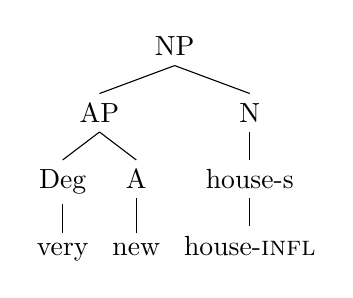
\begin{tikzpicture}
\tikzset{level 1+/.style={level distance=2\baselineskip}}
\tikzset{frontier/.style={distance from root=6\baselineskip}}
\Tree [.{NP} [.{AP} [.{Deg} {very} ] [.{A} {new} ] ] [.{N} [.{house-s} {house-\textsc{infl}} ] ] ]
\end{tikzpicture}
}
\parbox[t]{.45\textwidth}{
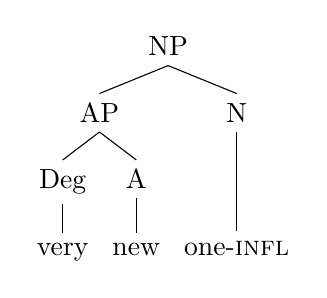
\begin{tikzpicture}
\tikzset{level 1+/.style={level distance=2\baselineskip}}
\tikzset{frontier/.style={distance from root=6\baselineskip}}
\Tree [.{NP} [.{AP} [.{Deg} {very} ] [.{A} {new} ] ] [.{N} {one-\textsc{infl}} ] ]
\end{tikzpicture}
}
\todo{check spacing after trees}

Being a grammatical word, hence a constituent in the phrase structure, the article \textit{one} in English\il{English} is sometimes described as “dummy head” (cf.~e.g.~\citealt[23]{rijkhoff2002}) replacing the noun at the syntactic head position. Consequently, it could be argued that the syntactic head position is never empty in English\il{English}.%??Fn zu Inkorporation unten

\subsection{Appositional modification} \label{apposition}

Apposition\footnote{Note the different meaning of “juxtaposition”, which is defined as a distinct functional type in Section \ref{juxtaposition}.} is commonly described as a sequence of two (or more) co-referential constituents on the same syntactic level and hence with the same syntactic function, as in the following expression.
%%%
\ea
$(_{np} [_{NP}$ Alma and Iva$] [_{NP}$ my daughters$] )$ are in this picture. \label{almaiva}
\z
%%%
Syntactically, the two independent noun phrases \textit{Alma and Iva, my daughters} together serve as one argument phrase in (\ref{almaiva}).\footnote{The annotation of the appositional unit in round brackets is borrowed from \citet[21]{rijkhoff2002}.} In other words, apposition can be defined as a single semantic phrase which consists of several independent syntactic phrases serving one syntactic function together.

\emph{Appositional modification} differs from true apposition because the apposed constituent phrase is semantically and syntactically dependent on the other constituent phrase. Similar to the definition presented in \citet[22]{rijkhoff2002}, appositional (noun) modification is here understood as a construction in which the dependent constituent is not part of the (integral) phrase headed by the modified noun. Semantically, the appositional modifier is headed by the modified noun. Syntactically, however, the appositional modifier has an empty head which is co-referential with the head noun of the apposed noun phrase.

Appositional modification seems to occur as a secondary marked type of adjective attribution marking in several languages, for instance in Georgian\il{Georgian}. Attributive adjectives are normally preposed and show only limited agreement (\ref{georgian unmarked1}). In postposition (marking emphasis), however, the adjective inflects for the full set of cases and numbers (\ref{georgian marked1}). This construction thus resembles an independent (headless) noun phrase in apposition to the semantic head (\citealt[652, 677]{testelec1998}; cf.~also below Section \ref{georgian synchr}).
%%%
\begin{exe}
\ex {\rm Georgian\il{Georgian} \citep[652]{testelec1998}}
\begin{xlist}
\ex \label{georgian unmarked1}
\gll	am or \textbf{lamaz} kal-s\\
	that:\textsc{obl} two nice:\textsc{obl} woman-\textsc{dat}\\
\glt	‘to those two nice women’
\ex \label{georgian marked1}
\gll	kal-eb-s \textbf{lamaz-eb-s}\\
	woman-\textsc{pl}-\textsc{dat} nice-\textsc{pl}-\textsc{dat}\\
\glt	‘to the NICE women’
\end{xlist}
\end{exe}
%%%
Even without differentiated attribution marking, constituent order change between attribute and head can indicate apposition, as in Bulgarian\il{Bulgarian}. Note that the constituent order in noun phrases of Bulgarian\il{Bulgarian} is strictly head-final. In poetic language, however, it is possible to move the adjective after the noun.
%%%
\begin{exe}
\ex {\rm Bulgarian\il{Bulgarian} (own knowledge)}
\begin{xlist}
\ex 	
\gll	tezi \textbf{golem-i} gradove\\
	these big-\textsc{pl} towns\\
\glt	‘these big towns’
\ex	\label{bulgarian marked}
\gll	tezi gradove \textbf{golem-i}\\
	these towns big-\textsc{pl}\\
\glt	‘these big towns’
\end{xlist}
\end{exe}
%%%
It seems impossible to prove whether Bulgarian\il{Bulgarian} presents an example of appositional modification. The emphasized noun phrase in (\ref{bulgarian marked}) could simply be analyzed as integral noun phrase differentiated from other non-emphasized noun phrases by word order. Georgian\il{Georgian}, however, is different from Bulgarian\il{Bulgarian}. The emphasized noun phrase in (\ref{georgian marked}) exhibits different morpho-syntactic marking due to the additional agreement features (Georgian\il{Georgian}) and is very likely to be analyzed as an attributive appositional construction. 

Evidence for appositional modification as a syntactically distinguished noun phrase type is also found in constructions were the apposed headless noun phrase is overtly marked by means of attributive nominalization (cf.~Section \ref{attr nmlz}). Attributive nominalization can be illustrated with the epithet construction in German\il{German}.
%%%
\ea 
{\rm German\il{German}}\\
$[_{NP}$ Friedrich $[_{NP}$ der Gro{ß}e$] ]$ ‘Frederick the Great’
\z

%
\chapter{The syntax-morphology interface} \label{syntax-morphology-interface}

\section{Morpho-syntax}

An inventory of grammatical features relevant to morphology and its interfaces with semantics and syntax has recently been systematized and presented on-line by Kibort (\citeyear{kibort2008a}; grounded in other work, for instance by \citealt{aronoff1994,corbett1987,carstairs-mccarthy1999,corbett2006,corbett-etal2006,bickel-etal2007})\footnote{A volume on the same topic edited by Anna Kibort and Greville Corbett (\emph{Features: perspectives on a key notion in linguistics}) was announced by Oxford University Press but unfortunately has not yet been published before completion of this thesis in July 2010.} !!?? Kibort's typology of morpho-syntactic features will be evaluated in the following sections. It will be shown that true morpho-syntactic features (i.e.~features not interfacing with semantics) relevant to noun phrase structure are missing but have to be added to such an inventory.

Note that the term “morpho-syntax” is sometimes exaggeratedly used for any type of syntactic construction in which morphological processes take place. It is also commonly used as a homonym for “grammar” thus subsuming all kinds of morphological and syntactic structure of a language. For the present study, however the scopes of syntactic and morphological processes are differentiated from each other. Consequently morpho-syntax is here understood as the interface between syntax and morphology, i.e.~syntactic structure assigning morphology on one or more of its constituents.

\paragraph{Morphological features} True morphological features have only inherent values, i.e.~the assignment of these values is not sensitive to syntax. Morphological features include values which are either fixed, i.e.~supplied on the lexical level, or selected from a range of values. The selection of these values is based only on formal criteria. A prototypical example of a purely morphological feature is inflection class.

\paragraph{Morpho-semantic features} Morpho-semantic features also only have inherent values whose assignment is not sensitive to syntax. The values of morpho-semantic features are selected from a range of values. However, unlike purely morphological features, the selection is based on semantic criteria. A prototypical example of the assignment of a morpho-semantic feature is definite marking.

\paragraph{Morpho-syntactic features} Morpho-syntactic features are sensitive to syntax because either agreement or government is involved in the assignment of their values. In the case of agreement, however, a morpho-syntactic feature belongs per definition both to morpho-syntax – due to its contextual assignment to the agreement target – and to pure morphology (or morpho-semantics) – due to its inherent status to the agreement trigger.

The difference between morpho-syntactic and purely morphological (or mor\-pho-semantic) features can be illustrated by definiteness marking in Albanian, Bulgarian and Rumanian. The definite markers in these three Balkan languages are bound morphemes in postposition, cf.~(\ref{definfl alb}) (\ref{definfl rum}) (\ref{definfl bg}). The syntactic behavior of the definite marker in all three languages is also similar: In noun phrases with modifying adjectives the marker attaches enclitically to the first constituent. 
\begin{exe}
\ex \textsc{Albanian} (Albanian<Indoeuropean; \citealt{buchholz-etal1987}) 
\begin{xlist}
\ex \label{definfl alb}
\gll	djal=i\\
	boy(\textsc{m})=\textsc{def:m.sg}\\
\glt	‘the boy’
\ex \label{encl alb a}
\gll	djal=i 				i 			mire\\
	boy(\textsc{m})=\textsc{def:m.sg} 	\textsc{attr:def.m.sg}	good.\textsc{m.sg}\\
\glt	‘the good boy’
\ex \label{encl alb b}
\gll	i 			mir=i 			djalë\\
	\textsc{attr:def.m.sg} 	good=\textsc{def:m.sg} 	boy(\textsc{m})\\
\glt	‘the GOOD boy’ 
\end{xlist}
\ex \textsc{Rumanian} (Romance<Indoeuropean; \citealt{beyer-etal1987})
\begin{xlist}
\ex \label{definfl rum}
\gll	băiat=ul\\
	boy(\textsc{m})=\textsc{def.m.sg}\\
\glt	‘the boy’
\ex \label{encl rum a}
\gll	băiat=ul 				bun\\
	boy(\textsc{m})=\textsc{def.m.sg} 	good.\textsc{m.sg}\\
\glt	‘the good boy’
\ex \label{encl rum b}
\gll	bun=ul 					băiat\\
	good=(\textsc{m})-\textsc{def.m.sg} 	boy(\textsc{m})\\
\glt	‘the GOOD boy’
\end{xlist}
\ex \textsc{Bulgarian} (South-Sla\-vic<Indoeuropean; own knowledge)
\begin{xlist}
\ex \label{definfl bg}
\gll	momče=to\\
	boy(\textsc{n})=\textsc{def.n.sg}\\
\glt	‘the boy’
\ex \label{encl bg}
\gll	dobro=to 		momče\\
	good=\textsc{def.m.sg}	boy(\textsc{n})\\
\glt	‘the good boy’
\end{xlist}	
\end{exe}
The feature \textsc{species},\footnote{Typical values of \textsc{species} are, for instance, \textsc{definite, indefinite} or \textsc{specific}. The use of the term \textsc{species} (from Latin ‘appearance, form’) is borrowed from Swedish and Finnish grammatical terminology, \cite[cf., e.g.,][]{holm-etal1970,itkonen-t1980a}. It will be used throughout this investigation instead of the commonly known “definiteness” because it seems terminologically odd to have a feature \textsc{definiteness} exhibiting a value with the similar label \textsc{definite}.} however, does not belong to morpho-syntax in all of these three languages. Even though the definite marker shows the same syntactic behavior (i.e.~attaching in second-position), the morphological feature \textsc{species} is sensitive to syntactic government only in Albanian. Whereas definiteness is a purely morpho-semantic feature not involved in any syntactic triggering in Bulgarian and Rumanian, in Albanian a second marker of definiteness occurs on the adjective. This marker is required by syntax through the mechanism of agreement. Hence, only definiteness in the Albanian example is morpho-syntactic. In Bulgarian and Rumanian definiteness is purely morphological.

\section{Morpho-syntactic features} \label{crit eval}

As shown in the previous section, \emph{morpho-syntactic marking} can basically be defined as \emph{morphological marking relevant to syntax}. According to \cite{kibort2008a}, the syntactic relevance of a certain morphological marker is determined by the involvement of this marker in either agreement or government. Kibort's view of morpho-syntax, however, is based on definitions of {agreement} and {government} which imply obligatory interfacing of the respective grammatical features with all three components: morphology, syntax and semantics. Hence, a “more accurate term [\dots] would be ‘morpho-semantico-syntactic’ features” \citep{kibort2008a}. 

Both agreement and government require a syntactic constituent as trigger and another constituent as target of morpho-syntactic marking. Kibort's terms \emph{trigger} and \emph{target} are used in the case of agreement marking, whereas \emph{governor} and \emph{governee} are the respective labels in the cases of government. Consequently, Kibort's \emph{government} covers only morpho-syntactic marking assigned by triggers (governors) which are constituents – like a head noun marked for certain gender and number values triggering gender and number \emph{agreement} on the modifier.

Instances of morphological marking triggered not by constituents but by the syntactic structure as such seem to fall outside the range of Kibort's typology of morpho-syntactic features. A prototypical example of morpho-syntactic marking without a trigger inside the noun phrase is attributive state marking in Persian.
\begin{exe}
\ex \textsc{Persian} (SW-Iranian<Indoeuropean; \citealt{mahootian1997})
\label{persian state}
\begin{xlist}
\ex “Construct state” (i.e.~attributive state)
\gll 	xane-ye bozorg\\
	house-\textsc{construct} big\\
\glt 	‘large house’
\ex “Absolute state” (i.e.~predicative state)
\gll	in xane bozorg ast\\
	\textsc{dem} house(\textsc{absolute}) big is\\
\glt	‘the house is large’
\end{xlist}
\end{exe}
In Persian, a nominal head is obligatorily inflected in the construct state if an adjective is present. The trigger of the head-marking attributive suffix \textit{-ye} in Persian is the syntactic structure alone. Since no other value than [+construct] is assigned, semantics cannot be involved. It could be argued that semantics is relevant to the choice of whether to use the adjective as attribute or as predicate and that the attributive inflection on the head noun is inherent (i.e.~morpho-semantically assigned). Semantics (or pragmatics) is of course relevant to the speaker's decision to utter a noun phrase instead of a predication. Semantics is, however, irrelevant to the argumentation about the syntactic structure requiring certain morphological marking: Once the speaker has made her or his decision, it is the syntactic structure alone which is involved in the assignment of the relevant morphological marking. Consequently, attributive construct state in Persian is an example of true morpho-syntactic marking.

Attributive construct state marking morpho-syntactically similar to the Persian construct state marking occurs in many other languages. In Bulgarian, for instance, some nouns require a special inflection after numerals.
\newpage
\begin{exe}
\ex \textsc{Bulgarian} (S-Sla\-vic<Indoeuropean; own knowledge)
\label{bg state}
\gll 	dva 	stol-a\\
	two	chair{\textsc{(m)-construct}}\\
\glt 	‘two chairs’
\end{exe}
Unlike attributive construct state marking in Persian which occurs obligatorily in noun phrases with different types of modifiers (adjectives, nouns, and some other), attributive construct state marking in Bulgarian is restricted with regard to both dependent and head. Thus, it occurs only in noun phrases in which the modifier is a numeral higher than ‘one’ and in which the head noun belongs to the class of non-human masculines. In Bulgarian grammatical tradition this inflectional marking is called the “counting form”.\footnote{Bulgarian \emph{brojna forma}} The marker originates historically from the genitive singular inflection of masculines. The diachrony, however, does not affect the analysis of this marker as belonging to the morpho-syntactic feature \textsc{state} from a synchronic-typological point of view. Even though attributive construct state marking in Bulgarian is much more restricted than in Persian, it clearly belongs to the same type of syntactically assigned inflection on the head noun.

The term \emph{state} here is adapted from \citet[114–116]{melcuk2006} who defines it as an inflectional category of nouns heading a noun phrase. According to Mel'čuk, the function of morphological state marking is licensing the syntactic relationship between the phrase constituents. In the case of head-marking state, as in Persian and Bulgarian (\ref{persian state}+\ref{bg state}), the head noun is inflected and shows the morphological value [+construct] if it is the governing member in the present syntactic relation (i.e.~the noun phrase). 

Even though \emph{state} in Mel'čuk's (and others') terms is usually associated with head-marking constructions of the Persian type (cf.~example \ref{persian state}), a similar morpho-syntactic mechanism applies to dependent marking construct states in other languages. Consider, for example, Kildin Saami in which the dependent noun phrase of a postposition is obligatorily inflected in the genitive case.
\begin{exe}
\ex \textsc{Kildin Saami} (E-Saamic<Uralic; own knowledge)
\label{state ap kildin}
\gll 	tuel'		al'n\\
	chair\textbackslash\textsc{gen}	on\\
\glt 	‘on the chair’
\end{exe}
It could be argued that the genitive inflection of ‘chair’ in example \ref{state ap kildin} is a morphological value of the feature \textsc{case} assigned to the dependent noun phase by the mechanism of \emph{government}. But since genitive is the obligatory and only possible marker in postpositional phrases in Kildin Saami, there is no motivation for assuming that any case value is marked here. There is no semantic connection to a genitive case which marks a possessor noun in Kildin Saami either.\footnote{This is true from a synchronic point of view. Historically, the origin of the genitive marking in adpositional phrases is easily accounted for and goes back to possessor marking in noun phrases with relational head nouns. But again, the diachrony of a certain marker is not relevant to its synchronic-typological categorization.} Since this modification marker is assigned by the syntax of the specific construction alone, and since the only function of this marker is licensing the given syntactic relation (i.e.~an adpositional phrase), a more appropriate gloss could be \textsc{construct}.

Several languages also exhibit dependent marking construct state in noun phrases. The matching value is usually glossed as \textsc{attributive}. In Kildin Saami, for example, members of one (lexically defined) subclass of adjectives are obligatorily inflected for attributive state if they are used as modifiers in a noun phrase.
\eal {\rm \textsc{Kildin Saami} E-Saamic<Uralic (own knowledge)}\label{state np kildin}
\ex	Attributive adjective (cf.~“attributive state”)\\
\gll 	vīl'k-es'		puaz\\
	white-\textsc{attr}	reindeer\\
\glt 	‘white reindeer’
%%%
\ex	Predicative adjective (cf.~“absolute state”)\\
\gll	puaz lī vīll'k-e\\
	reindeer is white-\textsc{pred}\\
\glt	‘the reindeer is white’
\zl
The assignment of attributive inflection on (adjectival) modifiers of nouns as well as the assignment of genitive inflection on (nominal) modifiers of adpositions thus follow a similar syntactic mechanism in Kildin Saami: A certain syntactic relationship (i.e.~an adpositional phrase or a noun phrase, respectively) is licensed by marking the dependent phrase constituent with the feature \textsc{state}.

Finally, the feature \textsc{state} may not only be dependent-marked, as in Kildin Saami, but can even interfere with other features. Whereas attributive state marking is invariable in Kildin Saami, in other languages it shows interference with semantic values assigned through the mechnism of agreement. The agreement inflection of attributive adjectives in Russian, for instance, marks the syntactically governed feature \textsc{state} simultaneously with the morpho-syn\-tacti\-cally governed features \textsc{number/\-gender/\-case}.
\begin{exe}
\ex \textsc{Russian} (E-Sla\-vic<Indoeuropean; own knowledge)
\label{state np russian}
\begin{xlist}
\ex Attributive adjective inflection (cf.~“attributive state”)
\gll 	belyj	olen'\\
	white:\textsc{attr:m.sg}	reindeer\\
\glt 	‘the white reindeer’
\ex	Predicative adjective inflection (cf.“absolute state”)
\gll	olen' bel\\
	reindeer white:\textsc{pred:m.sg}\\
\glt	‘the reindeer is white’
\end{xlist}
\end{exe}

\section{An ontology of morpho-syntactic features}

Besides introducing a few very basic notions connected to noun phrase structure and adjectival modification, the syntax-morphology interface has been discussed in the theoretical sections above. In particular, Kibort's (\citeyear{kibort2008a}) inventory of grammatical features relevant to morphology and its interfaces with semantics and syntax have been critically evaluated. True morpho-syntactic features (i.e.~features not interfacing semantics) are not yet included in her inventory of grammatical features. The argumentation in the present chapter aims at establishing a new feature \textsc{state}, which according to Kibort's own definitions must be regarded as a true morpho-syntactic feature and which should definitely be added to Kibort's (\citeyear{kibort2008a}) list. 

Figure \ref{features figure} shows the morpho-syntactic features relevant to the present inventory of noun phrase types. Note that only the rightmost feature (6) in that figure can be characterized as being of true \emph{morpho-syntactic} nature. The group of features under (5) must be characterized as \emph{morpho-semantico-syntactic} because the syntactic assignment of these features on the agreement target requires their semantically based assignment on the agreement trigger as well. The group of features under (2–4) are \emph{morpho-semantic} features. The group (1) is purely \emph{morphological}. Note also that the feature \textsc{case} shows up in several leaves because  it can be assigned both in morpho-syntax (through agreement on adjectives) or in morphology (through the assignment of either grammatical or semantic cases on head nouns). 
\begin{figure}[htbp]%!!??check
\centerline{
\Tree [.{Morphological\\marking} [.{Inherently\\assigned} [.{Fixed\\(lexically\\supplied)} [.{Based on\\formal\\criteria} [.{e.g.\\\textsc{class}} {1} ] ] [.{Based on\\semantic\\criteria} [.{e.g.\\\textsc{gender}} {2} ] ] ] [.{Selected} [.{Based on\\formal\\criteria} [.{e.g.\\\textsc{number},\\\textsc{case} (gram-\\matical)} {3} ] ] [.{Based on\\semantic\\criteria} [.{e.g.\\\textsc{species},\\\textsc{case} (se-\\mantic)} {4} ] ] ] ] [.{Contextually\\assigned} [.{Determined\\through} [.{Agreement} [.{e.g.\\\textsc{gender},\\\textsc{number},\\\textsc{case},\\\textsc{species}} {5} ] ] ] [.{Determined\\through} [.{(Syntactic)\\Government} [.{e.g.\\\textsc{state}} {6} ] ] ] ] ]\\
}
\caption[Ontology of morpho-syntactic features]{An ontology of morpho-syntactic features relevant to the present inventory of noun phrase types (adapted from Kibort \citeyear{kibort2008a} and extended with the feature \textsc{state})}
\label{features figure}
\end{figure}
In the next part of this investigation, dependent marking \emph{state} will be dealt with in more detail since this type occurs in several languages of the geographic area under investigation.



\part{Typology} \label{part typ}


\chapter{Typologizing noun phrase structure}

The goal of the following chapters is to typologize noun phrases and to present a comprehensive ontology of different syntactic, morpho-syntactic, and morpho-semantico-syntactic attribution marking devices attested in the languages of northern Eurasia and beyond. 

In order to illustrate the different noun phrase types to which these devices belong, data from several languages both within and outside the geographic area of investigation are taken into consideration. The focus, however, will be on constructions and features especially relevant to adjective attribution in the northern Eurasian area.

The term \emph{noun phrase type} used here denotes the specific syntactic or morpho-syntactic structure type of a noun phrase. This term is thus superordinate and belongs to noun phrase structure in general. Since the present study is restricted to a rather small subset of noun phrases, namely noun phrases with adjectival modifiers, the subordinated term \emph{adjective attribution marking device} (instead of \emph{adjective attribution marking type}) will be used to cover all grammatical operations which license the syntactic relation of adjective attribution.

\paragraph{Attribution marking} Minimally, an attribution marking device will simply license the syntactic structure without ranking single constituents, i.e.~without licensing any of the constituents as head or dependent. This is the case for the pure syntactic devices \emph{juxtaposition} and \emph{incorporation}.

The syntactic relation of attribution can also be licensed by a device linking the modifying and the modified constituents morphologically to each other, namely in the case of agreement marking. The morphological device of \emph{agreement marking} is characterized by the assignment of an inherent (i.e.~true morphological) feature from one constituent to another through morpho-syntactic government.

A different instance of “indirect” licensing of attribution is the marking of a semantic relation between the modifier and the modified, as with possessor case (genitive) marking.

It is not at all unusual that the syntactic, morphological, and/\-or semantic relations between noun phrase constituents are marked simultaneously. If, for instance, an attributive construct marker is attached to a modifier which additionally inflects for head-driven agreement, both the syntactic and the morphological relation between the noun phrase constituents are marked. Another example for simultaneously marked syntactic and semantic relations is a noun phrase with a case marked possessor noun (e.g.~in genitive case) and a head noun which is additionally marked for dependent-driven agreement (e.g.~with a cross-referencing possessive affix).

\paragraph{Typological parameters} Noun phrase types with formally distinct characteristics can be defined according to several parameters. Such parameters are, for example, the order of constituents inside the noun phrase (e.g., attribute-head order, head-attribute order, free order), the attribution marker's locus (e.g., on-head, on-dependent), the marker's behavior relative to the whole phrase (e.g.~clitic), its phonological fusion (e.g., free, bound, non-linear), or its position relative to the word host (e.g., pre, post, circum).\footnote{These parameters, adapted from Croft's (\citeyear[93–94]{croft1995}) typological classification of genitive constructions, are applied for a general typology of noun phrase structure in the noun phrase structure module of AUTOTYP (cf.~\citealt{AUTOTYP-NP}).}

Examples for a variety of phonologically, morphologically, syntactically, and semantically distinct types of attribution marking devices will be given in the following chapter. The focus of the ontology presented here is on morphological and morpho-syntactic parameters, especially with regard to the absence or presence of additional attribution marking morphemes, as well as to their kind and behavior. An overall picture of the ontology of attribution devices relevant to this study is given in Figure \ref{tree ontology} at the end of Chapter \ref{ontology}.

Noun phrase types can also be defined on a polyfunctionality scale with regard to the class of modifying elements: Attributive adjectives and other adnominal modifiers (demonstratives, bare nouns, noun phrases, adpositional phrases, clauses, etc.) may or may not occur in similar noun phrase types. The polyfunctionality parameter even takes the content of certain devices beyond attribution marking into consideration. Since the present study investigates adjective attribution marking, the polyfunctionality of attribution marking devices will be dealt with in less detail (see Chapter \ref{polyfunctionality}). 

\paragraph{How many noun phrase types does a language exhibit?} Most languages exhibit more than one distinct noun phrase type because different classes of attributed elements may occur in noun phrase structures which behave differently in their syntax or morpho-syntax. In English, for instance, adjectives and clauses are attributed by means of different devices: Whereas attributive clauses can be attributed by means of relativization (\textit{the dog \textbf{which is nice}}), adjectives are normally juxtaposed (\textit{the \textbf{nice} dog}). Since the present study is devoted to the morpho-syntax of one single class of adnominal modifiers, namely adjectives, variation in attribution marking devices across different classes of attributed elements is of minor importance. 

Nonetheless, attributed elements belonging to one and the same class may also occur in noun phrases which are marked differently: Possessive pronouns in English, for example, can be attributed either by means of juxtaposition (\textit{\textbf{her} dog}) or by using them in a prepositional construction (\textit{the dog \textbf{of hers}}). Even attributive adjectives may occur in two formally distinct noun phrase types. In Turkish, for instance, attributive adjectives are unmarked (\textit{\textbf{kara} kalem} ‘black pencil’); in headless noun phrases marked as direct objects, however, adjectives must be nominalized by means of the 3\textsuperscript{rd} person singular possessive suffix (\textit{\textbf{kara-sını}} ‘the black one (=pencil)’ [\textsc{poss:3sg.acc}]; see also below Section \ref{turkish synchr}). 

Prototypically, the use of different devices for licensing one and the same class of attributed elements is not arbitrary but governed by constraints. Nominalization of adjectives in Turkish, for instance, is due to a syntactic subset constraint affecting those phrases in direct object position and without a lexical head noun. In other languages, the occurrence of a given noun phrase type may also be constrained lexically and/\-or semantically by subsets of either attributes or heads. A well-known example beyond adjective attribution comes from languages in which the choice of possession marking devices is determined semantically by the animate or inanimate subset of the head noun (i.e.~the possessed). Even other subsets of head nouns are known to constrain the choice of possession marking in some languages, such as kinship terms, (non-) referential nouns, etc.

Similarly, languages may exhibit subset constraints on the semantic class of heads modified by adjectives. The epithet-construction marked with an attributive article in English (or other Germanic languages, cf.~\textit{Frederick \textbf{the Great}, Friedrich \textbf{der Große}}; see also below Section \ref{attr nmlz}) may serve as an example. In English, this special noun phrase type only occurs if the head noun belongs to the semantic subclass of proper nouns. 

Examples of a semantic subset of attributes governing a special attribution marking device are commonly found in languages with contrastive focus marking of adjectives. In Rumanian, for instance, adjective attribution marking is usually characterized by a noun phrase type with head-initial constituent order. A different noun phrase type, formally distinguished by the reversed order of constituents, occurs if the adjective bears contrastive focus (see the Rumanian example (\ref{rumanian wo}) on page \pageref{rumanian wo} below).

Finally, many languages exhibit lexically defined subclasses of adjectives (or other adnominal modifiers) which are sensitive with regard to the required attributive marking. In Albanian, for instance, the members of one adjective class are regularly marked by head-driven agreement whereas the members of another adjective class require an additional agreement marker (see the Albanian example (\ref{albanian ex}) on page \pageref{albanian synchr}).

In many languages these lexical subclasses seem marginal and are thus often mentioned merely \emph{en passant} (if at all) in grammatical descriptions. The adjective \textit{pikku} ‘little’ in Finnish is an example for such a marginal subclass: \textit{pikku} is juxtaposed to the modified noun while other adjectives in Finnish show number and case agreement as a rule \citep[75]{karlsson1999}. Similarly in German a few adjectives like the colors \textit{lila} ‘lavender’ and \textit{rosa} ‘pink’ behave morpho-syntactically different and do not agree with the modified noun. Another example for a marginal subclass of adjectives comes from Itelmen, where attributive adjectives are regularly marked with a special attributive suffix (see the Itelmen example (\ref{itelmen ex}) on page \pageref{itelmen synchr}). Only a few loan adjectives from Russian occur in juxtaposition \citep[60–71]{volodin1997}.

These marginal adjective classes are often hard to come across in a rather broad typological survey. It seems to be one disadvantage of the typological method (i.e.~sampling and coding a huge amount of different languages on the basis of qualitatively highly diverse grammatical descriptions) that interesting cases are often missed due to limited knowledge or understanding of the structure of all particular languages. From a diachronic perspective, however, “irregular” linguistic structures are very important because they often reflect innovative tendencies or archaic features, i.e.~features which are due to language change. Marginal noun phrase types should thus be included in typological surveys if they are discovered.


\chapter[Typology of attribution marking]{A typology of adjective attribution marking devices} \label{ontology}

In the present chapter, different types of adjective attribution marking devices attested in natural languages will be described and systematized with a special focus on their typologization according to the morphology of attributive adjectives.

The term \emph{adjective attribution marking} will be used to refer to a grammatical operation relating an adjectival modifier to its noun head. \emph{Attribution marking device} will be used to subsume both overt and covert grammatical operations which license the syntactic relation of attribution. 

\section[Juxtaposition]{Syntactic attribution marking: juxtaposition} \label{juxtaposition}

Juxtaposition can be defined as an unmarked sequence of phrase constituents in which one constituent is syntactically subordinated to the other. It  has to be distinguished from \emph{apposition}. The latter term is usually used to denote an appositive construction of two noun phrases, as in \textit{Alma, meine Tochter} ‘Alma, my daughter’ or \textit{Iva, die jüngere Tochter} ‘Iva, the younger daughter’ where neither constituent is syntactically subordinated. See also the short discussion in Section \ref{apposition}. Juxtaposition is thus characterized by adjacency of noun phrase constituents alone. There is no construction marker present. Consider the following Komi-Zyrian examples where neither agreement markers or any other additional morphemes are present. The attributive adjective in (\ref{komi juxtap}) is represented by its pure stem form. It does not inflect for any of the categories marked on the head noun.\footnote{Beside \textsc{number}, these categories include \textsc{case} and \textsc{possession} in Komi-Zyrian.}
%%%
\begin{exe}
\ex {\rm Komi-Zyrian \citep{lytkin1966a}}
\begin{xlist}
\ex
\gll 	bur 	mort\\
		good	person\\
\glt		‘good person’
\ex
\gll 	bur	mort-jas\\
		good	person-\textsc{pl}\\
\glt		‘good people’
\end{xlist}
\end{exe}
%%%
Juxtaposition constitutes a very widespread attribution mar\-king device cross-linguistically. Among the northern Eurasian languages, juxtaposition occurs as the default attribution marking device in several families, among others in Mongolic, Turkic and Uralic. Whereas juxtaposition constitutes the default type even in the proto-stages in these language groups, the occurrence of juxtaposition in several other languages results from a relatively recent linguistic change in which the original agreement marking on adjectives was lost.

Defining juxtaposition as a “device” for marking attribution might, however, be questionable. Given the definition that attribution is licensed by the sequence of constituents alone, i.e.~that an adnominal modifier and a head noun occur next to each other in the syntactic structure, juxtaposition resembles a “non-marking” rather than a marking device. In English, for instance, one could also argue that the non-occurrence of the copula \textit{is/\-are} is relevant to the marking of attribution. In order to use an adjective as predicate in English (\textit{the man \textbf{is} good, the men \textbf{are} good}), the copula is obligatory. However, word order may be relevant, too. In English, again, juxtaposed attributive adjectives precede the noun as a rule, whereas predicative adjectives follow it. 

Word order can in fact be crucial in languages were both adjective attribution and predication are marked simply through adjacency of noun and adjective but with reversed word order, as for example, in Ainu or Kalmyk. 

\begin{exe}
\ex \textsc{Ainu (Shizunai)} (isolate; \citealt{refsing1986})
\begin{xlist}
\ex
\begin{xlist}
\ex Attribution: adjective-noun order
\gll	pirka cep\\
	be\_good fish\\
\glt	‘a fine fish’
\ex Predication: noun-adjective order
\gll	cep pirka\\
	fish be\_good\\
\glt	‘the fish is fine’\end{xlist}

\ex \textsc{Kalmyk} (Mongolian<Mongolic; \citealt{jachontova1997})
\begin{xlist}
\ex Attribution: adjective-noun order
\gll	čyɣan časun\\
	white snow\\
\glt	‘white snow’
\ex	Predication: noun-adjective order
\gll	časun čyɣan\\
	snow white\\
\glt	‘the snow is white’
\end{xlist}
\end{xlist}
\end{exe}
The only difference between attribution and predication of adjectives in Ainu\footnote{Note that there are no true adjectives in Ainu. Property words are stative verbs in this language (see also section \ref{ainu synchr}).} and Kalmyk is in word order. 
		
\section[Incorporation]{Covert morpho-syntactic construct marking:\\adjective incorporation} \label{attr incorporation}

Similarly to juxtaposition, \emph{adjective incorporation} is characterized by adjacency of phrase constituents. There is no additional morpheme present in this type of noun phrase either. The syntactic relation of attribution is, however, marked by a syntactic composition of modifier and head noun. This type can thus be characterized as covertly marked operation.

\begin{exe} 
\ex \textsc{Västerbotten-Swedish} (N-Germanic<Indoeuropean; \citealt{larsson1929}) \label{bondska compound}
\begin{xlist}
\ex
\gll 	stor-båt-en\\	
	big-boat-\textsc{def:m.sg}\\
\glt	‘the big boat’
\ex
\gll 	stor-hus-et\\
	big-house-\textsc{def:n.sg}\\
\glt	‘the big house’
\end{xlist}
\end{exe}
Since adjective incorporation in northern North-Germanic dialects is syntactically and semantically distinguishable from derivational compounding it is often referred to as \emph{Adjective-Noun-Incorpo\-ration} (for instance by \citealt{sandstrom-etal2003}; \citealt[119–124]{dahl2007} or \citealt[61]{julien2005}).

\paragraph{Phonological vs. syntactic compounds} In Västerbotten-Swedish (as well as in other North-Germanic varieties where adjective-noun compounds occur), accent patterns clearly indicate that adjectives are morpho-phonologically compounded \citep[cf.][]{dahl2003}. Non-compounded monosyllabic stems, such as \textit{tré}, ‘tree’, \textit{bǻt} ‘boat’, \textit{bǻt-er} ‘boats’, \textit{bǻt-er-na} ‘the boats’, have an acute accent (marked with ´ in the examples) as a rule and whether or not they are equipped with inflectional affixes. Bisylabic stems, including compounds, by contrast have pitch accent on the stem (marked with ´ ` in the examples). Compare \textit{tré-bå̀t-en} ‘the wooden boat’ or \textit{stór-bå̀t-en} with the noun phrase \textit{bǻt-en mín} ‘my boat’, where both the noun and the (non-compounded) possessive pronoun have acute accent.

Phonological composition, however, cannot be sufficient evidence for syntactic compounding (i.e.~incorporation). Phrase internal phonological or pro\-sodic processes at the juncture of adjectives and nouns (as, e.g., the accent pattern described above) seem to be very common in languages. Such processes can perhaps prove morpho-phonological composition. For the present typology, however, adjective incorporation is defined purely syntactically as a noun phrase where the attributive adjective occurs obligatorily as a (syntactically) bound morpheme. To prove syntactic boundedness one has to show that the adjective cannot occur unbound. In Västerbotten-Swedish (and other North-Swedish dialects), for instance, the adjective stem cannot occur unbound unless alternative morpho-syntactic marking is applied. Using the adjective ‘big’ in Västerbotten-Swedish in a headless noun phrase results in a construction in which the adjective is marked for agreement and is obligatorily followed by en article serving as a dummy head.\footnote{This is true, however, only with the indefinite adjective. The definite adjective, by contrast, does not need a dummy head but is unbound (and equipped with the definite marker): {\it	stor-en} [big(\textsc{m}) \textsc{def:m.sg}] ‘the big one (masculine)’, \textit{stor-et} [big(\textsc{m}) \textsc{def:n.sg}] ‘the big one (neuter)’.}

\begin{exe} 
\ex \textsc{Västerbotten-Swedish} \label{bondska headless}
\begin{xlist}
\ex
\gll 	en stor en\\	
	\textsc{indef:m} big(\textsc{m}) \textsc{art:indef:m.sg}\\
\ex
\gll 	ett stor-t ett\\	
	\textsc{indef:n} big:\textsc{n} \textsc{art:indef:n.sg}\\
\glt	‘a big one’
\end{xlist}
\end{exe}
If evidence for syntactic incorporation cannot be found compounded adjectives can only by described as a special case of juxtaposition. But interestingly, if the described test of syntactic boundedness is applied, then English falls in the category of incorporating languages as a result. In English too, attributive adjectives can only occur bound to a head. This head is either lexical or, similar to Västerbotten-Swedish indefinite noun phrases, an obligatory article as dummy head.\footnote{Applying the same test, it turnes out that English incorporates even other modifiers of nouns, such as possessive pronouns: \textit{give me her book} – \textit{give me her-s}.}

Whether or not English is coded as an incorporating language, adjective incorporation seems to constitute a minor type of attribution marking. Among languages of the northern Eurasian area, however, this type is attested in geographically quite distinct languages: besides the peripheral North-Germanic dialects, it is also found in Adyge and in Chukchi, Kamchatkan and in Eskimo-Aleut languages (see the respective sections of Part \ref{part synchr}).

\section[Agreement]{Morpho-semantico-syntactic attribution\\marking: agreement}

\emph{Agreement} (aka \emph{concord}) is a common type of overt attribution marking device. Agreement is commonly understood as a systematic covariance between a semantic or formal property of one element and a formal property of another \cite[610]{steele1978}. In other words, agreement can be defined as the spread of semantic or morphological properties across constituents of a syntactic phrase. The agreement properties (or \emph{agreement features}) spread from “trigger constituents”\footnote{In other terms, the trigger of agreement can be called \emph{controller}, cf.~\citealt{corbett2006}.} and are formally, i.e.~morphologically expressed on “target constituents”.

The primary syntactic function of agreement is to relate phrase constituents to each other. Agreement thus serves the formal licensing of dependency in the given phrase. As compared to construct marking, however, the licensing of dependency by means of agreement is more the indirect result of morphological copying of agreement features across phrase constituents.

In principle, agreement features can be triggered by both syntactic heads and syntactic dependents, as will be shown in the following sections. Based on where the agreement features originate, the terms \emph{head-driven} and \emph{dependent-driven agreement}, first proposed by Balthasar Bickel and Johanna Nichols in 2001 \citep[published as][]{bickel-etal2007}, will be used in the following.

\subsection{Head-driven agreement} \label{head-driven agreement}

Typical morpho-syntactic agreement features triggered by syntactic heads are \textsc{gender, number} and \textsc{case}, as in Lower Sorbian.

\begin{exe}
\ex \textsc{Lower Sorbian} (W-Sla\-vic<Indoeuropean; \citealt{janas1976}) \label{sorbian agr}
\begin{xlist}
\ex
\gll	dobr-y cłowjek\\
	good-\textsc{sg:m} person(\textsc{m})\\
\glt	‘a good person’
\ex
\gll	dobr-e cłowjek-y\\
	good-\textsc{pl} person-\textsc{pl}\\
\glt	‘good people’
\ex \label{ap case gov}
\gll	k dobr-emu cłowjek-oju\\
	to good-\textsc{sg:m:dat} person-\textsc{sg:m:dat}\\
\glt	‘to a good person’
\end{xlist}
\end{exe} 
Note, however, that Kibort (\citeyear{kibort2008a}; following \citealt[133–135]{corbett2006}) does not list \textsc{case} as a prototypical agreement feature. In Kibort's and Corbett's view, the matching of a case value on the noun phrase head and its adjectival (or other) modifier(s) does not count as “canonical agreement” but is simultaneously imposed on the noun phrase constituents as the result of government by a syntactic element outside the noun phrase. Consider the Lower Sorbian example (\ref{ap case gov}) in which both the adjective ‘good’ and the noun ‘person’ are marked with the dative case suffix.

The question is whether the case value in such examples is imposed on both noun phrase constituents through government (in example \ref{ap case gov} by the preposition \textit{k} ‘to’) as argued by Kibort and Corbett, or if the dative case on the modifying adjective is imposed by its head by means of agreement, similar to gender and number agreement which are also imposed by the head noun. Adopting Mel'čuk's (\citeyear[329, 337]{melcuk1993}) dependency view of syntax instead of Corbett's (\citeyear[133]{corbett2006}) “constituency”, the dependent constituent in the adposition phrase is a noun phrase. The dependent constituent in the noun phrase, again, is an adjective phrase (i.e.~the attributive adjective) which depends on the noun head of the phrase and inherits its case marking. In this view, the morpho-syntactic mechanisms of assigning a head's morphological features to dependent constituents are similar for case and other agreement categories (like gender and number). Consider (\ref{ap case gov}) ‘to a good person’ in Lower Sorbian.

\begin{exe}
\ex \textsc{Lower Sorbian}\\%[ $_{AdP}$ k [ $_{NP}$ dobremu$_{agr}$ cłowjekoju$_{gender:number:case}$ ] ]
\end{exe}
Another possible agreement feature beside \textsc{gender, number} and \textsc{case} is \textsc{species}, typical values of which are \textsc{definite} and \textsc{indefinite}. Consider, for instance, the agreement paradigm of adjectives in Icelandic (Table \ref{icelandic agr}) in which indefinite and definite forms are distinguished.

Cross-linguistically, head-driven agreement seems to be a wide-spread attribution marking device across the world's language families. The actual morphological appearance of agreement marking, however, is highly diverse across languages and depends on several parameters.

One such parameter concerns the form of the agreement marking morphemes in comparison to the morphemes marking the respective values on the head noun. In fact, adjective agreement paradigms in many languages are different from the respective inflectional paradigms of nouns. This is true, for instance, for Sla\-vic and Germanic languages, as mentioned, but also for other Indoeuropean languages. 

\begin{table}
\begin{footnotesize}
\begin{center}
\begin{tabular}[t]{l l | l l l | l l l}
		\hline
		\hline
		&		&\textsc{m.sg}&\textsc{f.sg}&\textsc{n.sg}&\textsc{m.pl}&\textsc{f.pl}&\textsc{n.pl}\\
		\hline
		&\textsc{nom}	&–ur		&–Ø	&–t		&–ir		&–ar		&–Ø \\
\textsc{indef}	&\textsc{acc}	&–an		&–a	&–t		&–a		&–ar		&–Ø \\
		&\textsc{dat}	&–um		&–ri	&–u		& –um&–um&–um\\
		&\textsc{gen}	&–s		&–rar	&–s		& –ra&–ra&–ra\\
		\hline
		&\textsc{nom}	&–i		&–a		&–a		&\multicolumn{3}{c}{–u}\\
\textsc{def}	&\textsc{acc}	&–a		&–u		&–a		&\multicolumn{3}{c}{–u}\\
		&\textsc{dat}	&–a		&–u		&–a		&\multicolumn{3}{c}{–u}\\
		&\textsc{gen}	&–a		&–u		&–a		&\multicolumn{3}{c}{–u}\\
		\hline
		\hline
\end{tabular}
\end{center}
\end{footnotesize}
\caption[Adjective paradigm for \textsc{Icelandic}]{Adjective declension paradigm for \textsc{Icelandic} (N-Germanic<Indo\-eu\-ro\-pean; \citealt{kress1982})} \label{icelandic agr}
\end{table}
In other languages, however, inflectional suffixes might simply reoccur on the modifier, as in Finnish.
\begin{exe}
\ex \textsc{Finnish} (Finnic<Uralic; own knowledge) \label{finnish agr.}
\begin{xlist}
\ex
\gll 	iso-t		talo-t\\
	large-\textsc{pl}	house-\textsc{pl}\\
\glt	‘large houses’
\ex
\gll 	iso-i-ssa		talo-i-ssa\\
	large-\textsc{pl}-\textsc{iness} house-\textsc{pl}-\textsc{iness}\\
\glt	‘in large houses’
\end{xlist}
\end{exe}
Adjectives and nouns in Finnish (and in most other Uralic languages) differ in syntactic function rather than in morphological properties. Consequently, adjectives and nouns in Finnish exhibit similar inflectional paradigms. Probably, such a weak distinction between adjectival and nominal inflections was also true for proto-Indoeuropean (cf.~\citealt[80]{comrie1998}, \citealt[139]{kuriaki2007}). But the declensions of both adjectives and nouns in Indoeuropean languages have undergone radical changes and have become clearly distinct from each other. This is evident, e.g., in the Lower Sorbian example (\ref{sorbian agr}) on page \pageref{sorbian agr} where the adjective suffix \textit{-emu} and the noun suffix \textit{-oju} both mark the dative masculine singular.

Head-driven agreement marking also deviates across languages in respect to the inventory of morphological categories involved. Many languages exhibit head-driven agreement paradigms which exclude certain inherent or assigned morphological categories of the head noun, as in Finnish, where nouns inflect for \textsc{number}, \textsc{case} and \textsc{possession}. The latter feature, however, never spreads through the noun phrase.
\begin{exe}
\ex \textsc{Finnish} (Finnic<Uralic; own knowledge)
\begin{xlist}
\ex
\gll 	iso		talo-ni\\
	large	house-\textsc{poss:1sg}\\
\glt	‘my large house’
\ex
\gll 	*iso-ni	talo-ni\\
	large-\textsc{poss:1sg}	house-\textsc{poss:1sg}\\
\end{xlist}
\end{exe}
Finally, agreement paradigms can be “defect” in the sense that certain agreement categories do not show up on all members of the paradigm. In Danish, for example, gender as an agreement feature is marked on the attributive adjective only in indefinite noun phrases. In noun phrases marked for definite species, the attributive adjective is marked with an invariable definite agreement suffix. Consider examples (\ref{danish agr ex}) and Table \ref{danish agr paradigm} with the respective paradigm in Section \ref{n-germanic synchr}.

\begin{exe}
\ex \textsc{Danish} (N-Germanic<Indoeuropean; own knowledge) \label{danish agr ex}
\begin{xlist}
\ex
\gll en \textbf{stor} mand\\
	\textsc{indef.com} big.\textsc{utr} man(\textsc{utr})\\
\glt	‘a tall man’
\ex
\gll ett \textbf{stor-t} hus\\
	\textsc{indef.n} big-\textsc{n} house(\textsc{n})\\
\glt	‘a large house’
\ex	
\gll den \textbf{stor-e} mand\\
	\textsc{def.com} big-\textsc{def} man(\textsc{utr})\\
\glt	‘the tall man’
\ex
\gll det \textbf{stor-e} hus\\
	\textsc{def.n} big-\textsc{def} house(\textsc{n})\\
\glt	‘the large house’\end{xlist}
\end{exe}
An extreme case of a defective agreement paradigm is found in Chechen where adjectives only partially agree with the head noun and show only one single case distinction between nominative versus all other cases.\footnote{A similar defective agreement paradigm with only one case distinction is found in Ingush, cf.~Section \ref{ingush synchr}.}
\begin{exe}
\ex \textsc{Chechen} (Chechen-Ingush<Nakh-Daghestanian; \citealt[29]{nichols1994a})\\
\textsc{nom:sg} dika\textsuperscript{n} stag\textsuperscript{3} ‘good person’\\
\textsc{gen:sg} dikaču stega\textsuperscript{n}\\
\textsc{dat:sg} dikaču stagana\\
\textsc{erg:sg} dikaču staga\\
\textsc{all:sg} dikaču stagie\\
\textsc{nom:pl} dika\textsuperscript{n} na:x\\
%\textsc{gen:pl} dikaču ne:xa\textsuperscript{n}\\
\end{exe}

\subsection{Dependent-driven agreement}

In many languages spoken inside and outside the northern Eurasian area, head-driven agreement is attested as a device for licensing attributive modification. The reverse agreement type, \emph{dependent-driven agreement}, is also wide-spread among the world's languages. Among the languages of my sample, however, dependent-driven agreement marking is attested only as a device for the licensing of (possessor) noun attributes. An example of a language with dependent-driven agreement marking in possessive noun phrases is Oroch.
\begin{exe}
\ex 	\textsc{Oroch} (Amur Tungusic<Tungusic; \citealt[3]{malchukov2000}) \label{oroch dep-driven agr.}
\gll 	nia	d'uu-ni\\
	man	house-\textsc{poss:3sg}\\
\glt	‘a man's house’
\end{exe}
The possessed noun ‘house’ in example (\ref{oroch dep-driven agr.}) obligatorily agrees with the \textsc{3sg} possessor ‘man’. This type of dependent-driven agreement is usually called \emph{possessor agreement}.\footnote{Another commonly used term is \emph{cross reference marking}.}

\subsubsection{Modifier-headed possessor agreement} \label{ModheadAgr}

The term \emph{modifier-headed possessor agreement} is derived from \emph{modifier-headed agreement} introduced in \citet{AUTOTYP-NP}. It is a subtype of dependent-driven agreement characterized by reverse semantic and syntactic dependency relations between attribute and head. 

Structurally similar to example (\ref{oroch dep-driven agr.}), Oroch also exhibits dependent-driven agreement marking by means of possessive affixes on attributive adjectives.

\begin{exe}
\ex 	\textsc{Oroch} (Amur Tungusic<Tungusic; \citealt[3]{malchukov2000}) \label{oroch mod-headed agr}
\begin{xlist}
\ex
\gll 	nia	aja-ni\\
	man	good-\textsc{poss:3sg}\\
\glt	‘a GOOD man’
\ex 
\gll nia-sa aja-ti\\	
	man-\textsc{pl} good-\textsc{poss:3pl}\\
\glt	‘GOOD men’
\end{xlist}
\end{exe}
In the Oroch example, the semantic head of the noun phrase ‘man’ is syntactically “degraded” to the (dependent) possessor function, and the semantic dependent is “upgraded” to the function of the syntactic head of the phrase, i.e.~the possessed. According to \citet[3]{malchukov2000}, the expression still has an attributive reading: ‘a man, a property of whom is “to be good”’, rather than a possessive one: *“a man's goodness”. Thus, the semantic attribute is rendered as the head (i.e.~the possessed) and the semantic head of the possessive noun phrase takes the slot of the dependent (i.e.~the possessor).

Whereas modifier-headed possessive agreement constitutes a marked structure in Oroch, it can be the universal type of attributive marking on adjectives in other languages. This kind of adjective attribution marking device is not very common in the northern Eurasian area under investigation, but it is pervasive, for instance, in Oceanic languages (cf.~\citealt{ross1998}). In Saliba, for example, attributive adjectives as a rule are marked by means of 3\textsuperscript{rd} person possessive suffixes.

\begin{exe}
\ex \textsc{Saliba} (Western Oceanic<Austronesian; \citealt{mosel1994}) \label{saliba poss-agr}
\begin{xlist}
\ex
\gll 	sine natu-na\\
 	woman child-\textsc{poss:3sg}\\
\glt ‘a woman's child’/\-‘the child of the woman’
\ex
\gll 	sine-o natu-di\\
	woman-\textsc{pl} child-\textsc{poss:3pl}\\
\glt	‘women's children / the children of the women’%(check this example: child or children)
\end{xlist}
\end{exe}
In Saliba, possessor nouns are licensed as modifiers in a noun phrase by means of (dependent-driven) possessor agreement on the head noun. Similar to the marked noun phrase in Oroch (\ref{oroch mod-headed agr}), attributive adjectives are marked by means of modifier-headed possessor agreement.

\begin{exe}
\ex \textsc{Saliba} (Western Oceanic<Austronesian; \citealt{mosel1994} \label{saliba mod-headed agr})
\begin{xlist}
\ex
\gll 	mwaedo gagili-na\\
 eel small-\textsc{poss:3sg}\\
\glt ‘a small eel’
\ex
\gll 	mwaedo gagili-di\\
	eel small-\textsc{poss:3pl}\\
\glt ‘small eels’
\end{xlist}
\end{exe}
The adjectival attribute ‘small’ in example (\ref{saliba mod-headed agr}) occurs in a possessive-like construction (similar to \ref{saliba poss-agr}) where the adjective takes the slot of the possessed and is subsequently marked with a possessive agreement suffix.\footnote{An alternative account of noun phrase structure in Saliba could claim that the verbal attribute is marked by head-driven agreement, analyzing the suffixes \textit{-na} and \textit{-di} as singular and plural markers, respectively. This analysis is obviously underlying the descriptions of Saliba (e.g.~\citealt{mosel1994}, \citealt{margetts1999}), which leave the homophony of \textit{-na} \textsc{poss:3sg} and \textit{-di} \textsc{poss:3pl} with \textit{-na} \textsc{sg} and \textit{-di} \textsc{pl} undiscussed .} % [ON BASIS OF WHAT] I would rather make the claim, that attributive adjectives in Saliba occur in headstand noun phrases and are marked by means of modifier-headed possessor agreement.
Unlike in Oroch, however, modifier-headed possessor agreement is the default type of attributive connection of adjectives in Saliba.

\section[Construct marking]{Overt morpho-syntactic construct marking:\\attributive state marking}

Due to a lack of better terminology the feature \textsc{state} was earlier defined as assigned through \emph{syntactic government} (in Section \ref{crit eval}). Unlike the common notion of \emph{government}, which requires a trigger inside the phrase, true syntactic government considered in this study has no other trigger than the syntactic construction as such.

In order to avoid the misleading term \emph{government}, all overtly marked attribution devices with the exclusive function of licensing the syntactic relation between constituents of a noun phrase are defined here as \emph{attributive state marking}. “Overtly marked” means that (at least one) additional attribution marking morpheme is present in the noun phrase.

\emph{Attributive state} is adopted from “Construct state” or “Status constructus” which are commonly used in syntactic descriptions of languages exhibiting head-marking {state} (e.g.~Persian). Since construct state marking morphemes may occur on different loci inside the noun phrase, \emph{attributive state} will be used as superordinate term, subsuming the subtypes with the following loci of their respective attributive markers:\footnote{Other logically possible loci of attributive state markers would result from simultaneous marking on head- and/\-or on dependent+floating. I am, however, not aware of any language exhibiting such noun phrase types.}

\begin{itemize}
\item{on-head (construct)}
\item{on-dependent (anti-construct)}
\item{neither on-head nor on-dependent (floating construct)}
\item{simultaneously on-head and on-dependent (double construct)}
\end{itemize}
Among the northern Eurasian languages considered in the present study, only the first two types of attributive state marking, i.e.~head-marking state and dependent marking state, are attested as devices for licensing attributive adjectives. These two types are dealt with in more detail below in Sections \ref{head-marking state} and \ref{dep-marking state}.

\subsection{Head-marking attributive state } \label{head-marking state}

The attributive construction in Persian, commonly known as \emph{Ezafe} (or \emph{Izafe}), illustrates a typical case of head-marked attributive state.
\newpage
\begin{exe}
\ex \textsc{Persian} (SW-Iranian<Indoeuropean; \citealt{mahootian1997}) \label{persian constr state}
\gll xane-ye bozorg\\
	house-\textsc{attr} big\\
\glt 	‘a large house’
\end{exe}
The only function of the attributive suffix \textit{-(y)e}\footnote{The allomorph \textit{-e} appears ofter consonants.} on the noun ‘house’ is to show that “I am a noun phrase and I have a dependent.”\footnote{The attributive construct state marking in Persian is polyfunctional in the sense that its function is not restricted to the licensing of adjectives as modifier in a noun phrase, but also of noun attributes, adpositional phrases and infinitives.} The traditional term for the morphological value given by the head-marking attribution device in Persian is \emph{construct state} (or \emph{status constructus}). What is meant hereby is that the noun displays different “states” depending on the presence of a modifier in the noun phrase.

Obligatory attribution marking by means of an Ezafe-construction is also characteristic for other Iranian languages. In Kurmanji, a variety of Kurdish spoken in the northern Eurasian area, the Ezafe-formative is not an invariable suffix – unlike the cognate suffix \textit{-(y)e} in Persian – but also indicates morphological values of \textsc{number} (\textsc{sg/\-pl}), \textsc{gender} (\textsc{m/\-f}) and \textsc{species} (\textsc{def/\-indef}). Consider example (\ref{ez kirmanji ex}) and the paradigm in Table \ref{ez kirmanji paradigm}. 

\begin{exe}
\ex \textsc{Kirmanji} (W-Iranian<Indoeuropean; \citealt{ortmann2002b}) \label{ez kirmanji ex}%CHECK source
\begin{xlist}
\ex
\gll	kur-\^e mezin\\
	boy-\textsc{attr:def.m.sg} big\\
\glt	‘the tall boy’
\ex	
\gll	ke\c{c}-a ba\c{c}\\
	girl-\textsc{attr:def.f.sg} nice\\
\glt	‘the nice girl’
\ex	
\gll	kur-\^en / ke\c{c}-\^en ba\c{c}\\
	boy-\textsc{attr:def.pl} {} girl-\textsc{attr:def.pl} nice\\
\glt	‘the nice boys/\-girls’ %\cite{ortmann}%glossen
\end{xlist}
\end{exe}

\begin{table}[ht]
\begin{center}
\begin{footnotesize}
\begin{tabular}[t]{l | ccc}
\hline
\hline
		&\textsc{m.sg}	&\textsc{f.sg}		&\textsc{pl}\\
\hline
\textsc{def}	&-(y)\^{e}	&-(y)a			&-(y)\^{e}n\\
\textsc{indef}	&-î		&-e				&\\
\hline
\hline
\end{tabular}
\caption[Paradigm of the Ezafe in \textsc{Kurmanji}]{Paradigm of the Ezafe in \textsc{Kurmanji} \citep{schroder2002}} \label{ez kirmanji paradigm}
\end{footnotesize}
\end{center}
\end{table}
\noindent Note that the values of true morphological features (\textsc{number, gender, species}) of the noun are combined with the morpho-syntactic feature \textsc{attributive} in the differentiated forms of the Ezafe in Kirmanji. But agreement is not involved here because gender, number and species marking is not triggered within the noun phrase but is inherited to the head noun morpho-semantically.

\subsection{Dependent marking attributive state}\label{dep-marking state}

\subsubsection{Anti-construct state} 
In some languages there is an attributive construction corresponding to the Iranian Ezafe, which however does not mark the head but the adjectival dependent for “state” (i.e., indicating the availability of a head in the present noun phrase). This type of marking occurs, for instance in Saamic languages.

\begin{exe}
\ex \textsc{Kildin Saami} (E-Saamic<Uralic; own knowledge)
\begin{xlist}
\ex Predicative state \label{kildin pred.adj.}
\gll Tedt 	pērrht l{ī} ēll.\\
	\textsc{dem} house \textsc{cop} high\\
\glt	‘This house is high.’
\ex Attributive state
\begin{xlist}
\ex	\label{kildin attr.adj.sg}
\gll Tedt	l{ī} 	ēl'l'\textbf{-es'} 		pērrht.\\
	\textsc{dem} \textsc{cop}	high-\textsc{attr}	house\\
\glt	‘This is a high house.’
\ex	\label{kildin attr.adj.pl}
\gll Tegk 	liev 	ēl'l'\textbf{-es'}		pērht.\\	
	\textsc{dem}	\textsc{cop}	high-\textsc{attr} house$\backslash$\textsc{pl}\\
\glt	‘These are high houses.’
\end{xlist}
\end{xlist}
\end{exe}
Whereas the predicatively used adjective ‘high’ is represented by its pure stem form (\ref{kildin pred.adj.}), it is marked with the attributive suffix \textit{-es'} if used as modifier (\ref{kildin attr.adj.sg}+\ref{kildin attr.adj.pl}). Attributive marking on adjectives in Kildin and other Saamic languages is highly irregular due to the strong tendency to merge predicative and attributive adjective forms. Other adjective marking devices also occur. The default type in most Saamic languages, however, is that attributive adjectives exhibit an attributive inflection (\citealt{riesler2006b}; see also below section \ref{saami synchr}).

The attribution marker in Saamic is invariable, i.e.~the adjective does not show agreement with its head noun. The host of the Saamic attributive suffix is the adjective. Its only function is to specify the syntactic relation between head noun and adjectival modifier (“my host is dependent in the present syntactic structure”). Since the construction in Saamic constitutes dependent marking opposite to the Persian construct state, it can be labeled \emph{anti-construct}.\footnote{The term was introduced during Bickel's and Nichols' earlier work on the AUTOTYP Noun Phrase Structure Database, cf.~\citet[2, elsewhere]{bickel-etal2002}, \citet{AUTOTYP-NP}.} 

Anti-construct state marking seems not uncommon cross-linguistically, even if Saamic and the Iranian language Northern Talysh (cf.~Section \ref{talysh synchr}) provide the only examples of European languages with anti-construct state marking on adjectives. Note that typological descriptions and grammars use quite different terms for anti-construct state markers, such as \emph{attributive particle}, \emph{relator}, \emph{associative marker}, \emph{linker}, etc. If anti-construct marks the attribution of possessor nouns (besides adjectives) it is also often called \emph{attributive case} or \emph{genitive}.

\paragraph{Possessive case marking} 
From a purely syntactic point of view, possessive case marking is similar to anti-construct state marking. Both are syntactically governed dependent marking devices. In fact, anti-construct state marking of adjectives is sometimes described as “genitive” if the device is polyfunctional and marks possessor nouns as well.\footnote{Even other construct marking devices, such as the linker in Tagalog (\ref{tagalog linker}) or the construct state marker in Persian (\ref{persian constr state}) are often described as “genitives” because they mark possession. Unlike prototypical genitives, however, the construct markers in Tagalog and Persian do not constitute dependent marking devices.} Rather than extending the terminological domain of possessive case marking to adnominal modifiers beyond noun possessors, the term \emph{possessive case} (or \emph{possessor case}) will be used here only for describing a special subtype of anti-construct state. Whereas the latter is a purely morpho-syntactic device, possessive case additionally specifies a semantic relation (i.e.~possession).

\subsubsection{Anti-construct state agreement marking} \label{anti-constr agr}
Construct state markers such as the linker in Tagalog, the head-marking construct state marker \textit{-(y)e} in Persian, or the dependent marking anti-construct state marker \textit{-es'} in Kildin Saami are proper construct state markers in the sense that they are exclusively used as licensee of an attributive syntactic relation between modifying and modified constituents in the noun phrase. The respective formatives thus have morphologically unalterable shapes.

In other languages, however, certain adnominal modifiers marked for anti-construct state may additionally be the target of either head- or dependent-driven agreement. Such combined agreement and construct marking devices should consequently be characterized as simultaneously marking the syntactic and the morphological relation between the noun modifier and the modified noun. 

This subtype of anti-construct state marking, characterized by (adjectival or other) adnominal modifiers being marked simultaneously for anti-construct state and for head-driven agreement, will be labelled \emph{anti-construct state agreement marking} in the following.\footnote{The extended label \emph{\textbf{head-driven} anti-construct state agreement marking} seems obsolete because the agreement is self-evidently triggered by the head noun in this type.} %Aber warum zähle ich es zu Konstruktionsmarkierung und nicht als Untertyp von Kongruenz?

A typical example of a language with anti-construct state agreement marking is Russian.

\begin{exe}
\ex \textsc{Russian} (E-Sla\-vic<Indoeuropean; own knowledge) \label{ru-anti}
\begin{xlist}
\ex	Anti-construct state agreement
\begin{xlist}
\ex
\gll 	vysok\textbf{-ij} 			dom\\
	high-\textsc{attr:m.nom} house(\textsc{m})\\
\glt	 ‘(a/\-the) high house’
\ex
\gll 	vysok\textbf{-aja} 			bašn'a\\
	high-\textsc{attr:f.nom} tower(\textsc{f})\\
\glt	 ‘(a/\-the) high tower’
\end{xlist}
\ex
\begin{xlist}
\ex Predicative agreement
\gll 	Etot 	dom	vysok\\
	\textsc{dem:m} house(\textsc{m}) 	high:\textsc{m}\\
\glt	 ‘this house is high’
\ex
\gll 	Eta 	bašn'a	vysoka\\
	\textsc{dem:f} tower(\textsc{f}) 	high:\textsc{f}\\
\glt	 ‘this house is high’
\end{xlist}
\end{xlist}
\end{exe}
In Russian, attributive as well as predicative adjectives show agreement in \textsc{gender} and \textsc{number}. Attributive adjectives agree additionally in \textsc{case}. The agreement suffixes of the attributive and predicative paradigms, however, have different shapes; consider Table \ref{Russian adj agr paradigm}.

Traditionally, the two inflection paradigms of the adjective in Russian have been contrasted to each other as “short” and “long” forms. These terms, however, describe the form rather than the function of the different agreement inflections and are thus less useful for the classification of the Russian noun phrase type from a morpho-syntactic typological perspective. The “long” adjectives of Russian do not simply belong to a different declension paradigm as compared to their “short” counterparts. The formal distinction between the two adjective declensions is connected to attribution marking. Whereas the predicative (“short”) forms show “pure” agreement, the agreement suffixes on attributive adjectives mark agreement and the attributive state of the adjective simultaneously.

Historically, the attributive adjective inflection consists of two morphemes: a pronominal stem plus the original “short” agreement suffix.\footnote{In the forms for nominative (cf.~Table \ref{Russian adj agr paradigm}) the two morphemes for \textsc{attr} and \textsc{gender/number/case} are still separable. In the remaining cases, however, they are merged into one portmanteau suffix.} Synchronically, the attributive adjective suffixes in Russian are thus best analyzed as portmanteau suffixes marking anti-construct and head-driven agreement simultaneously.

One could argue against the analysis of the “long” adjective declension in Russian as attributive state marking saying that “long form adjectives” also occur in predicative position. In fact, the semantic difference between the use of “short” versus “long” forms in adjective predication in Russian could be described as an opposition between temporal and permanent properties denoted by the adjective.
Nonetheless, the marking of the predicative adjective is rather irrelevant here. What is crucial, however, is the use of the “long” forms, which occur in attributive position as a rule. The “short” (i.e.~predicative) form cannot occur in attributive position.

Furthermore, it could even be argued that “long” form adjectives in predicative position are instances of adjective attribution marking rather than of adjective predication. This is the case if one analyses the “long form adjectives” as headless noun phrases in an appositive construction, as the “long” predicative form in (\ref{ru-pred-long}) denoting a permanent property apposed to the “short” predicative form in (\ref{ru-pred-short}) denoting a temporal property.\footnote{Russian examples of morphologically differentiated predicative adjectives also often reflect an opposition in the subject's denotative status. The “short” form is used for denoting reference to a class of objects: \textit{krasavicy \textbf{kaprizn-y}} [capricious-\textsc{pred:agr}] ‘beautiful women are capricious’), the “long” form is used for denoting reference to an individual: \textit{oni \textbf{kaprizn-ye}} [capricious-\textsc{attr:agr}] ‘they are capricious’ (or ‘they are (the) capricious ones’, e.g.~two sisters known from the discourse) (cf.~\citealt[210 Footnote 76]{mendoza2004}).}
\begin{exe}
\ex “Short” and “long” predicative adjectives in \textsc{Russian}
\begin{xlist}
\ex \label{ru-pred-short}
\gll on bolen\\
	3\textsc{sg} ill:\textsc{pred:m}\\
\glt	 ‘he is ill’
\ex \label{ru-pred-long}
\gll on bol'nyj\\
	3\textsc{sg} ill:\textsc{attr:m}\\
\glt	 ‘he is a sick one (i.e.~he is mentally sick)’
\end{xlist}
\end{exe}
The origin of anti-construct state agreement marking in Russian is dealt with in Chapter \ref{slavic diachr}. It is worth mentioning that remnants of an Old Sla\-vic anti-construct adjective inflection are found in other modern Sla\-vic languages as well, especially in the South-Sla\-vic languages Slovenian and Serbian where the “long” adjective forms occur in definite noun phrases (cf.~Section \ref{slovenian synchr}).

Similar to South-Sla\-vic but much more regular is the occurrence of a cognate anti-construct adjective inflection in the Baltic languages Latvian and Lithuanian.

\begin{exe}
\ex \textsc{Latvian} (Baltic<Indoeuropean; \citealt[115]{dahl2007})
\begin{xlist}
\ex	\label{latvian indef}
\gll liel-a māja\\
	big-\textsc{f.nom.sg} house(\textsc{f})\\
\glt	‘a large house’
\ex	\label{latvian def}
\gll liel-ā māja\\
	big-\textsc{attr:f.nom.sg} house(\textsc{f})\\
\glt	‘the large house’
\end{xlist}
\end{exe}
Unlike in Russian where attributive adjectives are marked with the anti-con\-struct state agreement suffixes as a rule, the use of the cognate attributive forms in the Baltic languages is usually described as depending on the referential status of the head noun. Whereas the “short form” agreement suffix is used with adjectives modifying indefinite nouns (\ref{latvian indef}), the attributive adjective in definite noun phrases is obligatorily marked with the “long form” agreement suffix (\ref{latvian def}).

The anti-construct state agreement marking suffixes in the Baltic languages is often described as a definiteness marker. Note, however, that the definite noun never exhibits definite marking itself. If no attributive adjective is present the definite noun remains unmarked. The analysis of the “long form” agreement suffix in Baltic as definite marker would thus presuppose the assumption that the definite marker is selective and shows up only on attributive adjectives. 

Markers which are selective according to their host's parts-of-speech membership are indeed attested.\footnote{Consider, e.g., the two allomorphs of the definite marker in Danish \textit{hus\textbf{-et}} [house-\textsc{def.n}] ‘the house’, \textit{\textbf{det} store hus} [\textsc{def.n} big\textsc{.def.n} house] ‘the large house’. The suffix \textit{-et} \textsc{def.n.} attaches to bare nouns, whereas the free form \textit{det} \textsc{def.n} attaches to noun phrases with adjective modifiers, cf.~also Table \ref{danish defallomorph}.} The Latvian and Lithuanian examples, however, could be compared to selective marking in other languages only if one assumes a zero-allomorph of the definiteness marker attaching to non-modified definite nouns.

\begin{exe}
\ex \textsc{Latvian} (Baltic<Indoeuropean; \citealt[115]{dahl2007})
\begin{xlist}
\ex
\gll 	māja\\
	house\\
\glt	‘a house’
\ex	
\gll 	māja\textbf{-?Ø}\\
	house-\textsc{def}\\
\glt	‘the house’
\ex		
\gll 	liel\textbf{-ā} māja\\
	big-\textsc{def:f.nom.sg} house(\textsc{f})\\
\glt	‘the large house’
\end{xlist}
\end{exe}
\citet[31]{melcuk1998} introduced the term \emph{displaced category} (Russian \emph{smeščennaja kategorija}) for the type of marking found in Baltic. It has also been argued by Dahl (\citeyear[149–152]{dahl2003}; see also \citealt[115]{dahl2007}) that definite noun phrases often show special behavior in languages depending on whether or not they exhibit attributive adjectives (or other modifiers).\footnote{\citet[150]{dahl2003} compares the “long form” adjectives in the Baltic languages with attributive articles in Romance languages (such as in Latin \textit{Babylon illa magna}) and Yiddish, among others. A structural and even historical connection is indeed plausible, as will be shown in Part \ref{part diachr} of this study, especially in Section \ref{ie diachr}.}

An alternative analysis is preferred here: Since the “long form” agreement suffix only attaches to attributive adjectives, the formative could well be analyzed as an anti-construct state agreement marker (similar to Russian) which is, however, restricted to occurring in semantically definite noun phrases. 

Several examples of languages are attested where the occurrence of different noun phrase types is restricted to certain subsets of noun phrase constituents. In the case of the Latvian example given above (and similar to Lithuanian) attributive adjectives are marked differently depending on the referential status of the whole phrase. The choice between the head-driven agreement versus the anti-construct state agreement type would thus be constrained by the semantically defined subsets of the noun head (i.e.~indefinite versus definite). 

As a consequence of the suggested analysis of the “long form” agreement suffixes in Baltic as anti-construct state agreement markers, Latvian and Lithuanian could be described as lacking definiteness as morphological category. In fact, several authors have questioned the existence of morphologized definite marking at least in Lithuanian, where the occurrence of the anti-construct state agreement suffix is clearly not restricted to definite noun phrases (cf.~\citealt{wissemann1958} cit. \citealt[181–182]{kramsky1972}). \citet[37]{trost1966} argues that permanent versus non-permanent properties are marked rather than definite versus indefinite, for example (Lithuanian) \textit{aukštoji mokyla} ‘college (lit. ‘high school’)’.\footnote{For Latvian, however, \citet[38]{trost1966} accepts the analyses of the “long” suffix as definite marker because it occurs regularly after possessive pronouns.}

In Chapter \ref{slavic diachr}, diachronic arguments will be presented in favor of the assumption that a morphological feature \textsc{species} (with the values \textsc{definite} /~\textsc{indefinite}) was not present in Baltic languages, at least until the most recent stages in their language history. The anti-construct state agreement inflection is clearly older than the morphologization of definiteness in Baltic (and similarly in certain Sla\-vic languages). In older stages of Baltic (and Sla\-vic) the “long” adjective inflection was connected to attributive rather than to definiteness marking. To a certain extent, this holds true for the modern Baltic languages Latvian and Lithuanian.

Thus, in the ontology presented here anti-construct state agreement marking in Baltic belongs to the same noun phrase type as the one described for Russian (cf.~example \ref{ru-anti} on page \pageref{ru-anti}). This analysis seems justified regardless of the question as to whether the device constitutes the default type of adjective attribution marking (as in Russian) or is restricted to a given semantically restricted subset of the head noun (as in Latvian and Lithuanian).

Also in German (similar to the other West-Germanic languages, except English), attributive and predicative adjectives are morpho-syntactically differentiated. Whereas attributive adjectives show head-driven agreement, predicative adjectives are used in an invariable form. Given the definition of dependent marking attributive state which was applied here (see also Chapter \ref{syntax-morphology-interface}), German thus exhibits a similar type of obligatory anti-construct state agreement marking as Russian. Note, however, that the adjective inflection suffixes in German are merged to a relatively high degree: Only the five single forms \textit{-e, -en, -em, -er, -es} are formally distinguished. 

What is even more interesting in German is the fact that the agreement feature \textsc{species} exhibits a third value for which a grammatical label is hard to find. Whereas indefinite agreement shows up on adjectives in semantically indefinite noun phrases (formally marked by the indefinite marker \textit{ein} in Table \ref{german agr}) and definite agreement on adjectives occurs in semantically definite noun phrases (formally marked by the definite marker \textit{der} in Table \ref{german agr}), the “third species“ agreement forms show up in semantically indefinite or definite noun phrases marked, for instance, by possessive pronouns and the indefinite pronoun \textit{kein} ‘no(t any)’. Whereas the “third species“ agreement forms are similar to the indefinite forms in singular, they are similar to the definite forms in plural. Accordingly, three species values thus have to be distinguished in the morphological paradigm.

\begin{landscape}
\begin{table}
\begin{center}
\begin{footnotesize}
\begin{tabular}[t]{|ll|lll|lll|lll|lll|}
\hline
\hline
&&\multicolumn{3}{|c|}{\textsc{m.sg}}&\multicolumn{3}{|c|}{\textsc{f.sg}}&\multicolumn{3}{|c|}{\textsc{n.sg}}&\multicolumn{3}{|c|}{pl}\\
%		\hline
%&\textsc{nom}&(ein)&gut\textbf{-er}&(Mann)&(ein-e)&gut\textbf{-e}&(Frau)&(ein)&gut\textbf{-es}&(Kind)&&gut\textbf{-e}&(Leut-e)\\
%\textsc{indef}&\textsc{gen}&(ein-es)&gut\textbf{-en}&(Mann-es)&(ein-er)&gut\textbf{-en}&(Frau)&(ein-es)&gut\textbf{-en}&(Kind-es)&&gut\textbf{-er}&(Leut-e)\\
%&\textsc{dat}&(ein-em)&gut\textbf{-en}&(Mann)&(ein-er)&gut\textbf{-en}&(Frau)&(ein-em)&gut\textbf{-en}&(Kind)&&gut\textbf{-en}&(Leut-en)\\
%&\textsc{acc}&(ein-en)&gut\textbf{-en}&(Mann)&(ein-e)&gut\textbf{-e}&(Frau)&(ein)&gut\textbf{-es}&(Kind)&&gut\textbf{-e}&(Leut-e)\\
%		\hline
%&\textsc{nom}&(der)&gut\textbf{-e}&(Mann)&(die)&gut\textbf{-e}&(Frau)&(das)&gut\textbf{-e}&(Kind)&(die)&gut\textbf{-en}&(Leut-e)\\
%\textsc{def}&\textsc{gen}&(des)&gut\textbf{-en}&(Mann-es)&(der)&gut\textbf{-en}&(Frau)&(des)&gut\textbf{-en}&(Kind-es)&(der)&gut\textbf{-en}&(Leut-e)\\
%&\textsc{dat}&(dem)&gut\textbf{-en}&(Mann)&(der)&gut\textbf{-en}&(Frau)&(dem)&gut\textbf{-en}&(Kind)&(den)&gut\textbf{-en}&(Leut-en)\\
%&\textsc{acc}&(den)&gut\textbf{-en}&(Mann)&(die)&gut\textbf{-e}&(Frau)&(das)&gut\textbf{-e}&(Kind)&(die)&gut\textbf{-en}&(Leut-e)\\
%		\hline
%&\textsc{nom}&(mein)&gut\textbf{-er}&(Mann)&(mein-e)&gut\textbf{-e}&(Frau)&(mein)&gut\textbf{-es}&(Kind)&(mein-e)&gut\textbf{-en}&(Leut-e)\\
%\textsc{“3\textsuperscript{rd}}&\textsc{gen}&(mein-es)&gut\textbf{-en}&(Mann-es)&(mein-er)&gut\textbf{-en}&(Frau)&(mein-es)&gut\textbf{-en}&(Kind-es)&(mein-er)&gut\textbf{-en}&(Leut-e)\\
%\textsc{species"}&\textsc{dat}&(mein-em)&gut\textbf{-en}&(Mann)&(mein-er)&gut\textbf{-en}&(Frau)&(mein-em)&gut\textbf{-en}&(Kind)&(mein-en)&gut\textbf{-en}&(Leut-en)\\		
%&\textsc{acc}&(mein-en)&gut\textbf{-en}&(Mann)&(mein-e)&gut\textbf{-e}&(Frau)&(mein)&gut\textbf{-es}&(Kind)&(mein-e)&gut\textbf{-en}&(Leut-e)\\	
		\hline
		\hline
\end{tabular}
\end{footnotesize}
\end{center}
\caption[Adjective paradigm for \textsc{German}]{Agreement paradigm for the \textsc{German} adjective ‘good’ (‘good man’ \textsc{m}, ‘good woman’ \textsc{f}, ‘good child’ \textsc{n}, ‘good people’ \textsc{pl})} \label{german agr}
\end{table}
\end{landscape}

It is worth mentioning that adjectives which are simultaneously marked for attributive state (i.e.~anti-construct) and head-driven agreement are also attested in languages outside the northern Eurasian area. Similar to Russian, adjectives in Endo, a Nilotic language of Kenya, require different agreement suffixes depending on their use as modifiers of a noun or as predicates.

\begin{exe}
\ex \textsc{Endo} (S-Nilotic; \citealt[65]{zwarts2003})
\begin{xlist}
\ex
\gll 	karaam 	inyeentee\\
	good(\textsc{sg}) \textsc{3sg}\\	
\glt	‘S/he is good.’
\ex	
\gll 	laakwa 	nyaa 		karaam\\
	child 	\textsc{attr:sg} 	good(\textsc{sg})\\	
\glt	‘a good child’
\ex	
\gll 	karaam-a 	akwaaneek\\
	good-\textsc{pred:pl} 	\textsc{3pl}\\
\glt	‘They are good.’
\ex	
\gll 	piich 	chaa 		karaam-een\\
	people 	\textsc{attr:pl} 	good-\textsc{attr:pl}\\
\glt	‘good people’
\end{xlist}
\end{exe}
The example illustrates that adjectives in Endo show agreement in number. The singular is unmarked and the plural is marked by the suffix \textit{-a} for predicative adjectives and by \textit{-een} for attributive adjectives.\footnote{Unlike in Russian, however, there is a second attributive marker present in Endo, an attributive article \textit{nyaa} \textsc{attr:sg}, \textit{chaa} \textsc{attr:pl}. The noun phrase type would thus better be characterized as a combination of attributive article+anti-construct state agreement, hence “double agreement”.}

\subsubsection{Attributive nominalization} \label{attr nmlz}
Nominalization is often understood very broadly as a word-class changing morphological operation deriving nouns from other syntactic classes. This definition stresses the lexical-semantic side of nominalization. But the term is sometimes also used for a syntactic operation in which a verbal (single or complex) constituent, like a verb, a verb phrase, a sentence, or a portion of a sentence (including a verb) is converted into a nominal (single or complex) constituent \citep[575]{li-etal1981}. In this latter sense, nominalization is a means of licensing nominal constituency.

Mandarin Chinese illustrates a language in which syntactic nominalization is a highly polyfunctional device for the licensing of different modifying phrase constituents (cf.~\citealt[575–593]{li-etal1981}; see also example \ref{multi mand} in Chapter \ref{polyfunctionality}). Adjectives in Mandarin are used in attributive position (\ref{mandarin attr}), in predicative position (\ref{mandarin pred}) and when used as adverbial modifiers (\ref{mandarin adv}).

\begin{exe}
\ex \textsc{Mandarin Chinese} (Sinitic<Sinotibetan; \citealt{li-etal1981})
\begin{xlist}
\ex	Adjectival attribute \label{mandarin attr}
\gll	$[_{NP}$ xīn 		\textbf{de}$]$ 	shū\\
	{} new	 	\textsc{nmlz}  	book\\
\glt	‘new book’
\ex	Adjectival predicate \label{mandarin pred}
\gll	wǒ-de shū shì $[_{NP}$ xīn \textbf{de}$]$\\
	\textsc{1sg-nmlz} book \textsc{cop} {} new \textsc{nmlz}\\
\glt	‘My book is new (i.e.~a new one).’
\ex	Adjectival adverb \label{mandarin adv}
\gll	wǒ $[_{NP}$ yánli\textbf{-de}$]$ zébèi tā le\\
	\textsc{1sg} {} stern\textsc{-nmlz} reproach \textsc{3sg} \textsc{crs}\\
\glt	‘I sternly (i.e.~as a stern one) reproached him/her.’
\end{xlist}
\end{exe}
Interestingly, nominal constituents can also be nominalized, i.e.~they can be syntactically licensed as constituents in larger syntactic units. In some languages, such syntactic licensing is obligatory for certain types of nominals. The respective markers (i.e.~nominalizers of nominals) are labelled with quite different terms, such as, for instance, “articles”, “noun phrase articles” or “noun (phrase) markers” (cf., e.g., \citealt[152]{dryer2007}, \citealt[95, elsewhere]{rijkhoff2002}). Prototypical examples of such markers come from Oceanic languages where noun phrases contain an obligatory nominalizer deriving from a demonstrative. 

Due to lack of a conventionalized terminological distinction, “nominalization” is here used for denoting the purely syntactic operation by which a noun or noun phrase is marked as a syntactic constituent by making it syntactically more complex, i.e.~by projecting a full noun phrase. This use of the term \emph{nominalization} is also consistent with the fact that “nominal” is most often used as a homonym for “noun phrase” rather than for “noun”. “Substantivation”, on the other hand, will be used for the purely morpho-semantic (derivational) process yielding a noun (substantive). Where\-as substantivation belongs to the spheres of morpho-semantics and lexicon, nominalization belongs to syntax: Nominalizers function exclusively for the licensing of noun phrases as constituents in larger syntactic units. 

\emph{Attributive nominalization} has already been discussed as “appositive modification” in Section \ref{apposition}. Attributive nominalization is a special subtype of dependent marking construct state. Similar to the latter, attributive nominalization represents a covert depen\-dent-marking morpho-syntactic device and is triggered either by purely syntactic government (as, e.g., anti-construct state marking in Kildin Saami, see section \ref{dep-marking state}) or by syntactic government in combination with head-driven agreement (as, e.g., anti-construct state agreement marking in Russian, see section \ref{anti-constr agr}). The special distinguishing characteristic of attributive nominalization lies in the syntactic structure: Whereas true anti-construct state markers attach directly to the dependent constituent (as, e.g., the respective inflectional suffixes in Kildin Saami or Russian), attributive nominalizers attach to an intermediate dependent phrasal constituent between the head noun and the modifier.

Epithet-constructions with attributive articles in Germanic illustrate a prototypical case of attributive nominalization by means of an article.\footnote{The examples are from \citet[179–180]{himmelmann1997}. Note that attributive nominalization in German is restricted to noun phrases with proper names as heads. This restriction is, however, irrelevant to the following argumentation.}
\begin{exe} 
\ex \textsc{German}\\Friedrich der Große ‘Frederick the Great’ \label{german epithet}
\end{exe}
Following \citet[180]{himmelmann1997}, the syntactic structure of this example can be described as follows:
\begin{exe}
\ex	[$_{NP}$ Friedrich [$_{NP'}$ $_{ART}$der $_{A}$Große] ]
\end{exe}
The intermediate phrasal constituent between the noun phrase (NP) and the adjective is labeled as NP', leaving open the rather theoretical question about what constitutes the syntactic head of this phrasal projection.\footnote{“Article phrase” (similar to “Determiner phrase” in X-bar syntax) would imply the nominalizer (in this case the article \textit{der}) is the head.}

Note that the attributive marker \textit{der} in example \ref{german epithet} is homophone with the definite marker \textit{der} but clearly has a different function in this construction. For instance, the attributive marker \textit{der} cannot be exchanged with a possessive or a demonstrative pronoun and is thus not a marker of definiteness. The proper noun \textit{Friedrich}, on the other hand, can be further determined by means of a demonstrative (\textit{\textbf{jener} Friedrich der Große} ‘that Frederick the Great’) or a possessive pronoun (\textit{\textbf{unser} Friedrich der Große} ‘our Frederick the Great’). In fact, (in-)definiteness marking of the whole noun phrase does not affect the attributive nominalizer, consider the following example:
\begin{exe}
\ex
\begin{xlist}
\ex	Irgendein [Friedrich der Große]$_{\textit{indef.nom}}$ soll das gesagt haben.
\ex	Dieser [Friedrich der Große]$_{\textit{def.nom}}$ soll das gesagt haben. 
\ex	Ich sehe mir irgendeinen [Friedrich den Großen]$_{\textit{indef.acc}}$ an.
\ex	Ich sehe mir diesen [Friedrich den Großen]$_{\textit{def.acc}}$ an.
\end{xlist}
\end{exe}
%The attributive adjective forms a complex constituent together with the article. This complex constituent is subordinated to the noun phrase head (i.e.~the proper name \textit{Friedrich}) whom it modifies. Agreement in gender/\-number /case is triggered (through agreement) by the head noun (\textit{Friedrich})
%The definite and case marking of the adjective \textit{groß-e} \textsc{nom.m}/\-\textit{groß-en} \textsc{acc.m} and of the article \textit{der} \textsc{nom.m}/\-\textit{den} \textsc{acc.m} , which is a proper noun and consequently definite. It ). 
The agreement pattern in the German epithet-construction also show that the nominalizer \textit{der} has not only to be distinguished from the homophone definite marker but also from the relativizer \textit{der}. Consider the following examples (cf.~also \citealt[181]{himmelmann1997}).

\begin{exe} 
\ex \label{article versus rel}
\begin{xlist}
\ex	*ein Jagdhund Friedrichs der Große
\ex	ein Jagdhund Friedrichs des Großen
\ex	die Jagdhunde Friedrichs, der seine Sommerresidenz in Potsdam hatte
\ex	die Jagdhunde Friedrichs, den man auch den Alten Fritz nennt
\end{xlist}
\end{exe}
According to Lehmann (\citeyear[230–231]{lehmann1984}; cf.~also \citealt[181]{himmelmann1997}) true relative pronouns represent the syntactic head for the predicate of the embedded clause. The syntactic function of the relative pronoun is determined by the predicate, but it is independent from the syntactic function of the head noun. Consequently, the relativizer \textit{der} (similar to the adjective \textit{groß}) in example (\ref{article versus rel}) agrees only in gender and number with the head noun \textit{Friedrich}. Case is alloted according to the function of \textit{der} as argument in the embedded clause. This is different from the syntactic function of the attributive nominalizer \textit{der}. The nominalizer does agree in case with the head noun. The article's syntactic function is thus dependent of the head noun's function in the superordinate construction.

\subsubsection{Attributive articles} \label{attr art}
Attributive nominalizers similar to \textit{der} in German epi\-thet-constructions will be labeled \emph{attributive articles} in the following. Attributive articles are similar to anti-construct state agreement markers in that they mark the syntactic relation of attribution and agreement simultaneously. Prototypically, attributive articles are grammatical words and hence syntactic constituents on their own. In the case of the German attributive article \textit{der}, the constituency of the marker becomes evident in the fact that both the adjective and the article are the target of head-driven agreement.

Even though “article” is often used for many different types of grammatical markers, this term (<Latin \emph{artus/\-articulus} ‘joint/\-small connecting part’) originally referred to the metaphor of a joint between the constituents in a noun phrase, hence a true attribution marker. Interestingly, \citet[83]{dryer1989a} and \citet{rijkhoff2002} distinguish two types of “articles”: (1) words indicating (in-) definiteness (or some related discourse notion) and (2) words serving as a noun phrase marker “in the sense that noun phrases in that language [\dots] typically occur with one of the words in question” \citep[285]{rijkhoff2002}. Attributive articles could nicely be subsumed under type (2) “Noun phrase marker” if the definition would be extended:  “a marker which occurs with noun phrases \textbf{and/\-or phrasal dependent constituents of noun phrases}”.

The term \emph{attributive article} used here matches Himmelmann's (\citeyear{himmelmann1997}) \emph{Gelenkartikel} ‘linking article’, which in turn is borrowed from Gamillscheg's (\citeyear{gamillscheg1937}) description of the “linking function” (\emph{Gelenksfunktion}) of articles in different Indoeuropean languages.\footnote{In Himmelmann's \citeyear{himmelmann1997} terminology, however, the attributive or linking article is a subtyp of a class of grammatical words (which he calls “operators”), which are labeled \emph{articles}. Other subtypes of this class are definite, indefinite and other types of (non-attributive) grammatical markers.} 

Even though the use of the term \emph{article} by Indoeuropeanists is often applied in grammatical descriptions of different languages and even in theoretical linguistic studies, the present study prefers to use \emph{article} only for denoting an attributive marker. On the basis of examples from Greek (with the so-called repeated article) and from Latin (with the so-called linking demonstrative), \citet[48]{gamillscheg1937} characterizes the attributive article as exhibiting “a disjunctive and linking function simultaneously”\footnote{“[\dots] zugleich trennende und verbindende Funktion [\dots]”} by marking the adjective as “physically independent.”\footnote{“[\dots] physisch selbständig [\dots]”} The articles \textit{ille} in Latin and \textit{tó} in Greek thus have different functions than the homophone demonstratives/\-definite markers in that the article nominalizes an adnominal constituent in order to function as attribute of a certain kind. The homophone demonstrative/\-definite marker on the other hand, marks the whole noun phrase for certain values of the feature \textsc{species}.

While the use of attributive articles in German, English and several other Indoeuropean languages is restricted to epithet-constructions, a similar construction with an attributive article occurs much more unrestrictedly in Yiddish.
\begin{exe}
\ex \textsc{Yiddish} (W-Germanic<Indoeuropean; \cite{jacobs-etal1994})\label{yiddish attr appos}
\begin{xlist}
\ex 
\gll 	di grin-e oyg-n\\
	\textsc{def.pl}	green-\textsc{def.pl} eye-\textsc{pl}\\
\glt	‘the green eyes’\label{yiddish agr a}
\ex
\gll 	di oyg-n di grin-e\\
	\textsc{def.pl} eye-\textsc{pl} \textsc{attr.def.pl} green-\textsc{def.pl}\\
\glt	‘the GREEN eyes’\label{yiddish attr defarticle}
\ex	
\gll	'n grin-et oyge\\
	\textsc{indef.n} green-\textsc{indef.n} eye(\textsc{n})\\
\glt	‘a green eye’\label{yiddish agr b}
\ex	
\gll	'n oyge 'n grin-et\\
	\textsc{indef.n} eye(\textsc{n}) \textsc{attr.indef.n} green-\textsc{indef.n}\\
\glt	‘a GREEN eye’\label{yiddish attr indefarticle}
\end{xlist}
\end{exe}
In the default attributive construction in Yiddish, the adjective precedes the noun which also triggers agreement on the adjective (\ref{yiddish agr a}+\ref{yiddish agr b}). In an emphatic construction and postponed to the head noun, however, the attributive adjective is marked with an article (\ref{yiddish attr defarticle}+\ref{yiddish attr indefarticle}) \citep[342–347]{plank2003}.

Yiddish thus shows that attributive articles can have a much broader use than for example in German. But even in Yiddish the use of the attributive article is subject to restrictions. In this case, the restriction is of a semantic nature and is due to the referential status of the adjective. In order to occur in an attributive nominalization construction the adjective must be in contrastive focus.

A similar rule applies to Greek, where the so-called repeated article also occurs in contrastive-focus constructions. 
%PERHAPS LATER: Unlike in Yiddish, where the article is used only with modifying adjectives, the article is polyfunctional in Greek and does mark modifying nouns (genitives) and...

\begin{exe}
\ex \textsc{(Modern) Greek} (Hellenic<Indoeuropean; \citealt{ruge1986}) \label{greek noun phrase}
\begin{xlist}
\ex
\gll 	i kondés fústes\\
	\textsc{def} short skirts\\
\glt	‘the short skirts’
\ex 
\gll 	i fústes i kondés\\
	\textsc{def} skirts \textsc{attr} short\\
\glt	‘the SHORT skirts’
\end{xlist}
\end{exe}
Note that the the two phrases in the attributive apposition constructions (i.e.~attributive nominalization) of German (Section \ref{attr nmlz}), Yiddish (\ref{yiddish attr appos}) and Greek (\ref{greek noun phrase}) cannot be re-arranged unless the whole construction yields a different reading. In the case of the epithet-construction in German, re-arrangement of adjective and noun would result in a simple noun phrase with an attributive adjective which is, however, no longer an epithet. Re-arrangement of the constructions in Yiddish and Greek would result in true noun phrase appositions.

\paragraph{Attributive articles as subtype of attributive nominalizers}
Attributive articles have been characterized as grammatical words and agreement targets. In accordance with the common practice of labelling an unchangeable, non-bound grammatical marker “particle”, the attributive nominalizer \textit{the} in English (epen\-thet constructions) would fall into this category because it is not an agreement target.\footnote{Consider also Himmelmann's (\citeyear{himmelmann1997}) “Gelenkartikel” versus “Gelenkpartikel”.}

In the present survey, however, there are only a few examples of languages with attributive, non-article nominalizers attested, among them Ket (cf.~Section \ref{yeniseian synchr}) and Dungan (cf.~Section \ref{sinotibetan synchr}) where the respective markers seem to constitute affixes rather than particles.

In the present ontology, attributive articles are defined as a subclass of attributive nominalizers. Whereas attributive nominalizers are construct markers (belonging to pure morpho-syntax), articles have an additional semantic component because they undergo agreement. %Their word-hood (inflected or uninflected grammatical word, affix, etc.) is irrelevant.

\paragraph{D-Elements which are not nominalizers}
In the previous section, attributive articles and other attributive nominalizers have been described and attributive nominalizers have been characterized as a special subtype of anti-construct state markers which attaches to an intermediate dependent phrasal constituent between the head noun and the modifier.

Somewhat similarly, Himmelmann \citeyear{himmelmann1997} describes attributive articles and other attributive nominalizers as D(eterminer) elements between head and attribute\footnote{“D(eterminer)-Element zwischen Kopf und Attribut”}. Illustrating attributive nominalization with examples from several languages, the author shows that these markers prototypically originate from adnominally grammaticalized local deictic pronouns used as functional heads of nominalizer phrases. Himmelmann does not, however, clearly distinguish between synchronic and diachronic evidence and considers both attributive nominalizers (such as the “repeated article” in Greek), agreement markers (such as the so-called “adjective article” in Albanian and even linkers (as in Tagalog) as D-elements.

The linker in Tagalog is not an article (not even an attributive nominalizer) according to the present ontology of attribution marking devices because the marker is floating, with a locus neither on-dependent or on-head, and it does not project a noun phrase (cf.~Section \ref{linker} in Part \ref{part typ}). Examples of agreement marking “D-Elements” come from Swedish and Albanian.

\begin{exe}
\ex
\begin{xlist}
\ex \textsc{Swedish} (N-Germanic<Indoeuropean; own knowledge)
\gll	\textbf{den} goda vännen\\
	\textbf{\textsc{attr:def.sg.utr}} good:\textsc{def.sg.com} friend:\textsc{def.sg.com}\\
\ex \textsc{Albanian} (Indoeuroean; \citealt[166–167]{himmelmann1997})
\gll	shoku \textbf{i} mirë\\
	friend:\textsc{def:nom.sg.m} \textbf{\textsc{nmlz:nom.sg.m}} good:\textsc{nom.sg.m}\\
\glt	‘the good friend’
\end{xlist}
\end{exe}
Whereas the agreement marking “D-Element” in Albanian is perhaps a nominalizer, the markers in Swedish (and other languages) might simply be construct-state agreement markers from a purely synchronic point of view because they do not occur in attributive apposition constructions, i.e.~they do not project noun phrases (cf.~Sections \ref{albanian synchr} for Albanian and \ref{swedish synchr} for Swedish). From a diachronic point of view, however, these markers clearly originate from absolutely similar attributive nominalizers. Consequently, the grammaticalization path suggested by Himmelmann \citeyear{himmelmann1997} can even be extended with an additional stage: from “D-elements” to attributive articles (or other attributive nominalizers) to construct-state markers, as will be shown in the diachronic part \ref{part diachr}.

From a purely synchronic point of view, however, the different types of \emph{anti-construct state agreement} and \emph{attributive article} might not always be easily distinguishable from each other or from \emph{head-driven agreement}. The first two often include some “article notion” (sometimes connected to definiteness or other referential values), and all three types include agreement marking. “Pure” agreement marking, however, cannot include the feature \textsc{state} (construct marking). A simple test is whether or not attributive adjectives show different agreement marking than predicative adjectives. If they do, as, e.g.~in Russian, construct marking is involved. If construct marking undergoes agreement and additionally projects a full noun phrase, as, e.g.~the article in Germanic epithet constructions, than the type of marking is best characterized as attributive article.

\subsection{Head+dependent marking attributive state}
This combined type refers to state marking which has two loci: on-head and on-dependent simultaneously. A language spoken outside the northern Eurasian area which gives an example of this noun phrase type is the Toreva dialect of Hopi.

\begin{exe}
\ex \textsc{Hopi, Toreva} (N-Uto-Aztecan<Uto-Aztecan; \citealt{whorf1946})
\begin{xlist}
\ex	\label{hopi adjective}
\gll caˑva\\
	is\_short\\
\ex	
\gll pọ̀yo\\
	knive\\
\ex	\label{hopi adj attribution}
\gll caˑv vọ̀yo\\
 	is\_short\textbackslash\textsc{attr} knive\textbackslash\textsc{attr}\\
\glt	‘a short knive’
\end{xlist}
\end{exe}
%in meinen Notizen von Whorf fehlt die pred. Form des Adj.
According to \citet[178]{whorf1946} both the adjective modifier (which is a stative verb in Hopi) and the noun head alter their phonological shapes regarding whether or not they are used in predication or as constituents in a noun phrase. Consider the noun phrase in example (\ref{hopi adj attribution}) where the modifier \textit{caˑva} ‘is short’ occurs with a shortened stem form (compared to \ref{hopi adjective}) and the noun is marked by means of lenition of the word-initial consonant (\textit{pọ̀yo} ‘knive’ versus \textit{vọ̀yo} [knive\textbackslash\textsc{attr}]).

The noun phrase type in Hopi is thus best analyzed as attributive state marking in which both the noun head and the adjective dependent are construct marked. Note, however, that in contrast to the other mentioned examples of different types of state markers, the respective formatives in the noun phrase of Hopi are non-concatenative morphemes represented by stem alternations.

Double (head+dependent) construct state marking is also attested as adjective attribution marking device in one language of northern Eurasia. In Northern Saami, two adjectives meaning ‘little’ govern diminutive marking on the head noun. Noun phrases with these two adjectives are ungrammatical if diminutive marking on the noun is missing.
\begin{exe}
\ex	\textsc{Northern Saami} (W-Saamic<Uralic; own knowledge)
\begin{xlist}
\ex	Diminutive derivation\label{dim n}
\gll	guolli – guolá-š – guolá-ža-t\\
	fish {} fish-\textsc{dim} {} fish-\textsc{dim}-\textsc{pl}\\
\glt	‘fish’ – ‘little fish’ – ‘little fishes’
\ex	Anti-construct state marking (‘big’)\footnote{State marking of ‘big’ is non-concatenative and affects the quantity of the stem consonants and the quality and quantity of the stem-final vowel, cf.~the same adjective inflected for predicative state (agreement): \textit{guolli/guoláš lea \textbf{stuoris}} [\textsc{pred:sg}] ‘the fish/little fish is big’; \textit{guolit/guolážat leat \textbf{stuorrát}} [\textsc{pred:pl}] ‘the fishes/little fishes are big’.} \label{dim np}
\gll	\textbf{stuorra} guolli / guoli-t / guolá-š / guolá-ža-t\\
	big:\textsc{attr} fish {} fish-\textsc{pl}  {} fish-\textsc{dim} {} fish-\textsc{dim}-\textsc{pl}\\
\glt	‘big fish’ – ‘big fishes’ – ‘big little-fish’ – ‘big little-fishes’
\ex	Double-construct state marking (‘little’)\footnote{State marking of ‘little’ is non-concatenative and affects the quantity of the stem consonants and the quality and quantity of the stem-final vowel, cf.~the same adjective inflected for predicative state (agreement): \textit{guolli/guolá-š lea \textbf{unnni}} [\textsc{pred:sg}] ‘the fish/little fish is little’; \textit{guolit/guolážat leat \textbf{unni}} [\textsc{pred:pl}] ‘the fishes/little fishes are small’.} \label{dim state}
\gll	\textbf{unna} guolá\textbf{-š} / guolá\textbf{-ža}-t\\
	smal:\textsc{attr} fish-\textsc{dim} {} fish-\textsc{dim}-\textsc{pl}\\
\glt	‘small fish’ – ‘small fishes’
\ex	
\gll	* \textbf{unna} guolli / guoli-t\\
	{} small:\textsc{attr} fish {} fish-\textsc{pl}\\
\end{xlist}
\end{exe}
Diminutive is a derivational category in Northern Saami. Normally it is assigned semantically to the noun and thus belongs to the morphological features, as in (\ref{dim n}+\ref{dim np}). However, diminutive can in fact also be a morpho-syntactic feature in Northern Saami, namely when it is obligatorily governed by one of the two attributive adjectives \textit{unna} or \textit{uhca} ‘little, small (attr.)’, as in (\ref{dim state}). However marginal these examples seem to be, diminutive is assigned syntactically on the head by the dependent and thus also belongs to the morpho-syntactic features in Northern Saami.

\subsection{Neutral attributive state} \label{linker}
The term \emph{neutral marking} was introduced by Nichols (\citeyear{nichols1986}) in her typology of head marking versus dependent marking grammar. \emph{Neutral marking} refers to a marker's locus neither on-head nor on-dependent. This means that the marker floats in the noun phrase depending on the actual order of constituents. A floating state marker occurs, for instance, in Tagalog.

\begin{exe} 
\ex \textsc{Tagalog} (Meso-Philippine<Austronesian; \citealt{rubin1994}) \label{tagalog linker}
\begin{xlist}
\ex 	Predication \label{tagalog adj predication}
\gll Maganda ang bahay.\\
	beautiful \textsc{top} house\\
\glt	‘The house is beautiful.’
\ex	Attribution (adjective-noun) \label{tagalog adj attribution AN}
\gll maganda\textbf{-ng} bahay\\
	beautiful-\textsc{attr} house\\
\glt	‘beautiful house’
\ex	Attribution (noun-adjective) \label{tagalog adj attribution NA}
\gll bahay \textbf{na} maganda\\
	house \textsc{attr} beautiful\\
\glt	‘beautiful house’\end{xlist}
\end{exe}
In the Tagalog noun phrase, the combination of noun and modifier is licens\-ed by the attributive state marker \textit{-ng}.\footnote{After consonants the allomorph \textit{na} is used.} The marker occurs with attributive adjectives (\ref{tagalog adj attribution AN} and \ref{tagalog adj attribution NA}) but not with predicative ones (\ref{tagalog adj predication}).\footnote{The state marker in Tagalog is polyfunctional in the sense that it also marks attribution of demonstratives, numerals and other modifiers \cite[160–161]{himmelmann1997}. See also below Chapter \ref{polyfunctionality}.}

The two types of adjective attribution in Tagalog (\ref{tagalog adj attribution AN} and \ref{tagalog adj attribution NA}) are distinguished from each other only by word order of the head noun and the modifying adjective. The attribution marker follows the first constituent, regardless of whether this is the modifier or the noun. The attribution marker in Tagalog behaves thus like a second-position clitic (\citealt[65]{nichols1986}; see also \citealt[160, 162]{himmelmann1997}).

In the typology presented here only a floating state marker, i.e.~an overt state marker which behaves neutrally with regard to its locus and is neither head- nor dependent marking, is considered to be a true \emph{linker}. The occurrence of such an attribution marking device is not attested among the northern Eurasian languages investigated for the present study. However, since \emph{linkers} and \emph{articles} (but even other attribution marking devices) are sometimes not clearly distinguished in terminology (see below Section \ref{attr art}), it seems rather relevant to characterize this noun phrase type here.


\chapter[Ontology of attribution marking]{An ontology of adjective attribution marking devices}
The previous sections of this chapter were aimed at typologizing adjective attribution marking devices. The attested devices described so far belong to the following noun phrase types:
\begin{itemize}
\item{Juxtaposition}
\item{Incorporation}
\item{Construct state}
\item{Linker}
\item{Anti-construct state}
\item{Attributive nominalization}
\item{Attributive article}
\item{Anti-construct state agreement}
\item{Head-driven agreement}
\item{Apposed head-driven agreement}
\item{Modifier-headed possessor agreement}
\end{itemize}
Table \ref{tabledefontology} on page \pageref{tabledefontology} summarizes the typology from the previous chapter and presents short definitions (including bracketed syntactic templates) and an example for each type.\footnote{This overview is derived from the definition file of general noun phrase patterns included in \citet{AUTOTYP-NP}.} Note that a lexical head is required only in certain noun phrase types. Note also that the constituent order (e.g. [$_{NP}$ A N] or [$_{NP}$ N A]) and the morpho-phonological fusion of formatives (e.g. (free) [$_{NP}$ A \textsc{nmlz}], (cumulative) [$_{AP}$ A:\textsc{attr:agr}] or (affixal) [$_{AP}$ A-\textsc{attr}]) is not relevant for the presented ontology.\footnote{The presented ontology is defined by (mostly) morpho-syntactic parameters. But grammatical word-hood could be relevant for definitions of subtypes in the leaves of Figure \ref{tree ontology}. For instance {\it head-driven agreement} could perhaps be sub-divided into types exhibiting agreement affixes vs. grammatical agreement words.}

Table \ref{syntaxontology} on page \pageref{syntaxontology} presents an ontological cross-classification of all devices defined earlier. This ontology has three main dimensions: 
\begin{itemize}
\item{{\it Syntactic source}}, i.e.~the central syntactic operation which constitutes attribution and belongs either to {\it agreement marking} or {\it government}. But note that syntactic government can include secondary, i.e.~non-constitutional agreement.
\item{{\it Syntactic pattern}}, i.e.~devices projecting adjective phrases versus devices projecting full noun phrases (by means of attributive apposition or, in the case of modifier-headed possessor agreement, by converting the attribute to the “possessed” noun phrase).
\item{The {\it Syntactic locus}} of the respective formatives.
\end{itemize}
Figure \ref{tree ontology} on page \pageref{tree ontology} presents a similar ontology in a tree diagram. The order of types (from left to right) is similar to Table \ref{tabledefontology} (from top to bottom). The left branch of the tree consists of a purely syntactic device ({\it juxtaposition}) with the subtype ({\it incorporation}); the middle branch consists of three overt morpho-syntactic types differentiated by the locus of the respective formatives: on-head ({\it construct state}), floating ({\it linker}) and on-dependent. “Dependent-marking” a\-gain can be divided further into the three subtypes: {\it attributive nominalization}, {\it anti-construct state agreement} and {\it attributive article} (a subtype of {\it attributive nominalization}). The right branch of the tree, finally, comprises morpho-semantico-syntactic devices, i.e. devices primarily connected to head- ({\it head-driven agreement}) or dependent-driven agreement ({\it modifier-headed possessor agreement}). A dashed line combines the types of {\it head-driven agreement}, {\it anti-construct state agreement} and {\it attributive article} because (morpho-semantico-syntactic) agreement marking is involved in all of them.

Whereas construct- and agreement marking in the types of {\it anti-construct state agreement} and {\it attributive article} are combined in portmanteau morphemes (e.g.~in the anti-construct state agreement marking suffixes in Russian) other devices can (or must) co-occur without being combined into one formative. Attested and non-attested combinations of adjective attribution marking devices are illustrated in Table \ref{nichtkombiniert}.
The attested co-occurring adjective attribution marking devices are:
\begin{itemize}
\item{Anti-construct state agreement + Head-driven agreement (“Double agreement”)}
\item{Anti-construct state + construct state (“Double construct”)}
\item{Anti-construct state + attributive article (“Double construct”)}
\item{Attributive article + head-driven agreement (“Double agreement”)}
\end{itemize}

\begin{table}
\begin{footnotesize}
\begin{center}
\begin{tabular}{l | l | l}
\hline
\hline
Device 1 & Device 2 & Note\\
\hline
Juxt & – & No logical combination possible\\
Inc & ? & No attestation of any combination\\ 
Constr &AConstr &  Northern Saami (“Double construct”)\\
Nmlz (Art) & AConstr & Endo (“Double construct”)\\
ACAgr  & HDAgr & Swedish (“Double agreement”)\\
Nmlz (Art)&HDAgr & Albanian (“Double agreement”)\\
Link & ? & No attestation of any combination\\
MHPAgr & ? & No attestation of any combination\\ 
\hline
\hline
\end{tabular}
\end{center}
\end{footnotesize}
\caption[Attested combined devices]{Attested combined adjective attribution marking devices} \label{nichtkombiniert}
\end{table}

\begin{landscape}
\begin{table}
\begin{footnotesize}
\begin{center}
\begin{tabular}{l l l l l}
\hline
\hline
Type	&Definition&Syntactic&Common&Example\\
	&		&dependency&label&language\\
\hline
\hline
Juxt		&Unmarked sequence of constituents; Test:&$[_{NP} [_{AP}$ A$]$ (N)$]$&Juxtapo-&Komi	\\
		& no additional morphemes available in NP&&sition\\
\hline
Inc		&No additional morphemes available in NP, but dep is syntactic&$[_{NP}$ A-N$]$&Incorpo-&Chukchi\\
		&compound; Test: dep cannot occur unbound (headless)&&ration\\
\hline
Constr	&Head-marking formative that only registers presence of dep; Test: formative does not&$[_{NP} [_{AP}$ A (N:\textsc{attr})$] ]$&Ezafe&Kurmanji\\
		& undergo agreement and is not present without head (in predication) or without dep\\
\hline
Link	&Floating formative (neither ad-head nor ad-dep, but truly ad-&$[_{NP} [_{AP}$ A] \textsc{attr} N$]$&Linker&Tagalog\\
		&phrase) that only registers presence of head-dep relation; Test: for-\\
		&mative not present without head (in predication) or without dep\\
\hline
AConstr	&Dep-marking formative that only registers presence of head; Test: formative &$[_{NP} [_{AP}$ A:\textsc{attr}$]$ (N)$]$&Attributive&Saami\\
		&does not undergo agreement and is not present without head (in predication)&& suffix\\
\hline
Nmlz		&Dep-marking formative that only registers presence of head by projec- &$[_{NP} [_{NP} [_{AP}$ A\textsc{:nmlz}$] ]$ (N)$]$&Nominalizer&Udmurt\\
		&ting full NP; Test: formative does not undergo agreement and is used\\
		&in focus construction where inflection of the head is reduplicated\\
\hline
Art		&Subtype of nominalizer &$[_{NP} [_{NP} [_{AP}$ A \textsc{nmlz:agr}$] ]$ (N)$]$&Double&Yiddish\\
		&that undergoes agreement&										&article\\
\hline
ACAgr	&Dep-marking formative that registers presence of head and undergoes agree-&$[_{NP} [_{AP}$ A\textsc{:attr:agr}$]$ (N)$]$&Long-form&Russian	\\
		&ment triggered by the head; Test: not present without head (in predication)&& adjective\\
\hline
HDAgr	&Dep-marking formative that duplicates &$[_{NP} [_{AP}$ A:\textsc{agr}$]$ (N)$]$&Agreement&Finnish\\
		&morpho-semantic features of the head&& suffix\\
		\hline
AHDAgr	&AP marked with HDAgr but projecting a full NP in apposition; &$[_{NP} [_{NP} [_{AP}$ A\textsc{:agr}$]$ (N)$]$&Appositional&Georgian\\
		&Test: AP is used in focus construction where inflection of the && agreement\\
		& head is reduplicated, often with reversed constituent order\\
\hline
MHPAgr	&Head-marking formative that duplicates morpho-semantic features of &$[_{NP} [_{PSD} [ A:\textsc{poss:agr}] (_{PSR}N)]$&Possessive-&Saliba\\
		&(adjectival) dep by means of possessor agreement in a modifier-headed NP&&like attribute\\
\hline
\hline
\end{tabular}
\end{center}
\end{footnotesize}
\caption[Ontology: Definitions]{Attested adjective attribution marking devices with definitions and examples. \textbf{Type abbreviations:} ACAgr=Anti-construct state agreement, AConstr=Anti-construct state, AHDAgr=Appositive head-driven agreement, Art=Attributive article, Constr=Construct state, HDAgr=Head-driven agreement, Inc=Incorporation, Juxt=Juxtaposition, Link=Linker, MHPAgr=Modifier-headed possessor agreement, Nmlz=Attributive nominalization}\label{tabledefontology}
\end{table}

\begin{table}
\begin{footnotesize}
\begin{center}
\begin{tabular}{|| r || c | c | c | c || c | c ||}
\hline
\hline
			&\multicolumn{6}{c||}{Syntactic source}\\

			\cline{2-7}
			&\multicolumn{4}{c||}{{\it Government $[+GOV]$ $[±(Secondary)AGR]$}}&\multicolumn{2}{c||}{{\it Agreement $[-GOV]$ $[+(Primary)AGR]$}}\\
			\cline{2-7}
			&\multicolumn{4}{c||}{Syntactic pattern}&\multicolumn{2}{c||}{Syntactic pattern}\\
			\cline{2-7}
$Locus$		&$[±AGR]$	&Embedded	&Non-embedded			&Incorporated	&Embedded&Non-embedded\\
\hline
\hline	
no			&\textbackslash/&			&{\bf Juxtaposition}						&{\bf Incorporation}			&\textbackslash/&\textbackslash/ \\
marking		&/\textbackslash&			&[$_{NP}$ A (N)]				&[$_{NP}$ A *(N)]&/\textbackslash&/\textbackslash\\
\hline
\hline
			& 			&			&{\bf Linker}						&			&			&\\
floating		&$[–AGR]$	&			&[$_{NP}$ A \textsc{attr} *(N)]	&			&			&\\
 			\cline{2-5}
			&$[+AGR]$	&			&							&			&			&\\
			&			&			&							&			&			&\\
\hline
\hline
			&			&{\bf Nominalization}&{\bf Anti-Construct State}			&	&{\bf Appositive Head-Driven}&{\bf Head-Driven}\\
dep-			&$[–AGR]$	&[$_{NP}$ [$_{NP'}$ A:\textsc{nmlz}] (N)]&[$_{NP}$ A:\textsc{attr} (N)]&&{\bf Agreement}&{\bf Agreement}\\		
			\cline{2-5}
marking		&$[+AGR]$	&{\bf Article}		&{\bf Anti-Construct Agreement}	&			&[$_{NP}$ [$_{NP'}$ A \textsc{agr}] (N)]&[$_{NP}$ A \textsc{agr} (N)]\\
			&&[$_{NP}$ [$_{NP'}$ A:\textsc{nmlz:agr}] (N)]&[$_{NP}$ A:\textsc{attr:agr} (N)]&&&\\
\hline
\hline
			&			&			&{\bf Construct State}						&			&{\bf Modifier-Headed }	&\\
head-		&$[–AGR]$	&			&[$_{NP}$ A *(N:\textsc{attr})]&&{\bf Possessor Agreement}&\\
			\cline{2-5}
marking		&$[+AGR]$	&			&							&&[$_{NP}$ [$_{PSD}$ A:\textsc{poss:agr}] ($_{PSR}$N)]&\\
			&			&			&							&&&\\
\hline
\hline
\end{tabular}
\caption[Ontology: Multidimensional diagram]{Multidimensional ontology of noun phrase structures according to the parameters {\it syntactic source} (true agreement marking or governed [±~additional agreement]) and {\it syntactic pattern} of the device (projects noun phrase, projects adjective phrase) as well as {\it syntactic locus} of the respective markers (on-head, on-dependent, floating). Note that some cells in the table are marked for logically impossible types. \textbf{Type abbreviations:} ACAgr=Anti-construct state agreement, AConstr=Anti-construct state, AHDAgr=Appositive head-driven agreement, Art=Attributive article, Constr=Construct state, HDAgr=Head-driven agreement, Inc=Incorporation, Juxt=Juxtaposition, Link=Linker, MHPAgr=Modifier-headed possessor agreement, Nmlz=Attributive nominalization. {\bf Glosses and tags:} A=Adjective, $AGR$=Agreement, \textsc{agr}=Agreement marker, AP=Adjective phrase, \textsc{attr}=Attribution marker, $GOV$=Government, N=Noun, \textsc{nmlz}=Nominalization marker (Attributive nominalizer), NP=Noun phrase, \textsc{poss}=Possessive marker, PSD=Possessed noun phrase, PSR=Possessor noun phrase}\label{syntaxontology}
\end{center}
\end{footnotesize}
\end{table}

\begin{figure}
\caption[Ontology of adjective attribution marking types]{Ontological tree of attested adjective attribution marking devices} \label{tree ontology}\bigskip
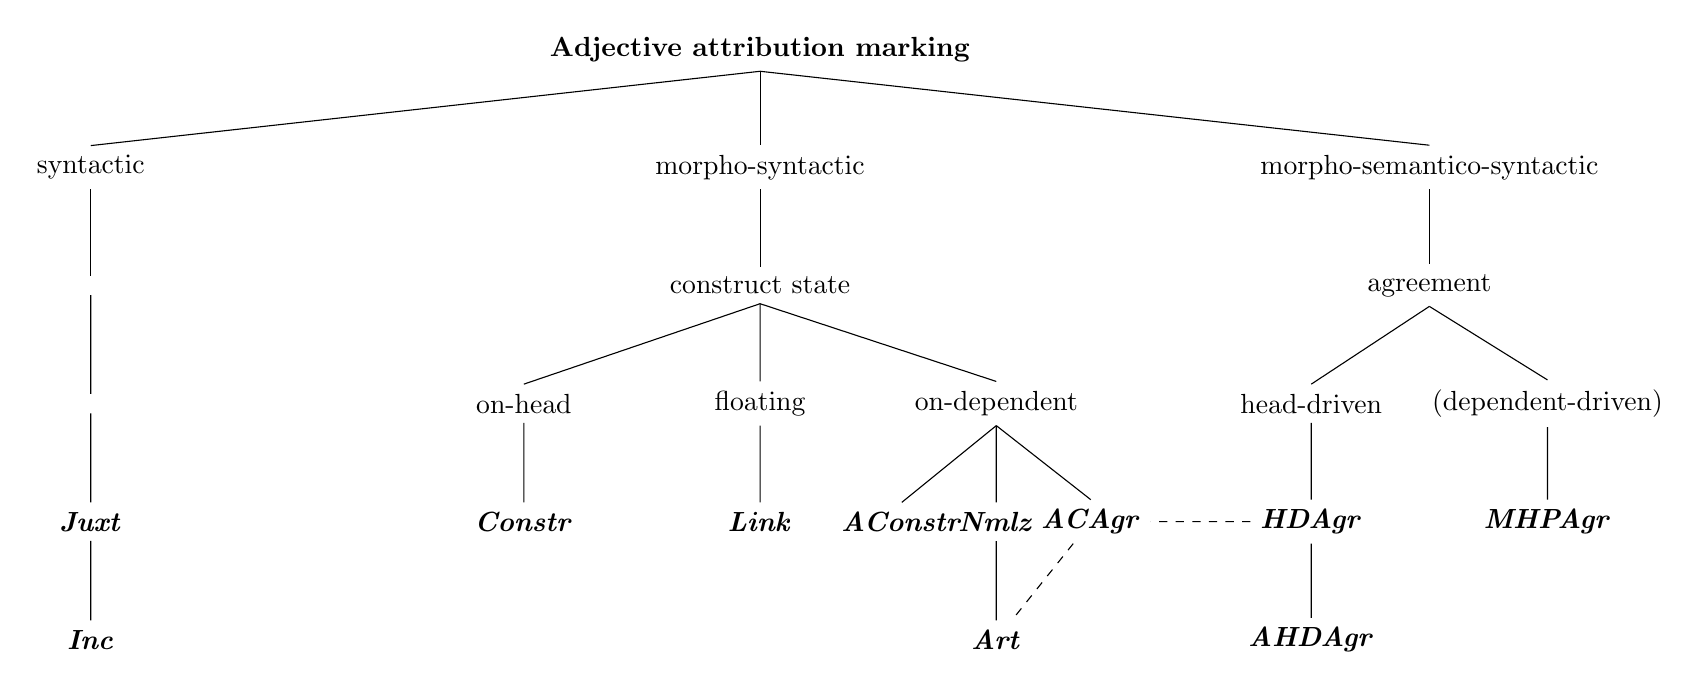
\begin{tikzpicture}
\tikzstyle{level 1}=[sibling distance=85mm]
\tikzstyle{level 3}=[sibling distance=30mm]
\tikzstyle{level 4}=[sibling distance=12mm]
\node {\textbf{Adjective attribution marking}}
child {node {syntactic}
	child {node {}
		child {node {}
			child {node {\textbf{\textit{Juxt}} }
				child {node {\textbf{\textit{Inc}} }
				}
			}
		}
	}
}
child {node {morpho-syntactic}
	child {node {construct state}
		child {node {on-head}
			child{node {\textbf{\textit{Constr}} }
			}
		}
		child {node {floating}
			child{node {\textbf{\textit{Link}} }
			}
		}
		child {node {on-dependent}
			child{node {\textbf{\textit{AConstr}} }
			}
			child{node {\textbf{\textit{Nmlz}} }
				child{node (Art) {\textbf{\textit{Art}} }
				}
			}
			child{node (ACAgr) {\textbf{\textit{ACAgr}} }
			}
		}
	}
}
child {node {morpho-semantico-syntactic}
	child {node {agreement}
		child {node {head-driven}
			child {node (HDAgr) {\textbf{\textit{HDAgr}} }
				child {node {\textbf{\textit{AHDAgr}} }
				}
			}
		}
		child {node {(dependent-driven)}
			child {node {\textbf{\textit{MHPAgr}} }
			}
		}
	}
};
\draw [dashed] (HDAgr) -- (ACAgr) -- (Art);
\end{tikzpicture}
\end{figure}
\end{landscape}

%
\chapter[Polyfunctionality]{Excursus: Polyfunctionality of attribution marking devices} \label{polyfunctionality}
In a typological survey, noun phrases with adjectival modifiers can be examined from different perspectives. In the previous chapter, noun phrases with attributive adjectives were described according to their syntactic, morpho-syntactic, and/or morpho-semantico-syn\-tac\-tic structure. But noun phrase types of a given language can also be defined on a polyfunctionality scale with regard to the class of attributed elements beyond adjective attribution: Attributive adjectives and other adnominal modifiers (such as demonstratives, possessor nouns, adpositional phrases, clauses, etc.) may or may not be used in similar noun phrase structures.

Moreover, polyfunctionality is also relevant in languages where one and the same device is used as a nominal modification marker beyond attribution: for modification inside an adjective phrase (licensing, for instance, a degree word as modifier of an adjective) or as a modification marker inside an adpositional phrase (licensing, for instance, an adposition as determined by a noun phrase). \textit{Attribution marker} should thus be understood as a term denoting a subset of \textit{modification markers} relevant to nominal phrase structure in general.

Finally, the polyfunctionality concerns even the semantic content (or function) of certain devices beyond modification marking. 

In the present chapter, polyfunctionality of adjective attribution marking devices will be illustrated with examples from a few languages.

\section{Polyfunctionality of modification markers}
%check zu possessor compounding Dahl 2004. The growth and maintenance of linguistic complexity. Studies in language companion series, 71. Amsterdam: John Benjamins.
In many languages, more than one class of attributes belong to one and the same noun phrase type. Some languages exhibit even highly polyfunctional noun phrase types and use one and the same device for licensing verbs, nouns, adjectives and even other syntactic classes as attributive modifiers inside noun phrases.

In example (\ref{multi mand}) from Mandarin Chinese, the anti-construct state marker \textit{de} illustrates a highly polyfunctional attribution marking device. It licenses adjectival (\ref{mandarin adj}), nominal (\ref{mandarin noun}) and verbal attributes (\ref{mandarin rel}).\footnote{Note, however, that the attributive marker is not obligatory. In noun phrases with pronominal and adjectival attributes, it can also be omitted. If \textit{de} is used with adjectives, a certain clarifying or delineating stress is put on the denoted property, e.g.~\textit{hóng hūa} [red flower] ‘a red flower’, \textit{hóng de hūa} [RED \textsc{attr} flower] ‘a flower that is red (and not of a different color)’ \citep[119–123]{li-etal1981}.}

\begin{exe}
\ex \textsc{Mandarin Chinese} (Sinitic<Sinotibetan; \citealt{li-etal1981}) \label{multi mand}
\begin{xlist}
\ex	Noun (possessor) attribute \label{mandarin noun}
\gll	Zhāngsān 	\textbf{de} 	shū\\
	Zhangsang 	{\textsc{attr}} 	book\\
\glt	‘Zhangsang's book’
\ex	Adjectival attribute \label{mandarin adj}
\gll	xīn 		(\textbf{de}) 	shū\\
	new	 	({\textsc{attr}}) 	book\\
\glt	‘new book’
\ex	Verbal (relative clause) attribute \label{mandarin rel}
\gll	wŏ zuótiān 	măi 	\textbf{de} 	shū\\
	1\textsc{1sg} 	buy	yesterday 	{\textsc{attr}} 	book\\
\glt	‘the book I bought yesterday’
\end{xlist}
\end{exe}
In Minangkabau, an Austronesian language spoken on Sumatra in Indonesia, juxtaposition is polyfunctional to a similar degree.
\begin{exe}
\ex \textsc{Minangkabau} (Malayan<Austronesian; \citealt[3–4]{gil2005}) \label{multi minangkabau}
\begin{xlist}
\ex Noun (possessor) attribute
\gll	batiak Kairil\\
	papaya Kairil\\
\glt	‘Kairil's papaya’
\ex Adjectival attribute
\gll	batiak kuniang\\
	papaya yellow\\
\glt	‘a/the yellow papaya’
\ex Verbal (relative clause) attribute
\gll	batiak Kairil bali\\
	papaya Kairil buy\\
\glt	‘a/the papaya that Kairil bought’
\end{xlist}
\end{exe}
Tagalog is another language with a polyfunctional attribution marker. The Tagalog linker, however, is less polyfunctional than juxtaposition in Minangkabau or anti-construct state marking in Mandarin Chinese. It marks only verbal and adjectival attributes.\footnote{Note that that the constituent order of attribute and head noun is free in Tagalog: The relative clause and the adjective can also occur in a head-initial phrase type. In this case, the linker \textit{=ng} attaches phonologically to the noun (\citealt[1]{gil2005}; \citealt[160, 162]{himmelmann1997}).}
\begin{exe}
\ex \textsc{Tagalog} (Meso-Philippine<Austronesian; \citealt[6]{gil2005}) \label{multi tagalog}
\begin{xlist}
\ex Adjectival attribute
\gll	pula\textbf{=ng} mangga\\
	red{=\textsc{attr}} mango\\
\glt	‘red mango’
\ex Verbal (relative clause) attribute
\gll	binili ni Jojo\textbf{=ng} mangga\\
	bought \textsc{pers.gen} Jojo{=\textsc{attr}} mango\\
\glt	‘mango that Jojo bought’
\end{xlist}
\end{exe}
Highly polyfunctional attribution marking by means of a head-marking construct suffix is found even in Persian.\footnote{Note the consistent glossing \textsc{mod} instead of \textsc{attr}. The Persian construct marker licenses modification beyond attribution.}
\begin{exe}
\ex \textsc{Persian} (SW-Iranian<Indoeuropean; \citealt{mahootian1997})\label{multi persian}
\begin{xlist}
\ex Modification inside an adpositional phrase
\gll	tu\textbf{-ye} ašpæzxune\\
	in\textbf{-\textsc{mod}} kitchen\\
\glt ‘in the kitchen’
\ex Nominal attribution
\begin{xlist}
\ex Noun (non-possessor) attribute
\gll 	ængoštær\textbf{-e} ælmas\\
	ring-\textsc{mod} diamond\\
\glt 	‘diamond ring’
\ex Noun (possessor) attribute
\gll	ængoštær\textbf{-e} pedær\\
	ring-\textsc{mod} father\\
\glt	‘father's ring’
\end{xlist}
\ex Adjectival attribute
\gll	ælmas\textbf{-e} bozorg\\
	diamond-\textsc{mod} big\\
\glt	‘a big diamond’
\ex Adpositional attribute
\gll	miz\textbf{-e} tu{-ye} ašpæzxune\\
	table-\textsc{mod} in{-\textsc{mod}} kitchen\\
\glt ‘the table in the kitchen’
\ex (Infinite) verbal attribute
\gll	væqt\textbf{-e} ræftæn\\
	time-\textsc{mod} to\_go\\
\glt	‘time to go’
\end{xlist}
\end{exe}
While nominal, adjectival, adpositional and (infinite) verbal attributes are mark\-ed by the same device, finite verbal attributes (relative clauses) never occur in a similar noun phrase type in Persian.

In Västerbotten-Swedish, a language of the northern Eurasian area under investigation, attribution marking by means of adjective incorporation is also considered to be polyfunctional (cf.~Sections \ref{attr incorporation} and \ref{bondska synchr}). Beside adjective attribution, the device marks attribution of (human) possessors.%\cite[5]{gil2005}
\begin{exe}
\ex \textsc{Västerbotten-Swedish} (N-Germanic<Indoeuropean; \citealt[5]{gil2005}) \label{multi bondska}
\begin{xlist}
\ex Noun (human possessor) attribute
\gll	Pelle-äpple\\
	Pelle-apple\\
\glt	‘Pelle's apple’
\ex Adjectival attribute
%\begin{xlist}
%\ex (lexical adjective)
\gll	rö-äpple\\
	red-apple\\
\glt	‘red apple’
%\ex (past participle)
%\gll	(stick-ad)-tröja\\
%	(knitt-\textsc{ptcp:pst})-sweater\\
%\glt	‘knitted sweater’
%\end{xlist}
\end{xlist}
\end{exe}
Gil (\citeyear{gil2005}) surveyed the polyfunctionality of attribution markers licensing possessor nouns, adjectives and relative clauses in a world-wide sample of languages. According to the number of morpho-syntactically differentiated classes of attributes Gil grouped the languages of his sample into the following types:
\begin{itemize}
\item \textbf{Weakly differentiating languages} using polyfunctional devices for attribution of all three syntactic categories, as in Mandarin (\ref{multi mand}) and Minangkabau (\ref{multi minangkabau})
\item \textbf{Moderately differentiating languages} using polyfunctional devices for attribution of two syntactic categories, for instance:
	\subitem – adjectives and relative clauses, as in Tagalog (\ref{multi tagalog})
	\subitem – possessor nouns and adjectives, as in Västerbotten-Swedish (\ref{multi bondska}) and Persian (\ref{multi persian})
\item \textbf{Highly differentiating languages} are not polyfunctional at all, as in German where the three syntactic classes are marked differently.
\end{itemize}
In Gil's sample, Europe and adjacent parts of Asia and Africa stand out as an area with predominantly non-polyfunctional languages, while almost all languages of Southeast Asia are of low differentiation \citep[8]{gil2005}.

Northern Eurasian languages of the “moderately differentiating” type included in Gil's sample are Japanese and Västerbotten-Swedish (with polyfunctional attribution marking of possessor nouns and adjectives) as well as Ainu, Nivkh and Tatar (with polyfunctional attribution marking of adjectives and relative clauses).\footnote{Note that English is not coded as “moderately differentiating” by \citet{gil2005}, although juxtaposition can be polyfunctionally used as a device for attribution of adjectives and relative clauses (with reverse constituent order though: {\it The woman I saw.})} No languages of the “weakly differentiated” type are known to occur in the northern Eurasian area. 

\begin{figure}[htbp] \label{multi abcd}
\begin{center}
\parbox[b]{0.20\textwidth}{
\begin{center}{\sc Mandarin},\\{\sc Minangkabau}\\
\medskip
\begin{tabular}{| c |}
\hline
\\
\hline
\hline
\\
\hline
{\sc attr}_{Rel}\\
\hline
{\sc attr}_{A}\\
\hline
{\sc attr}_{N}\\
\hline
\end{tabular}
\end{center}
}
\parbox[b]{0.20\textwidth}{
\begin{center}{\sc Tagalog}\\
\bigskip
\begin{tabular}{| c |}
\hline
\\
\hline
\hline
\\
\hline
{\sc attr}_{Rel}\\
\hline
{\sc attr}_{A}\\
\hline
\\
\hline
\end{tabular}
\end{center}
}
\parbox[b]{0.20\textwidth}{
\begin{center}{\sc Västerbotten-}\\{\sc Swedish}\\
\medskip
\begin{tabular}{| c |}
\hline
\\
\hline
\hline
\\
\hline
\\
\hline
{\sc attr}_{A}\\
\hline
{\sc attr}_{N}\\
\hline
\end{tabular}
\end{center}
}
\parbox[b]{0.20\textwidth}{
\begin{center}{\sc Persian}\\
\bigskip
\begin{tabular}{| c |}
\hline
{\sc mod}_{NP}\\
\hline
\hline
{\sc attr}_{AdP}\\
\hline
\\
\hline
{\sc attr}_{A}\\
\hline
{\sc attr}_{N}\\
\hline
\end{tabular}
\end{center}
}
\end{center}
\caption[Functional map for modification marking]{Functional maps for modification markers: the anti-construct state marking in \textsc{Mandarin Chinese} and juxtaposition in \textsc{Minangkabau}, the linker in \textsc{Tagalog}, adjective incorporation in \textsc{Västerbotten-Swedish} and construct state marking in {\sc Per\-si\-an}}
\end{figure}

\noindent Figure \ref{multi abcd} illustrates the polyfunctionality of modification markers in the languages mentioned in this chapter.\footnote{Cf.~\cite{haspelmath2003}, for a systematic and historiographic description of functional (or semantic) maps.} The true attributive functions of the marker, i.e.~licensing of adpositional, verbal, and adjectival attributes, are found in the middle cells of the left column in Figure \ref{multi abcd}. The cell extending upwards shows the additional function of the marker as licensee of modification above the noun phrase level (i.e.~inside an adposition phrase).% or below the noun phrase level (i.e.~inside an adjective phrase).

The order of {\sc attr}_{Rel} through {\sc attr}_{N} in these functional maps corresponds to the hierarchical alignment of polyfunctional attribution marking suggested by Bingfu Lu and Zhenglin Qu.\footnote{Lu's and Qu's hierarchy, cited from a LingTyp posting (“The alignment of modification coding”, LingTyp Item \#2580, 6 May 2009, 01:36, \url{http://listserv.linguistlist.org/cgi-bin/wa?A2=ind0905A&L=LINGTYP&P=R146}) is based on a similar hierarchy for Austronesian languages by Foley (\citeyear{foley1980}). Note that Foley's hierarchy is proposed to be cross-linguistically valid and even includes two more syntactic classes than considered here: Determiner > Numeral > Noun > Adjective > Verb.}
\begin{exe}
\ex	Noun < Adjective < Verb
\end{exe}
The hierarchy is to be read as follows: The highest category of attributive modifiers are verbs (i.e.~relative and other attributive clauses), the next lower categories are adjectives and nouns. If one attributive category is marked with a polyfunctional attribution marker, the less bounded category adjacent to the left side in the hierarchy should be marked by the same device, too.

\begin{figure}[htbp]
\parbox[b]{\textwidth}{
\begin{center}
\begin{tabular}{| c || c | c |}
\cline{1-1}
\\
\hline
{\sc attr}_{Rel} & {\sc nmlz} & {\sc foc}\\
\hline
{\sc attr}_{A}\\
\cline{1-1}
{\sc attr}_{N}\\
\cline{1-1}
\end{tabular}
\end{center}
}
\caption[Functional map for modification marking]{Functional map for the modification marker \textit{ve} in \textsc{Lahu}}
\label{lahu funcmap}
\end{figure}

\section[Polyfunctionality and additional content]{Polyfunctionality of modification markers and additional content}
Polyfunctional modification marking devices with semantic content (or function) beyond attribution are also attested in several languages. Lahu is an example of a South\-east Asian language of the “weakly differentiating” type according to Gil's (\citeyear{gil2005}) classification. Syntactically similar to Mandarin Chinese, Lahu exhibits an anti-construct state marker \textit{ve} that licenses adjectival (\ref{lahu adj}), nominal (\ref{lahu noun}) and verbal attributes (\ref{lahu rel}). In addition, the marker \textit{ve} in Lahu is used as nominalizer (\ref{lahu compl}) and as focus marker (\ref{lahu focus}).\footnote{See \citealt{bickel1999} on the “Standard Sino-Tibetan Nominalization pattern” which in some languages include even additional content beyond attribution, nominalization and focus.}
\newpage
\begin{exe}
\ex	\textsc{Lahu} (Loloish<Sinotibetan; \citealt{matisoff1973})
\begin{xlist}
\ex	Attribution
\begin{xlist}
\ex	Adjectival attribute \label{lahu adj}
\gll	dàʔ	\textbf{ve}	ŋâʔ\\
	pretty	\textsc{attr}	bird\\
\glt	‘pretty birds’ (194)
\ex	Noun (possessor) attribute \label{lahu noun}
\gll	Càl\^{ɔ}	\textbf{ve}	\`{ɔ}ha\\
	Jalaw	\textsc{attr}	picture\\
\glt	‘Jalaw's picture’ (141)
\ex	Verbal (relative clause) attribute \label{lahu rel}
\gll	c\'{ɔ}	câ	\textbf{ve}	ŋâʔ\\
	boil	eat	\textsc{attr}	bird\\
\glt	‘birds one boils to eat’ (194)
\end{xlist}
\ex	Additional semantic content
\begin{xlist}
\ex Nominalization (of a complement clause)\label{lahu compl}
\gll	n\`{ɔ}	qôʔ \textbf{ve}	thàʔ	ŋà mâ	na ɣa	qôʔ-ma!\\
	you	say \textsc{NMLZ}	\textsc{acc} I	\textsc{neg} understand	be\_able	\textsc{interj}\\
\glt	‘I can't catch what you're saying!’ (157)
\ex	Focusing (of a clause) \label{lahu focus}
\gll	mâ		qay	\textbf{ve}\\
	\textsc{neg}	go	\textsc{FOC}\\
\glt	‘I am certainly not going.’ (362)
\end{xlist}
\end{xlist}
\end{exe}
The functions of the marker \textit{ve} in Lahu can also be summarized in a functional map, see Figure \ref{lahu funcmap}. The true attributive functions of the marker, i.e.~licensing of verbal, nominal and adjectival attributes, are found in the cells of the left column in Figure \ref{lahu funcmap}. The cells extending to the right show the additional content of the attributive marker, i.e.~as a nominalizer and focus marker of a clause.

\section{Conclusion}
From a purely synchronic point of view, polyfunctionality of adjective attribution marking devices seems less relevant to the area under investigation, northern Eurasia. Most languages of the area exhibit highly differentiated attribution marking devices. Languages of the “moderately differentiating” type are rare; no languages of the “weakly differentiated” type are known to occur in the northern Eurasian area at all.

However, polyfunctionality can perhaps indicate historical change if additional semantic content of attribution marking devices across related languages is taken into consideration. The topic of polyfunctional attribution markers across languages of one family will thus be taken up again in Part \ref{part synchr} of this study.

%%%%%%

\part{Synchrony} \label{part synchr}

%
\chapter{Introduction}
\section{The languages of northern Eurasia}
The geographic area covered in the present survey stretches from Europe (including the Mediterranean Islands Malta and Cyprus as well as the regions Anatolia and Caucasia), over central, northern, and northeastern Asia (including the whole of Siberia, the adjacent parts of northern Mongolia and Manchuria) to the Islands of the northwestern Pacific Ocean. The language families represented in this area are genealogically categorized by \cite{salminen2007} in his chapter on the endangered languages of “Europe and North Asia”. By and large, Salminen's index of languages will be followed here. However, the present survey strictly follows the geography of northern Eurasia and consequently also includes Siberian Yupic Eskimo, Ainu, the Sinotibetan language Dungan, and some Semitic languages.

Adopting Salminen's rather cautious genealogical classification the following families are considered (roughly from Northeast to Southwest):
\begin{itemize}
\item{Eskimo-Aleut}
\item{Chukotkan}
\item{Kamchatkan}
\item{Nivkh}
\item{Ainu}
\item{Japanese}
\item{Korean}
\item{Sinotibetan}
\item{Mongolic}
\item{Tungusic}
\item{Yukagir}
\item{Yeniseian}
\item{Turkic}
\item{Nakh-Daghestanian}
\item{Abkhaz-Adyge}
\item{Kartvelian}
\item{Semitic}
\item{Uralic}
\item{Indoeuropean}
\item{Basque}
\end{itemize}
Even though some of these genealogical units have been assumed to combine to larger stocks (as Altaic, Chukotko-Kamchatkan, North-Caucasian and other) the restriction to uncontroversial units seems adequate for the present areal typological investigation. This is especially true since an attempt is made to map variation inside genealogical units rather than to evaluate a statistically balanced genealogical sample of languages.

\section{The language sample}
All attested adjective attribution marking devices of languages mentioned in the present study are coded in Table \ref{sample} in the appendix.\footnote{The table is derived from \citet{AUTOTYP-NP} where these languages are coded for noun phrase patterns.} This table thus includes a relatively complete list of languages from the northern Eurasian area. At least one representative of each existing genera is found in that sample. Additionally, several languages from within or outside the area (all of which are mentioned in other chapters of this investigation) or even other languages on which information was easily accessible are coded.

All languages are sorted alphabetically according to their genealogical affiliation. For each of the languages, the attested noun phrase type(s) relevant to adjective attribution marking are listed.

\section{The language maps}
\subsection[Geographic coding]{Data points: geographic coding}
The language maps have been generated using the interactive reference tool 
for the World Atlas of Language Structures \citep{bibiko2005}. Each language is displayed as one data point. The respective geographic coordinates have either been taken from \cite{WALS} or were included using the language coordinates provided by \cite{AUTOTYP} or on Ljuba Veselinova's website.\footnote{\url{http://www.ling.su.se/staff/ljuba/}} For some languages missing in the mentioned databases new coordinates had to be defined based on the main geographic location where the respective languages are spoken.

Displaying the distribution of a given feature by means of a borderline around a group of languages – as in the maps used by typological surveys of the EUROTYP-project\footnote{\url{http://www-uilots.let.uu.nl/ltrc/eurotyp/index.htm}} – was not preferred because these maps might imply the existence of isoglosses around continuous language and dialect areas. A typological survey of non-continous languages seems rather inadequate for drawing such isoglosses.\footnote{Cf.~also Van Pottelberge's \citeyear{van-pottelberge2001} critique of EUROTYP's “name maps”. Furthermore, the Eurotyp sample of languages are somewhat arbitrary. The western Romance varieties, for instance, are represented in large number whereas varieties of Balkan Romance (Megleno-Rumanian, Aromunian, etc.) are missing completely. Also the whole Saamic branch is represented in the Eurotyp sample as one single language only even though Saamic languages are as comparably diverse as Romance languages.}

\subsection[Type coding]{Data points: type coding}
%Farben markieren verschiedene Typen
%Formen markieren Untertypen (secondary types)
In several languages more than one default attribution marking device occurs, for example in Albanian (cf.~chapter \ref{albanian synchr}) where two lexical classes of adjectives exist: one of them marked for head-driven agreement, the other simultaneously marked for head-driven agreement and attributive nominalization. In the map's legend, a slash marks the occurrence of multiple basic types in one language: \textsc{Albanian} \textit{HDrAgr/Nmlz+HDrAgr}.\footnote{Type abbreviations are explained in Table \ref{sample} in the appendix.}

Parentheses denote secondary types of attribution marking devices with additional semantic content, as Chuvash (cf.~chapter \ref{chuvash synchr}) where attributive adjectives are normally juxtaposed but can alternatively be marked for attributive nominalization in contrastive-focus constructions: \textsc{Chuvash} \textit{Juxt(Nmlz)}.

Square parenthesis will be used for languages where the occurrence of a given type of attribution marking devices seems even more restricted or if the device's characteristics remain uncertain due to inadequate data. Consider for example Turkish (cf.~chapter \ref{turkish synchr}) where attributive nominalization occurs as a secondary type but is restricted to headless noun phrases in direct object position (marked for accusative): \textsc{Turkish} \textit{Juxt[Nmlz]}. 
Secondary and tertiary types are not coded in the maps. 

\subsection{The maps}
Maps \ref{WorldMap} and \ref{WorldMapTyp} show the distribution of different adjective attribution marking devices across those world's languages mentioned in the present study. Whereas all types are coded with different colors or shapes in Map \ref{WorldMap}, a similar language sample is coded only for the main morpho-syntactic types (juxtaposition, agreement, construct state, incorporation) in Map \ref{WorldMap}. Note that these world maps do not reflect systematic sampling but are rather the result of random choice due to my work with data coded for the noun phrase structure module of AUTOTYP \citep{AUTOTYP-NP}. Note also that the maps show fewer languages from the northern Eurasian area than actually coded in Table \ref{sample}.

The other pairs of maps are coded similarly but zoom in on northern Eurasia (Maps \ref{NEMap} and \ref{NEMapTyp}), on North-Asia (Maps \ref{NAMap} and \ref{NAMapTyp}) and on Europe (Maps \ref{EUMap} and \ref{EUMapTyp}). Whereas the maps of northern Eurasia and North-Asia show only representatives of each genera, the maps of Europe present a more complete picture. The reason for displaying a deeper resolution in the European map is the easier accessibility of data for almost all existing languages of that area. Displaying a similar deep resolution on the whole northern Eurasian area was not possible due to lack of data for several languages.

In order to present a balanced picture, several European languages are thus not displayed in the larger map of northern Eurasia. When a choice had to be made whether or not to keep a language inside a given genera, this was always done in favor of diversity rather than unity. One genera can even be represented by more than one language in order to display extraordinary diversity inside that group of closely related languages. Consequently, the northern branch of Germanic is represented by Icelandic (with \textit{HDrAgr}), Swedish (with \textit{ACAgr+HDrAgr/HDrAgr}) and Västerbotten-Swedish (with \textit{Inc/HDrAgr}) (cf. Section \ref{n-germanic synchr}).

The choice to let the maps illustrate the highest possible diversity instead of displaying a genealogically and geographically balanced picture is legitimated by the general goal of the present investigation, namely the synchronic and diachronic mapping of cross-linguistically attested adjective attribution marking devices in a geographically restricted area. Whereas the mapping of synchronically attested diversity is the aim of the present part, Part \ref{part diachr} will inspect this diversity form a diachronic perspective.

%
\chapter[The languages of northern Eurasia]{Adjective attribution marking in the languages of northern Eurasia}

The following chapter contains an overall survey of adjective attribution marking devices which occur in the languages of northern Eurasia. For each genealogical unit, both the prototypical and the known minor noun phrase type(s) will be characterized and illustrated with examples. A complete list of adjective attribution marking devices in over 200 single languages considered for the present survey is found in Table \ref{sample} starting on page \pageref{sample} in the appendix. The geographic spread of the different noun phrase types is shown on several Maps starting on page \pageref{WorldMap} in the appendix.

\section{Eskimo-Aleut}
\subsection{Eskimo}
\subsubsection{Yupic}
Whereas most languages of the Eskimo-Aleut family are spoken on islands in the Bering Strait or on the North American continent, a few varieties of the Yupik subbranch of Eskimo can be localized to north-easternmost Siberia. But only one of these languages, Central Siberian Yupic, is still spoken \cite[224]{salminen2007}.

In Central Siberian Yupic, only one adjective attribution marking device is attested:
\begin{itemize}
\item Incorporation.
\end{itemize}

\paragraph{Adjective incorporation in Central Siberian Yupic}
Property words (“adjectives”) in Central Siberian Yupic are phonologically bound nominal roots. Adjectival modification is thus expressed by means of polysynthetic morphology and can be characterized as adjective incorporation according to the ontology presented in Part \ref{part typ}.
\begin{exe}
\ex \textsc{Central Siberian Yupic} \citep{de-reuse1994}
\begin{xlist}
\ex
\gll	qawaagpag\textbf{-rukutaagh-\underline{gh}llag}-Ø\\
	legendary\_large\_bird-huge.\textsc{noun}-big.\textsc{noun}-\textsc{abs}\\
\glt	‘huge big (legendary large) bird’ (54)
\ex	
\gll	mangteghagh\textbf{-\underline{gh}llag}-lgu-uq\\
	house-big.\textsc{noun}-have.\textsc{noun}-\textsc{ind}(3s)\\
\glt	‘He has a large house.’ (55)
\ex	
\gll	mangteghagh\textbf{-\underline{gh}rugllag}-ngllagh-yug-nghit°e-unga\\
	house-big.\textsc{noun}-make.\textsc{noun}-want\_to.\textsc{verb}-\textsc{neg}-\textsc{ind(1s)}\\
\glt	‘I did not want to make a large house.’ (56)
\end{xlist}
\end{exe}

\section{Chukotkan}
The Chukotkan language family (aka Chukchi-Koryak) consists of two bran\-ches. The first branch, Chukchi, is represented by only one language, Chukchi, which has the same name as the branch itself. The second branch, Koryak, is represented by the two languages Alutor and Koryak. A third branch, Kerek, is probably extinct \cite[253]{salminen2007} and consequently not considered here.\\

\noindent Constituent order inside the noun phrase of Chukotkan languages is strictly head-final. Adjective attribution marking is also similar in all Chukotkan languages. Two types are attested:
\begin{itemize}
\item Incorporation
\item Head-driven agreement.
\end{itemize}

\subsection{Chukchi}
\paragraph{Adjective incorporation in Chukchi}
The use of the bound adjective morpheme in the polysynthetic structure (similar to Yupic) is illustrated in the following examples.\footnote{The vowel -ə- in these and the following examples is epenthetic.}

\begin{exe}
\ex \textsc{Chukchi} \citep{skorik1960}
\begin{xlist}
\ex	
\gll	\textbf{elg-}ə-qoranə\\
	white-ə-deer:\textsc{abs.sg}\\
\glt	‘white reindeer’
\ex
\gll	\textbf{elg-}ə-qorat\\
	white-ə-deer:\textsc{abs.pl}\\
\glt	‘white reindeer (pl)’
\end{xlist}
\end{exe}

\subsection{Koryak}
\paragraph{Adjective incorporation in Alutor}
Similar to Chukchi, adjective incorporation is the default adjective attribution marking device in Alutor.
\begin{exe}
\ex \textsc{Alutor} \citep{nagayama2003}
\begin{xlist}
\ex
\gll	\textbf{meŋ-}ə-rara-ŋa\\
	big-ə-house-\textsc{abs.sg}\\
\glt	‘large house’
\ex
\gll	\textbf{meŋ-}ə-rara-wwi\\
	big-ə-house-\textsc{abs.pl}\\
\glt	‘large houses’
\end{xlist}
\end{exe}

\paragraph{Head-driven agreement in Chukchi and Alutor}
Whereas adjective incorporation is the default and unmarked type of adjective attribution marking in Alutor and Chukchi, several descriptions of the Chukotkan languages mention that adjectives can also occur in an unbound form (for Alutor \citealt{nagayama2003}; for Chukchi \citealt[103–104, 421–429]{skorik1960}, \citealt[251]{comrie1981}). As unbound morphemes adjectives take the stative marker \textit{n-} as well as agreement markers for person, number and case.
\begin{exe}
\ex \label{chukchi alutor free adj}
\begin{xlist}
\ex \textsc{Chukchi} \citep{skorik1960}
\begin{xlist}
\ex
\gll	\textbf{n-ilg-ə-qin-Ø} qoranə\\
	\textsc{stat}-white-ə-\textsc{3sg} deer:\textsc{abs.sg}\\
\glt	‘white reindeer’
\ex
\gll	\textbf{n-ilg-ə-qine-t} qorat\\
	\textsc{stat}-white-ə-3-\textsc{pl} deer:\textsc{abs.pl}\\
\glt	‘white reindeer (pl)’
\end{xlist}
\ex \textsc{Alutor} \citep{nagayama2003}
\begin{xlist}
\ex
\gll	\textbf{n-ə-meŋ-ə-qin} rara-ŋa\\
	\textsc{stat}-ə-big-ə-\textsc{abs:3sg} house-\textsc{abs.sg}\\
\glt	‘large house’
\ex
\gll	\textbf{n-ə-meŋ-ə-laŋ} rara-wwi\\
	\textsc{stat}-ə-big-ə-\textsc{abs:3pl} house-\textsc{abs.pl}\\
\glt	‘large houses’
\end{xlist}
\end{xlist}
\end{exe}
The number/person/case-agreement suffixes of adjectives and the suffixes mar\-king possessive inflection of nouns belong to one and the same para\-digm. Consequently, one could also interpret the Alutor and Chukchi data as another instance of modifier-headed possessor agreement (as in Oroch described in Section \ref{ModheadAgr}). If so, the examples in (\ref{chukchi alutor free adj}) should be translated literally as ‘reindeer's whiteness’, ‘house's bigness’. An analysis against syntactic head shift between noun and adjective, however, is preferred here for two reasons: The first reason is the constituent order inside the noun phrase. The assumed head shift to a modifier-headed possessor agreement construction would violate the otherwise strictly head-final constituent order rule in Alutor and Chukchi. 

The other reason for arguing against syntactic head shift between noun and adjective is that in order to use non-incorporating constructions as in the examples in (\ref{chukchi alutor free adj}) the adjective is first transformed into a stative verb by means of a verbalizing prefix (\textit{-n}, glossed as \textsc{stat} in example \ref{chukchi alutor free adj}).

The verbalizer together with the agreement affix is sometimes glossed as an adjectivizing circumfix (\textsc{adjz>-\dots-<adjz:agr}), for instance in Nagayama's (\citeyear{nagayama2003}) grammatical description of Alutor. The given noun phrase type should then perhaps be analyzed as attributive state marking (as in Russian, see Sections \ref{anti-constr agr} and \ref{russian synchr}). Unlike in Russian, however, the same agreement marking as in attributive constructions shows up on predicates as well.
\begin{exe}
\ex \textsc{Alutor} \citep{nagayama2003}
\begin{xlist}
\ex
\gll	{\bf n-ə-tur-}iɣəm\\
	\textbf{\textsc{stat}-ə-young-}\textsc{1sg}\\
\glt	‘I'm young’
\end{xlist}
\end{exe}
Consequently, an analysis of adjective attribution marking in Alutor and Chuk\-chi as belonging to the state marking type is rejected.

The semantic difference between the two constructions, with adjective incorporation on the one hand hand and head-driven agreement marking on the other hand, is not clear. Whereas adjective incorporation is often described as the main or even only possible type (for Chukchi cf.~\citealt[37, 101]{kampfe-etal1995}), \citet[288]{kibrik-etal2000} states that this type indicates the corresponding quality or property as referring to background information in Alutor.

The following example from Chukchi on the other hand, indicates that the non-incorporated adjective is used in an emphasized construction. Sentence (\ref{chukchi free adj}) was elicited in order to find examples of multiple modifiers in one noun phrase, which seems to be avoided by speakers of Chukchi \cite[330]{rijkhoff2002}. In sentence (\ref{chukchi inc adj}) with the incorporated adjective, the speaker simply left out the demonstrative when translating into Chukchi.
\begin{exe}
\ex \textsc{Chukchi} \cite[330]{rijkhoff2002}
\begin{xlist}
\ex \label{chukchi free adj}
\gll	əngena-t ngəroq \textbf{n-ilg-ə-qine-t} qora-t\\
	this-\textsc{pl} three \textsc{stat}-white-ə-3-\textsc{pl} deer-\textsc{pl}\\
\glt	‘these three white reindeer’
\ex \label{chukchi inc adj}
\gll	ətlon ga-twetcha-twa-len ga-ngəron-\textbf{elg-}ə-qaa-ma\\
	\textsc{3sg} \textsc{pfct}-stand\_up-be-\textsc{3sg} \textsc{com}-white-ə-deer-\textsc{com}\\
\glt	‘He stood next to (these) three white reindeer.’
\end{xlist}
\end{exe}
\citet[716]{bogoras1922} states that the circum-positioned marker of the unbound adjective “sometimes corresponds to the definite article or designates an object as referred to before.” The unbound adjective, on the other hand, can only occur in absolute case which is inherently connected to semantic definiteness \citep[cf.][207, elsewhere]{dunn1999}.


\section{Kamchatkan}
The only surviving member of the Kamchatkan language family is Itelmen (aka Western Kamchadal) \citep[224]{salminen2007}.

The only attested type of adjective attribution marking in Itelmen is:\footnote{According to Volodin (\citeyear{volodin1997}) a few adjectives (among them Russian loan adjectives) occur in juxtaposition.}
\begin{itemize}
\item Anti-construct state agreement.
\end{itemize}

\paragraph{Anti-construct state agreement marking in Itelmen} \label{itelmen synchr}
Constituent order inside the noun phrase of Itelmen is head-final. Adjectives form a class syntactically clearly distinguished from nouns: unlike the latter, adjectives are never represented by their root morphemes alone. Unlike verbs, which take TAM markers, adjectives take adjectival morphology and are licensed either by an attributive or predicative (adverbal) suffix (\citealt{volodin1997}, \citealt[54]{georg-etal1999}).
\begin{exe}
\ex \textsc{Itelmen} \citep{volodin1997} \label{itelmen ex}
\begin{xlist}
\ex Attributive state of adjectives
\gll	thun\textbf{-lah}\\
	dark-\textsc{attr}\\
\glt	‘dark’
\ex Predicative state of adjectives
\gll	thun\textbf{-k}\\
	dark-\textsc{pred}\\
\glt	‘(is) dark’
\end{xlist}
\end{exe}
Since attributive adjectives also agree in case (though restricted to instrumental case), the noun phrase type can be characterized as anti-construct state agreement, structurally similar to the type found in Russian. Consider the following example.\footnote{Note that the shape of the state marking suffix \textit{-lan'ļ} ($\leftarrow$ \textit{-lah-ļ}) is the result of a regular morpho-phonological process \citep{georg-etal1999}.}

\begin{exe}
\ex Anti-construct state agreement in \textsc{Itelmen} \cite{georg-etal1999}
\gll	Kəmma çasit t'-nu-qz-al-kiçen \textbf{teŋ-lan'ļ} \textbf{thalthe-ļ}, min kn-anke t-zapasa-qzo-çen.\\
	\textsc{1sg} now \textsc{1sg}>-eat-\textsc{ipfv-fut-<1sg} good-\textsc{attr:ins} meat-\textsc{ins} \textsc{rel} \textsc{1sg-dat} \textsc{1sg}-keep-\textsc{ipfv-3sg-prtc}\\
\glt	‘Now I will eat the good meat which I kept for you.’
\end{exe}

\section{Nivkh}
Nivkh (aka Gilyak) is an isolated language spoken in the far east on the Eurasian continent on Sakhalin Island (Russia) \citep[222–223]{salminen2007}.

The only type of adjective attribution marking attested in Nivkh is:
\begin{itemize}
\item Head-driven agreement.
\end{itemize}

\paragraph{Head-driven agreement in Nivkh}
\noindent Property words in Nivkh are verbal roots. As modifiers in noun phrases these adjectival verbs occur to the left of the head noun in a construction which is sometimes described as a polysynthetic structure (cf.~\citealt[16]{gruzdeva1998}; \citealt[80]{jakobson1971}, quoted by \citealt[138]{rijkhoff2002}). The reason for analyzing adjectives in Nivkh as being incorporated into the modified noun is the phonological boundedness of the constituents evidenced by regular alternations in the initial segments of the noun stem \cite[16]{gruzdeva1998}.
\begin{exe}
\ex \textsc{Nivkh} \citep[16]{gruzdeva1998}
\begin{xlist}
\ex tu ‘lake’
\ex 
\gll	pily-du\\
	be\_big-lake\\
\glt	‘large lake’
\end{xlist}
\end{exe}
In her sketch grammar of Nivkh, however, \cite{gruzdeva1998} glosses adjectival words consequently as morphologically unbound words.\footnote{For instance \textit{čuz pitɣy-Ø} [new book-\textsc{nom}] (19), \textit{kyla n'iɣvn̦} [high man] (33), \textit{pila eri} [big river] (38).}

Interestingly, the phonological stem alternation rules also apply to the plural inflection of nouns and their adjectival attributes by means of reduplication. Thus, in (\ref{nivkh redup}), the reduplicated stem of the participle \textit{m'osk̦} ‘destroyed’ is realized as \textit{-zosk̦} and the reduplicated stem of the noun \textit{mu} ‘boat’ is realized as \textit{-ɣu}.\footnote{Note that initial nasals, as in the noun stem \textit{mu} bound to the adjective in (\ref{nivkh unaltered}) do not alternate.}

\begin{exe}
\ex \textsc{Nivkh} (Gruzdeva pc) \label{nivkh redup}
\begin{xlist}
\ex 
\gll	tuin \textbf{t'osq-mu} hum-d'\\
	here break.\textsc{ptcp}-boat be-\textsc{ind}\\
\glt	‘there is a destroyed boat here’ 
\ex	\label{nivkh unaltered}
\gll	tuin \textbf{t'osq\textasciitilde zosk̦-mu\textasciitilde ɣu} hum-d'[-ɣu]\\
	here break.\textsc{ptcp}-\textsc{pl}-boat-\textsc{pl} be-\textsc{ind}[-\textsc{pl}]\\
\glt	‘there are destroyed boats here’
\end{xlist}
\end{exe}
Note that the number agreement of the attributive forms of adjectives by means of reduplication seems to be archaic. According to Gruzdeva (pc), attributive adjectives practically never reduplicate any more. Examples of reduplicating adjectives are, however, included in the grammar of Panfilov (\citeyear{panfilov1965}).

\section{Ainu}
Ainu is an isolate spoken on Hokkaido Island in northern Japan.

The only type of adjective attribution marking attested in Ainu is:
\begin{itemize}
\item Juxtaposition.
\end{itemize}

\paragraph{Juxtaposition in Ainu}
\label{ainu synchr}
Ainu does not exhibit morphological differences between adjectives and verbs \citep[27]{refsing1986}. Words expressing states (\ref{ainu state}) or properties (\ref{aini qual}) in Ainu are best described as stative verbs. They form a subclass of intransitive verbs and are only semantically distinguished from verbs denoting an action \cite[141–142]{refsing1986}. As modifiers of a noun these property words are juxtaposed to the left.
\begin{exe}
\ex \textsc{Ainu (Shizunai dialect)} \cite[142]{refsing1986}%CHECK PAGES
\begin{xlist}
\ex “State adjective” \label{ainu state}
\gll	\textbf{mokor} cep\\
	sleep fish\\
\glt	‘a sleeping fish’
\ex “Quality adjective” \label{aini qual}
\gll	\textbf{pirka} cep\\
	be\_good fish\\
\glt	‘a fine fish’
\end{xlist}
\end{exe}

\section{Japanese}
The noun phrase structure in Japanese, an isolated language, is strictly head-final. Two types of adjective attribution marking devices are attested:
\begin{itemize}
\item Juxtaposition
\item Anti-construct state marking.
\end{itemize}

\paragraph{Juxtaposition in Japanese}
Two distinct lexical classes of words describe the state that an entity is in. Verbal adjectives belong to the first class. These adjectives are distinguished from stative verbs by the adjectivizer suffix \textit{-i}. Used as predicates, the adjectivized verbs marked with \textit{-i} follow the noun but do not require any copula. Attributive adjectives, on the other hand, are juxtaposed to the left of the modified noun. 

\begin{exe}
\ex Verbal adjectives in \textsc{Japanese} \citep[170]{backhouse1984}
\begin{xlist}
\ex Adjective predication 
\gll	kona rombun-wa \textbf{naga-i}\\
	this article-\textsc{top} long-\textsc{adjz}\\%check gloss ?PRES
\glt	‘This article is long.’
\ex Adjective attribution
\gll	\textbf{naga-i} rombun\\
	long-\textsc{adjz} article\\
\glt	‘long article’
\end{xlist}
\end{exe}
Since the adjectivizer suffix \textit{-i} simply derives adjectives from stative verbs and marks both predicates and attributes it is not considered an attribution marking device. Hence, the class of verbal adjectives in Japanese is merely attributed by juxtaposition. Word order is crucial for differentiating attributive from predicative adjectives. 

\paragraph{Anti-construct state marking in Japanese}
Unlike “verbal adjectives”, which were described in the previous section, the few members of the second adjectival sub-class, i.e.~“nominal adjectives” require a special attributive form marked by the invariable attributive suffix \textit{-na}. 

\begin{exe}
\ex \textsc{Japanese} \citep[72-81]{pustet1989}%REF stimmt nicht
\begin{xlist}
\ex Attribution: verbal adjective
\gll	\textbf{waka-i} hito\\
	young-\textsc{adjz} person\\
\glt	‘a young person’
\ex Attribution: nominal adjective
\gll	\textbf{kiree-na} hito\\
	beautiful-\textsc{attr} person\\
\glt	‘a beautiful person’
\end{xlist}
\end{exe}
Note that the word class boundary between nominal adjectives and nouns in Japanese is not always clear because some words take either the noun attribution marker \textit{-no} (\ref{japan na}) or the adjective attribution marker \textit{-na} (\ref{japan no}) when modifying a noun. The arbitrary behavior of attribution marking of nouns and nominal adjectives in Japanese indicates the continuous nature of these two word classes in this language \citep[79-80]{pustet1989}.

\begin{exe}
\ex \textsc{Japanese} \citep[72-81]{pustet1989}%REF stimmt nicht
\begin{xlist}
\ex Noun attribution \label{japan na}
\gll	\textbf{wazuka-na} okane\\
	little-\textsc{attr} money\\
\glt	‘little money’
\ex Adjective attribution \label{japan no}
\gll	\textbf{wazuka-no} okane\\
	little-\textsc{attr} money\\
\glt	‘little money’
\end{xlist}
\end{exe}

\section{Korean}
Korean is an isolated language spoken on the Korean peninsula in northeastern Asia. The only type of adjective attribution marking attested in Korean is:
\begin{itemize}
\item Anti-construct state marking.
\end{itemize}
Note, however, that Korean does not have a distinct class of adjectives but adjectival notions are expressed by verbs.

\paragraph{Anti-construct state marking in Korean}
The constituent order in the noun phrase of Korean is strictly head-final. Modifying “property words” are verbs equipped with a special attributive suffix \textit{-(u)n} \citep{martin-etal1969}.
\begin{exe}
\ex \textsc{Korean} \citep[61]{chang1996}
\begin{xlist}
\ex
\begin{xlist}
\ex
\gll	i \textbf{ppalka-n} chayk\\
	this be\_red-\textsc{attr} book\\
\ex	
\gll	i \textbf{ppalka-n} chayk i\\
	this be\_red-\textsc{attr} book \textsc{subj}\\
\glt	‘this red book’
\end{xlist}
\ex
\begin{xlist}
\ex	
\gll	ce \textbf{khu-n} namwu\\
	that be\_big-\textsc{attr} tree\\
\ex
\gll	ce \textbf{khu-n} namwu lul\\
	that be\_big-\textsc{attr} tree \textsc{obj}\\
\glt	‘that big tree’
\end{xlist}
\end{xlist}
\end{exe}

\section{Sinotibetan}\label{sinotibetan synchr}
\subsection{Sinitic}
\subsubsection{Chinese}
The Sinotibetan language family is represented in northern Eurasia only by one language, Dungan (aka Dunganese), which is a Gansu variety of Northern Chinese spoken in the Kyrgyz Republic in Central Asia (cf.~\citealt[85]{yuo2003}, \citealt{kalimov1968}).\\

\noindent Two types of adjective attribution marking are attested in Dungan:
\begin{itemize}
\item Juxtaposition
\item Attributive nominalization.
\end{itemize}

\paragraph{Juxtaposition in Dungan}
Adjective attribution marking in the unmarked noun phrase in Dungan is characterized by juxtaposition. Hereby, the adjective either precedes or follows the noun.
\begin{exe}
\ex \textsc{Dungan} \cite[480]{kalimov1968} \label{dungan juxtap}
\begin{xlist}
\ex 	
\gll	\textbf{da} fonzy\\
	big house\\
\ex
\gll	fonzy \textbf{da}\\
	house big\\
\glt	‘large house’
\end{xlist}
\end{exe}

\paragraph{Attributive nominalization in Dungan}
A second noun phrase type with the adjectival modifier marked by a suffix \textit{-di\textsuperscript{1}} occurs in Dungan as well. Whereas juxtaposition constitutes the general and unmarked type of adjective attribution marking, the nominalization device seems to be much more restricted and occurs for example in connection with a comparative (\ref{dungan compattr}) or negated attribute (\ref{dungan negattr}).
\begin{exe}
\ex \textsc{Dungan}
\begin{xlist}
\ex Negated attribute \cite[80]{zevachina2001} \label{dungan negattr}
\gll	gubuə\textsuperscript{3} bu\textsuperscript{1} \textbf{da\textsuperscript{3}-di\textsuperscript{1}} gun\textsuperscript{1}fu\textsuperscript{1}\\
	went \textsc{neg} big-\textsc{attr} time\\
\glt	‘Not much (lit. ‘not big’) time passed.’
\ex Comparative attribute \cite[480]{kalimov1968} \label{dungan compattr}
\gll	\textbf{da-ščer-di} fonzy\\
	bigger-\textsc{compar}-\textsc{attr} house\\
\glt	‘a somewhat larger (i.e.~different) house’\footnote{Note that the quoted transcriptions of the two authors differ from each other.}
\end{xlist}
\end{exe}	
The marker \textit{-di\textsuperscript{1}} is clearly cognate with the functionally similar nominalizer \textit{-de} in Mandarin Chinese (cf.~Example \ref{multi mand} in Section \ref{polyfunctionality}). In Dungan, however, \textit{-di\textsuperscript{1}} is sometimes also described as a marker of predicative adjectives, as in (\ref{dungan emphpred}).
\begin{exe}
\ex	Attributive nominalization in \textsc{Dungan} \cite[82]{zevachina2001}
\label{dungan emphpred}
\gll	ž̨y\textsuperscript{3}gə\textsuperscript{1} mə\textsuperscript{1}mə\textsuperscript{2} \textbf{gan\textsuperscript{1}-di\textsuperscript{1}}\\
	this bread stale-\textsc{attr}\\
\glt	‘This bread is STALE (i.e.~different).’
\end{exe}
\citet[82]{zevachina2001} labels the function of the marker as an “emphasizing-predicative”. But looking at her other examples it becomes obvious that \textit{-di\textsuperscript{1}} does not mark predicative adjectives but rather nominalized attributive adjectives.
\begin{exe}
\ex Attributive nominalization in \textsc{Dungan} \cite[82]{zevachina2001}
\gll	ž̨y\textsuperscript{3}gə\textsuperscript{1} fu\textsuperscript{1} bu\textsuperscript{1}cy\textsuperscript{1} \textbf{xun\textsuperscript{1}-di\textsuperscript{1}}, \textbf{zy\textsuperscript{2}-di\textsuperscript{1}}\\
	this book \textsc{neg} red-\textsc{attr} bordeaux-\textsc{attr}\\
\glt	‘This book is not RED, but BORDEAUX.’\\
	(lit. ‘This book is not a red one, but a bordeaux one.’)
\end{exe}
The nominalizing function of the suffix is also described by \cite{kalimov1968}.
\newpage
\begin{exe}
\ex Attributive nominalization \textsc{Dungan} \cite[484]{kalimov1968} \label{dungan nmlz}
\gll	\textbf{ščin-di} gǔjdixyn\\
	new-\textsc{attr} expensive\\
\glt	‘The new (one) is expensive.’
\end{exe}
Attributive marking with the suffix \textit{-di\textsuperscript{1}} in Dungan needs to be investigated in more detail, especially in connection to word order. The head-initial structure seems to be used in order to emphasize the property denoted by the adjective.

However, according to the descriptions of Dungan taken into account here (i.e.~\citealt{kalimov1968} and \citealt{zevachina2001}), the language exhibits two adjective attribution marking devices: juxtaposition and attributive nominalization by means of the article \textit{-di\textsuperscript{1}}. While juxtaposition (with the order adjective-noun) seems to be the unmarked type, attributive nominalization is restricted to certain pragmatically marked constructions.

\section{Mongolic}
%Mongolic-nördliches China: Dagurisch, Mongorisch, Bao'an, Donxiang, Oirat
The Mongolic language family consists of five branches (cf.~\citealt[222]{salminen2007}): The core branch, Mongolian, includes the languages Kalmyk, Khalkha, Khamnigan Mongol, and Oyrat (aka Oirat). Kalmyk is spoken in easternmost Europe (in the Republic of Kalmykia of the Russian Federation). The other Mongolian languages are all spoken in Central Asia, along with Dagur which belongs to a satellite branch of the Mongolic family. Languages of the remaining 3 satellite branches of Mongolic are not considered here since they are all spoken outside the northern Eurasian area.\\
				
\noindent With regard to their principal noun phrase structure, all Mongolic languages of northern Eurasia exhibit the inherited proto-Mongolian features, including strictly head-final word order and juxtaposition of attributive adjectives (“adjecti\-val nouns”) as the only attribution marking device.

Note, however, that adjectives in Mongolic languages do not differ formally from regular nouns but are distinguishable from the latter only by their syntactic behavior and specific derivational patterns (cf.~\citealt[10]{janhunen2003b} for proto-Mongolic and \citealt[161]{svantesson2003} for Khalkha).\footnote{In the two Mongolic languages Moghol (spoken in Afghanistan) and Mangghuer (spoken in China) there is a distinct class of adjectives (cf.~\citealt[252]{weiers2003} for Moghol and \citealt[311]{slater2003} for Mangghuer). However, these languages are not considered since they are spoken outside the northern Eurasian area.}\\

\noindent The only type of adjective attribution marking attested in Mongolic languages of northern Eurasia is:
\begin{itemize}
\item Juxtaposition.
\end{itemize}

\subsection{Mongolian}
\paragraph{Juxtaposition in Khalkha}
The only attested adjective attribution marking device in the languages of the Monguor branch of Mongolic is \textbf{juxtaposition}, similar to the following example. 
\begin{exe}
\ex \textsc{Khalkha} \citep{svantesson2003} \label{khalkha juxt}
\begin{xlist}
\ex
\gll	sayin nom\\
	good book\\
\glt	‘good book’
\ex 
\gll	sayin nom-uud\\
	good book-\textsc{pl}\\
\glt ‘good books’
\end{xlist}
\end{exe}

\subsection{Monguor}
The only attested adjective attribution marking device in the languages of the Monguor branch of Mongolic is \textbf{juxtaposition} \citep{slater2003}, similar to example (\ref{khalkha juxt}) from Khalkha Mongolian.

\subsection{Moghol}
The only attested adjective attribution marking device in the languages of the Moghol branch of Mongolic is \textbf{juxtaposition} \citep{weiers2003}, similar to example (\ref{khalkha juxt}) from Khalkha Mongolian.

\subsection{Dagur}
The only attested adjective attribution marking device in the languages of the Dagur branch of Mongolic is \textbf{juxtaposition} \citep{tsumagari2003}, similar to example (\ref{khalkha juxt}) from Khalkha Mongolian.

\section{Tungusic} \label{tungusic synchr}
The Tungusic language family (aka Manchu-Tungus) comprises several languages belonging to the three branches North-Tungusic, Amur Tungusic and Manchu, all spoken in southern Siberia (Russia), northern Mongolia and northern China.\\

\noindent The constituent order inside the noun phrase in all Tungusic languages is relatively strictly head-final. In several Tungusic languages, attributive adjectives (“adjectival nouns”) are simply juxtaposed with the modified noun. This type is also mentioned as being prototypical of adjective attribution marking devices in Tungusic languages (e.g.~\citealt{sunik1968a}; \citealt[133]{kormusin2005}). However, several other types occur as well. The following adjective attribution marking devices are attested in Tungusic:
\begin{itemize}
\item Juxtaposition
\item Head-driven agreement
\item Attributive nominalization
\item Modifier-headed possessor agreement.
\end{itemize}

\subsection{North-Tungusic}
Languages belonging to the northern branch of Tungusic are Even (aka Lamut), Evenki (aka Oroqen in China), Negidal and Solon (aka Ewenke in China).\\

\noindent The major North-Tungusic languages, Even and Evenki, deviate from the Tungusic prototype and exhibit head-driven agreement as their general type (\citealt[11]{malchukov1995}; \citealt[18]{bulatova-etal1999}). Attributive nominalization and modifier-headed possessor agreement occur in these two languages as well, even though these devices are restricted to specially marked noun phrase types.

\paragraph{Head-driven agreement in Even}
According to \citet[20]{malchukov1995}, the occurrence of head-driven agreement of adjectives in Even is determined by discourse-pragmatic factors: Attributes in the rhematic (focus) position always agree with their heads, whereas agreement is optional in non-focus positions \cite[31–32]{malchukov1995}.\footnote{According to \cite[31]{malchukov1995}, regular head-driven agreement occurs as the default type of adjective attribution marking only in literary Even and hence in prescriptive grammars. This does not reflect, however, the actual language use.}
\begin{exe}
\ex “Attribute raising agreement” in \textsc{Even}
\cite[30–31]{malchukov1995} \label{even raising}
\begin{xlist}
\ex 	Juxtaposition\\(A N-\textsc{number}-\textsc{case}) \label{even juxt}
\gll	\textbf{Eŋi} beji-l-bu emu-re-m.\\
	strong man-\textsc{pl}-\textsc{acc} bring-\textsc{nonfut}-\textsc{1sg}\\
\ex	Incomplete head-driven agreement\\(A-\textsc{number} N-\textsc{number}-\textsc{case}) \label{even numagr}
\gll	\textbf{Eŋi-l} beji-l-bu emu-re-m.\\
	strong-\textsc{pl} man-\textsc{pl}-\textsc{acc} bring-\textsc{nonfut}-\textsc{1sg}\\
\ex	Complete head-driven agreement\\(A-\textsc{number}-\textsc{case} N-\textsc{number}-\textsc{case}) \label{even agr}
\gll	\textbf{Eŋi-l-bu} beji-l-bu emu-re-m.\\
	strong-\textsc{pl}-\textsc{acc} man-\textsc{pl}-\textsc{acc} bring-\textsc{nonfut}-\textsc{1sg}\\
\glt	‘I have brought back only strong men.’
\end{xlist}
\end{exe}
\citet[30–31]{malchukov1995} describes the attributive agreement patterns in Even in a hierarchical way: The adjective modifier can agree in all morphological features of the head-noun (\ref{even agr}) or just in number (\ref{even numagr}). Juxtaposition is also possible but restricted to adjectives in non-focus position (\ref{even juxt}).

\paragraph{Attributive nominalization in Even (I)}
The “attribute raising agreement” illustrated in the previous section in (\ref{even raising}) can be extended with a fourth step, specifically with adjective attributes marked by the restrictive marker \textit{=takan/\-=teken} (here glossed as a nominalizer).
\begin{exe}
\ex \textsc{Even} \cite[32]{malchukov1995}
\begin{xlist}
\ex 
\gll	\textbf{Eŋi-l-bu=tken} beji-l-bu emu-re-m.\\
	strong-\textsc{pl}-\textsc{acc}=\textsc{nmlz} man-\textsc{pl}-\textsc{acc} bring-\textsc{nonfut}-\textsc{1sg}\\
\ex	
\gll	* \textbf{Eŋi=tken} beji-l-bu emu-re-m.\\
	{} strong=\textsc{nmlz} man-\textsc{pl}-\textsc{acc} bring-\textsc{nonfut}-\textsc{1sg}\\
\glt	‘I have brought back only strong men.’
\end{xlist}
\end{exe}
Attributes marked as “restrictive” obligatorily agree with the head noun \cite[32]{malchukov1995}. Noun phrases marked by means of \textit{=takan / =teken} thus resemble the attributive nominalization type, i.e.~the attribute is marked as a syntactically complex constituent (i.e.~as an embedded complement to the head noun) by means of nominalization.

\paragraph{Attributive nominalization in Even (II)}
A second attributive nominalization strategy by means of the possessive suffix 3\textsuperscript{rd} person singular (in “determinative” function; here glossed as a nominalizer) is attested in an investigation of the non-possessive use of the possessive marker in different Turkic and Tungusic languages \citep{benzing1993b}.
\newpage
\begin{exe}
\ex \textsc{Even} \cite[17–18 Footnote 58]{benzing1993b}
\gll	hagdiŋata\textbf{-n} orolcemŋā\\
	oldest-\textsc{nmlz} reindeer\_herder\\
\glt	‘the OLDEST reindeer herder’%\footnote{The source does not provide glosses for this example.}
\end{exe}
According to \citet[17–18 Footnote 58]{benzing1993b}, the “determinative” suffix {\it -n} ($\Leftarrow$ \textsc{poss:3sg}) can be used as a marker of contrastive focus in Even.

\paragraph{Modifier-headed possessor agreement in Evenki} Evenki follows the general Tungusic rule of head-final constituent ordering inside the noun phrase. In constructions emphasizing the property denoted by the attributive adjectives, however, the unmarked adjective-noun order can be reversed. In these constructions, the adjective is obligatorily equipped with the possessive suffix 3\textsuperscript{rd} person (singular or plural).
\begin{exe}
\ex \textsc{Evenki} \citep[18]{bulatova-etal1999} 
\begin{xlist}
\ex	
\gll	\textbf{aja} bəjə\\
	good man\\
\glt	‘good man’
\ex	\label{evenki poss}
\gll	bi: bəjə \textbf{aja-βa:-n} sa:-m\\
	\textsc{1sg} man good-\textsc{acc}-\textsc{poss:3sg} know-\textsc{1sg}\\
\glt	‘I know the GOOD man’
\end{xlist}
\end{exe}
According to \citet[18]{bulatova-etal1999}, the phrase final adjective ‘good’ marked with the possessive suffix is used as a true possessive noun in example (\ref{evenki poss}) and they translate the example like this: ‘I know the man's goodness’. This construction, however, is similar to the modifier-headed possessor agreement described for Oroch (cf.~example \ref{oroch modhead}) and Udege (\citealt[485, elsewhere]{nikolaeva-etal2001}).\footnote{Similar modifier-headed constructions are found in Even where modifier-headed possessor agreement is in fact attested, cf.~\textit{Asatkan \textbf{nood-do-n} haaram.} [girl beautiful-\textsc{acc}-\textsc{poss:3sg} I\_know] \citep[11]{malchukov1995}. But unlike similar modifier-headed participles (in possessor agreement constructions) in Even \citep[31]{malchukov1995} and similar modifier-headed adjectives in Oroch (\citealt{malchukov2000}, cf.~even example \ref{oroch modhead}) Malchukov translates this example as a true possessive construction with a nominal attribute: ‘I know the girl's beauty’ (but not: ‘I know the beautiful girl’).}

\subsection{Amur Tungusic}
The Amur (aka Southern) branch of Tungusic consists of five languages. According to \citet[223]{salminen2007}, however, it is better to assume two separate subbranches: one of them comprising Udege and Oroch and the other comprising Nanay (aka Hejen in China), Ulcha and Orok (aka Uilta).

\subsubsection{Oroch-Udege}
\paragraph{Head-driven agreement in Udege}
Head-driven agreement in Udege is restricted to the feature \textsc{number}. Morphologically plural head nouns trigger plural marking on the attributive adjective obligatorily.
\begin{exe}
\ex \textsc{Udege} \citep[468]{nikolaeva-etal2001}
\gll	uligdig'a\textbf{-ŋku} moxo-ziga bi-si-ti\\
	beautiful\textsc{-pl} cup\textsc{-pl} be\textsc{-pst-3pl}\\
\glt	‘There were beautiful cups.’
\end{exe}

\paragraph{Modifier-headed possessor agreement in Oroch}
Similar to Evenki from the northern branch of Tungusic, the Udege-Oroch languages from the Amur branch exhibit modifier-headed possessor agreement. Oroch examples for this type of adjective attribution marking have already been discussed in Section \ref{ModheadAgr} but will be repeated here.
\begin{exe}
\ex \textsc{Oroch} (\citealt[207]{avrorin-etal1967}; \citealt[3]{malchukov2000}) \label{oroch modhead}
\begin{xlist}
\ex
\gll 	nia	\textbf{aja-ni}\\
	man good-\textsc{poss:3sg}\\
\glt	‘a GOOD man’
\ex
\gll nia-sa \textbf{aja-ti}\\	
	man-\textsc{pl} good-\textsc{poss:3pl}\\
\glt	‘GOOD men’
\end{xlist}
\end{exe}
Whereas juxtaposition is the default type of adjective attribution marking in Oroch, modifier-headed possessor agreement occurs only in a special noun phrase type where the adjective is marked for contrastive focus. The special function marked by this construction is to focus on the property denoted by the adjective: ‘a man, a property of whom is “to be good”’ \citep[3]{malchukov2000}. This noun phrase type thus resembles the function of relative clause formation.\footnote{Note also that a similar construction is found in Even from the Northern Tungusic branch where it is only attested with participles: \textit{Beji-l-bu \textbf{hör-če-wut-ten} emu-re-m.} [man-\textsc{pl}-\textsc{acc} go-\textsc{pfct.ptcp}-\textsc{acc}-\textsc{poss:3pl} bring-\textsc{nonfut}-\textsc{1sg}] ‘I brought back the men who had left’ \citep[31]{malchukov1995}.}

\subsubsection{Nanay-Ulcha-Orok}
According to the few grammatical sketches available, the Nanay-Ulcha-Orok languages of Tungusic exhibit juxtaposition as the default device for adjective attribution marking, except Orok.

\paragraph{Head-driven agreement in Orok} Attributive adjectives in Orok (aka Ulta) show agreement in number but not in case (or other categories) with the modified noun.
\begin{exe}
\ex \textsc{Orok} \citep[55]{petrova1967}
\begin{xlist}
\ex
\gll \textit{\textbf{dāi}} \textit{dalu(n)}\\
	big store\\
\glt ‘large store (i.e.~warehouse, storehouse)’
\ex 
\gll	\textit{\textbf{dāi-l}} \textit{dalu-l}\\
	big-\textsc{pl} store-\textsc{pl}\\
\glt	‘large stores’
\ex 
\gll	\textit{\textbf{dāi-l}} \textit{dalu-l-tai}\\
	big-\textsc{pl} store-\textsc{pl}-\textsc{loc}\\
\glt	‘in large stores’
\end{xlist}
\end{exe}

\paragraph{Attributive nominalization in Ulcha}
According to \citet[36, 52–53]{sunik1985}, adjectives do not “normally” agree with the modified noun in Ulcha. The language is thus characterized by simple juxtaposition of attributive adjectives.\footnote{\citet[36]{sunik1985} mentions, however, that a few adjectives sometimes show agreement with the modified noun in case and number (according to the simple or the possessive declension (sic!), i.e.~equipped with a possessive suffix) if they are “substantivized”. Unfortunately, he does not provide examples.}

Another adjective attribution marking device mentioned in Sunik's (\citeyear{sunik1985}) grammar is attributive nominalization by means of the suffix \textit{-d\.uma \textasciitilde-dumE}.
\begin{exe}
\ex \textsc{Ulcha} \citep[38]{sunik1985}
\begin{xlist}
\ex \textit{n'ūči-dumE} ‘a/the little one (among other people)’
\ex \textit{ulEn-dumE} ‘a/the good one (among other people)’
\end{xlist}
\end{exe}

\subsection{Manchu}
The two Manchu languages Manchu proper and Sibe exhibit juxtaposition as the default adjective attribution marking device similar to the Nanay-Ulcha-Orok languages.

\section{Yukagir} \label{yukagir synchr}
Yukagir (aka Yukaghir) is a small family consisting of the two single languages Tundra Yukagir and Kolyma Yukagir (aka Forest Yukagir)  (\citealt[223]{salminen2007}; \citealt[1–2]{maslova2003a}; \citealt[1]{maslova2003b}).\\

\noindent Noun phrases show strictly head-final word order in both Yukagir languages. True adjective attribution scarcely exists because modifying “property words” in noun phrases are best coded as relative clauses.\\

\noindent The following relevant attribution marking types are attested in Yukagir languages:
\begin{itemize}
\item Incorporation
\item Anti-construct state marking
	\subitem —of “verbal adjectives”
	\subitem —of “nominal adjectives”.
\end{itemize}

\paragraph{Juxtaposition in Kolyma Yukagir}
There is no large class of lexical adjectives in Yukagir. The only true adjectives in both Yukagir languages belong to two semantic pairs: ‘small’ : ’big’ and ‘old, ancient’ : ‘new, fresh; (an)other’. The use of adjectives from the first pair is even restricted to a few lexicalized expressions \cite[70–71]{maslova2003b}. It is hard to categorize these adjectives according to their morpho-syntax. \citet[71]{maslova2003b} glosses the lexicalized expressions with the adjectives ‘small’ and ‘big’ as compounds, e.g.~\textit{čom+parnā} [big+crow] ‘raven’. The adjective ‘new’, on the other hand can not only be used in such compounds but can even be marked additionally by the noun attribution suffix \textit{-d} or by the action nominal suffix \textit{-l} \cite[71]{maslova2003b}.

\paragraph{Anti-construct state marking in Kolyma Yukagir}
With the exception of the very small closed class described in the previous section, there are no adjectives in Kolyma Yukagir (\citealt[79–112]{krejnovic1982}, \citealt[66–69, 145–147]{maslova2003b}). All other words denoting qualities constitute a subclass of verbs. Used as attributes these stative verbs take the 3\textsuperscript{rd} person singular intransitive suffix \mbox{\textit{-j(e)}}.\footnote{Note that this morpheme takes different phonological shapes as the result of allomorphic alternations.} \citet[66, elsewhere]{maslova2003b} describes the inflected finite verbs, as in (\ref{yuk attr}) as “special attributive forms”. Syntactically they have to be analyzed as juxtaposed relative clauses.

\begin{exe}
\ex 	\textsc{Kolyma Yukagir} \citep{maslova2003b}
\begin{xlist}
\ex Attribution \label{yuk attr}
\begin{xlist}
\ex
\gll 	\textbf{kellugī-je} šoromo\\
	lazy-\textsc{attr:intr.3sg} person\\
\glt	‘lazy man (lit. ‘man who is lazy’)’ (146)
\ex
\gll	\textbf{kie-s'e} šoromo\\
	come-\textsc{attr:intr.3sg} person\\
\glt	‘man who comes’ (67)
\end{xlist}
\ex Predication \label{yuk pred}
\begin{xlist}
\ex
\gll 	id'ī pen \textbf{omo-s'}\\
	here it good-\textsc{pred:intr.3sg}\\
\glt	‘this is a nice place (lit. ‘here, it is good’)’ (68)
\end{xlist}
\end{xlist}
\end{exe}
Since verbs take different inflectional suffixes depending on their use as predicates or attributes (i.e.~relative clauses, cf.~\ref{yuk attr}+\ref{yuk pred}) the suffix \textit{-j(e)} glossed as \textsc{attr:intr.3sg} can only be analyzed as an anti-construct state marker, i.e.~it constitutes a depend\-ent-marking attribution device which is not connected to noun phrase internal agreement. Even though the marker belongs to the verbal inflection paradigm it is a true licensee of the attributive relationship between a modifying verb phrase (relative clause) and a noun.

Anti-construct state marking in Kolyma Yukagir does not, however, belong to the domain of true adjective attribution marking but is a relative clause marking strategy.\footnote{In order to use a verb as modifier inside a noun phrase, the verb can also be nominalized, e.g.~by means of an action nominal marker: \textit{kel-u-l} [come-0-\textsc{nmlz} ‘(a situation of) coming’ \cite[147]{maslova2003b}, \textit{kel-u-l šoromo} [come-0-\textsc{nmlz} person] ‘(a/the) man who came (i.e.~(a/the) already arrived man)’ \cite[67]{maslova2003b}. This derivational nominalization of verbs to nominals is not considered constituting an adjective attribution marking device either.}

\paragraph{Anti-construct state marking in Tundra Yukagir}
Tundra Yukagir exhibits an anti-construct state marking device of verbs using a relative clause marking strategy similar to Kolyma Yukagir \citep[49–50, elsewhere]{maslova2003a}. In her short grammar, \cite{maslova2003a} mentions the occurrence of a second anti-construct state marking device and gives the following example:
\begin{exe}
\ex 	\textsc{Tundra Yukagir} \citep[50]{maslova2003a}
\gll 	lugu-je(\textbf{-d}) apanalā\\
	very\_old-\textsc{attr:intr.3sg}-\textsc{attr} woman\\
\glt	‘very old woman’
\end{exe}
The use of the marker \textit{-d} is not obligatory and is even restricted to head nouns with vowel-initial stems \cite[50]{maslova2003a}.

Interestingly, the second attribution marking device in Tundra Yukagir is polyfunctional and regularly serves the licensing of nouns (\ref{yuk nounattr}) or noun phrases (\ref{yuk npattr}) as attributes.
\newpage
\begin{exe}
\ex \textsc{Tundra Yukagir} \citep{maslova2003a}
\begin{xlist}
\ex \label{yuk nounattr}
\gll	iŋli\textbf{-d} igije\\
	breast-\textsc{attr} ropes\\
\glt	‘breast ropes’ (49)
\ex \label{yuk npattr}
\gll	tude kerewe\textbf{-d} ugurt'e\\
	\textsc{3sg} cow-\textsc{attr} legs\\
\glt	‘the legs of his cow’\footnote{The regular use of the cognate attribution marker \textit{-d} (\textit{\textasciitilde-n}) with nouns and noun phrases as attributes is described for Kolyma Yukagir as well. The use of the marker as a licensee of adjective attribution, however, seems to be restricted to one adjective ‘new’ \citep[71]{maslova2003b}.} (44)
\end{xlist}
\end{exe}

\section{Yeniseian}\label{yeniseian synchr}
\subsection{Northern Yeniseian}
Three branches are reconstructed for the Yeniseian family, but only the Ket language from the northern branch still exists today (\citealt{werner1997a}; \citealt[223]{salminen2007}).\\

\noindent The following adjective attribution marking devices are attested:
\begin{itemize}
\item Juxtaposition
\item Head-driven agreement
\item Attributive nominalization.
\end{itemize}

\paragraph{Juxtaposition and head-driven agreement in Ket}
Attributive adjectives in Ket are normally juxtaposed to the left of the noun they modify \cite[38]{vajda2004}. Only a few simple adjective stems describing visible shapes or sizes may optionally take the plural suffix \textit{-ŋ}, as shown in example (\ref{ket agr}). The other morphological features assigned to the noun phrase, i.e.~gender (or class) and case, are not sensitive to syntax in Ket.

\begin{exe}
\ex \textsc{Ket} \cite[38]{vajda2004} \label{ket agr}
\begin{xlist}
\ex	
\gll	\textbf{qà} quˀŋ\\
	big tent:\textsc{pl}\\
\ex	
\gll	\textbf{qēŋ} quˀŋ\\
	big:\textsc{pl} tent:\textsc{pl}\\
\glt	‘large tents’
\end{xlist}
\end{exe}
\citet[38]{vajda2004} notes that the optional number agreement marking is “a stylistic device used to emphasize the visual impression created by the quality being described”. Probably, this emphasizing construction marks contrastive focus of the adjective: ‘large tents’ versus ‘LARGE tents’. 

\paragraph{Attributive nominalization in Ket}
\citet[15, 84–85]{vajda2004} also mentions the nominalizing suffix \textsc{-s} which marks lexical and derived adjectives (\ref{ket adjn nmlz}), noun phrases (\ref{ket np nmlz}), and adpositional phrases (\ref{ket ap nmlz}) as attributes in headless noun phrases.\footnote{Note that the examples (\ref{ket np nmlz} and \ref{ket ap nmlz}) seem to represent phonological compounds. This is evidenced by the phonological reduction in syllable-mediate vowels. The non-nominalized phrases, according to \citet{vajda2005} are \textit{úgda ɔ́lin} ‘a long nose’ and \textit{qō-t-hɯtɯ-ɣa} ‘under the ice [ice-\textsc{gen}-under]’. It is not clear from the description, however, if incorporation is relevant to morpho-syntax as well. But this phenomenon deserves further attention since adjective incorporation is scarcely attested in the world's languages but occurs in a few other non-related branches of the northern Eurasia.}

\begin{exe}
\ex \textsc{Ket} \citep{vajda2005}
\begin{xlist}
\ex Nominalized adjective \label{ket adjn nmlz}
\begin{xlist}
\ex	
\gll	sîn\textbf{-s}\\
	old-\textsc{nmlz}\\
\glt	‘the old one’
\ex	
\gll	súl-tu\textbf{-s}\\
	blood-\textsc{deriv-nmlz}\\
\glt	‘the bloody one’
\end{xlist}
\ex	Nominalized noun phrase \label{ket np nmlz}
\gll	úgd-ɔ́lin\textbf{-s}\\
	long-nose-\textsc{nmlz}\\
\glt	‘the long-nosed one’
\ex Nominalized adpositional phrase \label{ket ap nmlz}
\gll	qó-t-{hɯtɯ-ɣa}\textbf{-s}\\
	ice-\textsc{gen}-under-\textsc{nmlz}\\
\glt	‘the one under the ice’
\end{xlist}
\end{exe}
Grammatical descriptions of Ket (\citealt{vajda2004}, cf.~also \citealt{krukova2007}) only give examples where these nominalized (headless) noun phrases are used in apposition, as in the contrastive-focus construction (\ref{ket contrfoc}). 
\begin{exe}
\ex \textsc{Ket} \cite{vajda2005} \label{ket contrfoc}
\begin{xlist}
\ex	Adjective predication
\gll	bū \textbf{sîn-du} / bū \textbf{sîn-dʌ}\\
	3\textsc{sg} old-\textsc{m.cop} { } 3\textsc{sg} old-\textsc{f.cop}\\
\glt	‘he/\-she is old’
\ex	Contrastive-focus construction
\gll	bū \textbf{sîn-s}\\
	3\textsc{sg} old-\textsc{nmlz}\\
\glt	‘he/\-she is OLD (i.e.~‘an old one’)’
\end{xlist}
\end{exe}
The available data does not provide enough evidence for a detailed description and analyses of attributive nominalization by means of the suffix \textit{-s} as a regular attribution marking device in Ket. It it possible that these nominalizations cannot be used as true modifiers of nouns but are restricted to headless noun phrases and are used only in special contrastive-focus constructions.

There is even evidence against the analysis of nominalization as attributive marking in Ket. Vajda's examples of nominalized adverbials suggest that this contrastive-focus marking is used predominantly in copular constructions (as predicates). Since the otherwise regular predicative agreement marking never occurs on these nominalizations \cite[15]{vajda2004} it could also be argued that the nominalizer \textit{-s} constitutes a strategy for secondary predication marking rather than attribution marking.

Attributive nominalization in Ket definitely deserves more attention. The construction might constitute an example of the development of attributive nominalization independent of definiteness marking.

\section{Turkic}
Languages from the Turkic language family are spoken across all of northern Eurasia, including northeastern and southeastern Europe, and beyond. The family is divided into two major branches: Bulgar- and Common Turkic. Where\-as Bulgar Turkic is represented only by one language, the Common Turkic branch can be further divided into nine groups, seven of which have members spoken in northern Eurasia: Oguz, Karluk, Kipchak, Altay Turkic, Yenisey Turkic (Khakas), Sayan Turkic, and Lena Turkic \cite[221]{salminen2007}.\\

\noindent All Turkic languages are characterized by strict head-finality in their noun phrase structure. The prototypical adjective attribution marking device in Turkic languages is juxtaposition. This type occurs as the unmarked construction in all Turkic languages. In some Turkic languages, however, an attributive nominalizer marks an attributive adjective in contrastive-focus constructions. This construction is systematically described (more or less) only for Chuvash from the Bulgar Turkic branch.\\

\noindent The following types of adjective attribution marking are attested:
\begin{itemize}
\item Juxtaposition
\item Attributive nominalization.
\end{itemize}

\subsection{Bulgar Turkic}
The Bulgar (aka Oghur) subbranch of the Turkic language family is represented only by a single language, Chuvash.

\paragraph{Juxtaposition and attributive nominalization in Chuvash} \label{chuvash synchr}
Similar to all other Turkic languages, Chuvash exhibits juxtaposition as the default and general adjective attribution marking device (\ref{chuvash juxt}). Besides juxtaposition, an attributive nominalizer is used in contrastive-focus constructions (\ref{chuvash attr}).
\begin{exe}
\ex	\textsc{Chuvash} \citep{clark1998a}
\begin{xlist}
\ex 	Juxtaposition \label{chuvash juxt}
\gll	\textbf{χura} χut\\
	black paper\\
\glt	‘black paper’
\ex	Attributive nominalization \label{chuvash attr}
\gll	\textbf{χur-i} χut\\					 		
	black-\textsc{attr} paper\\
\glt	‘BLACK paper (not of another color)’
\end{xlist}
\end{exe}
The attributive article \textit{-i} is similar to the possessive suffix 3\textsuperscript{rd} singular. As in other Turkic languages, this article is also obligatorily used in headless noun phrases marked as direct (accusative) objects in Chuvash.
%Contrastive focus, not definiteness (a black one / the black one
%Verschiedene Allomorphieregeln mit Poss3sg

\begin{exe}
\ex Attributive nominalization in \textsc{Chuvash} \citep[7]{benzing1993b} \label{chuvash headless acc}	
\gll	\textbf{χur-i-ne} / \textbf{χĕrl-i-ne} ildem\\
 	black-\textsc{attr}-\textsc{acc} { } red-\textsc{attr}-\textsc{acc} I\_bought\\
\glt 	(Which pen did you buy?) ‘I bought a/the black / red one.’
\end{exe}
Besides \textit{-i}, a second nominalizer \textit{-sker} is attested in Chuvash. Both formatives are used with similar classes of adjectival and other attributes.
\begin{exe}
\ex Attributive nominalization in \textsc{Chuvash} \citep{krueger1961}
\begin{xlist}
\ex Article \#1 \textit{-i} ($\Leftarrow$ \textsc{poss:3sg})
\begin{xlist}
\ex	Attributive adjective
\gll	lajăχχ-i\\
	good-\textsc{attr}\\
\glt	‘which is good / (a/the) good one’
\ex	Attributive participle
\gll	vulan-i\\
	read.\textsc{prf}-\textsc{attr}\\
\glt	‘which is read’
\ex	Attributive noun
\gll	vărman-t-i\\
	forest-\textsc{loc}-\textsc{attr}\\
\glt	‘which is in the forest’
\end{xlist}
\ex Article \#2 \textit{-sker} (<Mari \textsc{ÿsker})
\begin{xlist}
\ex	attributive adjective
\gll	lajăχ-sker\\
	good-\textsc{attr}\\
\glt	‘which is good / (a/the) good one’
\ex	attributive participle
\gll	vulană-sker\\
	read.\textsc{prf}-\textsc{attr}\\
\glt	‘which is read’
\ex	attributive noun
\gll	vărman-ta-sker\\
	forest-\textsc{loc}-\textsc{attr}\\
\glt	‘which is in the forest’
\end{xlist}
\end{xlist}
\end{exe}

\subsection{Common Turkic}
\subsubsection{Oguz}
\paragraph{Juxtaposition in Azerbaijani} Similar to all other Turkic languages, attributive adjectives are simply juxtaposed to the modified noun in Azerbaijani.
\begin{exe}
\ex \textsc{Azerbaijani} \citep[59–60]{siraliev-etal1971}\\
\textit{\textbf{uča} daɣ} [\textbf{high} mountain] ‘high mountain’\\
%\textit{\textbf{uča} daɣ-ɨn} [\textbf{high} mountain-\textsc{gen}]\\
\textit{\textbf{uča} daɣ-da} [\textbf{high} mountain-\textsc{loc}]\\
\textit{\textbf{uča} daɣ-lar} [\textbf{high} mountain-\textsc{pl}]\\
\textit{\textbf{uča} daɣ-lar-da} [\textbf{high} mountain-\textsc{pl}-\textsc{loc}]\\
\dots \label{azerb juxt}
\end{exe}

\paragraph{Attributive nominalization in Turkish} \label{turkish synchr}
Similar to other Turkic languages, the article is used obligatorily in headless noun phrases marked as direct (accusative) objects in Turkish. 

\begin{exe}
\ex Attributive nominalization in \textsc{Turkish} \citep[7]{benzing1993b} \label{turkish headless acc}	
\gll	\textbf{kara-sını} / \textbf{kızıl-ını} aldım\\
 	black-\textsc{attr:acc} { } red-\textsc{attr:acc} I\_bought\\
\glt 	(Which pen did you buy?) ‘I bought a/the black / red one.’
\end{exe}
 
\subsubsection{Karluk}
The default and general adjective attribution marking device in the languages of the Karluk subbranch of Common Turkic is \textbf{juxtaposition} and is similar to example (\ref{azerb juxt}) from Azerbaijani. Besides juxtaposition, attributive nominalization is also attested.

\paragraph{Attributive nominalization in Uigur} 
The possessive suffix 3\textsuperscript{rd} person singular occurs as an attributive nominalizer in contrastive-focus constructions in Uigur. This construction is thus similar to example (\ref{chuvash attr}) from Chuvash from the Bulgar branch of Turkic.
\begin{exe}
\ex \textsc{Uigur} \citep[17–18, Footnote 58]{benzing1993b}
\gll	\textbf{uluy-ï} qatun\\
	biggest-\textsc{attr} woman\\
\glt	‘the FIRST wife’
\end{exe}

\paragraph{Attributive nominalization in Uzbek}
Similar to other Turkic languages, the article is also used obligatorily in headless noun phrases marked as direct (accusative) objects in Uzbek. 
\begin{exe}
\ex Attributive nominalization in \textsc{Uzbek} \citep[371]{boeschoten1998} \label{uzbek headless acc}	
\gll	{(mėŋȧ qaysisi yarašadi,)} \textbf{qizilim-i}, \textbf{åqim-i}?\\
 	{ } red-\textsc{attr:acc} white-\textsc{attr:acc}\\
\glt 	‘(Which one suits me,) the red one, or the white one?’
\end{exe}

\subsubsection{Kipchak}
The default and general adjective attribution marking device in the languages of the Kipchak subbranch of Common Turkic is \textbf{juxtaposition} and is  similar to example (\ref{azerb juxt}) from Azerbaijani.

\subsubsection{Altay Turkic}
The default and general adjective attribution marking device in the languages of the Altay subbranch of Common Turkic is \textbf{juxtaposition}  and is similar to example (\ref{azerb juxt}) from Azerbaijani.

\subsubsection{Yenisey Turkic}
The default and general adjective attribution marking device in the languages of the Yenisey (aka Khakas) subbranch of Common Turkic is \textbf{juxtaposition}  and is similar to example (\ref{azerb juxt}) from Azerbaijani.

\subsubsection{Sayan Turkic}
The default and general adjective attribution marking device in the languages of the Sayan subbranch of Common Turkic is \textbf{juxtaposition}  and is similar to example (\ref{azerb juxt}) from Azerbaijani.

\subsubsection{Lena Turkic}
The default and general adjective attribution marking device in the languages of the Lena subbranch of Common Turkic is \textbf{juxtaposition}  and is similar to example (\ref{azerb juxt}) from Azerbaijani.

\section{Nakh-Daghestanian}
The Nakh-Daghestanian family is named after its two main branches: Nakh and Daghestanian. Wheras Nakh comprises only a few single languages, the Daghestanian branch can be further divided into several subbranches \cite[220, 233]{salminen2007}.\\

\noindent The predominant constituent order inside the noun phrase of Nakh-Dagh\-estan\-ian languages is adjective-noun. Regarding the morpho-syntactic licensing of adjective attribution, the Nakh-Daghestanian family is characterized by a relatively high diversity of noun phrase types.\\

\noindent The following adjective attribution marking devices are attested:
\begin{itemize}
\item Juxtaposition
\item Head-driven agreement marking
\item Anti-construct state agreement marking
\item Anti-construct state marking
\item Attributive nominalization.
\end{itemize}

\subsection{Daghestanian}

\subsubsection{Avar-Andi-Tsezic}
The Avar-Andi-Tsezic group of Daghestanian is named after three groups of closely related languages: Andi (comprising the languages Akhvakh, Andi, Bagvalal, Botlikh, Chamalal, Godoberi, Karata and Tindi), Tsezic (comprising the languages Tsez (aka Dido), Hinukh, Khvarshi, Inkhokvari, Bezhta (aka Kapucha) and Hunzib. The single language Avar forms the third group of Avar-Andi-Tsezic \citep[220, 233]{salminen2007}.\\

\noindent The prototype of adjective attribution marking in the Avar-Andi-Tsezic languages is head-driven agreement which occurs in all languages of this group.

\paragraph{Head-driven agreement in Godoberi}
The unmarked constituent order in Godoberi is adjective-noun.\footnote{The reversed order marks contrastive focus on the adjective: \textit{hac'a χ°aji} [white dog] ‘white dog’, \textit{χ°aji hac'a} [dog white] ‘that very dog (of several others) which is white’ \citep[149]{kazenin1996a}.} Adjectives agree with the head noun in the features \textsc{gender} (if a position for the class-marker is available) and \textsc{number}.
\begin{exe}
\ex \textsc{Godoberi} \cite[25]{tatevosov1996a}
\begin{xlist}
\ex Adjectives taking a gender class prefix\\
\textit{\textbf{w-oχar} ima} \textsc{m} ‘old father’\\
\textit{\textbf{j-aχar} ila} \textsc{f} ‘old mother’\\
\textit{\textbf{b-aχar} hamaχi} \textsc{n} ‘old donkey’\\
\textit{\textbf{r-aχar} hamaχi-be} \textsc{n.pl} ‘old donkeys’
\ex Adjectives taking a gender class suffix\\
\textit{\textbf{q'arúma-w} ima} \textsc{m} ‘greedy father’\\
\textit{\textbf{q'aruma-j} ila} \textsc{f} ‘greedy mother’\\
\textit{\textbf{q'arúma-b} hamaχi} \textsc{n} ‘greedy donkey’\\
\textit{\textbf{q'arúma-r} hamaχi-be} \textsc{n.pl} ‘greedy donkeys’
\end{xlist}
\end{exe}
\paragraph{Attributive nominalization in Tsez}
In Tsez, two lexical classes of adjectives have to be distinguished. The members of the first class take gender agreement prefixes. The (few) members of the second class are simply juxtaposed to the modified noun \cite[126]{alekseev-etal2004}.

There is an additional attributive marker: the attributive nominalizing suffix \textit{-ni} which marks attributive adjectives in headless noun phrases and also “restrictive” (or definite) forms of the adjective.
\newpage
\begin{exe}
\ex \textsc{Tsez} \citep{alekseev-etal2004}
\begin{xlist}
\ex	Nominalized headless adjective
\begin{xlist}
\ex
\gll	igu\textbf{-n}-a:\\
	good-\textsc{attr}-\textsc{erg}\\
\glt	‘a good one’
\ex
\gll	igu\textbf{-ni}-r\\
	good-\textsc{attr}-\textsc{dat}\\
\glt	‘to a good one’
\end{xlist}
\ex	“Restrictive” attributive adjective
\begin{xlist}
\ex	\label{Tsez restr}
\gll	(eyda) \textbf{eġe-ni} uži dey esiy yoɬ\\
	this little-\textsc{attr} boy \textsc{1:gen} brother:\textsc{nom} be:\textsc{prs}\\
\glt	‘(this) little boy (and not one of the others) is my brother’
\end{xlist}
\end{xlist}
\end{exe}
The content of the “restrictive” (aka “definite”) form remains somewhat uncertain. The translation of (\ref{Tsez restr}) in the description of \citet[128]{alekseev-etal2004} resembles contrastive-focus marking (‘the LITTLE boy’).

\subsubsection{Lak}
The Lak subbranch of Daghestanian is formed by one single language: Lak proper.

\paragraph{Head-driven agreement marking in Lak}
Constituent order in Lak is adjec\-tive-noun. The language exhibits two adjective attribution marking devices. The unmarked and default attribution marking device is head-driven agreement which characterizes adjectives derived by means of the adjectivizer \mbox{\textit{-ssa}}, as in (\ref{lak hdragr}). These derived adjectives only agree in gender class. Other morpho-syntactic marking is not applied.
\begin{exe}
\ex \textsc{Lak} \cite[48]{zirkov1955} \label{lak hdragr}
\begin{xlist}
\ex 
\gll	\textbf{uč-ssa} adimina\\
	fat.\textsc{I}-\textsc{adjz} person(\textsc{I})\\
\glt	‘fat man’
\gll	\textbf{b-uč-ssa} nic\\
	\textsc{III}-fat-\textsc{adjz} bull\textsc{(III)}\\
\glt	‘fat bull’
\ex
\gll	\textbf{b-uč-ssa} nic-ru\\
	\textsc{III}-fat-\textsc{adjz} bull\textsc{(III)}-\textsc{pl}\\
\glt	‘fat bulls’
\end{xlist}
\end{exe}
Note that the suffix \textit{-ssa} is a derivational formative rather than a marker of attribution since it occurs on adjectives in attributive and predicative position alike. Predicative adjectives even show similar gender agreement inflection \citep[45–51]{zirkov1955}.

\paragraph{Anti-construct state agreement marking in Lak}
While head-driven agreement marking, as in (\ref{lak hdragr}), constitutes the basic and unmarked adjective attribution marking device in Lak, anti-construct state agreement marking is restricted to contrastive-focus constructions.
\begin{exe}
\ex \textsc{Lak} \citep[45]{zirkov1955}%Seitenzahl falsch
\begin{xlist}
\ex
\gll	\textbf{uč-ma} adimina\\
	fat.\textsc{I}-\textsc{attr:I} person\textsc{(I)}\\
\glt	‘FAT man’
\ex
\gll	\textbf{b-uč-mur} nic\\
	\textsc{III}-fat-\textsc{attr:III} bull\textsc{(III)}\\
\glt	‘FAT bull’
\ex
\gll	\textbf{buč-mi} nic-ru\\
	\textsc{III}-fat-\textsc{attr:pl} bull\textsc{(III)}-\textsc{pl}\\
\glt	‘FAT bulls’
\end{xlist}
\end{exe}
Note that the occurrence of the anti-construct state agreement marking suffixes \textit{-ma, -mur, -mi} is restricted to attributive adjectives. Unlike adjectives with the derivational formative \textit{-ssa} with head-driven agreement marking in number only, contrastive-focused adjectives (occurring in the anti-construct state agreement noun phrase type) show agreement in number as well \citep[45–51]{zirkov1955}.

\subsubsection{Dargwa}
The Dargwa subbranch of Daghestanian consists of one single language (with several sub-varieties): Dargwa proper \cite[233]{salminen2007}.

\paragraph{Anti-construct state agreement marking and juxtaposition in Dargwa}\hspace{1cm}\\
Darg\-wa exhibits two adjective attribution marking devices. Whereas anti-construct state (number) agreement marking (\ref{dargwa anti}) is the default type, juxtaposition (\ref{dargwa juxt}) is restricted to “poetic language” \citep[318]{isaev2004}.
\begin{exe}
\ex \textsc{Dargwa} \citep[318]{isaev2004}
\begin{xlist}
\ex Anti-construct state agreement \label{dargwa anti}
\begin{xlist}
\ex
\gll	\textbf{aɢ-si} ɢali\\
	high-\textsc{attr:sg} house(\textsc{sg})\\
\glt	‘lofty house’
\ex
\gll	\textbf{aɢ-ti} ɢulri\\
	high-\textsc{attr:pl} house:\textsc{pl}\\
\glt	‘lofty houses’
\end{xlist}
\ex Juxtaposition \label{dargwa juxt}
\gll	\textbf{aɢ} dubura\\
	high mountain\\
\glt	‘high mountain’
\end{xlist}
\end{exe}

\subsubsection{Lezgian}\label{lezgian synchr}
The Lezgian subbranch of Daghestanian comprises the following languages: Agul, Archi, Badukh, Kryz (aka Kryts), Lezgi, Rutul, Tabasaran, Tsakhur and Udi.\\

\noindent The basic constituent order in the noun phrase of all Lezgian languages is adjective-noun. Regarding their adjective attribution marking, the Lezgian languages exhibit the highest degree of diversity. All types found in Nakh-Daghestanian are attested: Juxtaposition, Head-driven agreement marking, Anti-construct state agreement marking, Anti-construct state marking and Attributive nominalization.

\paragraph{Juxtaposition in Udi}
The default adjective attribution marking device in Udi is juxtaposition, cf. the following (incomplete) paradigm.
\begin{exe}
\ex \textsc{Udi} \citep[465]{schulze-furhoff1994}\\
\textit{\textbf{kala} ĝara-Ø} \textsc{abs} ‘the old son’\\
\textit{\textbf{kala} ĝara-en} \textsc{erg}\\
\textit{\textbf{kala} ĝara-i} \textsc{gen}\\
\dots
\end{exe}

\paragraph{Juxtaposition and head-driven agreement in Tabasaran}
The default adjective attribution marking device in Tabasaran is juxtaposition, as in Udi. Only a minor lexical subclass of two adjectives in this language deviate in this respect and show gender and number agreement.
\begin{exe}
\ex \textsc{Tabasaran} \citep[50–51]{kurbanov1986}
\begin{xlist}
\ex 
\gll \textit{\textbf{uččvu-r} adaš}\\
	beautiful-\textsc{I} father\textsc{(I)}\\
\glt	‘beautiful father’
\ex 
\gll \textit{\textbf{uččvu-b} gjajvan}\\
	beautiful-\textsc{II} horse\textsc{(II)}\\
\glt	‘beautiful horse’
\ex
\gll \textit{\textbf{uččvu-dar} gjunšjir}\\
	beautiful-\textsc{pl} horse:\textsc{pl}\\
\glt	‘beautiful horses’
\end{xlist}
\end{exe}

\paragraph{Head-driven agreement in Archi}
Attributive adjectives in Archi show agreement in gender and number with the modified noun; see the complete agreement paradigm for the adjective ‘good’.
\begin{exe}
\ex \textsc{Archi} \citep{kibrik1994a}\\
\textit{hibàt̄u} \textsc{I sg} ‘good’\\
\textit{hibàt̄u-r} \textsc{II sg}\\
\textit{hibàt̄u-b} \textsc{III sg}\\
\textit{hibàt̄u-t} \textsc{IV sg}\\
\textit{hibàt̄-ib} \textsc{pl}
\end{exe}

\paragraph{Anti-construct state agreement marking in Tsakhur}
Adjectives in Tsa\-khur can be divided into three subclasses according to their choice of attribution marking devices. The first, minor lexical class of adjectives in Tsakhur is characterized by missing inflection. Adjectives belonging to this class are simply juxtaposed to the modified noun \citep[383]{talibov2004}. Members of the two other adjective classes exhibit anti-construct state agreement marking.
\begin{exe}
\ex \textsc{Tsakhur} \citep[382]{talibov2004}
\begin{xlist}
\ex	\label{tsakhur gen}
\begin{xlist}
\ex	Gender class I–III
\gll	\textbf{bat'raj-na} jis / dix̌ / balk\textsuperscript{h}an\\
	 beautiful-\textsc{attr:I–III} girl(\textsc{I}) { } son(\textsc{II}) { } horse(\textsc{III})\\
\glt	 ‘beautiful girl / son / horse’
\ex	Gender class IV
\gll	\textbf{bat'raj-n}	č'alag\\
	beautiful-\textsc{attr:IV} forest(\textsc{IV})\\
\glt	‘beautiful forest’
\end{xlist}
\ex \label{tsakhur attrgen}
\begin{xlist}
\ex	Gender class I
\gll	\textbf{x̌\underline{a}rna} jis\\
	big:\textsc{attr:I–III} mother(\textsc{I})\\
\glt	‘old mother (=grandmother)’
\ex	Gender class IV
\gll	\textbf{x̌adɨn} balag\\
	big:\textsc{attr:IV} sack(\textsc{IV})\\
\glt	‘big sack’
\end{xlist}
\end{xlist}
\end{exe}
Whereas the anti-construct agreement marker of adjectives from the first group (\ref{tsakhur gen}) is formally identical with the genitive case suffixes of nouns, adjectives from the second group (\ref{tsakhur attrgen}) are equipped with a morphologically complex formative including the genitive suffix and a phonological stem alternation \citep[382]{talibov2004}.
%bei \cite{schulze1997} noch sehr interessante Sachen zum "Genitiv-Attributive"

\paragraph{Nominalization in headless noun phrases in Udi}
The default adjective attribution marking device in Udi is head-driven agreement. In headless noun phrases, however, attributive adjectives are obligatorily nominalized by means of the stem augment \textit{-o-} \textsc{abs} / \textit{-t'-} \textsc{obl}.
\begin{exe}
\ex \textsc{Udi} \citep[466]{schulze-furhoff1994}\\
\textit{kala-o} \textsc{nmlz.abs} ‘the big/old one’\\
\textit{kala-o-r} \textsc{nmlz.abs}-\textsc{pl}\\
\textit{kala-t'-in} \textsc{nmlz:obl}-\textsc{erg}\\
\textit{kala-t'-ĝ-on} \textsc{nmlz:obl}-\textsc{pl}-\textsc{erg}\\
\textit{kala-t'-ay} \textsc{nmlz:obl}-\textsc{gen}\\
\dots
\end{exe}

\paragraph{Nominalization in headless noun phrases in Lezgi}
Attributive adjectives in headless noun phrases are nominalized in Lezgi as well. The nominalizing suffix exhibits different forms in the Absolute singular case (\textit{-di}), in the oblique cases (\textit{-da}) and in plural (\textit{-bur}).
\begin{exe}
\ex Headless adjectives in \textsc{Lezgi} \citep[110]{haspelmath1993}\\
\textit{q̃acu-di} \textsc{attr:sg} ‘green one’\\
\textit{q̃acu-da} \textsc{attr:erg.sg}\\
\textit{q̃acu-da-n} \textsc{attr}-\textsc{gen}\\
\textit{q̃acu-bur} \textsc{attr:pl}\\
\textit{q̃acu-bur-u} \textsc{attr:pl}-\textsc{erg}\\
\dots
\end{exe}
The same attribution marker is also used for the nominalization of noun phrases.
\begin{exe}
\ex Nominalized noun phrases in \textsc{Lezgi} \citep[110]{haspelmath1993}
\begin{xlist}
\ex 
\begin{xlist}
\ex\textit{zi} \textsc{poss:1sg} ‘my’
\ex \textit{zi\textbf{-di}} \textsc{poss:1sg}-\textsc{attr} ‘mine’
\end{xlist}
\ex
\begin{xlist}
\ex \textit{dide.di-n} mother-\textsc{gen} ‘mother's’
\ex \textit{dide.di-n\textbf{-di}} mother-\textsc{gen}-\textsc{attr} ‘mother's’
\end{xlist}
\end{xlist}
\end{exe}
Even though adjectives without a lexical head in Udi and Lezgi are nominalized there is no evidence that these nominalizations serve as attribution marking devices.

\paragraph{Anti-construct state marking in Rutul}
In Rutul, attributive and predicative adjectives are differentiated by means of two different derivations. Whereas attributive adjectives take an anti-construct suffix \textit{-d \textasciitilde-dɨ}\footnote{The allomorph \textit{-dɨ} occurs after consonants \citep[224]{alekseev1994a}.} predicative adjectives take a suffix \textit{-ɨ \textasciitilde-ɨ}\footnote{The allomorph \textit{-ɨ} occurs after dorsal consonants \citep[224]{alekseev1994a}.} or are not marked at all \citep[224]{alekseev1994a}.

Attributive adjectives do not inflect other than by means of anti-construct state marking.
\begin{exe}
\ex \textsc{Rutul} \citep[237]{alekseev1994a}
\begin{xlist}
\ex
\gll	\textbf{äkkà-d} dahàr\\
	big-\textsc{attr} stone\\
\glt	‘big stone’
\ex
\gll	\textbf{äkkà-d} dahàr-bɨr\\
	big-\textsc{attr} stone-\textsc{pl}\\
\glt	‘big stones’
\end{xlist}
\end{exe}
Note that the anti-construct state marker \textit{-d \textasciitilde-dɨ} is identical to the Genitive case of nouns and thus constitutes a polyfunctional marker \cite{alekseev1994a}.

\subsection{Nakh}
The Nakh branch of Nakh-Daghestanian comprises only three languages: Bats, Ingush and Chechen. The latter two form a common subbranch \citep[220, 233]{salminen2007}.\\

\noindent The noun phrase structure in all three languages is basically similar. Attributive adjectives precede the modified noun and show head-driven agreement. Headless adjectives are additionally marked with an attributive nominalizer.

\subsection{Chechen-Ingush}\label{ingush synchr}
\paragraph{Head-driven agreement in Ingush}
Attributive adjectives in Ingush agree in case with the modified noun. The adjective agreement paradigm, however, exhibits only a single case distinction of nominative versus oblique.
\begin{exe}
\ex Case agreement paradigm in \textsc{Ingush} \citep[99]{nichols1994b}\\
\textit{\textbf{joqqa} jurt} \textsc{nom} ‘large village’\\
\textit{\textbf{joqqa-ča} jurt-a} \textsc{gen}\\
\textit{\textbf{joqqa-ča} jurt-aa} \textsc{dat}\\
\textit{\textbf{joqqa-ča} jurt-uo} \textsc{erg}\\
\textit{\textbf{joqqa-ča} jurt-aca} \textsc{ins}\\
\dots \label{ingush agr}
\end{exe}
Some adjectives also show agreement in gender; but only very few adjectives additionally agree in number with the modified noun \citep[99]{nichols1994b}.

\paragraph{Nominalization in headless noun phrases in Chechen}
Beside head-driven agreement, Che\-chen (similar to the other Nakh languages) exhibits attributive nominalization as a regular adjective attribution marking device in headless noun phrases. The formative is a thematic stem extension merged with the case inflection.
\begin{exe}
\ex \textsc{Chechen} \citep[29]{nichols1994a}
\begin{xlist}
\ex
\gll	leqa kert\\
	high fence\\
\glt	‘high fence’
\ex	
\gll	leqa\textbf{-nig}\\
	high-\textsc{attr:nom.sg}\\
\glt	‘the high one’
\end{xlist}
\end{exe}
Even though adjectives without a lexical head in Chechen are nominalized, there is no evidence that these nominalizations serve as attribution marking devices.

\subsection{Bats}
The noun phrase structure in Bats (aka Tsova-Tush or Batsbi) is similar to the structure found in closely related Chechen and Ingush. Attributive adjectives show \textbf{head-driven agreement}. Headless adjectives are additionally marked by means of \textbf{nominalization} \cite[172–172]{holisky-etal1994}. 

\section{Abkhaz-Adyge}
The Abhaz-Adyge (aka Northwest-Caucasian) family consists of the two branches Abkhaz and Adyge (aka Adyghe or Circassian) each of which comprises two languages. A third branch, Ubykh, is now extinct \citep[220, 233]{salminen2007}.\\

\noindent Whereas the adjective-noun constituent order is similar in all Abkhaz-Adyge languages, the prototypes of adjective attribution marking devices
\begin{itemize}
\item Head-driven agreement (Abkhaz)
\item Incorporation (Adyge)
\end{itemize}
occurring in the two branches of this family deviate considerably.

\subsection{Abkhaz}
The Abkhaz branch of Abhaz-Adyge comprises the two very closely related varieties Abkhaz and Abaza. The constituent order inside the noun phrase of both languages is normally noun-adjective. Only adjectives denoting nationality deviate from this rule and precede the modified noun \citep[222]{comrie1981}.

\paragraph{Head-driven agreement in Abkhaz}
%WO = noun-adjective %aber nationality = A N %A N auch bei einigen anderen möglich
Attributive adjectives in Abkhaz show number agreement.\footnote{Noun phrases with an attributive adjective following a non-inflected noun in Abkhaz have alternatively been analyzed as polysynthetic constructions (hence adjective incorporation), e.g.~by \citet[123]{rijkhoff2002} and \citet{gil2005}.} Note, however, that a plural noun modified by an adjective may remain unmarked \citep[46]{hewitt1989a}. Even though the plural marker may attach only once at the right phrase edge, it is best analyzed as an agreement marker and not a clitic. This is evidenced by the fact that the adjective may take the non-human pluralizer even if it modifies a human noun.\footnote{Note that in the closely related language Abaza, plural marking occurs twice but the non-human pluralizer constitutes the obligatory plural agreement marker on adjectives modifying nouns of any gender class \cite[100]{lomtatidze-etal1989}.}
\begin{exe}
\ex \textsc{Abkhaz} \citep{hewitt1989a}
\begin{xlist}
\ex
\gll	a-là(-k°à) \textbf{bzə̀ya-k°a}\\
	\textsc{def}-dog-\textsc{pl:nonhum} good-\textsc{pl:nonhum}\\
\glt	‘the good dog’
\ex	
\gll	à-ʒġab(-ċ°a) \textbf{bzə̀ya-k°a} / \textbf{bzə̀ya-ċ°a}\\
	\textsc{def}-girl-\textsc{pl:hum} good-\textsc{pl:nonhum} {} good-\textsc{pl:hum}\\
\glt	‘the good girl’
\end{xlist}
\end{exe}

\subsection{Adyge}
The Adyge (aka Adyghe or Circassian) branch of Abkhaz-Adyge comprises the two languages Adyge proper and Karbardian. Both languages exhibit similar noun phrase structures. The constituent order inside the noun phrase is normally noun-adjective. Noun phrases with modifying adjectives in Adyge and Karbardian are often described as single compound words \citep[222]{comrie1981}.

\paragraph{Adjective incorporation in Karbardian}
Attributive adjectives in Karbardian (aka East-Circassian or Karbard-Cherkes) occur in a polysynthetic structure to the right of the modified noun. Number and case inflection of the noun phrase is suffixed to the adjective.
\newpage
\begin{exe}
\ex \textsc{Karbardian} \citep[295]{colarusso1989}
\begin{xlist}
\ex	
\gll	pṡaaṡa\textbf{-daax̂a}-r\\
	girl-beautiful-\textsc{abs}\\
\glt	‘the beautiful girl’
\ex
\gll	pṡaaṡa\textbf{-daax̂a}-ha-r\\
	girl-beautiful-\textsc{pl}-\textsc{abs}\\
\glt	‘the beautiful girls’
\ex
\gll	pṡaaṡa\textbf{-daax̂a-c'ək'°}-ər\\
	girl-beautiful-little-\textsc{abs}\\
\glt	‘the small beautiful girl’
\end{xlist}
\end{exe}

\section{Kartvelian}\label{kartvelian synchr}
Kartvelian is a language family comprising the four languages Georgian, Svan, Laz and Mingrelian (aka Megrelian or Iverian). The latter two languages constitute a common subranch inside the family \cite[220]{salminen2007}. Kartvelian languages are all spoken in the southern Caucasus, mainly in Georgia but also in adjacent countries.\\

\noindent In the modern Kartvelian languages, the unmarked word order of adjectival modifiers and head is noun-final, although the opposite order is also possible \citep[56]{harris1991a}.\\

\noindent Three adjective attribution marking types are attested:
\begin{itemize}
\item Juxtaposition
\item Head-driven agreement
\item Appositional head-driven agreement.
\end{itemize}
The inherited Common Kartvelian agreement marking, however, is more or less preserved only in the marked (but inherited) head-initial noun phrase type. In the head-final noun phrase type, on the other hand, the modern Kartvelian languages display a strong tendency to lose head-driven agreement. Preposed attributive adjectives in Mingrelian and Laz are juxtaposed to the head noun as a rule. In Modern Georgian and Svan, the agreement paradigm of preposed attributive adjectives shows a high degree of syncretism.

\subsection{Georgian}\label{georgian synchr}
\paragraph{Head-driven agreement in Georgian}
The only agreement feature in Modern Georgian is \textsc{case}. Note, however, that the adjective agreement paradigm exhibits only three differentiated forms.\footnote{In the marked head-initial constituent order of noun and adjective which is used in archaic style or for emphasis, case agreement is complete \citep[59]{tuite1998}.}
\begin{exe}
\ex \textsc{Georgian} \cite[236]{aronson1991}\\
\textit{\textbf{ʒvel-i} c'ign-i} \textsc{nom} ‘old book’\\
\textit{\textbf{ʒvel-ma} c'ign-ma} \textsc{erg}\\
\textit{\textbf{ʒvel-Ø} c'ign-s} \textsc{dat}\\
\textit{\textbf{ʒvel-i} c'ign-is} \textsc{gen}\\
\textit{\textbf{ʒvel-i} c'ign-it} \textsc{ins}\\
\textit{\textbf{ʒvel-Ø} c'ign-ad} \textsc{adv}\\
\dots \label{georgian old}
\end{exe}

\paragraph{Juxtaposition in Georgian}
Whereas the so-called consonantal-stem adjectives like ‘old’ in example (\ref{georgian old}) show head-driven agreement there is another lexical class of adjectives (characterized by a stem-final vowel, hence “vocalic-stem adjectives”), the members of which are simply juxtaposed to the modified noun.
\begin{exe}
\ex \textsc{Georgian} \cite[236]{aronson1991}\\
\textit{\textbf{parto} gza} \textsc{nom} ‘wide road’\\
\textit{\textbf{parto} gza-m} \textsc{erg}\\
\textit{\textbf{parto} gza-s} \textsc{dat}\\
\textit{\textbf{parto} gz-is} \textsc{gen}\\
\textit{\textbf{parto} gz-it} \textsc{ins}\\
\textit{\textbf{parto} gz-ad} \textsc{adv}\\
\dots
\end{exe}

\paragraph{Appositional head-driven agreement in Georgian}
Appositional modification seems to occur as a secondary type of adjective attribution marking in Georgian. Attributive adjectives are normally preposed and show only limited agreement (\ref{georgian unmarked}). In postposition (marking emphasis), however, the adjective inflects for the full set of cases and numbers (\ref{georgian marked}). This construction thus resembles an independent (headless) noun phrase in apposition to the semantic head (\citealt[652, 677]{testelec1998}; cf.~also below Section \ref{georgian synchr}). The construction probably marks contrastive focus of the adjective.
\begin{exe}
\ex \textsc{Georgian} (<Kartvelian; \citealt[652]{testelec1998})
\begin{xlist}
\ex \label{georgian unmarked}
\gll	am or \textbf{lamaz} kal-s\\
	that:\textsc{obl} two nice:\textsc{obl} woman-\textsc{dat}\\
\glt	‘to those two nice women’
\ex \label{georgian marked}
\gll	kal-eb-s \textbf{lamaz-eb-s}\\
	woman-\textsc{pl}-\textsc{dat} nice-\textsc{pl}-\textsc{dat}\\
\glt	‘to the NICE women’
\end{xlist}
\end{exe}

\subsection{Svan}
\paragraph{Head-driven agreement in Svan}
Attributive adjectives in Svan show limited agreement in case. The paradigm of the agreement marker exhibits only two members: one for nominative and one for the oblique cases.
\begin{exe}
\ex \textsc{Svan} \cite[18]{tuite1997}
\begin{xlist}
\ex	
\gll 	\textbf{luwzer-e}	ma:r-e\\
	diligent-\textsc{nom} man-\textsc{nom}\\
\glt	‘a diligent man’
\ex	
\gll	\textbf{luwzer-a}	ma:re:m-i(s\&) (nas\&dabw)\\
	diligent-\textsc{obl} man-\textsc{gen} work\\
\glt	‘(the work) of a diligent man’
\end{xlist}
\end{exe}
\citet[499]{schmidt1991}, however, describes the tendency in Svan to abolish agreement completely and use an uninflected variant of the attributive adjective in the oblique cases instead.

\subsection{Zan}
Zan is a subbranch of Kartvelian formed by the two languages Mingrelian and Laz. The default type of adjective attribution marking in both languages is juxtaposition which occurs obligatorily in the unmarked head-final noun phrase. In the marked head-initial noun phrase, however, attributive adjectives normally agree in number and case with the head noun.

\paragraph{Juxtaposition and head-driven agreement in Mingrelian}
The two adjective attribution marking devices occurring in Zan languages are illustrated with Mingrelian examples.
\begin{exe}
\ex \textsc{Mingrelian} \citep[361–364]{harris1991b}
\begin{xlist}
\ex	Juxtaposition \label{mingrelian juxt}
\gll	\textbf{skvam} cira-en-k\\
	beautiful girl-\textsc{pl}-\textsc{nar}\\
\glt	‘beautiful girl’%Bsp ist konstruiert
\ex 	Head-driven agreement \label{mingrelian agr}
\gll	cira-en-k \textbf{skvam-en-k}\\
	girl-\textsc{pl}(-\textsc{nar}) beautiful-\textsc{pl}-\textsc{nar}\\
\glt	‘BEAUTIFUL girl’\footnote{Note that the case marking formative does not obligatorily occur on both constituents in the marked head-initial noun phrase in Mingrelian \citep[363–364]{harris1991b}.}%clitic%keiner hat behauptet, das sei kontrastiver fokus
\end{xlist}
\end{exe}

\section{Semitic}
Semitic languages are only marginally represented in northern Eurasia. The few languages considered here belong either to the Arabic subbranch of Central Semitic or to Northwest-Semitic.\\

\noindent Only one type of adjective attribution marking is attested in these two branches:
\begin{itemize}
\item Head-driven agreement.
\end{itemize}

\subsection{Northwest-Semitic}
The only language of the northwestern branch of Semitic considered in the present survey is Assyrian (aka Neo-Aramaic). The language is spoken in the Middle-East in north-western Iran and south-eastern Turkey, but also in adjacent areas of the Caucasus in Azerbaijan, and therefore falls into the geographic area of investigation.

\paragraph{Head-driven agreement in Assyrian}
Constituent order inside the noun phrase of Assyrian is noun-adjective. Attributive adjectives agree with the modified noun in gender and number.
\begin{exe}
\ex \textsc{Assyrian (Kurdistan)} \citep{krotkoff1982}\\
\textit{ya:la \textbf{zu:ra}} ‘small boy’\\
\textit{bra:ta \textbf{zurta}} ‘small girl’\\
\textit{bnu:ne \textbf{zu:re}} ‘small kids’
\end{exe}

\subsection{Central Semitic}		
\subsubsection{Arabic}
Cypriote Arabic (aka Kormakiti) and Maltese are two Arabic languages of the Central Semitic branch spoken on the Mediterranean islands Cyprios and Malta, and thus belong to Europe geographically.

\paragraph{Head-driven agreement in Maltese}
The basic and unmarked constituent order in Maltese is noun-adjective. A few adjectives, however, can precede the noun in an emphatic construction \citep[71]{borg-etal1996}.

Adjectives show distinct forms for gender and number in accordance with the morphological features of the modified noun.
\begin{exe}
\ex \textsc{Maltese} \citep[328]{aquilina1959}
\begin{xlist}
\ex
\gll	ra:jel \textbf{sabi:ħ}\\
	man beautiful:\textsc{m:sg}\\
\glt	‘beautiful man’
\ex
\gll	mara \textbf{sabi:ħa}\\
	woman beautiful:\textsc{f:sg}\\
\glt	‘beautiful woman’
\ex
\gll	nies \textbf{sbieħ}\\
	people beautiful:\textsc{pl}\\
\glt	‘beautiful people’
\end{xlist}
\end{exe}
Optionally, the attributive adjective can additionally be marked for definiteness. \begin{exe}
\ex \textsc{Maltese} \citep[330]{aquilina1959} 
\gll	il-ktieb \textbf{(il-)qadi:m}\\
	\textsc{def}-book	(\textsc{def-})old\\
\glt	‘the old book’
\end{exe}
Even though the construction with a repeated definite marker resembles attributive nominalization it is best analyzed as agreement in the \textsc{definite} value of the feature \textsc{species} \citep[179]{himmelmann1997}. Himmelmann compares the construction in Maltese to Standard Arabic where similar definite (and indefinite) agreement occurs.
%CHECK CECA for interesting similarities between attr. and pred. adjectives
				
\section{Uralic}\label{uralic synchr}
The Uralic language family comprises the branches (roughly from West to East): Hungarian, Saami, Finnic, Permic, Mari, Mordvin, Khanty, Mansi, Samo\-yed \cite[216–218]{salminen2007}. Except for most languages from the Samoyedic subbranch of the family, Uralic languages are all spoken in Europe. Uralic is thus one of the major families on the European linguistic map.\\

\noindent The constituent order inside the noun phrase is strict adjective-initial in all Uralic languages. Similar to Mongolic, Turkic and many other languages of northern Asia, the prototypical adjective attribution marking device in Uralic languages is juxtaposition. This type occurs as the unmarked construction in all Uralic languages with exception of the two western branches Saamic and Finnic which have abandoned juxtaposition and developed new types.

Secondary adjective attribution marking devices are also attested in languages of the Permic and Mari (and probably also other) branches of Uralic, even though juxtaposition is used in these languages as the default strategy for adjective attribution marking.\\

\noindent The following five adjective attribution marking devices occur in Uralic:
\begin{itemize}
\item Juxtaposition
\item Head-driven agreement
\item Anti-construct state marking
\item Appositive head-driven agreement
\item Attributive nominalization.
\end{itemize}

\subsection{Samoyedic}

\subsubsection{Enets}
The two languages Forest and Tundra Enets constitute the Enets branch of Uralic.

\paragraph{Juxtaposition in Forest Enets}
In both Enets languages, attributive adjectives are juxtaposed to the modified noun by default.

\begin{exe}
\ex \textsc{Forest Enets} (Florian Siegl, pc) \label{enets juxt}
\begin{xlist}
\ex 
\gll	\textbf{aga} to\\
	large lake(\textsc{nom:sg})\\
\glt	‘a/the large lake’
\ex 
\gll	\textbf{aga} to-ʔ\\
	large lake\textsc{-nom:pl}\\
\glt	‘large lakes’
\ex 
\gll	\textbf{aga} to-xun\\
	large lake\textsc{-loc:sg}\\
\glt	‘in a/the large lake’
\ex 
\gll	\textbf{aga} to-xin\\
	large lake\textsc{-loc:pl}\\
\glt	‘in a/the large lakes’
\end{xlist}
\end{exe}

\subsubsection{Nenets}
The two languages Forest and Tundra Nenets constitute the Nenets branch of Uralic.

Attributive adjectives in both Nenets languages are juxtaposed to the modified noun by default, similar to examples (\ref{enets juxt}) from Forest Enets and (\ref{hung juxt}) from Hungarian.

\subsubsection{Nganasan}
The Nganasan branch of Uralic consists only of one language: Nganasan proper.

\noindent Attributive adjectives are juxtaposed to the modified noun by default, similar to examples (\ref{enets juxt}) from Forest Enets and (\ref{hung juxt}) from Hungarian.

\subsubsection{Selkup}
The Selkup branch of Uralic consists of the three three very closely related languages Northern, Central, Southern Selkup.
%aber nur eine betrachtet

\noindent Attributive adjectives in the Selkup languages are juxtaposed to the modified noun by default, similar to examples (\ref{enets juxt}) from Forest Enets and (\ref{hung juxt}) from Hungarian.

\subsection{Khanty}
The two languages Northern and Eastern Khanty constitute the Khanty branch of Uralic. A third language Southern Khanty is extinct \citep[231]{salminen2007}.
%aber nur eine betrachtet

\noindent Attributive adjectives in the Khanty languages are juxtaposed to the modified noun by default, similar to examples (\ref{enets juxt}) from Forest Enets and (\ref{hung juxt}) from Hungarian.

\subsection{Mansi}
The Mansi branch of Uralic consists of the two very closely related Northern and Eastern Mansi. Two other Mansi languages, Western and Southern Mansi, are extinct \citep[231]{salminen2007}.
%aber nur eine betrachtet

\noindent Attributive adjectives in the Mansi languages are juxtaposed to the modified noun by default, similar to examples (\ref{enets juxt}) from Forest Enets and (\ref{hung juxt}) from Hungarian.

\subsection{Hungarian}
The Hungarian branch of Uralic consists only of one language: Hungarian proper.%The outlying dialect Csángó Hungarian spoken in Romania is not considered as distinct language here.

\paragraph{Juxtaposition in Hungarian}
In Hungarian, attributive adjectives are juxtaposed to the modified noun by default.
\begin{exe}
\ex \textsc{Hungarian} \citep[41]{hall1938} \label{hung juxt}
\begin{xlist}
\ex 
\gll	a \textbf{fekete} szem\\
	\textsc{def} black eye\\
\glt	‘the black eye’
\ex	
\gll	a \textbf{fekete} szem-ek\\
	\textsc{def} black eye-\textsc{pl}\\
\glt	‘the black eyes’
\ex
\gll	a \textbf{fekete} szem-ek-nek\\
	\textsc{def} black eye-\textsc{pl}-\textsc{dat}\\
\glt	‘to the black eyes’
\ex
\gll	a \textbf{fekete} szem-eid\\
	\textsc{def} black eye-\textsc{pl:poss:2sg}\\
\glt	‘your black eyes’
\end{xlist}
\end{exe}

\subsection{Mari}
The Mari branch of Uralic is formed by the two closely related languages Western Mari (aka Hill Mari) and Eastern Mari (aka Meadow Mari) \citep[231]{salminen2007}.

\noindent Attributive adjectives in the Mari languages are juxtaposed to the modified noun by default, similar to examples (\ref{enets juxt}) from Forest Enets and (\ref{hung juxt}) from Hungarian.

\subsection{Mordvin}
The Mordvin branch of Uralic is formed by the two closely related languages Erzya and Moksha \citep[231]{salminen2007}.

\noindent Attributive adjectives in the Mordvin languages are juxtaposed to the modified noun by default, similar to examples (\ref{enets juxt}) from Forest Enets and (\ref{hung juxt}) from Hungarian.

\subsection{Permic}
All three Permic languages Komi-Permyak, Komi-Zyrian and Udmurt exhibit two distinct types of adjective attribution marking. The default type is juxtaposition, which is the inherited proto-Uralic type \citep[80–81]{decsy1990}. However, an attributive nominalization device is used in con\-tras\-tive-focus constructions as a second type.

\paragraph{Juxtaposition in Komi-Zyrian}
The unmarked sequence of adjective and noun, i.e.~juxtaposition, is illustrated by an example from Komi-Zyrian.
\begin{exe}
\ex \textsc{Komi-Zyrian} \citep[287]{lytkin1966a}
\begin{xlist} 
\ex
\gll 		\textbf{bur} 	mort\\
		good	person\\
\glt		‘good person’
\ex
\gll		\textbf{bur}	mort-jas\\
		good	person-\textsc{pl}\\
\glt		‘good people’
\end{xlist}
\end{exe}

\paragraph{Attributive nominalization + appositive head-driven agreement in Udmurt} \label{udmurt synchr}
In Udmurt, an attributive nominalizer homophone with the 3\textsuperscript{rd} person possessive inflection marker is regularly used as an adjective attribution marking device in contrastive-focus constructions. Historically, both formatives are similar (cf.~Section \ref{udmurt diachr} in Part \ref{part diachr}).
\begin{exe}
\ex \textsc{Udmurt} \citep{winkler2001}
\begin{xlist}
\ex	Juxtaposition (default)
\begin{xlist}
\ex
\gll	\textbf{badǯ́ym} gurt\\
	big house\\
\glt	‘large house’
\ex	
\gll	\textbf{badǯ́ym} gurt-jos-y\\
	big house-\textsc{pl}-\textsc{ill}\\
\glt	‘to large house/s’
\end{xlist}
\ex	Attributive nominalization (contrastive focus)
\begin{xlist}
\ex
\gll	\textbf{badǯ́ym-ėz} gurt\\
	big-\textsc{attr} house\\
\glt	‘LARGE house’
\ex	
\gll	\textbf{badǯ́ym-jos-a-z} gurt-jos-y\\
	big-\textsc{pl}-\textsc{ill}-\textsc{attr} house-\textsc{pl}-\textsc{ill}\\
\glt	‘to LARGE house/s’
\end{xlist}
\end{xlist}
\end{exe}
An adjective equipped with the nominalizer is also marked with (agreeing) case and number suffixes indicating that the nominalized adjective occurs in an attributive appositional construction. Note that the nominalizer also serves as licensee of adjectival (and other) modification in headless noun phrases.
\begin{exe}
\ex Nominalization in \textsc{Udmurt} \citep{winkler2001}
\begin{xlist}
\ex Adjective 
\gll	badǯ́ym\textbf{-ėz}\\
	big-\textsc{attr}\\
\glt	 ‘the big one’
\ex Demonstrative
\gll	taiz\textbf{-ėz}\\
 	\textsc{dem:dist}-\textsc{attr}\\
\glt	‘that one over there’
\ex Possessor noun phrase
\gll	Ivan-len\textbf{-ėz}\\
	Ivan-\textsc{gen}-\textsc{attr}\\
	 ‘that one of Ivan's’
\end{xlist}
\ex Contrastive focused attribute
\begin{xlist}
\ex Demonstrative \label{attr demnmlz}
\gll	taiz\textbf{-ėz} gurt\\
 	\textsc{dem:dist}-\textsc{attr} house\\
\glt	‘THAT (particular) house over there’
\ex Possessor noun phrase \label{attr npnmlz}
\gll	Ivan-len\textbf{-ėz} gurt\\
	Ivan-\textsc{gen}-\textsc{attr} house\\
	 ‘IVAN'S house (and not someone else's)’
\end{xlist}
\end{exe}
Examples (\ref{attr demnmlz} through \ref{attr npnmlz}) show that attributive nominalization in Udmurt is a true attribution marking device which is polyfunctional and not restricted to headless noun phrases.

Note that the attributive article is normally labeled “determinative suffix” (or in similar terms) in the Udmurt (and Uralic) grammatical tradition. This label probably originates from the formative's function as a ”quasi-definite marker”. But “determinative” inflection is obligatory only in the case of differential object marking with the marked versus the unmarked accusative. Note also that the “definite” (marked) accusative suffix, again, is historically identical with the possessive suffix 3\textsuperscript{rd} person.%check Orthographie
\newpage
\begin{exe}
\ex Differential object marking in \textsc{Udmurt} \citep[22]{winkler2001}
\begin{xlist}
\ex
\gll	mon kniga lɨdǯ́-i\\
	\textsc{1sg} book(\textsc{acc}) read-\textsc{1sg.pst}\\
\glt	‘I have read a book.’
\ex	
\gll	mon (ta) kniga\textbf{-jez} lɨdǯ́-i\\
	\textsc{1sg} this book-\textsc{acc} read-\textsc{1sg.pst}\\
\glt	‘I have read the (i.e.~‘this certain’) book.’
\end{xlist}
\end{exe}
Note even that in these and similar examples, the concept of definiteness does not always coincide with the use of the “(in-)definite accusative” marking. According to \citet[21]{winkler2001} “the marked accusative is used if the object itself is focused, whereas the unmarked is employed if the action itself bears the logical accent.” Accordingly, even such occurrences of the “determinative suffix” thus resemble focus marking rather than definiteness marking.

Even though contrastive focus inflection of nouns is the result of purely morphological (morpho-semantic) assignment, contrastive focus inflection of adjectives can only be analyzed as a morpho-syntactic feature. This is evidenced by the agreement pattern: Whereas adjectives in non-contrasted (unmarked) constructions are simply juxtaposed to the head noun, contrastive focused adjectives normally show head-driven number agreement.\footnote{The different order of morphemes in certain members of contrastive focus inflection paradigms (i.e.~number-, case-, and (former) possessive suffix) as compared to the historically similar “regular” possessive inflection \citep[32]{winkler2001} is not of concern here. This phenomenon does, however, provide evidence for the analysis of the contrastive focus marker of adjectives and the possessive marker of nouns as two different formatives from a synchronic point of view.} Agreement marking on the adjective is clearly assigned by syntax, the head noun being the agreement trigger and the attributive (and contrastive-focused) adjective being the agreement target.

Attributive marking in contrastive-focus constructions in Udmurt (and the other Permic languages) is similar in theory to prototypical anti-construct state agreement marking in languages like Russian, with regard to both synchrony and diachrony. The construction is still analyzed as attributive nominalization because the agreement marking on the nominalized attribute is the indirect result of the attributive appositional construction and the nominalizing and agreement formatives are not fused synchronically.

\paragraph{Appositive head-driven agreement in Udmurt}
Note, however, that in Udmurt, number agreement also sometimes occurs without the contrastive-focus marker.
\newpage
\begin{exe}
\ex Head-driven plural agreement in \textsc{Udmurt}
\begin{xlist}
\ex 
\gll	badǯ́ym-eš́ gurt-jos\\
	big-\textsc{pl} house-\textsc{pl}\\
\glt	‘LARGE houses’ \citep[40]{winkler2001}
\ex 
\gll	paśkɨt-eś uram-jos\\
	wide-\textsc{pl} street-\textsc{pl}\\
\glt	‘WIDE streets’  \citep[63]{csucs1990}
\end{xlist}
\end{exe}
According to \citet[63]{csucs1990} head-driven agreement marking in constructions without the “determinative suffix” is the result of analogy. The fact that their use is still restricted to contrastive-focus constructions, and is therefore an appositional attribution marking device, is crucial for the analysis as appositive head-driven agreement (as opposed to true head-driven agreement).

\subsection{Finnic}
The Finnic (aka Fennic or Baltic Finnic) branch of Uralic comprises the following languages: Livonian, Estonian, Votic, Finnish, Ingrian, Karelian, Lude, Veps.\\
%(+Võro)(+Meänkieli+Kveeni)(+Olonetsian)

\noindent The Finnic branch is exceptional among Uralic in that all of its member languages regularly exhibit head-driven agreement as the regular type of adjective attribution marking.

\paragraph{Head-driven agreement in Finnish} \label{finnish synchr}
The morphological features assigned to the head noun in Finnish are passed on to its adjectival (and other) modifiers. Finnish adjectives thus show a prototypical instance of head-driven agreement. 
\begin{exe}
\ex \textsc{Finnish} (own knowledge)
\begin{xlist}
\ex
\gll	\textbf{iso} talo\\
	big house\\
\glt	‘large house’
\ex	\label{fin num}
\gll	\textbf{iso-t} talo-t\\
	big-\textsc{pl} house-\textsc{pl}\\
\glt	‘large houses’
\ex	\label{fin case}
\gll	\textbf{iso-i-ssa}	talo-i-ssa\\
	big-\textsc{pl}-\textsc{iness} house-\textsc{pl}-\textsc{iness}\\
\glt	‘in large houses’
\ex 	\label{fin poss}
\gll	\textbf{iso} (* iso-ni) talo-ni\\
	big {} house-\textsc{poss:1sg} house-\textsc{poss:1sg}\\
\glt	‘my large house’
\end{xlist}
\end{exe}
Note, however, that not all morphological features assign their values to the attributive adjective in Finnish. Whereas number (\ref{fin num}) and case marking (\ref{fin case}) are assigned to the adjective, possessive marking (\ref{fin poss}) is not.

\subsection{Saamic} \label{saami synchr}
Saamic languages are spoken on the Scandinavian peninsula in north-central Norway and Sweden as well as in northern Finland and on the Kola peninsula in northwestern-most Russia. Saamic branches further into an eastern and a western group.\\

\noindent The Saamic languages are exceptional among Uralic and the languages of most other families of Europe in that they exhibit an invariable attributive suffix on adjectives. In Section \ref{dep-marking state} of Part \ref{part typ}, this noun phrase type was characterized as \textit{dependent-marked attributive state}; the respective formative is labeled \textit{anti-construct state marker}. Note, however that the regular use of this inflectional category of adjectives varies across different Saamic languages.

\subsubsection{East-Saamic}
The four living East-Saamic languages Ter, Kildin, Skolt and Inari Saami are spoken on the Kola peninsula in northwestern-most Russia and in the adjacent parts of northern Finland.

\paragraph{Anti-construct state marking in Skolt Saami}
Prototypically, the anti-con\-struct marking suffix in Saamic languages has the shape \textit{-(V)s \textasciitilde-(V)s'}.\footnote{The palatalized variant occurs in the East-Saamic languages Ter, Skolt, and Kildin.} The suffix is found in all Saamic languages (\citealt{riesler2006b}; see also Section \ref{saamic diachr} where the origin of attributive state marking in Saamic will be dealt with in detail). 

In Skolt Saami, the prototypical pairs of predicative and attributive adjective forms are equipped with the suffixes \textit{-(â)d} \textsc{pred} and \textit{-(e)s'} \textsc{attr} respectively.\footnote{The Notozero dialect of Skolt Saami is spoken on the Kola Peninsula in Russia. Note that the orthographical transcription of the Skolt Saami examples is my own and does not follow the official orthography adapted for the major varieties of Skolt Saami in Finland.} Whereas the suffix \textit{-âd} in example (\ref{skolt pred}) marks the predicative state of the adjective, the suffix \textit{-es'} is an attributive state marker. The examples (\ref{skolt attr}) show that the formative is invariable and does not alter its form in a plural or case marked noun phrase.
\newpage
\begin{exe}
\ex \textsc{Skolt Saami (Notozero)} (own knowledge)
\begin{xlist}
\ex	Predicative \label{skolt pred}
\gll	taht niejdd lij \textbf{moočč-âd}\\
	this girl is beautiful-\textsc{pred}\\
\glt	‘this girl is beautiful’
\ex	Attributive \label{skolt attr}
\begin{xlist}
\ex
\gll 	taht lij \textbf{moožž'-es'} niejdd\\
	this is beautiful-\textsc{attr} girl\\
\glt	‘this is a beautiful girl’
\ex	
\gll	tegke liev \textbf{moožž'-es'} niejjd\\
	this are beautiful-\textsc{attr} girl$\backslash$\textsc{pl}\\
\glt	‘these are beautiful girls’
\ex	
\gll	\textbf{moožž'-es'} niejjd-e põrtt\\
	beautiful-\textsc{attr} girl-\textsc{gen.pl} house\\
\glt	‘the house of the beautiful girls’
\end{xlist}
\end{xlist}
\end{exe}
In all Saamic languages, attributive (and predicative) state marking of adjectives is complex and determined by certain lexically defined classes and subclasses of adjectives. Many adjectives are marked only for attributive state but show the unmarked stem form in the predicative form. Consider for instance \textit{neurr'} \textsc{pred} versus \textit{nēur'-es'} \textsc{attr} ‘bad’. In addition, in the predicative forms of several adjectives, suffixes other than \textit{-(â)d} also occur. Finally, there are a few adjectives which also uses the attributive suffix in their predicative forms.

A general tendency is noticeable in all Saamic languages: the differentiated morphological marking of predicative and attributive adjectives is being abolished in favor of using the pure or extended stem forms in both syntactic positions. As a result, attributive state marking seems to be in dissolution. Several classes of adjectives, however, do not seem to be as affected by the functional spread of the juxtapositional type. In Skolt Saami, the anti-construct state marker is even used productively in several derived adjective classes, such as with the abessive adjectivizer.
\begin{exe}
\ex Derived adjectives in \textsc{Skolt Saami} \citep[279]{senkevic-g1968}
\begin{xlist}
\ex
\gll	\textbf{pārn'-eht'em'-es'} nezzan\\
	child-\textsc{abess.adjz-attr} woman\\
\glt	‘(a) woman without children’
\ex
\gll 	taht nezzan lij \textbf{pārn'-eht'em}\\
	this woman is child-\textsc{abess.adjz}\\
\glt	‘this woman is without children’
\end{xlist}
\end{exe}

\paragraph{Juxtaposition in Skolt Saami}
Whereas dependent-marked attributive state is the prototypical type of adjective attribution marking in Skolt (as well as in the other Saamic languages), certain adjectives are never inflected in their attributive form, one instance is \textit{nuorr} ‘young’.
\begin{exe}
\ex \textsc{Skolt Saami (Notozero)} (own knowledge)
\begin{xlist}
\ex
\gll 	taht lij \textbf{nuorr} niejdd\\
	this is young girl\\
\glt	‘this is a beautiful girl’
\ex	
\gll	tegke liev \textbf{nuorr} niejjd\\
	this are young girl$\backslash$\textsc{pl}\\
\glt	‘these are beautiful girls’
\end{xlist}
\end{exe}
The noun phrase type in which ‘young’ and other members of this adjectival class occur must be characterized as {juxtaposition}. Hence, Skolt Saami exhibits a second, minor adjective attribution marking device in addition to attributive state marking.

\subsubsection{West-Saamic}
The five West-Saamic languages North, Lule, Pite, Ume and South Saami are spoken in northern Norway and Sweden and in the adjacent parts of northern Finland.\\

\noindent The default adjective attribution marking device in all West-Saamic languages is anti-construct state marking, just as in East-Saamic. Only a few adjectives are attributed by means of other devices.

\paragraph{Head-driven agreement in Northern Saami}
Anti-construct state marking is the default device for attribution marking in all Saamic languages. A few adjectives, however, often show partial agreement with the head noun in number and case. In Northern Saami, the adjective ‘good’ and sometimes also the adjective ‘bad’ follow this type.
\begin{exe}
\ex \textsc{Northern Saami} \citep[83]{nickel1990}\\
\textit{buorre niibi} [good(\textsc{nom:sg}) knive(\textsc{nom:sg})] ‘good knive’\\
\textit{buori niibbi} [good\textbackslash\textsc{gen:sg} knive\textbackslash\textsc{gen:sg}]\\
\textit{buori niibá-i} [good\textbackslash\textsc{gen:sg} knive-\textsc{ill:sg}]\\
\textit{buori niibi-s} [good\textbackslash\textsc{gen:sg} knive-\textsc{loc:sg}]\\
\textit{buri-in niibbi-in} [good-\textsc{com:sg} knive-\textsc{com:sg}]\\
\textit{buori-t niibbi-t} [good-\textsc{nom:pl} knive-\textsc{nom:pl}]\\
\textit{buori-id niibbi-id} [good-\textsc{gen:pl} knive-\textsc{gen:pl}]\\
\textit{buori-id(\textasciitilde ide) niibbi-ide} [good-\textsc{gen:pl}(\textasciitilde \textsc{ill:pl}) knive-\textsc{ill:pl}]\\
\textit{buori-in niibbiin} [good\textbackslash\textsc{loc:pl} knive-\textsc{loc:pl}]\\
\textit{buori-id(\textasciitilde iguin) niibbi-iguin} [good-\textsc{gen:pl}(\textasciitilde \textsc{com:pl}) knive-\textsc{com:pl}]\\
\textit{buorri-n niibi-n} [good-\textsc{ess} knive-\textsc{ess}]
\end{exe}

\section{Indoeuropean}
Indoeuropean is among the world's language families with the largest geographic distribution. Most of the European languages belong to that family. But Indoeuropean languages are spoken as far East as on the Indic subcontinent. The family can be divided into nine branches \cite[218]{salminen2007}, all of which are represented in the present investigation.\\

\noindent The prototype of adjective attribution marking in the Indoeuropean languages is head-driven agreement. This type is also reconstructed for proto-Indoeuro\-pean \citep{decsy1991,watkins1998}. Due to the development of certain secondary types of adjective attribution marking devices, however, divergence is relatively high inside the Indoeuropean family. Furthermore, in several bran\-ches of Indoeuropean, head-driven agreement has been lost in favor of different other types of attribution marking (as will be shown in Part \ref{part diachr}).\\

\noindent Among the languages of northern Eurasia, the Indoeuropean family exhibits the highest diversity with regard to the number of possible adjective attribution marking devices. The following types are attested in different Indoeuropean languages:
\begin{itemize}
\item Juxtaposition
\item Head-driven agreement
\item Construct-state marking
\item Anti-construct state marking
\item Anti-construct state agreement marking
\item Attributive nominalization
\item Incorporation.
\end{itemize}

\subsection{Albanian} \label{albanian synchr}
The Albanian branch of Indoeuropean is represented with the two languages Albanian and Arvanitika.

\paragraph{Attributive nominalization + head-driven agreement in Albanian}
In both Albanian languages, adjectives normally follow the head noun and are marked with an article which links its host to the modified noun. Additionally, adjectives are equipped with agreement inflection suffixes co-referencing the \textsc{number}-, \textsc{gender}-, \textsc{case}- and \textsc{species} values of the head noun. The language thus exhibits an attributive marking device which is a combination of a phonologically free article (historically an attributive nominalizer) and agreement suffixes.

\begin{exe}
\ex \textsc{Albanian} \citep[166–167]{himmelmann1997} \label{albanian ex}
\begin{xlist}
\ex
\gll	nj\"e	shok 	\textbf{i}	\textbf{mir\"e}\\
	one:\textsc{m}	friend:\textsc{indef:m} 	\textsc{attr:nom.sg.m}	good:\textsc{nom.sg.m}\\
\glt	‘one good friend’
\ex	
\gll	shok=u			\textbf{i}			\textbf{mir\"e}\\
	friend=\textsc{def:nom.sg.m} 	\textsc{attr:nom.sg.m} 	good:\textsc{nom.sg.m}\\
\glt	‘the good friend’
\ex
\gll	shok=un					\textbf{e}			\textbf{mir\"e}\\
	friend=\textsc{def:acc.sg.m} 	\textsc{attr:acc.sg.m} 	good:\textsc{acc.sg.m}\\
\glt	‘the good friend (\textsc{acc})’
\end{xlist}
\end{exe}
Note that the circum-positioned agreement marker also occurs with predicative adjectives. 

\begin{exe}
\ex \textsc{Albanian} \citep{demiraj1998}
\begin{xlist}
\ex Predicative agreement of “article adjectives”
\gll	shok=u \"esht\"e \textbf{i} \textbf{bukur}\\
	friend-\textsc{def:nom.sg.m} be\textsc{.3sg.prs} \textsc{attr:nom.sg.m} pretty:\textsc{nom.sg.m}\\
\glt	‘the friend is pretty’
\ex Predicative agreement of “simple” adjectives
\gll	shok=u \"esht\"e \textbf{besnik}\\
	friend-\textsc{def:nom.sg.m} be\textsc{.3sg.prs} true:\textsc{nom.sg.m}\\
\glt	‘the friend is faithful’
\end{xlist}
\end{exe}
Since adjectives in attributive and predicative position are both equipped with the circumfixed agreement marker the language seems to belong simply to the head-driven agreement type. However, true predicative adjectives are not found in Albanian. Instead, headless attributive adjectives are used in predicative position. This is evidenced by case agreement of predicates.
\begin{exe}
\ex \textsc{Albanian} \citep{demiraj1998}
\begin{xlist}
\ex
\gll	Agimi {u kthye} \textbf{i} \textbf{dëshpëruar}\\
	Agimi(\textsc{nom.sg.m}) returned \textsc{attr:nom.sg.m} sorrowful:\textsc{nom.sg.m}\\
\glt	‘Agim returned sorrowfully’
\ex
\gll	Agimi(\textsc{acc.sg.m}) e pashtë \textbf{të} \textbf{dëshpëruar}\\
	Agimi I saw \textsc{attr:acc.sg.m} sorrowful:\textsc{acc.sg.m}\\
\glt	‘I saw Agimi sorrowful’
\end{xlist}
\end{exe}
On the other hand, the similar agreement behavior of attributive and predicative adjectives seems to indicate the absence of specific attributive morpho-syntactic marking. However, the attributive article is polyfunctional and can also link other adnominal attributes in addition to adjectives to the modified noun. The analysis of adjective attribution marking in Albanian as belonging to the attributive nominalization type (in combination with head-driven agreement) thus seems justified.
\begin{exe}
\ex \textsc{Albanian} \citep{demiraj1998}
\begin{xlist}
\ex
\gll	roman-i 			\textbf{i} 			tretë\\
	novel-\textsc{def:nom.sg.m} \textsc{attr:nom.sg.m} third\\
\glt	‘the third novel’
\ex	
\gll	libr-i 	\textbf{i}  nxënës-it\\
	book(\textsc{m})-\textsc{def:nom.sg.m} \textsc{attr:nom.sg.m} pupil-\textsc{def:gen/dat.sg}\\
\glt	‘the pupil's book’
\end{xlist}
\end{exe}

\paragraph{Head-driven agreement marking in Albanian}
Note, however, that the occurrence of the attributive article is restricted to a lexically defined subclass of adjectives in Albanian: Only the so-called “article adjectives” are regularly marked with the article. Other adjectives are marked with with head-driven agreement affixes alone.
\begin{exe}
\ex \textsc{Albanian} (\citealt[167]{himmelmann1997})
\begin{xlist}
\ex
\gll	shok=u					\textbf{besnik}\\
	friend-\textsc{def:nom.sg.m} 	true:\textsc{nom.sg.m}\\
\glt	‘the faithful friend’
\ex
\gll 	nj\"e			shok					\textbf{besnik}\\
	one:\textsc{m}	friend:\textsc{indef:m} 	true:\textsc{nom.sg.m}\\
\glt	‘one faithful friend’
\end{xlist}
\end{exe}

\paragraph{Attributive nominalization + head-driven agreement marking in Arvanitika}
Adjective attribution marking in Arvanitika is very similar to Albanian. One adjective class shows head-driven agreement marking by means of suffixes. The second adjective class is cognate with the so-called “article adjectives” in Albanian and exhibits attributive nominalization. 
\newpage
\begin{exe}
\ex \textsc{Arvanitika} (\citealt[303]{sasse1991})
\begin{xlist}
\ex
\gll	ɲə́ 			djáʎə 			\textbf{i-mírə}\\
	one:\textsc{m} 	boy:\textsc{indef.m} 	\textsc{m}-good:\textsc{m}\\
\glt	‘one good boy’
\ex
\gll				djáʎi 				\textbf{i-mírə}\\
				boy:\textsc{def.m} 	\textsc{m}-good:\textsc{m}\\
\glt	‘the good boy’
\end{xlist}
\end{exe}
Unlike in Albanian, however, the preposed attributive nominalizer in Arvanitika is a phonologically bound formative. This is evidenced by its phonological behavior in adjective compounds, where the marker sticks to the adjective stem.

\begin{exe}
\ex \textsc{Arvanitika} (\citealt[304]{sasse1991}) \label{alb noclitic}
\begin{xlist}
\ex
\gll	\textbf{miso-i-}ngrə́nə /\- \textbf{miso-tə-}ngrə́nə\\
	half-\textsc{m}-mounted:\textsc{m} { } half-\textsc{acc.m}-mounted:\textsc{m}\\
\glt	‘half-mounted’
\ex	*i-miso-ngrə́nə /\- *tə-miso-ngrə́nə
\end{xlist}
\end{exe}
Example (\ref{alb noclitic}) shows that the compound degree word {\it miso-} does not move between the adjective stem and the attributive nominalizer. Consequently, the nominalizer can be characterized as a (phonologically bound but morpho-syntactically free) clitic which always attaches on a fixed position, i.e.~on the left of the adjective stem.\footnote{Note, however, that the agreement categories \textsc{case/\-number/\-gender} are merged into several differentiated morphemes in the suffixed part of the circumfix \cite[124–128]{sasse1991}.}

\subsection{Armenian}
Armenian is a branch consisting only of two closely related varieties, of which only the East-Armenian standard language is considered here.

\paragraph{Juxtaposition in East-Armenian} 
In the unmarked construction, attributive adjectives are unmarked and precede the modified noun.
\begin{exe}
\ex \textsc{Modern E-Armenian} \citep{ajello1998}
\begin{xlist}
\ex 
\gll	\textbf{bari} gorc\\
	good:\textsc{nom.sg} work(\textsc{nom.sg})\\
\glt	‘good work’
\ex 
\gll	\textbf{bari} gorc-s\\
	good work-\textsc{acc.pl}\\
\glt	‘good work (\textsc{acc.pl})’
\end{xlist}
\end{exe}

\paragraph{Head-driven agreement in Armenian}
A few monosyllabic adjectives show head-driven agreement marking in Armenian. 

In theory, however, all adjectives in an emphatic construction can occur in a noun phrase with reversed word order. In “emphatic position” \cite[224]{ajello1998}, attributive adjectives show agreement in case and number as a rule.
\begin{exe}
\ex \textsc{Modern Armenian (Eastern)} \cite[224]{ajello1998}
\gll	bazum gorc-s \textbf{bari-s}\\
	much work-\textsc{acc.pl} good-\textsc{acc.pl}\\
\glt	‘much GOOD work (acc)’
\end{exe}

\subsection{Indo-Iranian}
Indo-Iranian (aka Aryan) is a major branch inside Indoeuropean. But only a few Indo-Iranian languages belonging to the Iranian and Indo-Aryan subbranches are spoken in northern Eurasia and thus considered here. Most other Indo-Iranian languages are spoken in the Middle East and in South-Asia and hence outside the investigated geographic area. 

\subsubsection{Indo-Aryan}
Indo-Aryan (aka Indic) is a large subbranch of Indo-Iranian, most member languages of which are spoken on the Indic subcontinent. Outlier languages, spoken in northern Eurasia include Parya, a language which was recently discovered in Tajikistan in Central Asia \cite[22]{masica1991} and the group of Romany languages. 

The default type of adjective attribution marking in Indo-Aryan languages is head-driven agreement in noun phrases with head-final word order \cite[369]{masica1991}.

\paragraph{Romany}

Several varieties of Romany are spoken all over Europe. Some of them are not mutually intelligible. Rather than being one single language, Romany is thus a group of languages which comprise at least the four subbranches Vlax-Romany, Balkan Romany, Central Romany and Northern Romany with several single varieties in each of them \citep[2–3]{halwachs-etal2002}.

The prototypical adjective attribution marking device in Romany is head-driven agreement. Agreement features are \textsc{gender} and \textsc{number}, and in most varieties also \textsc{case}. The unmarked word order in all varieties of Romany is adjective-noun %CITE.

\paragraph{Head-driven agreement in Burgenland-Romany}

In the Burgenland variety of Romany adjectives normally show agreement in gender, number and also in case with the head noun. Case agreement, however, can be characterized as defective since all attributive adjectives preceding oblique cases have one similar oblique form.
\begin{exe}
\ex \textsc{Romany (Burgenland)} \cite[22–23]{halwachs-etal2002}
\begin{xlist} 
\ex 
\gll	\textbf{bar-o} phral\\
	big-\textsc{nom:m.sg} brother(\textsc{m})\\
\glt	‘big brother’
\ex
\gll	\textbf{bar-i} phen\\
	big-\textsc{nom:f.sg} sister(\textsc{f})\\
\glt	‘big sister’
\end{xlist}
\end{exe}

\paragraph{Juxtaposition in in Burgenland-Romany}
A minor lexically defined subclass of adjectives in Burgenland-Romany is indeclinable and juxtaposed to the head noun.
\begin{exe}
\ex \textsc{Romany (Burgenland)} \citep[22–23]{halwachs-etal2002}
\begin{xlist}
\ex 
\gll	\textbf{schukar} phral\\
	beautiful brother(\textsc{m})\\
\glt	‘beautiful brother’
\ex
\gll	\textbf{schukar} phen\\
	beautiful sister(\textsc{f})\\
\glt	‘beautiful sister’
\end{xlist}
\end{exe}

\paragraph{Attributive nominalization in Vlax-Romany}
\citet{hancock1995} describes the use of a “repeated definite article” in contrastive-focus constructions in Vlax-Romany. 
\begin{exe}
\ex \textsc{Vlax-Romany} \citep[30]{hancock1995}
\begin{xlist}
\ex Head-driven agreement (unmarked construction)
\gll	o \textbf{baro} raklo\\
	\textsc{def}	big	boy\\
\glt ‘the big boy’
\ex Attributive nominalization (emphatic construction)
\gll	o raklo \textbf{o} \textbf{baro}\\
	\textsc{def}	{boy}	\textsc{attr} big\\
\glt	‘the BIG boy’
\end{xlist}
\end{exe}

\subsubsection{Iranian}\label{iranian synchr}
The second subbranch of Indo-Iranian is formed by Iranian languages, only few of which are spoken in northern Eurasia.\\

\noindent A well-known characteristic of noun phrase structure in Iranian languages is the occurrence of the Ezafe construct marking which licenses the attribution of adjectives (and other syntactic classes of modifiers). The Iranian languages surveyed in the present investigation, however, exhibit some diversity in this respect. Attributive construct state marking occurs regularly only in the western Iranian languages Kurmanji (aka Kirmancî) and Tajik.

\paragraph{Attributive construct state marking in Tajik} Tajik follows the Iranian prototype and exhibits a head-marking construct state marking suffix.

\begin{exe}
\ex \textsc{Tajik} \citep{rastorgueva1963}
\begin{xlist}
\ex
\gll	duxtar\textbf{-i} \textbf{xušrūj}\\
	girl-\textsc{attr} beautiful\\
\glt	‘a pretty girl’
\ex
\gll	duxtar-on\textbf{-i} \textbf{xušrūj}\\
	girl-\textsc{pl}-\textsc{attr} beautiful\\
\glt	‘pretty girls’
\end{xlist}
\end{exe}

\paragraph{Anti-construct in Northern Talysh} \label{talysh synchr}
The constituent order in noun phrases in Northern Talysh is adjective-noun. The language is exceptional a\-mong the Iranian (and Indoeuropean) languages considered here in exhibiting dependent marking anti-construct state instead of head-marking construct state as the default type of adjective attribution marking.

\begin{exe}
\ex \textsc{Talysh (Northern)} \cite[27]{schulze2000}%CHECK PAGES
\begin{xlist}
\ex
\gll	\textbf{āğəlmānd-a} odam-on\\
	clever-\textsc{attr} man-\textsc{pl}\\
\glt	‘clever people’
\ex
\gll	\textbf{yol-a} di\\
	big-\textsc{attr} tree\\
\glt	‘(a) big tree’
\end{xlist}
\end{exe}

\paragraph{Juxtaposition in Ossetic}
Ossetic is another exceptional language among Iranian because the language exhibits juxtaposition as the default type of adjective attribution marking.
\newpage
\begin{exe}
\ex \textsc{Ossetic} \cite[12]{abaev1964} \label{ossetic attrcomp}
\begin{xlist}
\ex	Simple noun
\gll	færǽt / fǽræt\\
	ax { } ax\textbackslash\textsc{def}\\
\glt	‘axe’ / ‘the axe’
\ex	Noun phrase with adjectival modifier
\gll	\textbf{cyrg'-}fǽræt / \textbf{cýrg'-}færæt\\
	sharp-axe { } sharp-ax\textbackslash\textsc{def}\\
\glt	‘sharp axe’ / ‘the sharp axe’
\end{xlist}
\end{exe}
Stress patterns provide evidence for the analysis of Ossetic noun phrase structure as phonological compounds. According to \citet[10]{abaev1964}, “syntactically connected word groups” (such as noun phrases) are marked by single stress. Note that stress, moving from the second to the first syllable, marks definiteness in Ossetic \citep[12]{abaev1964}. There is, however, no evidence that the compounded adjectives are syntactically incorporated.

Note that attributive construct state marking which is cognate with the Ezafe in other Iranian languages, occurs in Ossetic as well but its use is restricted to certain emphatic constructions \cite[467]{thodarson1989}.

\subsection{Baltic} \label{baltic synchr}
\subsubsection{East-Baltic}
The Baltic languages form a small branch among Indoeuropean and are represented in the present survey only by the two languages Lithuanian and Latvian. Both belong to the eastern subbranch of Baltic. All languages from the western branch of Baltic are extinct.\\

\noindent Two types of adjective attribution marking occur in modern Baltic languages: head-driven agreement and anti-construct state agreement. In the descriptive literature on Baltic languages, however, these two noun phrase types are normally not ascribed to syntax but as different agreement declension types determined by the definite or indefinite semantics of the noun phrase.

In Part \ref{part typ} (Section \ref{anti-constr agr}) it has already been thoroughly argued in favor of a syntactic differentiation of these two agreement marking devices in Baltic (as well as in different Sla\-vic) languages. Consequently and for the sake of completeness, examples of head-driven agreement marking (the so-called indefinite declension) and anti-construct state agreement marking (the so-called definite declension) in Latvian and Lithuanian will be repeated in the following paragraphs.

\paragraph{Head-driven agreement marking in Latvian and Lithuanian} 
Adjectives modifying indefinite nouns show head-driven agreement in Latvian and Lithuanian.

\begin{exe}
\ex 
\begin{xlist}
\ex	\textsc{Latvian} (\citealt[115]{dahl2007})
\gll 	\textbf{liel-a} māja\\
	big-\textsc{f.nom.sg} house(\textsc{f})\\
\glt	‘a large house’
\ex \textsc{Lithuanian} (\citealt[13]{bechert1993})
\gll 	\textbf{gēr-as}			profèsorius\\
	good-\textsc{nom.sg.m} professor(\textsc{m})\\
\glt	‘a good professor’
\end{xlist}
\end{exe}
\paragraph{Anti-construct state agreement marking in Latvian and Lithuanian}
Adjectives modifying definite nouns show anti-construct state agreement marking in Latvian and Lithuanian.
\begin{exe}
\ex 
\begin{xlist}	
\ex	\textsc{Latvian} (\citealt[115]{dahl2007})
\gll 	\textbf{liel-ā} māja\\
	big-\textsc{attr:f.nom.sg} house(\textsc{f})\\
\glt	‘the large house’
\ex \textsc{Lithuanian} (\citealt[13]{bechert1993})
\gll 	\textbf{gēr-àsis}		profèsorius\\
	good-\textsc{attr:nom.sg.m}	professor(\textsc{m})\\
\glt	‘the good professor’
\end{xlist}
\end{exe}

\subsection{Celtic}
The modern Celtic languages belong to two main branches: Gaelic and Brittonic. By and large, all Celtic languages have preserved the proto-Celtic noun phrase structure, including head-driven agreement marking on attributive adjectives and noun-adjective constituent order.

\subsubsection{Gaelic}
\paragraph{Head-driven agreement marking in Scots Gaelic} 
In Scots Gaelic (aka Scottish Gaelic) adjectives (as well as other modifiers) show agreement in \textsc{gender, number}, and {\sc case}.
\newpage
\begin{exe}
\ex \textsc{Scots Gaelic} \cite[201]{macauley1992}
\begin{xlist}
\ex
\gll	an cù \textbf{dubh}\\
	\textsc{def:m} dog(\textsc{m}) black\textbackslash\textsc{m}\\
\glt	‘the black dog’
\ex
\gll	a' chaora \textbf{dhubh}\\
	\textsc{def:f} sheep(\textsc{f}) black\textbackslash\textsc{f}\\
\glt	‘the black sheep’
\end{xlist}
\end{exe}
Similar agreement patterns as in Scots Gaelic, with non-linear marking by means of word-initial permutation, are found in Irish \cite[73, 97]{odochartaigh1992}. In the third Gaelic language Manx, however, most adjectives are used in an invariable form. Only a certain subclass of monosyllabic adjectives have preserved number agreement in Manx \cite[127]{thomsen1992}.

\subsubsection{Brittonic}
The tendency towards a loss of agreement inflection of adjectives is also noticeable in the languages of the Brittonic branch of Celtic. Adjective inflection seems to be most intact in Welsh with preserved gender and number agreement \cite[298–299]{thomas1992a}. Breton and Cornish exhibit only agreement in gender (\citealt[405]{ternes1992}; \citealt[355]{thomas1992b}).

\subsection{Germanic}
The modern Germanic languages belong to two branches: North- and West-Germanic. The third Germanic subbranch, East-Germanic, is extinct and not considered here.\\

\noindent The constituent order of adjective and noun is relatively strictly head-final in all modern Germanic languages.\footnote{The exclusive adjective-initial word order in modern Germanic languages is clearly innovative. In documents of all Old Germanic languages the order of adjective and noun was still relatively free \citep[cf.][]{heinrichs1954}.}  Most Germanic languages have also preserved the inherited agreement marking on attributive adjectives. But several secondary attributive marking devices have evolved at different stages in the history of Germanic.\\

\noindent The following noun phrase types occur inside the Germanic branch of Indoeuropean:
\begin{itemize}
\item{Anti-construct state agreement}
\item{Anti-construct state agreement + head-driven agreement}
\item{Attributive article + head-driven agreement}
\item{Head-driven agreement}
\item{Incorporation.}
\end{itemize}
Whereas head-driven agreement and attributive nominalization are attested for the earliest stages of Germanic, adjective incorporation is a rather recent innovation (cf.~Section \ref{germanic diachr}).

\subsubsection{West-Germanic}\label{w-germanic synchr}
The most common type of adjective attribution marking in West-Germanic languages is head-driven agreement. In most languages of this group, this is the only existing type.

\paragraph{Anti-construct state agreement in German}
Attributive adjectives in German show head-driven agreement according to the features \textsc{gender, number, case} and \textsc{species}. The complete agreement paradigm was illustrated in Part \ref{part typ} (Figure \ref{german agr} on Page \pageref{german agr}). Note, that the adjective agreement paradigm of German exhibits a high degree of syncretism due to merger of originally differentiated formatives. The whole paradigm distinguishes only the four suffixes \textit{-e, -em, -en, -er, -es}.
\begin{exe}
\ex Attributive adjectives in \textsc{German} (own knowledge)
\begin{xlist}
\ex
\gll	ein \textbf{hoh-es} Haus\\
	\textsc{indef} high-\textsc{indef.n} house(\textsc{n})\\
\glt	‘a high house’
\ex	
\gll	das \textbf{hoh-e} Haus\\
	\textsc{def} high-\textsc{def.n} house(\textsc{n})\\
\glt	‘the high house’
\ex	
\gll	\textbf{hoh-e} Häus-er\\
	high-\textsc{pl} house-\textsc{pl}\\
\glt	‘high houses’
\ex	
\gll	der \textbf{hoh-en} Häus-er\\
	\textsc{def:pl.gen} high-\textsc{def.pl.gen} house-\textsc{pl.gen}\\
\glt	‘of the high houses’
\end{xlist}
\end{exe}
Attributive and predicative adjectives are morpho-syntactically differentiated in German (and the other West-Germanic languages, except English):  Whereas attributive adjectives show head-driven agreement, predicative adjectives are use in an invariable form. Given the definition of dependent marking attributive state which is applied here (see Chapter \ref{syntax-morphology-interface}), German thus exhibits anti-construct state agreement marking of attributive adjectives.
\begin{exe}
\ex Predicative adjectives in \textsc{German} (own knowledge)
\begin{xlist}
\ex
\gll	das / ein Haus is \textbf{hoch}\\
	\textsc{def} {} \textsc{indef} house(\textsc{n}) is high\\
\glt	‘a / the house is high’
\ex	
\gll	(die) Häus-er sind \textbf{hoch}\\
	\textsc{def} house-\textsc{pl} are high\\
\glt	‘(the) houses are high’
\end{xlist}
\end{exe}

\paragraph{Attributive article + head-driven agreement in Yiddish} \label{yiddish synchr}
The default noun phrase structure in Yiddish is similar to the other West-Germanic languages. Head-driven agreement occurs as the default type of attribution marking of adjectives. In con\-trastive-focus construction, however, adjectives and other modifiers follow the modified noun in an attributive nominalization construction.
\begin{exe}
\ex \textsc{Yiddish (Eastern)} \cite[96]{jacobs-etal1994}
\begin{xlist}
\ex Head-driven agreement (unmarked)
\begin{xlist}
\ex 
\gll	a \textbf{sheyn} meydl\\
	\textsc{indef:f} pretty:\textsc{indef.f} girl\textsc{(f)}\\
\glt	‘a pretty girl’
\ex
\gll	di \textbf{grine} oygn\\
	\textsc{def:pl} green:\textsc{def.pl} eye:\textsc{pl}\\
\glt	‘the green eyes’
\end{xlist}
\ex Attributive nominalization (contrastive focus)
\begin{xlist}
\ex
\gll	a meydl \textbf{a} \textbf{sheyne}\\
	\textsc{indef:f} girl\textsc{(f)} \textsc{attr:indef.f} pretty:\textsc{attr:indef.f}\\
	%andere Endung, was ist es
\glt	‘a PRETTY girl’
\ex
\gll	di oygn \textbf{di} \textbf{grine}\\
	\textsc{def:pl} eye:\textsc{pl} \textsc{attr:def.pl} green:\textsc{def.pl} \\
\glt	‘the GREEN eyes’
\end{xlist}
\end{xlist}
\end{exe}
%umgekehrte Wortfolge deshalb kein normales agreement

\paragraph{Incorporation in English}
English is the only West-Germanic language where head-driven agreement is missing completely. The original Germanic agreement marking type was lost in favor of juxtaposition. 

\begin{exe}
\ex \textsc{English} (own knowledge)
\begin{xlist}
\ex 
\gll	a \textbf{pretty} girl\\
	\textsc{indef} pretty girl\\
\ex
\gll	the \textbf{pretty} girl\\
	\textsc{def} pretty girl\\
\ex 
\gll	\textbf{pretty} girl-s\\
	pretty girl-\textsc{pl}\\
\end{xlist}
\end{exe}
Attributive adjectives cannot, however, occur in headless noun phrases in English but are obligatorily marked with an article used as dummy head.
\begin{exe}
\ex
\begin{xlist}
\ex
\gll	a / the \textbf{smart} \textbf{one}\\
	\textsc{indef} {} \textsc{def} smart \textsc{art}\\
\ex	
\gll	\textbf{smart} \textbf{one-s}\\
	smart \textsc{art}-\textsc{pl}\\
\end{xlist}
\end{exe}
The marker \textit{one} in English (originating from the homophone numeral ‘one’) is a prototypical instance of an article: it constitutes a phonologically unbound grammatical word which is the target of agreement. 

Given that attributive adjectives cannot occur other than syntactically bound to a head noun, the regular noun phrase type in English is best analyzed as incorporation. Note that the article is not an attribution marking device in the proper sense. Even though the marker projects a noun phrase by syntactic nominalization, this noun phrase does not modify a higher noun. The nominalization strategy can only be used in noun phrases with an empty lexical head.
\begin{exe}
\ex
\begin{xlist}
\ex
\gll	{} a smart girl\\
	$[_{NP}$ \textsc{indef} $_{A}$smart $_{N}$girl $]$\\
\ex
\gll	{} a smart \textbf{one}\\
	$[_{NP}$ \textsc{indef} $_{A}$smart $_{HEAD}$ $]$\\
\ex
\gll	{*} {} {} a smart \textbf{one} {} girl\\
	{} $[_{NP}$  $[_{NP}$ \textsc{indef} $_{A}$smart $_{HEAD}$ $]$ $_{N}$girl $]$\\
\end{xlist}
\end{exe}
Because attributive adjectives in English are obligatorily bound to syntactic heads and because the nominalizer (dummy head) cannot occur with noun phrases modifying a higher head, English neither exhibits true juxtaposition nor attributive nominalization.

\subsubsection{North-Germanic} \label{n-germanic synchr}
With regard to existing attribution marking devices, the North-Germanic languages exhibit even higher diversity than West-Germanic. This is especially true if major sub-varieties are considered as well. Practically all types attested in West-Germanic occur here as well plus an additional type (adjective incorporation) which is otherwise scarcely attested in the languages of northern Eurasia.

\paragraph{Head-driven agreement marking in North-Germanic} Even though head-driven agreement marking constitutes the prototypical adjective attribution marking device in North-Germanic, the adjective agreement paradigms across the different languages reflect the ongoing decline in differentiated categories.

In {\bf Icelandic}, adjectives inflect for the agreement features \textsc{gender}, \textsc{number}, \textsc{case} and \textsc{species}. The adjective agreement paradigm of Modern Icelandic (Table \ref{icelandic agr} in Section \ref{head-driven agreement}) is thus relatively similar to Old Icelandic even though the different case endings are already merged in the definite paradigm.

In {\bf Danish},\label{danish synchr} there is no agreement feature \textsc{case}, while \textsc{gender} is marked on the attributive adjective only in indefinite noun phrases. In definite noun phrases, the attributive adjective is marked with an invariable definite agreement suffix (Table \ref{danish agr paradigm}). 

\begin{table}
\begin{center}
\begin{footnotesize}
\begin{tabular}[h]{l|c c c}
\hline
\hline
		& \textsc{utr.sg}	&\textsc{n.sg}	&\textsc{pl}\\
\hline
\textsc{indef}	&gul	 	&gul-t		&gul-e\\
\hline
\textsc{def}	&\multicolumn{3}{c}{gul-e}\\
\hline
\hline
\end{tabular}
\caption[Adjective paradigm for \textsc{Danish}]{Agreement paradigm for the adjective ‘yellow’ in \textsc{Danish} (own knowledge)}\label{danish agr paradigm}
\end{footnotesize}
\end{center}
\end{table}
The Danish dialect {\bf West-Jutlandic}, finally, is most innovative with regard to the decline of agreement features because it has almost completely lost its agreement features and thus resembles English (Table \ref{jutl agr paradigm}).

\paragraph{Anti-construct state + head-driven agreement marking in Swedish}\label{swedish synchr}
Swe\-dish, Norwegian,\footnote{The two Norwegian standard languages Dano- and New Norwegian do not differ in their marking of adjective attribution and they will simply be referred to as Norwegian} and Faroese exhibit two adjective attribution marking morphemes simultaneously: an inflectional suffix expressing the agreement features \textsc{gender}, \textsc{number} and \textsc{species} (but the indefinite utrum gender form of the adjective is always unmarked) plus an article (which again is not found in the indefinite plural form).

\begin{table}
\begin{center}
\begin{footnotesize}
\begin{tabular}[h]{l|cc}
\hline
\hline
		& \textsc{sg}	&\textsc{pl}\\
\hline
\textsc{indef}	&/gulʔ/	 	&/gul/\\ 	
\textsc{def}	&\multicolumn{2}{c}{/gul/}\\
\hline
\hline
\end{tabular}
\caption[Adjective paradigm for \textsc{West-Jutlandic}]{Agreement paradigm for the adjective ‘yellow’ in \textsc{West-Jutlandic} \cite{ringgaard1960}}\label{jutl agr paradigm}
\end{footnotesize}
\end{center}
\end{table}

In the (North-)Germanic and typological linguistic tradition, the definite noun phrases with adjectives have most often been characterized as “double definite” (cf.~\citealt{borjars1994}; \citealt{julien2003}; \citealt[354–355]{plank2003}). This makes sense from a historical perspective because the articles (Swedish \textit{den, det, de}) are cognate with the Old Germanic demonstratives which developed into definite markers (cf.~German \textit{der, die, das} or English \textit{the}). Synchronically, however, the articles in the North-Germanic languages with so-called double definiteness (Swedish, both Norwegian languages, Faroese) are not definiteness markers. Unlike in West-Germanic, definiteness is exclusively expressed by an inflectional suffix (Swedish \textit{-(e)n} \textsc{utr}, \textit{-(e)t} \textsc{n}, \textit{-n} \textsc{pl}.)

Unlike in West-Germanic languages, where the definite markers are noun phrase markers always attach at the left edge of the phrase, the presence or absence of the cognate articles \textit{den} \textsc{utr}, \textit{det} \textsc{n}, \textit{de(m)} \textsc{pl} in Swedish is determined by the availability of an adjective and not the referential status of the noun phrase. 
\begin{exe}
\ex \textsc{Swedish} (own knowledge) \label{swedish np}
\begin{xlist}
\ex
\gll	(*det) hus\textbf{-et}\\
	{} house-\textsc{def:n}\\
\glt	‘the house’
\ex	
\gll	*(\textbf{det}) \textbf{hög-a} hus-et\\
	\textsc{attr:def.n} high-\textsc{def.n} house-\textsc{def.n}\\
\glt	‘the high house’
\ex	\label{art0}
\gll	*(\textbf{det}) \textbf{hög-a}\\
	\textsc{attr:def.n} high-\textsc{def.n}\\
\glt	‘the high one’ (about a house)
\end{xlist}
\end{exe}
Example (\ref{swedish np}) shows how the article can neither attach to a noun nor can an adjectival modifier in a definite noun phrase occur without being marked by the article.\footnote{The expression \textit{det hus} is grammatical only with the homophone demonstrative \textit{det}, similarly (but restricted to certain regiolects) \textit{det hus-et}. Even the expressions \textit{höga hus-et} is possible for some expression similar to English \textit{White house}. Note also that possessive pronouns replace the article: \textit{min hög-a hus} [\textsc{poss:1sg} high-\textsc{def.n} house(\textsc{n}] 'my high house’.} Since the definite value of the feature \textsc{species} is always marked by the respective definite inflectional noun suffixes %in headless noun phrases, the definite inflection is absent 
 and since the article only attaches to adjectives, the latter cannot be analyzed as anything but a morpho-syntactic device, i.e.~as an adjective attribution marker.

In definite noun phrases, Swedish thus exhibits a circumfixed adjective attribution marking device combined by head-driven agreement inflection plus the article. It is self-evident that the article developed from an attributive nominalizer. Its use with headless adjectives, as in (\ref{art0}) resembles attributive nominalization. There is, however, no evidence that the adjective marked by the article is part of a complex constituent (i.e.~a headless noun phrase) modifying a noun. According to the definition of attributive nominalization presented in Section \ref{attr nmlz} of Part \ref{part typ}, the article in Swedish is thus not a syntactic nominalizer. Its function is the licensing of the attributive state of the adjective along with marking of head-driven agreement. Since head-driven agreement is additionally marked by inflectional suffixes, the Swedish noun phrase exhibits circum-positioned – phonologically free and phonologically bound – agreement marking.

Note that the circum-positioned agreement marker only occurs with attributive adjectives. Predicative adjectives, on the other hand, exhibit “pure” gender and number agreement (\ref{swed pred}). The analysis of adjective attribution marking in Swedish as belonging to anti-construct state agreement marking is thus justified.
\begin{exe}
\ex Predicative adjectives in \textsc{Swedish} (own knowledge)\label{swed pred}
\begin{xlist}
\ex \textit{kåtan är \textbf{hög}} \textsc{utr} ‘the tipi is high’
\ex *\textit{kåtan är \textbf{en hög / den hög-a}}
\ex \textit{huset är \textbf{hög-t}} \textsc{n} ‘the house is high’
\ex *\textit{huset är \textbf{ett hög-t / det hög-a}}
\ex \textit{husen är \textbf{hög-a} \textsc{pl}} ‘the houses are high’
\ex *\textit{husen är \textbf{de hög-a}}
\end{xlist}
\end{exe}

\begin{table}
\begin{footnotesize}
\begin{center}
\begin{tabular}[ht]{ l | l l l l l l l l l l l}
\hline
\hline
&\multicolumn{3}{c}{\textsc{utr.sg}}&&\multicolumn{3}{c}{\textsc{n.sg}}&&\multicolumn{3}{c}{\textsc{pl}}\\
\hline
\textsc{indef}&en&\textbf{h{\"o}g-Ø}&stuga&&ett&\textbf{h{\"o}g-t}&hus&&Ø&\textbf{h{\"o}g-a}&stug-or\\ 	
\textsc{def}&\textbf{den}&\textbf{h{\"o}g-a}&stuga-n&&\textbf{det}&\textbf{h{\"o}g-a}&hus-et&&\textbf{de}&\textbf{h{\"o}g-a}&stug-or-na\\
\hline
\hline
\end{tabular}
\end{center}
\end{footnotesize}
\caption[Adjective paradigm for \textsc{Swedish}]{Agreement paradigm for the adjective \textit{hög} ‘high’ in \textsc{Swedish} (own knowledge); \textit{stuga} (common gender)=‘cabin’, \textit{hus} (neuter) =‘house’.}
\end{table}

\paragraph{Adjective incorporation in Västerbotten-Swedish} \label{bondska synchr}
The dialect spoken in the Västerbotten province in northern Sweden exhibits adjective incorporation as a regular type of adjective attribution marking
\begin{exe}
\ex \textsc{Västerbotten-Swedish} \citep[91–92]{holmberg-etal2003}
\begin{xlist}
\ex
\gll 	\textbf{grann-}kweinn-a\\	
	pretty-woman-\textsc{def}\\
\glt	‘the pretty woman’
\ex
\gll	en \textbf{grann-}kweinn\\
	\textsc{indef} pretty-woman\\
\glt	‘a pretty woman’
\end{xlist}
\end{exe}
Adjective incorporation also occurs in several other northern North-Germanic dialects of Sweden, Finland and Norway. Whereas adjective incorporation is the default type in Väster\-botten-Swedish,\footnote{In indefinite noun phrases, however, adjective incorporation is often restricted to monosyllabic adjective stems: \textit{en \textbf{grann-}kweinn} but *\textit{en \textbf{vacker-}kweinn} ‘a \textbf{pretty} woman’. Furthermore, a certain semantic relation between noun and adjective seem to be obligatory: (incorporation) \textit{n \textbf{ny-}bil} ‘a \textbf{new} car (straight from the factory)’, \textit{n \textbf{ny} bil} ‘a \textbf{new} car (new for me)’, (incorporation) *\textit{n \textbf{ny-}hunn} ‘a \textbf{new} dog’, \textit{n \textbf{ny} hunn} ‘a \textbf{new} dog (new for me)’ \cite[91–92]{holmberg-etal2003}.} its occurrence is restricted to definite noun phrases in most other dialects where this type it attested.

Attributive adjectives cannot occur in indefinite headless noun phrases in Västerbotten-Swedish but are obligatorily bound to an article used as dummy head.
\begin{exe}
\ex  \textsc{Västerbotten-Swedish} \citep{holmberg-etal2003,delsing1996}
\begin{xlist}
\ex
\gll 	en stor en\\	
	\textsc{indef:m} big(\textsc{m}) \textsc{art:indef:m.sg}\\
\ex
\gll 	ett stor-t ett\\	
	\textsc{indef:n} big:\textsc{n} \textsc{art:indef:n.sg}\\
\glt	‘a big one’
\end{xlist}
\end{exe}

\subsection{Hellenic}\label{greek synchr}
The Hellenic branch of Indoeuropean is represented by a single language: Modern Greek. 

\paragraph{Head-driven agreement and attributive nominalization + head-driven agreement in Greek}
Attributive adjectives in Greek show agreement in \textsc{gender, number} and \textsc{case}.\footnote{A minor class of loan adjectives in Greek belong to a different noun phrase type (i.e.~juxtaposition) because they do not inflect at all \cite{ruge1986}.}

The unmarked constituent order in Greek is adjective-noun, as in example (\ref{greek afocus}). The reverse constituent order (noun-adjective), however, is commonly used as well and marks contrastive focus on the attribute, as in example (\ref{greek afocus}).
\begin{exe}
\ex \textsc{(Modern) Greek} \citep{ruge1986}
\begin{xlist}
\ex	Head-driven agreement \label{greek agr}
\gll	to			\textbf{kokkino} 	aytokinēto\\
	\textsc{def:m}	red:\textsc{m}	car(\textsc{m})\\
\glt	‘the red car’
\ex	Attributive nominalization \label{greek attr}
\begin{xlist}
\ex	Contrastive focus on the attribute \label{greek afocus}
\gll	to 			aytokinēto		\textbf{to}				\textbf{kokkino}\\
	\textsc{def:m}	car(\textsc{m})	\textsc{attr:m}	red:\textsc{m}\\
\glt	‘the RED car (not the blue one)’
\ex	Contrastive focus on the noun \label{greek nfocus}
\gll	\textbf{to}				\textbf{kokkino}		to		aytokinēto\\
	\textsc{attr:m}	red:\textsc{m}	\textsc{def:m}	car(\textsc{m})\\
\glt	‘the red CAR (not the buss)’
\end{xlist}
\end{xlist}
\end{exe}
Note that the noun can move to the contrastive-focus position as well, as in example (\ref{greek nfocus}).

Example (\ref{greek attr}) illustrates the use of the article \textit{to} in two different syntactic functions: Whereas \textit{to} \textsc{def} is a determiner marking the noun phrase as definite, \textit{to} \textsc{attr} is an attributive marker (i.e.~a true article) attaching to the adjective noun phrase internally. Attribution of the (contrastive-focused) adjective in (\ref{greek afocus}) is marked by means of attributive nominalization. The article marks the adjective as phrasal constituent, i.e.~as a syntactic complement to the noun.

\subsection{Romance}
All Romance (aka Italic) languages exhibit head-driven agreement marking as the main and default adjective attribution marking device. The prototypical agreement features characteristic of most modern Romance languages are \textsc{number} and \textsc{gender}. A third agreement feature, \textsc{case}, was present in earlier stages of Romance but has disappeared in the modern languages.

Three noun phrase types have existed in the Romance branch of IE from its earliest stages:\footnote{A minor class of adjectives belong to a different noun phrase type (i.e.~juxtaposition) because they do not inflect at all.}
\begin{itemize}
\item{Head-driven agreement}
	\subitem —noun-adjective
	\subitem —adjective-noun
\item{Attributive nominalization.}
\end{itemize}
The unmarked and prototypical noun phrase type in Romance is head-driven agreement with the adjective following the noun. Beside the basic head-initial word order, most Romance languages exhibit a small subgroup of very common adjectives, such as ‘good–bad, young–old, small–large’, which normally precede the head noun (\citealt[146–147]{posner1996}, cf.~also \citealt[340]{silvestri1998}). However, most other adjectives can also precede the noun in the modern Romance languages. This reversed word order is regularly determined by semantics-pragmatics in Rumanian and is used to give these adjectives a certain emphasis or contrastive focus, as in the following examples from Rumanian (\ref{rumanian wo}) and Italian (\ref{italian wo}).
\begin{exe}
\ex
\begin{xlist} 
\ex	\textsc{Rumanian} \citep{beyer-etal1987} \label{rumanian wo} 
\begin{xlist}
\ex	
\gll	băiat=ul \textbf{bun}\\
	boy=\textsc{def} good\\
\glt	‘the good boy’
\ex	
\gll	\textbf{bun}=ul băiat\\
	good=\textsc{def} boy\\
\glt	‘the GOOD (i.e.~different) boy’ 
\end{xlist}

\ex \textsc{Italian} \cite[146]{posner1996} \label{italian wo}
\begin{xlist}
\ex	
\gll	un vestito \textbf{nuovo}\\
	\textsc{indef} dress new\\
\glt	‘a (brand-)new dress’
\ex	
\gll	un \textbf{nuovo} vestito\\
	\textsc{indef} new dress\\
\glt	‘a new (i.e.~different) dress’
\end{xlist}
\end{xlist}
\end{exe}
Note that the definite marker in Rumanian is not connected with attribution marking on adjectives. Even though the marker can occur on the attributive adjective which precedes the noun in contrastive use (\ref{rumanian wo}), definiteness is a purely morpho-semantic feature in Rumanian and is not assigned by syntax (see also Section \ref{syntax-morphology-interface} in Part \ref{part-theory}).

The common distinction between an ‘emphatic’ adjective preceding a noun and a ‘descriptive’ adjective following a noun can be attested in Classical Latin \cite[146]{posner1996} but probably goes back to the earliest stages of Romance.

\paragraph{Head-driven agreement in Italian} 
In Italian, the agreement features \textsc{gender} and \textsc{number} are marked on adjectives and on other modifiers within the noun phrase.
\begin{exe}
\ex \textsc{Italian} (own knowledge)
\begin{xlist}
\ex
\gll	la casa \textbf{alt-a}\\
	\textsc{def:f} house(\textsc{f}) high-\textsc{f}\\
\glt	‘the high house’
\ex
\gll	le cas-e \textbf{alt-e}\\
	\textsc{def:pl} house-\textsc{pl} high-\textsc{pl}\\
\glt	‘the high houses’
\end{xlist}
\end{exe}

\paragraph{Attributive nominalization in Rumanian}\label{rumanian synchr}
Beside the default type of head-driven agreement (with either noun-adjective or adjective-noun word order), Standard Rumanian (aka Daco-Rumanian) exhibits attributive nominalization as a differentiated third type of adjective attribution marking. The agreement paradigm of the attributive nominalizer (traditionally labelled “adjective article” in the grammatical descriptions of Rumanian) is shown in Table \ref{rumanian art}.
\begin{table}
\begin{center}
\begin{footnotesize}
\begin{tabular}[ht]{r | c c c}
\hline
\hline
		&\textsc{f}						&\textsc{n}		&\textsc{m}\\
\hline
\textsc{sg}&\textit{cea}					&\multicolumn{2}{|c}	{\textit{cel}}\\
\hline
\textsc{pl}	&\multicolumn{2}{c|}{\textit{cele}}	&\textit{cei}\\
\hline
\hline
\end{tabular}
\caption[Article paradigm for \textsc{Rumanian}]{Agreement paradigm of the attributive article in \textsc{Rumanian} \cite[94]{beyer-etal1987}.} \label{rumanian art}
\end{footnotesize}
\end{center}
\end{table}
The use of the non-obligatory attributive marker emphasizes the adjective following a noun (\citealt[94]{beyer-etal1987}, \citealt[148]{posner1996}). But it is also regularly used to mark definite headless noun phrases, as in the following example.
\begin{exe}
\ex \textsc{Rumanian} \citep[94]{beyer-etal1987} %check glossing
\gll Punct-e=le \textbf{cele} \textbf{negr-e} se disting mai bine decît \textbf{cele} \textbf{cenuşi-i}.\\
dot-\textsc{pl}=\textsc{def.m.pl} \textsc{att:m.pl} black-\textsc{pl} are distinguishing \textsc{compar} better than \textsc{att:m.pl} grey-\textsc{pl}\\
\glt ‘The black dots are more distinguishable than the grey ones.’
\end{exe}
The content of this marker, besides licensing of the attributive relation, is not clearly defined in descriptions of Rumanian. The article seems to regularly mark definite headless adjectives and superlative adjectives. \citet[141]{kramsky1972} compares the function of the article with that of the definite marker and describes the function of the attributive article in Rumanian as a “deictic reactualizer” because it has a referential function but can co-occur with the definite marker (\ref{rum def comp}). Note, however, that the definite marker is absent in a noun phrase with reversed word order marking contrastive focus (\ref{rum def sup}).
\begin{exe}
\ex \textsc{Rumanian} \citep[93–94]{beyer-etal1987}
\begin{xlist}
\ex	\label{rum def comp}%check glossing
\gll	poet=ul \textbf{cel} \textbf{mai} \textbf{mare}\\
	poet(\textsc{m})=\textsc{def.m} \textsc{att:m.sg} \textsc{super} great\\
\glt	‘the greatest poet’
\ex	\label{rum def sup}
\gll	\textbf{cel} \textbf{mai} \textbf{mare} poet\\
	\textsc{att:m.sg} \textsc{super} great poet(\textsc{m})\\
\glt	‘the GREATEST poet’
\end{xlist}
\end{exe}

\subsection{Sla\-vic} \label{slavic synchr}
Sla\-vic (aka Slavonic) forms a branch inside the Indoeuropean family. All Sla\-vic languages are spoken in Europe.\\

\noindent The prototypical type of adjective attribution marking is head-driven agreement. The prototypical agreement features characteristic of Sla\-vic languages are \textsc{number}, \textsc{gender} and \textsc{case}. In the South-Sla\-vic languages Bulgarian and Macedonian, however, case inflection of nouns and adjectives has been lost.

Beside head-driven agreement, anti-construct state agreement arose in Sla\-vic languages as a secondary type of adjective attribution marking. The opposition of head-driven and anti-construct state agreement can be traced back to all Old Sla\-vic languages and already existed in the oldest Sla\-vic manuscripts, the best documented of which are from Old Bulgarian (aka Old Church Slavonic). To a certain extent, this state of development is still reflected in South-Sla\-vic. In most other modern Sla\-vic languages, however the opposition between the two types was lost by abolishing one or the other type.

Basically, the modern Sla\-vic languages belong to three types and exhibit the following three attribution marking devices:
\begin{itemize}
\item{exclusively head-driven agreement}
\item{exclusively anti-construct state agreement}
\item{simultaneously head-driven agreement and anti-construct state agreement}
\item{attributive nominalization.}
\end{itemize}
Word order in Sla\-vic is basically adjective-noun. The reversed word order is often possible but restricted to emphasized constructions or poetic language. 

\subsubsection{West-Sla\-vic}
All West-Sla\-vic languages exhibit head-driven agreement as the exclusive type of adjective attribution marking.
\paragraph{Head-driven agreement marking in Lower Sorbian}
Lower Sorbian exemplifies a Sla\-vic language with head-driven agreement as the exclusive type of adjective attribution marking. Attributive adjectives in Lower Sorbian show agreement in gender, number and case. 

\begin{exe}
\ex \textsc{Lower Sorbian} \citep{janas1976}
\begin{xlist}
\ex
\gll	\textbf{dobr-y} cłowjek\\
	good-\textsc{nom.sg.m} person(\textsc{m})\\
\glt	‘good person’
\ex
\gll	k \textbf{dobr-emu} cłowjek-oju\\
	to good-\textsc{dat.sg.m} person-\textsc{dat:sg.m}\\
\glt	‘to a/the good person’
\ex
\gll	\textbf{dobr-e} cłowjek-y\\
	good-\textsc{nom.pl} person-\textsc{nom:pl}\\
\glt	‘good people’
\end{xlist}
\end{exe}

\subsubsection{East-Sla\-vic}
All three East-Sla\-vic languages Belorussian, Russian and Ukrainian exhibit anti-construct state agreement marking. There is, however, a tendency to merge to attributive (“long”) and predicative (“short”) adjective agreement declension classes yielding “pure” head-driven agreement as in West-Sla\-vic.

\paragraph{Anti-construct state agreement marking in Russian} \label{russian synchr}
In Russian, attributive as well as predicative adjectives show agreement in \textsc{gender} and \textsc{number}. Attributive adjectives agree additionally in \textsc{case}. The agreement suffixes of the attributive and predicative paradigms, however, have different forms.
\begin{exe}
\ex \textsc{Russian} (own knowledge)\label{ru agr}
\begin{xlist}
\ex	Attribution \label{ru attr}
\begin{xlist}
\ex
\gll 	\textbf{vysok-ij} 		dom\\
	high-\textsc{attr:m.nom} house(\textsc{m})\\
\glt	 ‘high house’
\ex	\textbf{vysok-aja}	bašn'a\\
	high-\textsc{attr:f.nom} 	tower(\textsc{f})
\glt	‘high tower’
\ex	
\gll	\textbf{vysok-ogo}	dom-a\\
	high-\textsc{attr:m.gen}	house-\textsc{m.gen}\\
\glt	‘of a/the high house’
\end{xlist}
\ex	Predication
\begin{xlist}
\ex
\gll 	Etot 	dom	\textbf{vysok}\\
	\textsc{dem:m} house(\textsc{m}) 	high:\textsc{m}\\
\glt	 ‘this house is high’
\ex	
\gll	Eta 	bašn'a	\textbf{vysok-a}\\
	\textsc{dem:f} tower(\textsc{f}) 	high-\textsc{f}\\
\glt	‘this tower is high’
\end{xlist}
\end{xlist}
\end{exe}
The agreement suffixes of attributive and predicative adjectives clearly belong to different paradigms (cf.~Table \ref{Russian adj agr paradigm}). The so-called long agreement suffixes (\ref{ru attr}) mark the values of the morphological agreement features. Simultaneously, they license the (morpho-syntactic) attributive relation inside the noun phrase (cf.~also the discussion in Section \ref{anti-constr agr}). 

\begin{table}[h]
\begin{center}
\begin{footnotesize}
\begin{tabular}[t]{l|c c c c}
\hline
\hline
			&\textsc{m}	&\textsc{f}		&\textsc{n}	&\textsc{pl}\\
\hline
\textsc{attr}	&–yj/\-–ój		&–aja/\-–ája	&–oje/\-–óje	&–yje/\-–\'yje\\
\textsc{pred}	&–{Ø}		&–a			&–o			&–y/\-–i\\
			\hline
			\hline
\end{tabular}
\caption[Adjective paradigm for \textsc{Russian}]{Attributive and predicative adjective declension in \textsc{Russian} (own knowledge) for nominative case}
\label{Russian adj agr paradigm}
\end{footnotesize}
\end{center}
\end{table}

\subsubsection{South-Sla\-vic} \label{s-slavic synchr}
All South-Sla\-vic languages exhibit head-driven agreement marking as the default type of adjective attribution marking. In Serbo-Croatian (Bosnian, Croatian and Serbian) and Slovenian, anti-construct state agreement marking occurs as a secondary type. Even attributive nominalization is attested in Slovenian.
 
\paragraph{Head-driven agreement in Bulgarian}
Attributive adjectives in Bulgarian show agreement in the features \textsc{gender} and \textsc{number}.
\begin{exe}
\ex \textsc{Bulgarian} (own knowledge)\footnote{The stem allomorph with inserted -\textit{ă}- in \textsc{m.sg} is due to a phonological process. The stem allomorph with the extension -\textit{ij}- is morpho-phonological and triggered by the definite marker. Note that -\textit{ij}- is a reflex of the Old Bulgarian anti-construct state agreement marker.}
\begin{xlist}
\ex 	Indefinite noun phrase
\begin{xlist}
\ex
\gll	\textbf{dobăr} i \textbf{vesel} măž\\
	good:\textsc{m} and cheerful.\textsc{m} man(\textsc{m})\\
\glt	‘good and cheerful man’
\ex
\gll	\textbf{dobr-a} i \textbf{vesel-a} žena\\
	good-\textsc{f} and cheerful-\textsc{f} woman(\textsc{f})\\
\glt	‘good and cheerful woman’
\ex
\gll	\textbf{dobr-i} i \textbf{vesel-i} žen-i\\
	good-\textsc{pl} and cheerful-\textsc{pl} woman-\textsc{f.pl}\\
\glt	‘good and cheerful women’
\end{xlist}
\ex	Definite noun phrase
\begin{xlist}
\ex
\gll	\textbf{dobr-ij}=ăt i \textbf{vesel-ij}=ăt măž\\
	good:\textsc{m}=\textsc{def.m} and cheerful:\textsc{m}=\textsc{def.m} man(\textsc{m})\\
\glt	‘the good and cheerful man’
\ex
\gll	\textbf{dobr-a}=ta i \textbf{vesel-a}=ta žena\\
	good-\textsc{f}=\textsc{def.f} and cheerful-\textsc{f}=\textsc{def.f} woman(\textsc{f})\\
\glt	‘the good and cheerful woman’
\ex
\gll	\textbf{dobr-i}=te i \textbf{vesel-i}=te žen-i\\
	good-\textsc{pl}=\textsc{def.pl} and cheerful-\textsc{pl}=\textsc{def.pl} woman-\textsc{pl}\\
\glt	‘the good and cheerful women’
\end{xlist}
\end{xlist}
\end{exe}

\paragraph{Anti-construct state agreement in Serbo-Croatian} \label{serbian synchr}
Serbian (just as the other varieties of Serbo-Croatian) exemplifies a Sla\-vic language which exhibits both head-driven agreement and anti-construct state agreement in different functions. Head-driven agreement constitutes the basic type of adjective attribution marking in Serbian. Most adjectives, however, have “double forms” \cite[179–180]{kramsky1972}. Consider the following example.
\begin{exe}
\ex \textbf{Serbian} \citep[59]{zlatic1997}
\begin{xlist}
\ex 	Indefinite noun phrase (“pure” head-driven agreement)
\gll	\textbf{dobar}, \textbf{veseo} čovek\\
	good:\textsc{m} cheerful:\textsc{m} person(\textsc{m})\\
\glt	‘a good, cheerful person’
\ex	Definite noun phrase (anti-construct state agreement)
\gll	\textbf{dobr-i}, \textbf{vesel-i} čovek\\
	good-\textsc{attr:m} cheerful-\textsc{attr:m} man(\textsc{m})\\
\glt	‘the GOOD, CHEERFUL person’
\end{xlist}
\end{exe}
Anti-construct state agreement marking (“long form agreement”) in Serbo-Croatian is sometimes described as a definite marker on the adjective (e.g.~by \citealt[18–19]{kordic1997}). However, the short-form adjective can also be used in a noun phrase marked as definite, for instance by a demonstrative pronoun as in (\ref{serbian short-def}). And the “long form” adjective can also be used in a noun phrase marked as definite, for instance by the indefinite article. 
\begin{exe}
\ex \textbf{Serbian} \citep{marusic-etal2007}
\begin{xlist}
\ex	Definite noun phrase with “pure” head-driven agreement \label{serbian short-def} 
\gll	ovaj \textbf{dobar}, \textbf{veseo} \v{c}ovek\\
	\textsc{dem:m} good:\textsc{m} cheerful:\textsc{m} person(\textsc{m})\\
\glt	‘this good, cheerful man’
\ex 	Indefinite noun phrase with anti-construct state agreement \label{serb indef}
\gll	Treba mi \textbf{jedan} \textbf{crven-i} kaput.\\
	need.\textsc{3sg} \textsc{1sg.dat} \textsc{indef:m} red-\textsc{attr:m} coat(\textsc{m})\\
\glt (in a store with red coats on display) ‘I need a RED coat (=one of those red coats).’
\end{xlist}
\end{exe}
The examples with “short form” adjectives in definite contexts and “long form” adjectives in indefinite contexts provides the best evidence against the analyses of the two different adjective agreement suffixes as markers of species of the head noun. 

Rather than as a definite marker, the long-form adjective agreement suffixes in Serbian are best analyzed as anti-construct state agreement markers used in special contrastive-focused constructions.\footnote{Note even that school grammars of Serbian sometimes explain the rules for the use of the two adjective declensions with the help of the the questions “what sort?” (requires the “short form”) and “which one?” (requires the “long form”) \cite[327]{browne1993}.}

\paragraph{Anti-construct state agreement marking in Slovenian} \label{slovenian synchr}
In theory, Slovenian (aka Slo\-vene) is identical to Serbo-Croatian in exhibiting head-driven agreement marking and anti-construct state agreement marking as two separate devices for adjective attribution.
\begin{exe}
\ex \textsc{Slovenian} \citep[410]{priestly1993} \label{slov longshort}
\begin{xlist}
\ex “Short form” adjective (head-driven agreement)
\begin{xlist}
\ex
\gll 	\textbf{nȍv} pə̏s\\
	new:\textsc{nom.m.sg} dog\textsc{(m)}\\
\glt	‘new dog’
\ex	
\gll	en \textbf{nȍv} pə̏s\\
	\textsc{indef:m.sg} new:\textsc{nom.m.sg} dog\textsc{(m)}\\
\glt	‘a new dog’
\end{xlist}
\ex	“Long form” adjective (anti-construct state agreement)
\begin{xlist}
\ex	
\gll	\textbf{nóvi} pə̏s\\
	new:\textsc{attr:nom.m.sg} dog\textsc{(m)}\\
\glt	‘NEW dog’
\ex
\gll	{ta} \textbf{nóvi} pə̏s\\
	{\textsc{attr}} new:\textsc{attr:nom.m.sg} dog\textsc{(m)}\\
\glt	 ‘the NEW dog’
\end{xlist}
\end{xlist}
\end{exe}
%According to its morphological type, the non-concatenative anti-construct state agreement marking device in Slovenian seems to be exceptional among northern Eurasian languages because it constitutes a tonal distinction between short high tone (\textit{nȍv}) and long low tone \textit{nóvi}. %\footnote{The historical explanation, however, is straightforward and looks much less exotic...} 
Note, however, that the use of morphologically differentiated adjectives for head-driven agreement versus anti-construct state agreement in Slovenian is very restricted and is found more or less only with masculine adjectives in nominative singular \citep[410–411]{priestly1993}.

Similar to Serbo-Croatian, anti-construct state agreement marking in Slovenian is sometimes described as a definite marker on the adjective (e.g.~by \citealt[411]{priestly1993}). Semantic definiteness in Slovenian, however, is not obligatorily marked (cf.~example \ref{slov longshort}). Furthermore, the analysis of the anti-construct state agreement as a definite marker can be rejected completely because examples are found in which this marker also occurs in overtly marked indefinite noun phrases.
\begin{exe}
\ex \textsc{Slovenian} \citep{marusic-etal2007}
\gll 	rabi mi \textbf{en} \textbf{rde\v{c}i} pla\v{s}\v{c}\\
	need.\textsc{3sg} \textsc{1sg.dat} \textsc{indef:m} red:\textsc{attr:m} coat(\textsc{m})\\
\glt (in a store with red coats on display) ‘I need a RED coat (=one of those red coats).’ \footnote{Cf.~the similar construction with concatenative anti-construct state agreement marking in Serbian in example \ref{serb indef}.}
\end{exe}
Anti-construct agreement marking are thus analyzed as attribution marking device with the additional content of contrastive-focus rather than as a detached definite marker.

\paragraph{Attributive nominalization + head-driven agreement in Slovenian}
Besides head-driven agreement and anti-construct state agreement, adjectives in (colloquial) Slovenian can also be marked by means of an attributive article.
\begin{exe}
\ex \textsc{Slovenian} \citep{marusic-etal2007} \label{slovenian art}
\begin{xlist}
\ex Indefinite noun phrase
\gll	Lihkar je mim prdirkal en \textbf{ta} \textbf{hiter} avto.\\
	just\_now \textsc{aux} by speeded \textsc{indef:n} \textsc{attr} fast:n car(\textsc{n})\\
\glt	‘Some FAST car has just sped by (=one of the fast type of cars has just sped by).’ 
\ex Definite noun phrase \label{slovenian def}
\gll 	ta \textbf{ta} \textbf{zelen} \textbf{ta} \textbf{debel} svin\v{c}nik\\
	\textsc{dem} \textsc{attr} green\textsc{:m} \textsc{attr} thick\textsc{:m} pencil\\
\glt 	‘this GREEN, THICK pencil’
\end{xlist}
\end{exe}
The attributive article \textit{ta} in Slovenian is homophone with the demonstrative determiner (from which it originates historically), but example (\ref{slovenian def}) with the double use of \textit{ta} on stacked adjectives and after the determiner clearly shows that these markers serve two different functions: Whereas \textit{ta} \textsc{dem} is a determiner marking the noun phrase for special local deictic species \textit{ta} \textsc{attr} is an attributive marker (i.e.~a true article) attaching noun phrase internally to the adjective. Attribution of the contrastive-focused adjective in (\ref{slovenian art}) is marked by means of attributive nominalization (in combination with head-driven agreement).

According to \cite{marusic-etal2007}, the article \textit{ta} gives the adjective a classifying reading and the construction \textit{ta}+A:\textsc{attr} can be compared to a “reduced relative clause”, hence a syntactic complement to the noun.

\section{Basque}
Basque is a language isolate spoken in the Basque country in northeastern Spain and in adjacent parts of France in Southwest-Europe. 

\paragraph{Juxtaposition in Basque}
Attributive adjectives are juxtaposed to the right of the noun they modify.
\begin{exe}
\ex \textsc{Basque} \citep[81]{saltarelli1988} \label{basque juxtap}
\gll	gona \textbf{gorri} \textbf{estu}-ak\\
	skirt red tight-\textsc{def.pl.abs}\\
\glt	‘the tight red skirts’
\end{exe}
Note that the features \textsc{definiteness, number}, and \textsc{case} in example (\ref{basque juxtap}) are not assigned to the adjective through agreement. The respective portmanteau suffixes marking the values of these morphological features always attach to right edge of the phrase in Basque. Consequently, they always attaches to the attributive adjective if one is present \cite[171]{hualde-etal2003}

%
\chapter[Areal uniformity and diversity]{Areal uniformity and diversity in northern Eurasia}\label{areality}
In the previous chapter, the prototypical and the known minor noun phrase types occurring in the languages of northern Eurasia were characterized and illustrated with examples. This survey thus provides an overall picture of the degree of typological uniformity or divergence with regard to adjective attribution marking marking within both the whole area and each genealogical unit.

\section{Attested attribution marking devices}
Fourteen (simple and combined) types of adjective attribution marking devices are attested in the languages of northern Eurasia:
\begin{itemize}
\item Anti-construct state (as in Saami)
\item Anti-construct state + head-driven agreement (“double agreement”, as in Swedish)
\item Anti-construct state + construct state (“double-construct state”, as in Northern Saami)
\item Anti-construct state agreement (as in Russian)
\item Appositive head-driven agreement (as in Georgian)
\item Attributive article (as in Yiddish)
\item Attributive article + head-driven agreement (“double agreement”, as in Albanian)
\item Incorporation (as in Chukchi)
\item Attributive nominalization (as in Dungan)
\item Attributive nominalization (as in Udmurt)
\item Construct state (as in Kurmanji)
\item Juxtaposition (as in Komi)
\item Head-driven agreement (as in Finnish)
\item Modifier-headed possessor agreement (as in Oroch)
\end{itemize}
Only one type attested in the world-wide sample (Table \ref{sample}) does not occur in the northern Eurasian area: the floating construct state marker ({\it linker}) found, for instance, in Tagalog (Austronesian). 

The Indoeuropean family has the largest absolute number of attested adjective attribution marking devices (nine), followed by Nakh-Daghestanian and Uralic (five each), and Kartvelian and Tungusic (four each). The Mongolic family has the lowest possible number with only one attested device, just as with Kamchatkan and the isolates Ainu, Basque, Korean and Nivkh.

The most rare types are:  (1) modifier-headed possessor agreement, which is attested only as a secondary device in a few Tungusic languages, and (2) the combined construct device (i.e.~“double-construct state”), which is attested only marginally in one single language, Northern Saami (Uralic). Attributive nominalization (as an article combined and with head-driven agreement) is also very rare. This type occurs as the primary device only in the Albanian branch of the Indoeuropean family, but it is also attested as a secondary or tertiary device in other languages. Head-marking construct state is also relatively uncommon in the northern Eurasian area as it is attested only in Iranian languages (Indoeuropean).

The most common type is juxtaposition, followed by head-driven agreement.

\section{Prototypes of attribution marking devices}
Several language families of northern Eurasia exhibit clear prototypes of adjective attribution marking devices: All Mongolic and Turkic languages have juxtaposition as the default device, as is the case for the languages of most branches of Uralic as well. Head-driven agreement occurs as another prototype in many branches of the Indoeuropean family. Even though the attested deviation from the prototype is much higher in Indoeuropean than in Mongolic, Turkic and Uralic, head-driven agreement marking can be shown to occur prototypically in most Indoeuropean genera.

For Abkhaz-Adyge, Chukotkan, Kartvelian, Nakh-Daghestanian and Tungusic families, synchronic prototypes are not very easy to find because a predominant type does not occur inside these families. The other language families of northern Eurasia are either isolates (Nivkh, Ainu, Japanese, Korean, Basque) or they exhibit rather shallow genealogical diversity (Kamchatkan, Yukagir, Yeniseian). Together with a few other families, predominantly spoken outside the investigated area (Eskimo-Aleut, Sino-Tibetan, Semi\-tic), these families are excluded from generalizations about prototypes. 

Larger language families with strikingly high diversity in regard to the attested absolute number of adjective attribution marking devices are Indoeuropean, Nakh-Da\-ges\-tanian, Uralic and Tungusic. A strikingly high degree of unity is found in Mongolic and Turkic.

\section[Diachronic implications]{Diachronic implications of uniformity and diversity inside and across genera}
Measuring the degree of diversity (or unity) from a synchronic point of view may help identify diachronic processes. A significantly high degree of diversity inside a given genus as compared to its proto-stage is likely to manifest pervasive linguistic changes and the innovation of new types. Similarly, the synchronic attestation of a high degree of unity inside a given genus indicates the inheritance of original types without significant innovations. 

A genus is defined as a group of related languages which go back to a reconstructed (or documented) proto-form. The East-Saamic languages, for instance, form a group of sister languages which derived from proto-East-Saamic. Proto-East-Saamic is derived together with its Saamic sister languages from a more distant proto-stage, i.e.~proto-Saamic which again is derived together with its Uralic sister languages from proto-Uralic. Since the proto-stages of languages are normally reconstructed as single languages it can be assumed that most of them had only one single type of adjective attribution marking (similar to the prevailing number of languages spoken today, cf.~the sample in Table \ref{sample} in the appendix). It is self-evident that daughter languages which descend from a proto-language will either inherit the original adjective attribution marking devices, innovate secondary (or tertiary etc.) devices or replace the original devices with new ones. The proto-Saamic daughter language of proto-Uralic, for instance, has replaced the original Uralic juxtaposition with anti-construct state marking (cf.~Section \ref{saamic diachr}). The proto-Slavic daughter language of proto-Indoeuropean inherited the original Indoeuropean head-driven agreement marking but innovated a secondary type, i.e.~anti-construct state agreement marking (cf.~Section \ref{slavic diachr}). All modern Mongolic languages, by contrast, exhibit juxtaposition uniformly and have obviously inherited this device from their proto-languages (proto-Dagur, proto-Moghol, proto-Mongolian etc.) which in turn must have inherited juxtaposition from proto-Mongolic. A comparison of synchronically attested diversity inside and across genera might thus have diachronic implications.

The simple statistics in Table \ref{diversity} tries to scope the degree of diversity in the investigated families of northern Eurasia. Column 1 lists all families, branches and subbranches in alphabetical order. Isolates and genera with only one member language are not included in the table, and neither are genera which are not spoken predominantly in northern Eurasia, with only two exceptions: the Iranian and Indo-Aryan subbranches within the Indoeuropean family. Since the highest possible diversity is of interest here, the number of all attested devices devices (including secondary and tertiary types restricted to special noun phrase types) are counted. 

The second column in Table \ref{diversity} (“Units (abs.)”) gives the absolute number of coded languages from each genus. The third column (“Types (abs.)”) gives the absolute number of attested types. The next two columns 4 and 5 present ratio figures. The first of them  (“Ratio (gen.)”) results from dividing the number of attested types in the given genus by the number of types attested for the higher branch:\medskip

$Diversity_{genus} = \frac{Types_{genus}}{Types_{family}}$.\medskip

\noindent For instance, West-Saamic has a ratio of $1.00$ because it exhibits all 4 types attested in the whole Saamic branch. The Saamic branch as such has a ratio of $1.25$ because 4 types are found in Saamic compared to 5 attested for the whole Uralic family. Similarly, South-Slavic has also a ratio of $1.00$ because it exhibits all 3 types attested in Slavic. But the Slavic branch as such has a higher ratio of $3.00$ (meaning a lesser degree of diversity) because only 3 types are attested in this branch out of 9 types for the whole Indoeuropean family. 

The last ratio figures (“Ratio (lgs.)”) result from dividing the overall number of languages by the number of attested types in the given genus:\medskip

$Diversity_{languages} = \frac{Languages_{genus}}{Types_{genus}}$.\medskip

\noindent For instance, 5 West-Saamic languages are coded for 4 different types, resulting in a ratio of $1.25$. For the whole Saami branch all together 9 languages are coded for 5 types, resulting in a somewhat higher ratio figure of $1.80$. South-Slavic has the ratio of $1.33$ because the 4 South-Slavic languages are coded for 3 types; Slavic, however, has $4.33$ because 13 Slavic languages are coded for only 3 different types.

\begin{footnotesize}
\begin{longtable}[h]{l l l || c || c | c | c || c c c | c}
\hline
\hline
\multicolumn{3}{r||}{1}			&2		&3		&4		&5		&6\\
\hline
\multicolumn{3}{r||}{\textit{Family}}	&Units	&Types	&Ratio	&Ratio	&Diversity\\
&\multicolumn{2}{l||}{Main branch}	&(abs.)	&(abs.)	&(gen.)	&(lgs.)	&Value\\
\hline
\multicolumn{3}{r||}{\textit{Abkhaz-Adyge}}&\textit{4}&\textit{2}&–&\textit{2.00}	&low\\
&\multicolumn{2}{l||}{Abkhaz}		&2		&1		&2.00	&2.00	&–\\
&\multicolumn{2}{l||}{Adyge}		&2		&1		&2.00	&2.00	&–\\
\hline
\multicolumn{3}{r||}{\textit{Chukotkan}}&\textit{3}&\textit{2}&–&\textit{1.50}		&–\\
&\multicolumn{2}{l||}{Chukchi}		&1		&2		&1.00	&0.50	&–\\
&\multicolumn{2}{l||}{Koryak}		&2		&2		&1.00	&1.00	&–\\
\hline

\multicolumn{3}{r||}{\textit{Indoeuropean}}&\textit{65}&\textit{9}&–&\textit{7.22}	&low\\
&\multicolumn{2}{l||}{Albanian}		&2		&2		&4.50	&1.00	&–\\
&\multicolumn{2}{l||}{Armenian}		&1		&2		&4.50	&0.50	&–\\
&\multicolumn{2}{l||}{Baltic}		&2		&2		&4.50	&1.00	&–\\
&\multicolumn{2}{l||}{Celtic}		&6		&2		&4.50	&3.00	&low\\
&&Brittonic					&3 		&1		&2.00	&3.00	&–\\
&&Gaelic						&3 		&2		&1.00	&1.50	&–\\
&\multicolumn{2}{l||}{Germanic}		&14		&5		&1.29	&2.00	&high\\
&&N-Germanic					&6		&4		&1.25	&2.25	&mid\\
&&W-Germanic 				&8		&3		&1.67	&2.67	&mid\\
&\multicolumn{2}{l||}{Hellenic}		&1		&2		&4.50	&0.50	&–\\
&\multicolumn{2}{l||}{Indo-Iranian}	&14		&7		&1.23	&2.00	&high\\		
&&Indo-Aryan					&6		&3		&2.33	&2.00	&mid\\
&&Iranian						&8		&6		&1.67	&1.33	&high\\
&\multicolumn{2}{l||}{Romance}		&10		&2		&4.50	&5.00	&low\\
&&E-Romance					&1		&2		&1.00	&0.50	&–\\
&&Italo-W-Romance				&7		&1		&2.00	&7.00	&low\\
&&S-Romance					&2		&1		&2.00	&2.00	&–\\	
&\multicolumn{2}{l||}{Sla\-vic}		&13		&3		&3.00	&4.33	&low\\
&&E-Sla\-vic					&3		&2		&1.50	&1.50	&–\\
&&S-Sla\-vic					&4		&3		&1.00	&1.33	&mid\\
&&W-Sla\-vic					&6		&1		&3.00	&6.00	&very low\\
\hline
\multicolumn{3}{r||}{\textit{Kartvelian}}&\textit{4}	&\textit{3}	&–	&\textit{1.33}	&mid\\
&\multicolumn{2}{l||}{Georgian}		&2		&3		&1.00	&0.67	&–\\
&\multicolumn{2}{l||}{Svan}		&1		&2		&2.00	&0.50	&–\\
&\multicolumn{2}{l||}{Zan}			&2		&2		&2.00	&1.00	&–\\
\hline
\multicolumn{3}{r||}{\textit{Mongolic}}&\textit{6}&\textit{1}&–&\textit{6.00}		&very low\\
&\multicolumn{2}{l||}{Dagur}		&1		&1		&1.00	&1.00	&–\\
&\multicolumn{2}{l||}{Moghol}		&1		&1		&1.00	&1.00	&–\\
&\multicolumn{2}{l||}{Mongolian}	&5		&1		&1.00	&5.00	&very low\\
\hline
\multicolumn{3}{r||}{\textit{Nakh-Daghestanian}}&\textit{28}&\textit{5}&–&\textit{5.60}&low\\
&\multicolumn{2}{l||}{Daghestanian}	&25	&5	&1.00	&5.00			&mid\\
&&Avar-Andic-Tsezic			&13	&4	&1.25	&3.25			&mid\\
&&Dargwa					&1	&2	&2.50	&0.50			&–\\
&&Lak						&1	&2	&2.50	&0.50			&–\\
&&Lezgian					&10	&4	&1.25	&2.25			&mid\\
&\multicolumn{2}{l||}{Nakh}		&3	&3	&1.67	&1.00			&–\\
&&Bats						&1	&2	&1.50	&0.50			&–\\
&&Chechen-Ingush				&2	&2	&1.50	&1.00			&–\\
\hline
\multicolumn{3}{r||}{\textit{Tungusic}}&\textit{10}&\textit{4}&–&\textit{2.25}		&mid\\
&\multicolumn{2}{l||}{Amur Tungusic}	&5	&4	&1.00	&1.25			&high\\
&&Nanay-Ulcha-Orok			&3	&3	&1.33	&1.00			&–\\
&&Oroch-Udege				&2	&3	&1.33	&0.67			&–\\
&\multicolumn{2}{l||}{Manchu}		&1	&1	&4.00	&1.00			&–\\
&\multicolumn{2}{l||}{N-Tungusic}	&4	&4	&1.00	&1.00			&high\\
\hline
\multicolumn{3}{r||}{\textit{Turkic}}&\textit{22}&\textit{2}&–&\textit{11.00}		&very low\\
&\multicolumn{2}{l||}{Bulgar}		&1 	&2	&1.00	&0.50			&–\\
&\multicolumn{2}{l||}{Common Turkic}&21 	&2	&1.00	&10.50			&low\\
&&Altay						&2	&1	&2.00	&2.00			&–\\
&&Karluk						&2	&2	&1.00	&1.00			&–\\
&&Kipchak					&8	&1	&2.00	&8.00			&very low\\
&&Lena						&2	&1	&2.00	&2.00			&–\\
&&Oguz						&4	&2	&1.00	&2.00			&low\\
&&Yenisey					&2	&1	&2.00	&2.00			&–\\
\hline
\multicolumn{3}{r||}{\textit{Uralic}}	&\textit{32}&\textit{5}&–&\textit{6.40}		&low\\
&\multicolumn{2}{l||}{Finnic}		&7	&1	&5.00	&7.00			&low\\
&\multicolumn{2}{l||}{Hungarian}	&1	&1	&4.00	&1.00	&–\\
&\multicolumn{2}{l||}{Khanty}		&1	&1	&4.00	&1.00&–\\
&\multicolumn{2}{l||}{Mansi}		&1	&1	&4.00	&1.00&–\\
&\multicolumn{2}{l||}{Mari}			&2	&2	&2.00	&1.00&–\\
&\multicolumn{2}{l||}{Mordvin}		&2	&1	&4.00	&2.00&–\\
&\multicolumn{2}{l||}{Permic}		&3	&3	&1.33	&1.00&–\\
&\multicolumn{2}{l||}{Saamic}		&9	&4	&1.25	&1.80			&high\\
&&E-Saamic					&4	&3	&1.33	&1.33			&high\\
&&W-Saamic					&5	&4	&1.00	&1.25			&high\\
&\multicolumn{2}{l||}{Samoyedic}	&4	&1	&5.00	&4.00			&low\\
&&Enets						&1	&1	&2.00	&1.00&–\\
&&Nenets						&1	&1	&2.00	&1.00&–\\
&&Nganasan					&1	&1	&2.00	&1.00&–\\
&&Selkup						&1	&1	&2.00	&1.00&–\\
\hline
\multicolumn{3}{r||}{\textit{Yukagir}}	&\textit{2}&\textit{2}&–&\textit{1.00}&–\\
&\multicolumn{2}{l||}{Yukagir}		&2	&2	&1.00	&1.00&–\\
\hline
\hline
\caption[Number and ratio of attested types per genealogical unit]{Number and ratio of attested types per genealogical unit: absolute number of types (column 3), ratio against the generally attested number of types in the respective higher branch or family (column 4, higher numbers mean less diversity), ratio against the number of coded languages (column 5, higher numbers mean less diversity) and a diversity value tested for statistical significance (column 6, only for genera with more than 3 languages).}\label{diversity}
\end{longtable}
\end{footnotesize}
The absolute number of types shows directly which families or branches inside families exhibit more types than other comparable genera. The first ratio in column 4 (against the number of types in the genus) indicates where the more diverse or the more uniform branches are located inside a primary genus (i.e.~inside a family or higher branch). These ratio figures can be used for a comparison of languages inside families or between comparable genera across families because the figures result from dividing the absolute number of  attested adjective attribution marking devices in a given family by the number of devices attested in a given sub-genus (i.e.~branch or subbranch). East-Saamic (Uralic) with a ratio of $1.33$, for instance, seems just as diverse as South-Sla\-vic (Indoeuropean). The proto-stages of both genera have comparable time depth (approx. 1000 AD), both genera have four members and they both exhibit three attested types of adjective attribution marking devices. The number of three attested types in the two branches can than be checked against the overall number of types attested in the respective families: 4 types are attested in Uralic, 9 types are attested in Indoeuropean. As compared to Uralic, the Saamic branch with a ratio of $2.25$ is thus much more diverse (exhibiting almost all types attested for the whole family) than South-Sla\-vic languages within Indoeuropean with a ratio of $4.33$ (exhibiting less than half of the generally attested types in the whole family).

The second ratio in column 5 (against the number of coded languages) relativizes the first two figures statistically. It seems much more likely that a higher number of coded languages results in a higher number of detected devices. The second ratio can thus serve to test the degree of diversity (in column 3 and 4) for statistical significance. 

The simple statistics presented in Table  \ref{diversity} can perhaps illustrate the degree of diversity at least in these cases where the two ratio figures (against the number of coded types and the number of coded languages) and the degree of diversity in absolute numbers coincide to a certain degree. The significant values in column 6 (“Diversity”) are labeled impressionistically as {\it  very low, low, mid-low, mid-high, high}. A hyphen marks these cases where a significant value cannot be found because the genera in question has too few members (less than 4). Note that a value {\it very high} is not found. This classification, however, does not mark diversity in absolute terms but the deviation from the average value of the whole sample. The Turkic family, for instance,  can be shown to have a very low diversity and several of its branches have clearly low (or low in direction) diversity level as well. For the Mongolic family, a very low value has been calculated. Whereas a low value has even been calculated for the whole Nakh-Daghestanian family, the Daghestanian branch as well as two of its subbranches have a relatively high diversity value. The same is true for Uralic, which has low diversity value as a family and in several of its branches, while one branch, Saamic, has a high value. Tungusic has an middle diversity value but two of its branches are clearly higher diverse. For Indoeuropean, finally, a significant value has not been found, but high values are calculated for Indo-Iranian and Germanic.

The general picture coincides thus partly with what is known about areal distribution and spread of other linguistic features \citep[cf., e.g.,][]{nichols1992}: Less diversity (higher numbers) is found in the inner parts of North-Asia (Mongolic, Turkic) whereas languages in the northern Eurasian periphery, especially in south-easternmost Europe (Caucasus) but also in North\-eastern-Europe (Circum-Baltic) and in north-easternmost Asia (Pacific Rim), seem to exhibit a higher degree of diversity (lower numbers) in respect to the morpho-syntax of adjective attribution.

Event though the figures in Table \ref{diversity} illustrate exclusively synchronic findings and the applied statistics is rather impressionistic, it stands to reason that they reflect historical developments (i.e.~language changes) in certain parts of the area. Note that the underlying sample is not balanced and thus perhaps not easily applicable for statistical analyses. However, this is an exploratory study; detailed statistical investigations can be left for future research.

The massive innovations in several neighboring genera or in larger geographic sub-areas attested synchronically may even point to contact-induced changes in areal hotbeds of innovation. In Part \ref{part diachr}, some light will be shed on diachronic variation and on the evolution of highly diverse adjective attribution marking inside language families of northern Eurasia.

%%%%%%

\part{Diachrony} \label{part diachr}

%
\chapter[The evolution of attribution marking]{The evolution of attribution marking in northern Eurasian languages}
Attribution marking devices were typologized in Part \ref{part typ} and their geographic distribution across the genealogical entities of northern Eurasia was presented in Part \ref{part synchr}. The present, diachronic part focuses on linguistic changes which led to the emergence of the attested synchronic diversity within the northern Eurasian area.

Not all attested changes are investigated in equal depth in each genealogical unit. Special focus lies on the grammaticalization of attributive markers from attributive nominalizers in the Saamic and Finnic branches of Uralic as well as in the Baltic, Sla\-vic and Germanic branches of Indoeuropean. Different types of adjective attribution marking have been grammaticalized from attributive nominalizers in different languages of the area and during different periods of time. Up to know, these diachronic patterns have not been systematically investigated from a cross-linguistic perspective.

The parallel evolution of attributive nominalizers and other adjective attribution marking devices is interesting not only from a general typological perspective. The linguistic interference zone between Uralic and Indoeuropean in northeastern Europe exhibits a relatively high degree of diversity from a synchronic point of view (cf.~Chapter \ref{areality} of Part \ref{part synchr}). Consequently, the question lays at hand whether or not the synchronically and diachronically attested developments have to be described in areal linguistics terms and provide further evidence for establishing a Northern European \textit{Sprachbund}.

\section[Attributive nominalizers]{The emergence of attributive nominalizers}
Attributive nominalization as a special subtype of dependent marking attributive state (cf.~Section \ref{attr nmlz}) is not synchronically attested as a default licensee of the attributive connection of adjectives in any language of northern Eurasia. However, in several languages of the area, attributive constructions with nominalizers constitute a special type of noun phrases characterized earlier as attributive apposition. A typical example is Udmurt (Uralic) where an adjectival attribute equipped with an article is marked for contrastive focus (cf.~Section \ref{udmurt synchr}).

The only Northern Eurasian languages exhibiting attributive nominalization as a default attribution marking device synchronically are from the Albanian branch (Indoeuropean). The marker, however,  is used only in a circumfixed construction together with the inherited head-driven agreement.

Attributive nominalizers are also documented in historical stages of several Indoeuropean branches, such as Baltic, Sla\-vic and Germanic. But even here, these markers are not the default devices. Instead, attributive articles compete with other attributive markers and are restricted to specially marked noun phrases. In several of these Indoeuropean languages, however, the articles have evolved into new default types of attribution marking. A prototypical example of attribution marking originating from an attributive article is anti-construct state agreement marking in Russian (cf.~Section \ref{russian synchr}). In other languages, the former attributive article is still traceable as secondary type of attribution marking, as in the modern Baltic languages. Here, the attributive article also evolved into an anti-construct state agreement marker but it is still restricted to a semantically defined subset of noun phrases (cf.~Section \ref{baltic synchr}). 

The synchrony and diachrony of attributive articles have also been dealt with in a cross-linguistic investigation of grammaticalized adnominal D(eictic) elements by \cite{himmelmann1997}. Himmelmann assumes that attributive articles (“linking articles” in his terminology) originally occurred in appositional nominal expressions. These “linking constructions” are characterized as complex noun phrases in which the attribute occurs as a syntactically independent nominal expression. The “linking article” (i.e.~{\it attributive article} in terms of the present typology) serves as a nominalizer and licenses the attribute as a syntagma of its own \cite[188]{himmelmann1997}.

The diachronic data from several Indoeuropean, Uralic and Turkic languages presented in the following sections support Himmelmann's conclusions about a common source of attributive marking originating from pronouns or other deictic elements used as attributive nominalizers.

\subsection{Attributive nominalizers in Uralic and Turkic}\label{uralic-turkic diachr}

Juxtaposition has been the prototype of adjective attributive marking in all Uralic and Turkic languages since the proto-stages of these languages (cf.~\citealt[80–81]{decsy1990} for Uralic and \citealt[75–76]{decsy1998} for Turkic). As the result of a secondary development, however, in some branches of Uralic and Turkic, an attributive nominalizer grammaticalized. Synchronically, it occurs as minor attribution marking device in specially marked noun phrase types in several languages of these two families.%{decsy1998}sagt eigentlich nichts zu Kongruenz

In the Saamic and Finnic branches of Uralic, juxtaposition has been replaced completely by new adjective attribution marking devices. In proto-Saamic the prototypical attributive connector of adjectives was probably anti-construct state marking. A comparison of synchronic evidence across modern Saamic languages makes this reconstruction very likely  \citep{riesler2006b}. However, all modern Saami languages show a strong tendency to abandon the anti-construct state marker and re-introduce the morphologically unmarked adjective attribution marking device juxtaposition. In proto-Finnic, the original Uralic type has also been lost and is now replaced by head-driven agreement marking of attributive adjectives. In sections \ref{Finnic diachr} and \ref{saamic diachr}, the emergence of agreement in Finnic and anti-construct state marking in Saamic will be explored and describes as a possible result of the grammaticalization of attributive nominalizers. 

Since the emergence of attributive nominalizers in Udmurt (and other modern Uralic languages) probably reflect structurally similar stages of development as those assumed for proto-Saamic and proto-Finnic, the Udmurt case will be described in-depth in the following sections.

\subsubsection{The contrastive focus marker in Udmurt} \label{udmurt diachr}

Synchronic data from Udmurt illustrates the emergence of an attributive article and might even indicate how this attribution marker has been generalized as an anti-construct state marker. 

The use of the 3\textsuperscript{rd} person possessive suffix as a contrastive focus marker in Udmurt was exemplified in Section \ref{udmurt synchr} on the synchrony of attribution marking in Permic. In the following sections, the etymological source and the evolution of this contrastive-focus construction will be illustrated with the help of further examples.

As in several other Uralic languages, the possessive suffix 3\textsuperscript{rd} person singular in Udmurt is often used as a definite-like marker. Grammatical descriptions of Udmurt use different terms to define the function of this formative, for example as “determinative” \citep{kelmakov-etal1999}, “contrastive-deictic” \citep{alatyrev1970}, “anaphorical-emphasizing” \citep{kiekbaev1965}, or simply “definite” \citep{winkler2001}. The suffix is characterized in the following as “quasi-definite” since Udmurt (as most other Uralic languages) has no morphologized feature \textsc{species}. The use of the marker is obviously determined by the referential status of the noun phrase, but it does not occur obligatorily in definite noun phrases. Since the rules for definiteness marking are not subject of the present investigation, the formative in definite-like constructions will simply be referred to as \textit{determinative suffix}, which is also consistent with some of the grammatical descriptions mentioned above (e.g.~\citealt{kelmakov-etal1999}).

Besides its function as a possessive marker, the possessive suffix 3\textsuperscript{rd} person singular occurs not only in quasi-definite noun phrases but is even used as an (attributive) nominalizer and as a marker of contrastive-focus on adjectives. From a synchronic point of view, the functions of \textsc{poss:3sg} in the different non-possessive uses are probably better analyzed as belonging to different grammatical categories. Consequently, different glosses (such as \textsc{poss, def, nmlz, contr}) should be applied. In order to illustrate the similar historical source of the synchronically differentiated grammatical meanings, however, one and the same gloss (i.e.~\textsc{poss:3sg}) is used in the following examples.

\begin{exe}
\ex Possessive and non-possessive functions of (historical) \textsc{poss:3sg}
\begin{xlist}
\ex Possessive marking \label{udmurt possmarking}
\begin{xlist}
\ex	
\gll	gurt\textbf{-ėz}\\
	house-\textsc{poss:3sg}\\
\glt	‘her/\-his/\-its house’
\ex	
\gll	gurt-jos-a\textbf{-z}\\
	house-\textsc{pl}-\textsc{ill}-\textsc{poss:3sg}\\
\glt	‘into her/\-his/\-its houses’
\end{xlist}
\ex “Determinative” marking
\begin{xlist}
\ex	
\gll	gurt\textbf{-ėz}\\
	house-\textsc{poss:3sg}\\
\glt	‘this house’
\ex	
\gll	gurt-jos-a\textbf{-z}\\
	house-\textsc{pl}-\textsc{ill}-\textsc{poss:3sg}\\
\glt	‘into these houses’
\end{xlist}
\ex	Attributive nominalization \label{udmurt diachr nomzr}
\begin{xlist}
\ex Demonstrative \label{udmurt diachr dem-nomzr}
\gll	ta\textbf{-iz}\\
 	\textsc{dem:prox}-\textsc{poss:3sg}\\
\glt	‘this one over here’
\gll	so\textbf{-iz}\\
 	\textsc{dem:dist}-\textsc{poss:3sg}\\
\glt	‘that one over there’
\ex 	Possessor noun phrase \label{udmurt diachr gen-nomzr}
\gll	Ivan-len\textbf{-ėz}\\
	Ivan-\textsc{gen}-\textsc{poss:3sg}\\
	 ‘that one of Ivan's’
\ex 	Adjective \label{udmurt diachr adj-nomzr}
\gll	badǯ́ym\textbf{-ėz}\\
	big-\textsc{poss:3sg}\\
	 ‘the big one’
\end{xlist}
\ex Contrastive focus marking \label{udmurt diachr contr}
\begin{xlist}
\ex	
\gll	badǯ́ym\textbf{-ėz} gurt\\
	big-\textsc{poss:3sg} house\\
\glt	‘a/\-the LARGE house’
\ex	
\gll	badǯ́ym-jos-a\textbf{-z} gurt-jos-y\\
	big-\textsc{pl}-\textsc{ill}-\textsc{poss:3sg} house-\textsc{pl}-\textsc{ill}\\
	‘into (the) LARGE houses’
\end{xlist}
\end{xlist}
\end{exe}
The use of the suffix \textit{-ėz} as marker of contrastive focus is obviously connected to its other non-possessive functions. The order of examples (\ref{udmurt possmarking}) through (\ref{udmurt diachr contr}) probably reflects the functional expansion of the original possessive mar\-ker to a “determinative” marker on noun phrases and a contrastive focus marker on adjectives. The clue for understanding this development is the use of the suffix \textit{-ėz} as an attributive nominalizer in headless noun phrases, as shown in (\ref{udmurt diachr nomzr}). Here, the determinative suffix is used as a true attributive nominalizer to mark a demonstrative (\ref{udmurt diachr dem-nomzr}), a genitive possessor noun (\ref{udmurt diachr gen-nomzr}) or an adjective (\ref{udmurt diachr adj-nomzr}) as modifiers by projecting a full (headless) noun phrase. Note however that headless demonstratives, genitives, and adjectives are not obligatorily marked by means of attributive nominalization in Udmurt. The marker is used in order to emphasize the property denoted by the attribute and to contrast it to other properties of the same set.

The emphasizing function of the determinative suffix, finally, is the link to its use as contrastive-focus marker on adjectives. It seems obvious that these contrastive-focus constructions originate from appositive constructions of nouns with emphasized headless attributes.\footnote{The zero-morpheme (equipped with the nominalizer Ø-\textsc{nmlz}) in (\ref{udmurt apposition}) is only presented for a better illustration of the empty head position to which the (nominalized) adjective moves in this appositive noun phrase.}

%!!??check
%\begin{exe}\label{udmurt apposition}
%\ex $[_{NP} [_{NP'} _{A}big _{HEAD}Ø-\textsc{nmlz}] _{N}house]]$
%\end{exe}
The agreement patterns in noun phrases with contrastive-focused attributes provide the best evidence for this assumption. In their default use, attributive adjectives (as well as other modifiers) do not show agreement with the head noun. However, when the attribute is marked for contrastive focus (by means of the attributive nominalizer \textsc{attr} $\Leftarrow$ \textsc{poss:3sg}), case and number marking spread to the adjective.

\begin{exe}
\ex Juxtaposition versus anti-construct state agreement marking (contrastive focus, in parentheses) \citep{kelmakov-etal1999,winkler2001}
\begin{xlist}
\ex	Adjective attribute
\begin{xlist}
\ex 	
\gll	badǯ́ym / badǯ́ym\textbf{-ėz} gurt\\
	big {} big-\textsc{attr} house\\
\glt	‘large house’ : ‘LARGE house’
\ex	
\gll	badǯ́ym / badǯ́ym\textbf{-jos-a-z} gurt-jos-y\\
	big {} big-\textsc{pl}-\textsc{ill}-\textsc{attr} house-\textsc{pl}-\textsc{ill}\\
\glt	‘to (the) large houses’ : ‘to (the) LARGE houses’
\end{xlist}
\ex	Genitive attribute\footnote{Note that the cross-referencing possessive agreement marker does not occur with a contrastive-focused genitive construction \citep[81]{kelmakov-etal1999}.}
\begin{xlist}
\ex	
\gll	Ivan-len / Ivan-len\textbf{-ėz} gurt-ėz\\
	Ivan-\textsc{gen} {} Ivan-\textsc{gen}-\textsc{attr} house-\textsc{poss:3sg}\\
\glt	‘Ivan's house’ : ‘IVAN's house’
\ex	
\gll	Ivan-len / Ivan\textbf{-jos-a-z-len} gurt-jos-a-z\\
	Ivan-\textsc{gen} {} Ivan-\textsc{pl}-\textsc{ill}-\textsc{attr}-\textsc{gen} house-\textsc{pl}-\textsc{ill}-\textsc{poss:3sg}\\
\glt	‘to Ivan's houses’ : ‘to IVAN's houses’
\end{xlist}
\ex	Demonstrative attribute \label{udmurt det dem}
\begin{xlist}
\ex	
\gll	so / so\textbf{-iz} gurt\\
 	\textsc{dem:dist} {} \textsc{dem:dist}-\textsc{attr} house\\
\glt	‘that house’ : ‘THAT house’
\ex 	
\gll	ta / ta\textbf{-os-a-z} gurt-jos-y\\
	\textsc{dem:prox} {} \textsc{dem:prox}-\textsc{pl}-\textsc{ill}-\textsc{attr} house-\textsc{pl}-\textsc{ill}\\
\glt	 ‘to these houses’ : ‘to THESE houses’
\end{xlist}
\end{xlist}
\end{exe}
%%POSS als Kongruenzkategorie
Following the intuition of the authors of grammatical description of Udmurt, however, one could also analyze these constructions as true noun phrases with a syntactic structure as in (\ref{udmurt notapposition}) (as opposed to \ref{udmurt apposition}) where the original nominalizer of the attribute in the headless noun phrase became a dependent marking attributive construct device linking the contras\-tive-\-focused attribute to the semantic head ‘house’ in the noun phrase.
\begin{exe}
\ex ? [$_{NP}$ $_{A}$big-\textsc{contr} $_{HEAD}$house]
\label{udmurt notapposition}
\end{exe}
Even if head-driven number and case agreement is involved in attribution marking of contrastive-focused adjectives, Udmurt is better analyzed as language exhibiting an attributive appositional construction rather than an anti-construct state agreement marking. The agreement and anti-construct marking formatives are not fused and agreement marking occurs only indirectly as the result of the nominalization of the apposed headless adjective.

\subsubsection[Possessive suffixes as attributive nominalizers]{Possessive suffixes as attributive nominalizers in other Uralic and in Turkic languages}

Non-possessive uses of 3\textsuperscript{rd} person singular possessive suffixes similar to Udmurt are well attested in several Uralic and Turkic languages.\footnote{In several languages, even 2\textsuperscript{rd} person singular possessive occurs in the same function.} In descriptions of these languages, the marker is often characterized as “emphatic-definite” or simply “definite” (cf.~\citealt[148]{tauli1966}; \citealt{kunnap2004}). But obviously this is far too simplified. It is especially unclear what it would mean to mark an adjectival modifier as “definite”.

Besides in Udmurt, the use of the (historical) 3\textsuperscript{rd} person singular possessive suffix as a marker of contrastive focus is similarly regular (though less systematically described) in the other Permic languages (cf.~\citealt[67]{serebrennikov1963}). %Verweis ist sehr schlecht

In the Mari languages, which belong to the Volgaic branch of Uralic, the possessive suffix is also commonly used as a determinative suffix for nouns (cf.~\citealt[75–76]{alhoniemi1993}). The regular use of the formative to derive a certain set of “determinative” or contrastive focused demonstratives and quantifiers in Mari (similar to the Udmurt example (\ref{udmurt det dem}) on page \pageref{udmurt det dem}) gives at least some evidence that Mari has (or had) an attributive nominalizer in contrastive-focus constructions as well.\footnote{The homophone focus clitic \textit{=že} in Mari (\textit{təi=že kuze ilaš tüŋalat?} ‘And how are YOU going to live?’ \citealt[80]{alhoniemi1993}) is most likely not cognate with the 3\textsuperscript{rd} person singular possessive suffix but borrowed from the formally and functionally similar marker focus marker in Russian.}%anhand der deklinationsformen zeigen, dass es poss ist und nicht =že, z.B. weil kasus danach folgt%Verweis S. 80 ist falsch

\begin{exe}
\ex \textsc{Mari} \citep{alhoniemi1993}%Verweis stimmt nicht
\begin{xlist}
\ex “Short” (i.e.~unmarked) demonstratives 
\begin{xlist}
\ex tide ‘this’ (82)
\ex tudo ‘that’ (82)
\end{xlist}
\ex “Long” (i.e.~contrastive focused) demonstratives 
\begin{xlist}
\ex tide\textbf{-že} ‘this one’ (82)
\ex tudo\textbf{-že} ‘that one’ (82)
\end{xlist}
\ex Contrastive focused quantifiers
\gll	Tə̂nar\textbf{-žə̂}-m mə̂j nalam, Tə̂nar\textbf{-žə̂}-m tə̂j.\\
	so.much-\textsc{poss:3sg}-\textsc{acc} I take, so.much-\textsc{poss:3sg}-\textsc{acc} you\\
\glt	‘So much I'll take, so much you.’ (83)
\end{xlist}
\end{exe}
A similar use of the (historical) 3\textsuperscript{rd} person singular possessive suffix as a marker of contrastive focus in the Turkic language Chuvash has been shown in Section \ref{chuvash synchr}. Interestingly, the Turkic language Chuvash and the Uralic languages Mari and Udmurt are among the core members of the Volga-Kama linguistic area.\footnote{Other core members of the Volga-Kama linguistic area are the Turkic languages Tatar and Bashkir. The Uralic languages Mordvin and Komi-Permyak are considered peripheral members \citep{helimski2005}.} The languages of this linguistic area show linguistic convergence on several levels of their grammars. In all Uralic and Turkic languages of that area, at least the “emphatic-definite” use of the 3\textsuperscript{rd} person singular possessive suffix is attested. Thus, it cannot be ruled out that the evolving attributive nominalizer in Chuvash, Mari and Udmurt has been borrowed in either direction.%ÿsker

The phenomenon might even reflect a much older and more wide\-spread feature of a larger subarea of northern Eurasia including at least Tungusic. As demonstrated in the synchronic chapter on Tungusic (Section \ref{tungusic synchr}), similar constructions with the 3\textsuperscript{rd} person singular possessive suffix also seem to regularly occur in this family. Even in other languages of the area, examples of the use of the 3\textsuperscript{rd} person singular possessive suffix as an attributive nominalizer (though not on adjectives) are attested. Example (\ref{mongolian nmlz}) illustrates the use of the 3\textsuperscript{rd} person singular possessive suffix as an attributive nominalizer of pronouns in Khalkha Mongolian.
\begin{exe}
\ex Attributive nominalization in \textsc{Khalkha} \citep[6]{pavlov1985}\label{mongolian nmlz}
\begin{xlist}
\ex	olan ‘much’ – olan\textbf{-ki} ‘what is in majority; the largest part’
\ex	numaj ‘much’ – numajj\textbf{-i} ‘what is in majority; the largest part’
\end{xlist}
\end{exe}
Not also that the (historical) 3\textsuperscript{rd} person singular possessive suffix occurs in practically all Turkic languages in lexicalized local and temporal attributes. 
\begin{exe}
\ex \textsc{Chuvash} \citep[67-68]{benzing1963}
\begin{xlist}
\ex
\gll	śul-χi\\
	year-\textsc{loc:poss:3sg}\\
\glt	‘yearly, annual’ (originally ‘what is in a year’)
\ex
\gll	yal-t-i\\
	village-\textsc{loc-poss:3sg}\\
\glt	‘local’ (originally ‘what is in a village’)
\ex
\gll	kil-t-i\\
	home-\textsc{loc-poss:3sg}\\
\glt	‘domestic’ (originally ‘what is in the home’)
\end{xlist}
\end{exe}
It remains unclear whether the evolution of attributive nominalization and contras\-tive-focus marking of attributive adjectives occurs independently in certain branches or areal groupings across Indoeuropean, Uralic, Turkic and Tungusic or goes back to a general northern Eurasian areal tendency.

\subsection{Attributive nominalizers in Indoeuropean} \label{ie diachr}

\subsubsection[Baltic and Slavic]{Attributive articles and the emergence of anti-construct state agreement marking in Baltic and Sla\-vic} \label{slavic diachr}

%The choice of one of these markers versus the other is normally connected to the definiteness or indefiniteness of the noun phrase in the Old Sla\-vic languages. 
%In Old Bulgarian attested definite noun phrases in which the adjective is marked with the short-suffix
%restrictions determined by semantic of the noun, referential status of the whole NP, but most clearly by the semantic of the adjective: So bilden Beziehungsadjective generell selten Langformen, die Possessivadjective im besonderen
%kommen ausschließlich in der Kurzform vor
%Another exception are nominalized adjectives in headless noun phrases which occur most often in the long form. (Mendoza)
%It is thus questionable whether or not the original function... really was marking of definiteness
%Mendoza: the opposition of long- versus short-form adjectives reflects restrictive versus non-restrictive use of attributes
%%reference semantic (Mendoza)
%%Def marker: regular expression of anaphoric definiteness of a noun phrase; has no further functions

Russian is the only Sla\-vic language exhibiting anti-construct state agree\-ment marking as the default and only type of attributive connection of adjectives (\textit{chorošij} \textsc{attr:nom.m.sg} ‘good’ versus \textit{choroš} \textsc{pred:nom.m.sg}, see also Section \ref{russian synchr}). The Russian construction in which attributive adjectives are obligatorily equip\-ped with special anti-construct state agreement suffixes resembles a construction in the closely related Baltic languages. In the latter, however, the occurrence of anti-construct state agreement marking is usually described as being restricted to definite noun phrases. The competition between complex attributive agreement and “pure” agreement marking was  already characteristic of Old Baltic (cf.~Lithuanian \textit{geràsis} versus \textit{g{\~e}ras}, Latvian \textit{labais} versus \textit{labs} ‘good’) and Old Sla\-vic languages (cf.~Old Bulgarian \textit{dobrъjь} versus \textit{dobrъ} ‘good’). Old Sla\-vic and Old Baltic languages are thus similar to modern Lithuanian and modern Latvian in exhibiting two types of adjective attribution marking suffixes in different functions.

In the Sla\-vic and Indoeuropean linguistic traditions, adjectives equipped with anti-construct state agreement marking are normally referred to as “long-form adjectives” (contrasted to “short-form adjectives”). Other commonly used terms for the anti-construct state agreement markers are “pronominal, complex” or “compound” agreement suffixes. Analogically, the two inflectional paradigms of long- versus short-form adjectives equipped with number-, gender-, and case agreement values are normally labeled in a similar way as “long-form, pronominal, complex, or compound” versus “short-form” adjective declension. Obviously, these terms describe the form or the origin of the formative rather than its function and are rather useless for a typological comparison.

Similar to the modern Baltic languages the markers are sometimes also labeled “definite” agreement suffixes in Old Sla\-vic. As will be shown below, the notion of “definiteness” does not exactly cover the functionality of the marker in Old Sla\-vic either.

The respective attributive constructions in modern Sla\-vic and Baltic languages have already been dealt with in the synchronic part of this investigation (especially in Sections \ref{slavic synchr} and \ref{baltic synchr}). In the present chapter, the origin and development of anti-construct state agreement marking in Baltic and Sla\-vic along two possible grammaticalization paths (see (\ref{2paths}) below) will be discussed. It will be argued that these constructions have arisen from attributive articles which originally marked contrastive focus of the attribute rather than from nominal relative constructions. Before dealing with the syntactic evolution of the attributive constructions in Slavic and Baltic, however, the etymology of the formative (which is similar for both scenarios) will be sketched in the following short section.

\paragraph{Etymology of the formative} 
Whereas the “pure” agreement declension (of the so-called short-forms) of adjectives continues the proto-Indoeuropean default type of adjective attribution marking, the anti-construct (long-form) agreement suffixes, as in Lithuanian \textit{geràs-is žmõgus}, Latvian \textit{laba-is cilvēks}, or Old Bulgarian \textit{dobrъ-jь človekъ} ‘the good person’, arose as a result of a phonological merger between the short-form agreement suffixes of the adjective and a pronominal stem reconstructed as proto-Baltic/\-proto-Sla\-vic \textit{*-jь-}.

This pronominal part of the long-form agreement suffix likely goes back to a pronominal stem reconstructed as proto-Indoeuropean \textit{*i̭o-} \citep[61]{wissemann1958}. The anti-construct state agreement marker in Balto-Sla\-vic could thus be cognate with relative markers in other Indoeuropean languages, such as Old Indic \textit{yá-h}, Old Iranian \textit{yō}, or Greek \textit{ős} \cite[53]{heinrichs1954}.

An alternative etymology has been suggested by Mikkola (\citeyear[52]{mikkola1950}; %verweis falsch
 see also \citealt[102]{leskien1871}; \citealt[164–165]{leskien1919}; \citealt[19ff.]{wijk1935}). Mikkola believes that proto-Slavic \textit{*-jь-} was an anaphoric marker which goes back to the 3\textsuperscript{rd} person singular pronoun (cf.~Lithuanian \textit{jìs}, \textit{jõ} \textsc{3sg:gen} or Old Bulgarian \textit{jъ}, \textit{jego} \textsc{3sg:gen}). The phonological merger of Indoeuropean \textit{*is} \textsc{3sg.m} with \textit{\textit{*i̭os}} \textsc{m} ‘which’ in Balto-Sla\-vic \cite[21 Footnote 8]{schmidt1959} makes this explanation possible from the point of view of sound correspondence.

The terminus post quem of the innovative attribution marking in Baltic and Sla\-vic can be determined relatively easily. Different phonological and morphological developments of the long-form agreement suffixes in Baltic and Sla\-vic imply that the phonological merger of adjective and the formative \textit{*-jь-} took place independently in Old Sla\-vic and Old Baltic \citep[64–65]{koch1992}. 

It is not certain whether the Baltic and Sla\-vic branches of Indoeuropean go back to a common proto-form or proto-Baltic and proto-Sla\-vic have to be reconstructed as independent Indoeuropean daughter languages. If the latter case proves to be right, the rise of anti-construct state agreement marking must be the result of parallel but independent developments in proto-Baltic and proto-Sla\-vic (as stated, for example, by \citealt[77]{pohl1980}). Since the reconstruction of proto-languages is not an aim of this investigation and since the developments in Baltic and Sla\-vic are similar from a chronological, functional and (Indoeuropean) etymological point of view, discussing the rise of anti-construct state agreement marking in Baltic and Sla\-vic together in the same section makes perfect sense.

\paragraph{Evolution of the construction} 
It is commonly assumed that the function of the long-form suffix on the adjective in Old Baltic and Old Sla\-vic was to mark the noun phrase as definite. This opinion is repeated by practically all authors of comparative grammars and reference books of the Balto-Sla\-vic languages as well as in works dealing specifically with adjectives and noun phrase syntax of these languages (cf.~\citealt[211]{mendoza2004} with references).

Definite nouns, however, are not obligatorily modified by long-form adjectives in Old Sla\-vic. Furthermore, nominalized (headless) adjectives are normally equipped with long-form suffixes, regardless of the referential status of the noun phrase as definite or indefinite. The analysis of the long-form adjective suffix as definite marker might thus not be as straightforward as it appears in the reference books. 

\citet[214–215]{mendoza2004} connects the original distribution of long- versus short-forms to the restrictive versus non-restrictive semantics of the attribute instead of the referential status of the modified noun. \citet{tolstoj1957}, who sees the main function of the long-form adjectives likewise in setting a certain property of a referent apart from properties of the rest of similar referents, could be interpreted in a similar way.

The later re-interpretation of such restrictive expressions as definite and even the generalization of the original restrictive adjective marker to a marker of anaphoric reference of the modified noun seems functionally plausible. There is no indication, however, that the long-form agreement suffixes morphologized to true definite markers in the Old Sla\-vic languages. Even in the modern stages of the South-Sla\-vic languages Slovenian and Serbo-Croatian, were remnants of the two different adjective inflections still occur, the so-called definite (long-form) declension of adjectives is semantically restricted to certain adjectival subclasses (see Section \ref{s-slavic synchr}). 

Furthermore, in Bulgarian and Macedonian, which are the only modern Sla\-vic languages exhibiting a fully morphologized category \textsc{species}, the respective definite marking does not originate from the long-form adjectives. This is true despite the fact that the long-form agreement marking in Old Bulgarian (i.e.~the ancestor language of Modern Bulgarian and Modern Macedonian) is attested to have almost grammaticalized as a marker of anaphoric reference of the noun phrase.

Note also that even the morphological status of the so-called definite adjectives in the modern Baltic languages has been doubted. It has sometimes been argued that the long-form adjective in Lithuanian might convey emphasis rather than definiteness, at least in certain expressions (cf.~\citealt[181–182]{kramsky1972}).

Even though the long-form agreement suffixes in Old Baltic and Old Sla\-vic show some functional extension to markers of anaphoric reference or even definiteness of the noun phrase, this development is secondary. The original function of the long-form agreement suffixes was to mark an adjectival attribute in an emphatic or contrastive-focus construction. Consequently, the suffix \textit{*-jь-} in proto-Baltic/\-proto-Sla\-vic has to be analyzed as an attribution marker on the adjective rather than as a marker of definiteness of the modified noun.

Leaving the question about the further development of the anti-con\-struct state agreement marker \textit{*-jь-} in different Baltic and Sla\-vic languages aside, two opposing theories about its original function and the assumed functional developments of the anti-construct state agreement marker in Baltic and Sla\-vic will be discussed in the following sections:
\begin{itemize}
\item \textbf{Scenario 1:} The formative \textsc{attr} arose from a relative pronoun, hence:\\
\textsc{dem $\Rightarrow$ rel $\Rightarrow$ attr}
\item \textbf{Scenario 2:} The formative \textsc{attr} arose from an attributive article, hence:\\
\textsc{dem $\Rightarrow$ nmlz $\Rightarrow$ attr}
\label{2paths}
\end{itemize}

\paragraph{Scenario 1: Nominal relative constructions in proto-Balto-Sla\-vic} According to the first theory, the attributive marker in Baltic and Sla\-vic originates from a relative pronoun. This theory seems to be widely accepted since Delbrück's and Brugmann's (cf.~\citealt[432–433]{delbruck1893}; \citealt[331, 344]{brugmann-etal1916}) statements on the question. Their argumentation has been taken up and augmented with new data by \citet{schmidt1959}, \citet{koch1992,koch1999} and others. Koch argues that a reflex of the proto-Indoeuropean relative pronoun \textit{*(h)i̭o-} is attested as an attributive marker of adjectival, possessive, and adverbial modifiers of nouns in proto-Balto-Sla\-vic. He describes the constructions in which these attributes occur as “nominal relative constructions” \cite[470, elsewhere]{koch1999}.

The most substantial part in Koch's argumentation seems to be the similar use of cognate relative pronouns as polyfunctional markers in relative constructions as attested in Old Iranian and Old Indo-Aryan languages.

\begin{exe}
\ex Ezafe in \textsc{Old Persian} (SW-Iranian<Indoeuropean; \citealt{meillet1931};\\
here cited after \citealt[4]{samvelian2007b})
\label{ez oldpersian}
\begin{xlist}
\ex	$[$kāra $[$\textbf{hya} manā$]$$]$
\glt	‘my army’ (lit. ‘army which is mine’)
\ex	$[$kāsaka $[$\textbf{hya} kapautaka$]$$]$
\glt	‘the blue stone’ (lit. ‘stone which is blue’)
\ex	vivānam jatā utā avam $[$kāram [\textbf{hya} dārayavahaus xšāyaθiyhyā$]$$]$
\glt	‘Beat Vivâna and his army which declares itself as a proponent of the king Darius.’
\end{xlist}
\end{exe}
Koch's (\citeyear[53, elsewhere]{koch1992}) main arguments for the old age of the relative function of \textit{*(h)i̭o-} in proto-Indoeuropean are found in attested cognate markers. In several Indoeuropean languages, the historical \textit{*(h)i̭o-} pronoun marks similar relative constructions as in the Old Persian examples (\ref{ez oldpersian}). Koch does not disprove, however, the assumption that the relative function of the pronoun derives from the deictic-anaphorical marking by means of a demonstrative. In fact, the Old Persian examples (\ref{ez oldpersian}) clearly show verb-less relative constructions linked to the head noun with an attributive article.
%According to Benveniste %GET CITE FROM Koch1992p57 (cf.~even \cite[PAGE]{lehmann1984}) are not originate leitet sich der idg. Relativsatz nicht aus satzartigen Vorgängern ab sondern aus verblosen Nominalsyntagmen%
%%%%%two relative pronouns reconstructed for the Indoeuropean proto-language: \textit{*(h)i̭o-} and \textit{*k\textsuperscript{ṷ}i-/\-*k\textsuperscript{ṷ}o-}
%%The relative function of the second pronoun \textit{*k\textsuperscript{ṷ}i-/\-*k\textsuperscript{ṷ}o-} clearly derives from its indefinite or interrogative meaning (KOCH, cf.~German \textit{welch-} English \textit{which} \textsc{interrog, rel}). 

Furthermore, it is not certain whether the old pronoun (or article) \textit{*(h)i̭o-} was inherited into proto-Baltic/\-proto-Sla\-vic. The pronominal stem is attested in Baltic or Sla\-vic only as the base of some derived connectors \cite[56]{heinrichs1954}. Even though the etymological pronoun seems to be preserved in the stem of the Old Bulgarian relative marker \textit{jь-že}, the function of this marker is clearly yielded by the emphatic particle \textit{-že} \cite[56]{heinrichs1954}.  %Zitat falsch
  The old relative pronoun seems to be completely lost in Old Baltic where different relative markers occur (as in Lithuanian \textit{ku\~rs} $\Leftarrow$ \textit{kurìs}, Latvian \textit{kuŕš} noted by \citealt[15]{schmidt1959}).

\citet[468, 470]{koch1999} dates the original relative construction back to an early pre-proto-Baltoslavic age. According to him, the relative pronoun did not agree in case with the head noun in the inherited Indoeuropean relative construction (\ref{koch rel}). Such morpho-syntactic behavior would in fact be expected from a true relative pronoun. But according to Koch's reconstruction (\ref{koch nomzr}), case agreement between a head noun and a relative pronoun was already present in proto-Baltoslavic. Finally, the long-form agreement inflection arose independently as a result of the phonological merger of the adjective and the original pronoun in Old Baltic and Old Sla\-vic (\ref{koch attr}). Most crucial in this reconstruction is the fact that the assumed original relative pronoun has obviously never marked a true relative clause construction in proto-Baltic/Sla\-vic.

\begin{exe}
\ex
\begin{xlist}
\ex	Nominal relative constructions\\in \textsc{pre}-\textsc{proto}-\textsc{Baltic/Sla\-vic} \citep[468]{koch1999}\footnote{The example is glossed in accordance to Koch; a translation is missing in the source.}\label{koch rel}
\glll	*dråugås gīvås jås / *dråugåm gīvås jås\\
	friend:\textsc{nom} good:\textsc{nom} \textsc{rel:nom} / friend:\textsc{acc} good:\textsc{nom} \textsc{rel:nom}\\
	N$_{nom}$ A$_{nom}$ \textsc{rel}$_{nom}$ { } N$_{acc}$ A$_{nom}$ \textsc{rel}$_{nom}$\\
\ex	proto-Baltoslavic attributive article \label{koch nomzr}
\glll	*dråugås gīvås-jås / *dråugåm gīvåm-jåm\\
	friend:\textsc{nom} good-\textsc{nmlz:nom} / friend:\textsc{acc} good-\textsc{nmlz:acc}\\
	N$_{nom}$ A$_{nom}$-\textsc{nmlz}$_{nom}$ { } N$_{acc}$ A$_{acc}$-\textsc{nmlz}$_{acc}$\\
\ex	Old Baltic/\-Old Sla\-vic anti-construct state agreement marking \label{koch attr}
\glll	*dråugås gīvå-jås / *dråugåm gīvå-jåm\\
	friend:\textsc{nom} good-\textsc{attr:nom} / friend:\textsc{acc} good-\textsc{attr:nom}\\
	N$_{nom}$ A-\textsc{attr}$_{nom}$ { } N$_{acc}$ A-\textsc{attr}$_{acc}$\\
\end{xlist}
\end{exe}
This assumed development presupposes the transition of original “nominal relative constructions” in pre-proto-Baltic/Sla\-vic (step 1) to a construction with an attributive article (\textsc{nmlz}) in proto-Baltic/Sla\-vic as an intermediate step (2). The anti-construct (“long-form”, i.e.~\textsc{attr}) agreement marking arose as a last step (3) in Old Baltic and Old Sla\-vic.
\begin{exe}
\ex 
\begin{xlist}
\ex Stage 1 $[_{NP}$ $_{HEAD}$N $[_{ATTRIBUTE(CLAUSE)}$A$_{[+{agr}]}$ \textsc{rel}$_{[-{agr}]}$$] ]$
\ex Stage 2 $[_{NP}$ $_{HEAD}$N $[_{ATTRIBUTE(NP')}$A$_{[+{agr}]}$-\textsc{nmlz}$_{[+{agr}]}$$] ]$ \label{koch constit nomzr}
\ex Stage 3 $[_{NP}$ $_{HEAD}$N $_{ATTRIBUTE(A)}$A-\textsc{attr}$_{[+{agr}]}$$]$
\end{xlist}
\end{exe}
Koch's reconstruction gives no conclusive arguments for the existence of “nominal relative constructions” marked with a relative pronoun \textit{*(h)i̭o-} in pre-proto-Baltic/Sla\-vic. Theoretically, the attributive nominalization construction (step 2) could be much older and be the primary one in Indoeuropean. The corresponding “nominal relative constructions” in Indo-Aryan and Iranian might just as well originate from attributive nominalization constructions. The Indoeuropean relative pronoun \textit{*(h)i̭o-} would than go back to a deictic pronoun, probably \textit{*i-} ($\Rightarrow$ Latin, Gothic \textit{is} \textsc{dem}) which was used as attributive article as early as in proto-Indoeuropean.

%also The question of word order is left open in Koch's reconstruction. In the examples \ref{koch rel} through \ref{koch nomzr} the attribute is marked by a postponed pronoun and follows the noun. In the Old Iranian and Old Indo-Aryan languages, in which the assumed cognate relative pronoun is attested, 
%the attribute also follows the noun but the relative marker occurs between the constituents.
%\begin{exe}
%\ex \textsc{Old Persian} Samvelian
%\ex \textsc{Modern Persian}
%\end{exe}
%Already in Old Sla\-vic and Old Baltic the adjective predominantly preceded the noun. aber nachgestellte adjective belegt besonders in emphatischem ausdruck noch heute. The word order change from Indoeuropean NA to Baltic/Sla\-vic AN unproblematisch

\paragraph{Scenario 2: Attributive nominalizing constructions in proto-Baltic/Sla\-vic} 
According to the second idea about the emergence of the long-form adjectives in Balto-Sla\-vic, the attributive marker was originally an article. One opponent of the “relative” theory is van Wijk, who believes 
\begin{quote}
[\dots] dass wir fürs Slavische vollständig auskommen ohne die Annahme relativer Pronominalformen vom idg. Stamme \textit{i̭e/i̭o-}, und dass dasselbe für das Baltische gilt \citep[28]{wijk1935}.
\end{quote}
%%\cite{otrebski1968} sieht in –j- der pronominalen Flexionsformen die Fortsetzung einer "hervorhebenden Partikel"
Leaving open whether an attributive article or a relative pronoun constitutes the ultimate origin of the anti-construct state agreement in pre-proto-Baltic/Sla\-vic, Koch's reconstruction would in fact be compatible with Wijk's “article theory”. The attribute nominalizing construction with the pronominal marker \textit{*-jь-} as attributive article in proto-Baltic/Sla\-vic is clearly reflected in step 2 of Koch's reconstruction (examples \ref{koch nomzr} and \ref{koch constit nomzr}). The final step 3 in which the attributive nominalizer becomes an anti-construct state marker is completely similar to the development assumed by \cite{wijk1935}.

The most plausible functional explanation of the grammaticalization of the pronominal marker \textit{*-jь-} into an attributive article is formulated by Wissemann (\citeyear{wissemann1958}). He argues that the original function of the anti-construct (“long-form”) agreement suffixes was that of a “Gelenkspartikel” \citep[76]{wissemann1958}, i.e.~an \textit{attributive article} or \textit{attributive nominalizer} in terms of the present study. Wissemann also shows that the function as anaphoric (“quasi-definite”) noun phrase marker is secondary.

Another argument in favor of the attributive nominalizing function of the proto-Baltic/Sla\-vic attributive article \textit{*-jь-} can be found in its polyfunctional use with different types of attributes. Besides marking the attributive connection of (emphasized) adjectives and participles, the article also served to mark some non-adjectival (and originally non-agreeing) attributes, such as adverbial and genitive phrases.

\citet[467–468]{koch1999} gives a list of lexicalized attributive expressions in which \textit{*-jь-} occurs as an attributive marker. These examples of frozen nominalizations present evidence of the original attributive nominalizing function of the proto-Baltic/Sla\-vic article. 

\begin{exe}
\ex
\begin{xlist}
\ex Attribution of adverbial phrases
\begin{xlist}
\ex Old Bulgarian \textit{utrějь} ‘tomorrow- (attr.)’ $\leftarrow$ \textit{(j)utrě} ‘morning’
\ex Old Bulgarian \textit{vьnějь} ‘outside (attr.)’ $\leftarrow$ \textit{vьně} ‘(on the) outside’ Old Bulgarian \textit{bezumajь} ‘without understanding; ignorant’ $\leftarrow$ \textit{bez uma} ‘without mind’
\ex Old Bulgarian \textit{nabožijo̜jь} ‘pleasing to God (attr.)’ $\leftarrow$ \textit{na božijo̜} ‘pleasing to God’
\end{xlist}
\ex Attribution of genitive phrases (attested only in Baltic)
\begin{xlist}
\ex Lithuanian \textit{di\~evojis} ‘god-like (attr.)’ $\leftarrow$ \textit{di\~evo} \textsc{gen.sg} $\leftarrow$ \textit{di\~evas} \textsc{nom.sg} ‘God’
\ex Lithuanian \textit{pači\~u̜jis} ‘belonging to (attr.)’ $\leftarrow$ \textit{pači\~u̜} \textsc{gen.pl} $\leftarrow$ \textit{pàts} \textsc{nom.pl} ‘self’
\end{xlist}
\end{xlist}
\end{exe}%{u̢}funkt nicht
Against his own suggestion that anti-construct state agreement marking in Balto-Sla\-vic originates from nominal relative constructions, in other words:
\begin{exe}
\ex \textbf{Scenario 2:} \textsc{dem $\Rightarrow$ nmlz $\Rightarrow$ attr}
\end{exe}
Koch's examples provide the best arguments for the opposite assumption that attributive nominalizing constructions are the source of that marker.

\subsubsection[Germanic]{Attributive nominalizers and the emergence of anti-construct state agreement marking in Germanic} \label{germanic diachr}
As in the Balto-Sla\-vic languages, the emergence of attributive nominalizers in Germanic is functionally connected to the rise of definiteness marking. In Modern Baltic and some South-Sla\-vic languages, the occurrence of anti-construct state agreement marking is restricted to (semantically) definite noun phrases. This functional devision between “true” head-driven agreement and anti-con\-struct state agreement marking was already characteristic of all Old Baltic and Old Sla\-vic languages. 

As in the proto-Baltic/Sla\-vic languages, a secondary inflectional para\-digm of adjectives was innovated in proto-Germanic. This so-called weak adjective declension has often been described as the first definite marking device in Germanic (e.g.~by \citealt{heinrichs1954} and \citealt[170]{ringe2006}) because its use was restricted to (semantically) definite noun phrases. Semantic definiteness, however, was never marked obligatorily in any of the Old Germanic languages. Even though demonstrative pronouns were sometimes used in semantically definite phrases, definite markers had not yet been grammaticalized in Old Germanic varieties. Examples from Old Germanic text sources show that the use of both demonstratives and “weak adjectives” in definite phrases was optional (cf.~\citealt{philippi1997}; \citealt{heinrichs1954}).

Only the modern Germanic languages exhibit true definite markers and thus a grammaticalized feature \textsc{species}. But the so-called definite articles of modern Germanic languages originate from etymological sources which were different from the older anti-construct state agreement marking suffixes. Following \citet[267–268]{riesler2006a}, the rise of the Germanic “weak” adjective declension is here explained as a result of attributive nominalization. 
\begin{exe}
\ex “Strong” and “weak” agreement in \textsc{proto-Germanic} \citep[169]{ringe2006}
\begin{xlist}
\ex	Head-driven (“strong”) agreement
\gll *k\textsuperscript{w}ik\textsuperscript{w}a-\\
quick:\textsc{m.sg.nom-}\\
\ex	Anti-construct state (“weak”) agreement
\gll *k\textsuperscript{w}ik\textsuperscript{w}a\textbf{-n-}\\
quick:\textsc{m.sg.nom}\textbf{\textsc{-nmlz-}}\\
\glt	‘quick’
\end{xlist}
\end{exe}
The pre-proto-Germanic formative marking “weak” agreement is sometimes described as an “individualizing” or “nominalizing” suffix of nominals (i.e. adjectives and, perhaps, nouns as well). These functions are reflected in (nick-) names, such as Greek \textit{ágáthōn} ‘the Good’ ($\leftarrow$ \textit{ágáthós} ‘good’) or Latin \textit{Catō} ‘the Shrewd’ ($\leftarrow$ \textit{catus} ‘shrewd’) which are also derived from nouns equipped with the cognate suffix \textit{*-n-} \citep[170]{ringe2006}.\footnote{Names such as Latin \textit{Marcus Catō, Ovidius Nasō} are interpreted as ‘Marcus the cunning’ and ‘Ovidius the nose’ \citep[6–7]{nocentini1996}.}

Some scholars have reconstructed a pronominal stem extension \textit{*-en-/-on-} as the origin of the suffix (for example \citealt[52]{mikkola1950} and \citealt[67]{heinrichs1954}). Others express their doubt about the pronominal origin of this marker (for example \citealt[21 Footnote 6]{schmidt1959}). But even without a definitely reconstructed etymology of the formative, the construction clearly shows similarities with the attributive nominalization of adjectives in proto-Baltic/Sla\-vic. It thus seems relatively safe to follow Mikkola (\citeyear{mikkola1950}) and Heinrichs ({\citeyear{heinrichs1954}) in assuming that the weak adjective declension in Germanic goes back to a construction with an attributive nominalizer.

\citet[170]{ringe2006} finds it “reasonable to hypothesize that the \textit{n-}stem suffix of the weak adjective paradigm was originally a definite article”. But this hypothesis must be rejected because the marker was never obligatory in definite contexts. Similar to Baltic and Sla\-vic, it seems much more plausible to assume that the article was never a true definiteness marker. It can rather be assumed that the clue for understanding the origin of the “weak” adjective declension in Germanic is the nominalizing function of the \textit{article}, which originally marked an (emphatically-contrasted) adjective as an appositional attribute.

The rise of anti-construct state agreement marking of attributive adjectives in Germanic thus followed a similar grammaticalization path as in Baltic and Sla\-vic.\footnote{The zero-morpheme (equipped with the nominalizer Ø-\textsc{nmlz}) in (\ref{germanic gram1}) and following examples is only presented for a better illustration of the empty head position to which the (nominalized) adjective moves in the appositive noun phrase.}
\begin{exe}
\ex Grammaticalization of \textsc{Germanic} anti-construct state agreement \label{germanic gram1}
\begin{xlist}
\ex	Stage 1 \label{germanic1}
\begin{xlist}
\ex	Agreement marking (default)\\
$[_{NP}$ $_{A}$big-\textsc{agr} $_{N}$house$]$
\ex Attributive apposition (emphatic)\\
$[_{NP}$ $[_{NP'}$ $_{A}$big $_{HEAD}$Ø-\textsc{nmlz}$]$ $_{N}$house$] ]$\label{germanic art1}
\end{xlist}
\ex 	Stage 2 \label{germanic2}
\begin{xlist}
\ex	Agreement marking (default) \\
$[_{NP}$ $_{A}$big-\textsc{agr} $_{N}$house$]$
\ex	Agreement marking (emphatic) \\
$[_{NP}$ $_{A}$big-\textsc{agr:contr} $_{N}$house$]$\label{germanic ACAgr}
\end{xlist}
\ex 	Stage 3 \label{germanic3}
\begin{xlist}
\ex 	Agreement marking (default)\\
$[_{NP}$ $_{A}$big-\textsc{agr:attr} $_{N}$house$]$
\end{xlist}
\end{xlist}
\end{exe}
During Stage 1 (\ref{germanic1}), the attributive nominalizer (i.e.~the pronominal stem extension \textit{*-en-/-on-}) competed with the default adjective attribution marking device (i.e.~the inherited Indoeuropean head-driven agreement) but was restricted only to emphatic attributive appositional constructions. This stage can be dated back to proto-Germanic at the latest. In all Old Germanic languages, the original attributive appositional construction is reanalyzed as a true noun phrase in which the former attributive nominalizer marks a con\-trastive-focused adjective. The secondary attribution marking device still competed with the default adjective attribution marking device (i.e.~head-driven agreement during Stage 2 (\ref{germanic2}). The competition between the two different adjective attribution marking devices was dissolved during Stage 3 (\ref{germanic3}). This stage is reflected by the modern West-Germanic languages where only one type of adjective attribution marking occurs. Due to the fact that agreement inflection of adjectives in modern West-Germanic languages (except English) only marks attributive but not predicative adjectives, this adjective attribution marking de\-vice has been characterized as anti-construct state agreement (Section~\ref{w-germanic synchr}).

\subsection[Definite noun phrases in Germanic]{Excursus: Definite noun phrases in Germanic}
In the previous section, it was shown that the grammaticalization of the feature \textsc{species} (definiteness) in Germanic is a relatively recent phenomenon which is not directly connected to the rise of attributive nominalization and anti-construct state agreement marking (so-called “weak” or “definite” agreement). Even though anti-construct state agreement usually occurred in semantically definite noun phrases, true definite markers evolved much later.

The etymological source of the definite markers were local-deictic (demonstrative) pronouns: proto-Germanic \textit{*sa, *sō, *þat}, in North-Germanic additionally also \textit{en, enn, et} \citep[15]{heinrichs1954}. Interestingly, the evolving definite markers from the first set of proto-Germanic demonstratives were also first used as attribution markers of adjectives  \citep{gamillscheg1937, nocentini1996}. Later, the use of the articles was extended from appositive (nominalized) adjectives to whole noun phrases \citep[63]{philippi1997}. If the grammaticalization path illustrated in (\ref{germanic gram1}) is extended with one more stage, the evolution of definiteness marking in Germanic can be included as well. Note that the additional developments in the grammaticalization path (\ref{germanic gram2}) are also partly connected to adjective attribution.
\newpage
\begin{exe}
\ex Grammaticalization of \textsc{West-Germanic} definiteness marking \label{germanic gram2}
\begin{xlist}
\ex 	Stage 3
\begin{xlist}
\ex 	Agreement marking (default)\\
$[_{NP}$ $_{A}$big-\textsc{agr:attr} $_{N}$house$]$
\ex	Attributive apposition (emphatic)\\
$[_{NP}$ $[_{NP'}$ $_{ART}$the $_{A}$big-\textsc{agr:attr} $_{HEAD}$Ø$]$ $_{N}$house$]$\label{germanic art2}
\end{xlist}
\ex 	Stage 4
\begin{xlist}
\ex	Definiteness marking\\
$[_{NP}$ $_{DEF}$the $_{A}$big-\textsc{agr:attr} $_{N}$house$]$\label{germanic def}
\end{xlist}
\end{xlist}
\end{exe}
Note that an attributive apposition construction for marking emphasis occurs twice in the illustrated grammaticalization path (\ref{germanic gram2}). In Stage 1 (\ref{germanic art1}), the attributive nominalizer is the pronominal stem extension \textit{*-en-/-on-} which becomes the anti-constract state agreement marker in the following stage (\ref{germanic ACAgr}). The second attributive nominalizer in Stage 3 (\ref{germanic art2}) is the demonstrative pronoun which becomes the definite marker in the following stage (\ref{germanic def}). These two attributive nominalizers have different etymological sources and attach to different positions inside the noun phrase but they are functional equivalents.

Stage 4 in example (\ref{germanic gram2}) did not fully affect North-Germanic. Instead, the Old North-Germanic languages (Old East- and Old West-Norse) grammaticalized definite markers from the demonstratives \textit{en, enn, et} \citep[15]{heinrichs1954}. These markers are the complete morpho-syntactic opposites of West-Germanic: Unlike the West-Germanic preposed and free form definite marker, all modern North-Germanic standard languages exhibit a postposed definite noun inflection. The different morpho-syntactic realization of the general Germanic tendency towards grammaticalization of definiteness is best explained as contact-induced change due to Saamic influence in North-Germanic \citep{kusmenko2008}.
\begin{exe}
\ex Grammaticalization of \textsc{Germanic} definiteness marking \label{germanic gram3}
\begin{xlist}
\ex 	Stage 4
\begin{xlist}
\ex	Definiteness marking (West-Germanic)\\
%[$_{NP}$ $_{DEF}$the $_{A}$big-\textsc{agr:attr} $_{N}$house]
\ex	Definiteness marking (North-Germanic)\\
%[$_{NP}$ $_{ATTR:AGR}$the_{agr:attr} $_{A}$big-\textsc{agr:attr} $_{N}$house-\textsc{def}]\label{ngermanic def}
\end{xlist}
\end{xlist}
\end{exe}
Note that in North-Germanic Stage 4 (\ref{ngermanic def}) the former preposed nominalizer (article) did not grammaticalize into a true definite marker like in West-Germanic but into an anti-construct state agreement marker. The noun phrase structure is thus different from Stage 3 (\ref{germanic art2}) because the attributive apposition of a the nominalized headless adjective is lost and the semantic head of the overall noun phrase is syntactically reunited with its adjectival modifier.

Synchronic data from different North Germanic varieties reflect intermediate stages in the evolution of definite noun phrase structure. This cross-linguistic variation is most likely the result of competing grammaticalization of a preposed article and a postposed definite inflection \citep{dahl2003}. 

As with all modern West-Germanic languages,\footnote{In English, the noun phrase structure is similar in theory, with the exception of headless adjectives which are obligatorily nominalized: \textit{the good \textbf{one}}, cf.~Section \ref{w-germanic synchr}.} the West-Jutlandic dialect of Danish exhibits phrasal definite marking by means of a phonologically free and preposed definite article.
\begin{exe}
\ex \textsc{W-Jutlandic}\footnote{The examples are constructed according to \cite{lund1932}, cf.~also \citet[121–122]{delsing1993} and \citet{dahl2003}.}
\begin{xlist}
\ex de korn [\textsc{def} corn]
\ex de god (et) [\textsc{def} good:\textsc{agr} (\textsc{nmlz:agr})]
\ex de god korn [\textsc{def} good:\textsc{agr} corn]
\end{xlist}
\end{exe}
In several of the northernmost North-Germanic varieties, definiteness is also marked phrasally but by means of a phonologically bound and postposed formative. Consequently, the phrasal definite marker attaches as suffix to definite nouns and definite headless adjectives alike. Note also that adjectives are incorporated into (or compounded with) the head noun. 
\begin{exe}
\ex \textsc{Västerbotten-Swedish}\footnote{The examples are constructed according to \cite{astrom1893}, cf.~also Delsing (\citeyear[122–123]{delsing1993}) and \cite{dahl2003}.}
\begin{xlist}
\ex korn-e [corn-\textsc{def}]
\ex god-e [good-\textsc{def}]
\ex god-korn-e [good-corn-\textsc{def}]
\end{xlist}
\end{exe}
In the North-Germanic languages Norwegian\footnote{New- and Dano Norwegian} and Swedish as well as in Faro\-ese, the definite marker is an inflectional suffix as in Västerbotten-Swedish, i.e.~pho\-nologically bound and postposed. The formative is, however, exclusively a noun marker and does not show up on headless adjectives in definite noun phrases. The latter are not overtly marked as definite but show circum-positioned definite agreement marking by means of a preposed attributive article and definite agreement inflection.
\begin{table}[h]
\begin{center}
\begin{footnotesize}
\begin{tabular}{l | ccc}
\hline
\hline
&\textsc{utr}	&\textsc{n}		&\textsc{pl}\\
\hline
\textsc{def}&-en [den]			&-et [det]			&-{Ø} [de]\\
\hline
\hline
\end{tabular}
\caption[Paradigm of \textsc{def} in {\sc Danish}]{Paradigm of the definite marker in {\sc Danish}. Note that the choice whether the suffix or the free from constitute the base morpheme or the allomorph seems arbitrary.}\label{danish defallomorph}
\end{footnotesize}
\end{center}
\end{table}
\newpage
\begin{exe}
\ex \textsc{Swedish}
\begin{xlist}
\ex korn-et [corn-\textsc{def}]
\ex det god-a korn-et [\textsc{nmlz:agr} good-\textsc{agr} corn-\textsc{def}]
\ex det god-a [\textsc{nmlz:agr} good-\textsc{agr}]
\ex *det korn-et
\end{xlist}
\end{exe}
In Danish and (colloquial) Icelandic, the definite marker has two allomorphs: an inflectional noun suffix similar to Swedish (i.e.~a phonologically bound and postposed) and a definite article similar to the West-Germanic languages (i.e.~phonologically free and preposed). Interestingly, the allomorphy of the definite marker in Danish and Icelandic is triggered by the part-of-speech membership of the host: Whereas the bound allomorph selects for nouns, the free form selects for adjectives.
\begin{exe}
\ex \textsc{Danish} (own knowledge)
\begin{xlist}
\ex 	korn-et [corn-\textsc{def}]
\ex	det god-e korn [\textsc{def} good-\textsc{agr} corn]
\ex	det god-e [\textsc{def} good-\textsc{agr}]
\ex	*det god-e korn-et
\end{xlist}
\end{exe}
\begin{exe}
\ex \textsc{Icelandic} (own knowledge)
\begin{xlist}
\ex 	korn-ið [corn-\textsc{def}]
\ex	hið goð-a [\textsc{def} good-\textsc{agr}]
\ex	hið goð-a korn [\textsc{def} good-\textsc{agr} corn]
\ex	*hið goð-a korn-ið [\textsc{def} good-\textsc{agr} corn-\textsc{def}]
\end{xlist}
\end{exe}
\paragraph{“Double definiteness” and a “buffer zone” in North-Germanic}\label{buffer}
The geographic distribution of different morpho-syntactic types of definiteness marking across North-Germanic reveals interesting areal patterns. The occurrence of adjective incorporation coincides with the area of the missing preposed article. Both features are characteristic of the northeastern periphery of North Germanic (\citealt{delsing1996b}, cf. also \citealt{riesler2001a,riesler2002a}; for adjective incorporation cf.~also Map \ref{Delsing9}). The structural connection between adjective incorporation and the missing preposed article is obvious: The construction with the compounded (incorporated) adjective in definite noun phrases substitutes the respective construction with the preposed article in those dialects where a preposed article has not (yet) been developed from the former demonstrative. The northeastern North-Germanic data thus reflects an early Stage 3 in the illustrated grammaticalization path (\ref{germanic3}).

The northeastern North-Germanic dialect area constitutes the innovation center of the grammaticalization of a (suffixed) inflectional category \textsc{species} (definiteness). The southwestern North-Germanic dialects, located geographically at the very opposite periphery, exhibit a structurally reversed picture of northeastern North Germanic which is in its direction of evolution almost identical to the situation in West-Germanic.

Dahl describes the phrasal definite markers in southwestern and northeastern North-Germanic dialects as the result of structurally and geo\-graphically opposed processes of grammatical changes.
\begin{quote}
[T]he variation we can see in the attributive constructions is the result of the competition between them about the same territory \citep[147]{dahl2003}.
\end{quote}
The “competition” between northeastern and southwestern grammaticalization tendencies in Germanic is not restricted to definite marking. Several gram\-matical categories which developed as the result of common Germanic (or even Indoeuropean) tendencies, have grammaticalized into non-fusional (analytic) constructions in West-Germanic but into concatenate (synthetic) constructions in North-Germanic. Language contact with neighboring Uralic languages would offer the most plausible explanation for the structurally differentiated developments inside the Germanic branch. Consequently, Kusmenko (\citeyear{kusmenko2008}) proposed a model for explaining the morphological fusion of definiteness and other North-Germanic innovative categories as the result of interference features during the language shift of the assimilated Saami of Mediaeval Scandinavia.

A direct connection between language contact and the rise of adjective incorporation and the missing preposed adjective article in northeastern North-Germanic varieties was also suggested by \cite{riesler2001a,riesler2002a}. But even if this idea cannot be proven correct the historical connection between missing preposed adjective articles, adjective incorporation and the morpho-syntactic type of definiteness marking (i.e. morphologically fused and postposed) in the northeastern North-Germanic dialect area is obvious. Saamic influence (causing the morphological fusion of postposed definiteness marking) would thus at least be an indirect trigger of these areal grammaticalization phenomena in North-Germanic which can be described as a “buffer zone” \citep{stilo2005}.\footnote{Stilo created the term for a similar language area between competing grammaticalization tendencies due to contact induced-changes in the Southern Caucasus. The parallel between Stilo's “buffer zone” and Dahl's (\citeyear{dahl2003}) “competing” morpho-syntactic types in North-Germanic languages was first mentioned to the author by Tania Kuteva (pc). But neither Dahl nor Kuteva drew contact linguistic implications in the North-Germanic case. The idea about the North-Germanic “buffer zone” as an indirect result of contact-induced changes was first mentioned by \cite{riesler2006a}.}

\begin{figure}[h]
\caption[Adjectives in definite noun phrases]{Adjectives in definite noun phrases in North-Germanic dialects (map reproduced from \citealt{delsing1996b}); adjective incorporation (“Typen {\it storhuset}”) is marked with horizontal lines.}
%\includegraphics[width=0.8\textwidth]{Delsing9.jpg}
\label{Delsing9}
\end{figure}

\begin{landscape}
\begin{table}
\begin{center}
\begin{footnotesize}
\begin{tabular}[t]{l l l l l l l l l l}
\hline
\hline
&	&proto-& &Old-&	&Modern&&\\
&	&Germanic&	&Germanic&	&Germanic&&\\
\hline							
\textsc{dem1}&$\Rightarrow$&\textsc{art1}&$\Rightarrow$&\textsc{attr}&$\Rightarrow$&\textsc{agr}&$\Rightarrow$&Ø&English, (W-Jutlandic)\\
\textsc{dem1}&$\Rightarrow$&\textsc{art1}&$\Rightarrow$&\textsc{attr}&$\Rightarrow$&\textsc{agr}&&&W+N-Germanic\\
\\
&&&		&\textsc{dem2}&$\Rightarrow$&\textsc{art2}&$\Rightarrow$&\textsc{def1}&W(+N)-Germanic\\
&&&		&\textsc{dem2}&$\Rightarrow$&\textsc{art2}&&&N-Germanic\\
&&&		&\textsc{dem2}&&&&&Västerbotten-Swedish\\
\\
&&&		&\textsc{dem3}&$\Rightarrow$&\textsc{def2}&&&N-Germanic\\
\hline
\hline
\end{tabular}
\end{footnotesize}
\end{center}
\caption[Article grammaticalization cycle in Germanic]{Article grammaticalization cycle in Germanic languages (adapted from \citealt[272]{riesler2006a}).}
\end{table}
\end{landscape}

\subsection[Attributive nominalization and anti-construct state]{Attributive nominalization and the grammaticalization of anti-construct state (agreement) marking}
The previous sections described how anti-construct state agreement marking arose in the Baltic, Sla\-vic and Germanic branches of Indoeuropean. Structurally similar developments were also described for Udmurt from the Permic branch of Uralic, in Chuvash and other so-called Uralo-Altaic languages in Section \ref{uralic-turkic diachr}. 

The emergence of attributive nominalizers such as secondary attribution markers seem to reflect a general tendency in several branches of Indoeuropean, Uralic and Turkic. The etymological source of the attributive nominalizer in all of these languages is either a local deictic determiner or the 3\textsuperscript{rd} person possessive marker with “determinative” functions.

Synchronic data from several languages of the Lezgian (Daghestanian) branch of Nakh-Daghestanian (Section \ref{lezgian synchr}) seem to reflect a similar grammaticalization path from deictics to attributive nominalizers. Most Lezgian languages sampled for the present study have juxtaposition as the default adjective attribution marking device. Attributive nominalization also occurs in most languages of this branch but is restricted to headless noun phrases. The attributive nominalizer is a stem augment \textit{-tV- / -dV-} which could be connected historically to the deictic pronouns occurring with similar shapes in these languages. In Budukh, the cognate suffix \textit{-ti} is not used as an attributive nominalizer but to emphasize “a high degree of quality”, cf.~\textit{godak} ‘short’ : \textit{godak-ti} ‘very short’ \citep[267]{alekseev1994b}. In Rutul, the cognate marker \textit{-d} is used as an anti-construct state marker on attributive adjectives as the default \citep[224]{alekseev1994a}. A different but nevertheless related function of the cognate marker is attested in Archi where the suffix \textit{-t̄u} derives adjectives from nouns, adverbs and postpositions \citep[318]{kibrik1994b}.

The Lezgian data needs further investigation, but it suggests a pattern where the dependend-marking attributive state evolves from attributive nominalization. It is also very obvious that the attri\-butive nominalizers in Uralic and Turkic have evolved along a similar grammaticalization path as the one described for several Indoeuropean (and other) languages by \cite{himmelmann1997}. Important differences between Himmelman's “linking articles” and the attributive nominalizers described here, however, are (1) the origin of the Uralic and Turkic nominalizers from person-deictic rather than from local-deictic markers and (2) the inflectional use of the markers in Uralic and Turkic as compared to their original adnominal use in Indoeuropean.

The data from Uralic and Turkic is especially interesting, since it contradicts Himmelmann's (\citeyear[220–221]{himmelmann1997}) assumption that a functional convergence between attributive nominalizers with a person-deictic or a local-deictic etymological source is unlikely to occur. Of central importance to Himmelmann's analyses is the “anamnestic” use of the deictic markers from which the articles are grammaticalized. According to Himmelmann, the use of “D(eictic) elements” in order to refer to properties the speaker believes to be well-known for her/his interlocutor is the most relevant precondition for their further grammaticalization into articles and definite markers. Whereas the “anamnestic” use is inherent in (local-deictic) demonstratives, the same is not true for (person-deictic) possessive markers. The further grammaticalization of demonstratives into functional determinative elements (like articles and definiteness markers in several Indoeuropean languages) is accompanied by a functional extension of an original “anamnestic” to an associative-anaphoric use of the markers. This is in contrast to the further grammaticalization of possessive markers into functional determinative elements (like attributive articles and quasi-definiteness markers in certain Uralic languages) which is accompanied by a functional extension from an original associative-anaphoric to “anamnestic” use.
\begin{quote}
D-Elemente breiten sich von pragmatisch-definiten Kontexten auf se\-mantisch-definite aus, während Possessivpronomina sich um\-ge\-kehrt von einem semantisch-definten Kontext auf einen bzw. meh\-re\-re pragmatisch-definite Kontexte ausdehnen \cite[221]{himmelmann1997}.
\end{quote}
Himmelmann's thesis regarding the opposite functional extension of person-deictics might still be valid and compatible with the Uralic and Turkic data. In those Uralic and Turkic languages with attested attributive nominalization, the definite (or quasi-definite) function of the possessive marker is also always present. It can therefore be assumed that the definite (or quasi-definite) use of the marker obligatorily occurs as an intermediate step during the grammaticalization of possessive markers to attributive nominalizers.
\begin{exe}
\ex Person-deictic source (Uralic, Turkic)\\
\textsc{poss $\Rightarrow$ def $\Rightarrow$ nmlz}
\end{exe}
In the Indoeuropean languages with attributive articles such an intermediate step is probably not necessary.
\begin{exe}
\ex Local-deictic source (Indoeuropean)\\
	\textsc{dem ($\Rightarrow$ def) $\Rightarrow$ nmlz}
\end{exe}
In fact, in the West-Germanic and South-Sla\-vic languages, definite markers evolve from attributive nominalizers but not vice versa. 
\begin{exe}
\ex Local-deictic source (West-Germanic, South-Sla\-vic)\\
	\textsc{dem $\Rightarrow$ nmlz ($\Rightarrow$ def)}
\end{exe}
This observation will be taken up again. If the tentative observation on the languages with “grammaticalized person-deictic elements” (i.e.~possessive markers as attributive nominalizers) proves right it would imply the following implicational universal:

%!!??check
%\begin{thm} \label{universal}
%Possessive markers develop into attributive nominalizers only in languages in which similar possessive markers are already used as markers of (quasi-) definiteness.
%\end{thm}

\noindent Whereas the etymology and the evolution of attribution markers in Indoeuropean has been described (more or less systematically) by different authors, much less has been written about the emergence of attribution markers in different Uralic and Turkic languages. The emergence of anti-construct state marking in Saamic, which has not been described at all, appears to be especially interesting in this respect.

\section[Anti-construct state in Saamic]{The emergence of anti-construct state marking in Saamic} \label{saamic diachr}

In Chapter \ref{udmurt diachr}, it was shown that the contrastive-focus marker in Udmurt most likely evolved from an attributive article. \cite{riesler2006b} suggested the idea that a similar construction was the ultimate source of anti-construct state marking in the languages of the relatively closely related Saamic branch of Uralic. Since this theory about the rise of attribution marking in Saamic is based on a controversial idea, it calls for a relatively detailed discussion which will be presented in the following sections.

In Section \ref{saami synchr}, it was shown that adjectives in all Saamic languages are normally marked morpho-syntactically by means of differentiated attributive and predicative state markers. Even though the system of attributive and predicative marking is highly irregular in the Saamic languages, it can be shown that the attributive forms of adjectives are prototypically marked with a suffix (Northern Saami) \textit{-s}. This suffix constitutes a prototypical example of an anti-construct state marker, i.e.~a dependent marking attributive morpheme.

The origin of anti-construct state marking in Saamic is controversial. The suffix \textit{-s} is definitely not inherited from proto-Uralic. It is probably not borrowed from any of the known current or historical contact languages of Saamic either. Considering this as well as the fact that Saamic is a rare instance among the Northern-Eurasian languages in exhibiting anti-construct state marking on adjectives, relatively little attention has been paid to explaining its origin.

\subsection{State of research}

The different proposed theories which explain the origin of the anti-construct state marker on adjectives in Saamic can be subsumed as follows:
\begin{enumerate}
\item Grammatical borrowing from Indoeuropean
\item Functional extension of an adjective derivational marker
\item Grammaticalization from an attributive nominalizer.
\end{enumerate}

\noindent The idea about a grammaticalization from an attributive nominalizer presented by Nielsen (\citeyear{nielsen1933}) and Atányi (\citeyear{atanyi1942,atanyi1943}) is the only contribution to the subject spelled out in certain detail. Interestingly enough, the idea has been rejected as “hardly convincing” (my translation) in a one-sentence-statement in Korhonen's (\citeyear{korhonen-m1981}) historical grammar of Saami. Korhonen's judgement that the origin of the attributive suffix in Saamic is still unclear \cite[246]{korhonen-m1981} seems to reflect the state of research up to today. Neither of the three hypotheses mentioned above has been discussed seriously in Saami or Uralic historical linguistics.\footnote{An exception is a short article by \cite{sarv-m2001} who presents the different ideas but does not come to conclusive results.}. All proposed hypothesis will be evaluated.

\paragraph{Loan adjectives} Trond Trosterud (pc) has suggested that the attributive suffix in Saamic origins from an ending typical of proto-Germanic loan adjectives in Saami. The Saamic suffix \textit{-s} would then reflex the (pre-rhotacism) form of the proto-Germanic case suffix \textit{-R} for masculine nominative singular which was adopted into proto-Saamic together with loan adjectives. According to this hypothesis (which is not discussed in any publication so far) the adjective ending \mbox{\textit{-s}} occurred originally on Germanic loan adjectives but was later generalized and used with inherited adjectives as well. In fact, a considerable number of Germanic loan adjectives with the corresponding ending \textit{-s} < proto-North-Germanic \textit{-R} \textsc{m.nom.sg} is attested in Saamic, for instance:
 
\begin{itemize}
\item Northern Saami \textit{smáves} ‘small’ $\Leftarrow$ proto-Saamic \textit{*smāv̀e̮} < proto-North-Germanic; cf.~Old Norse \textit{smalr} \textsc{m} (or a more recent North-Germanic borrowing; cf.~Swedish \textit{sm\aa}; \citealt[263]{sammallahti1998b})
\item Lule Saami \textit{riukas} ‘far-reaching’ < proto-North-Germanic, cf.~Old Norse \textit{drùgr}, Norwegian \textit{drjug} \cite[267]{qvigstad1893}
\item Lule Saami \textit{lines} ‘soft, yielding, mild’ < proto-North-Germanic, cf.~Old Norse \textit{linr}, Norwegian \textit{lin} \cite[218]{qvigstad1893}
\item Northern Saami \textit{luov\.{o}s $\sim$ luovus} ‘loose, not tied’ $\Leftarrow$ proto-Saamic \textit{*luovōs $\sim$ *luove̮s} < proto-North-Germanic \textit{*lauss} \textsc{m} (where the suffix \textit{-R} is assimilated into /s/) \cite[264]{sammallahti1998b}
\item Northern Saami \textit{suohtas} ‘fun, nice’ $\Leftarrow$ proto-Saamic \textit{*suohte̮s} < proto-Germanic \textit{*swōtu-} \cite[264]{sammallahti1998b}, cf.~Old Norse \textit{*søtr} \textsc{m} 
\item Northern Saami \textit{viiddis} ‘wide, extensive’ $\Leftarrow$ proto-Saamic \textit{*vij{\dh}ēs} < proto-North-Germanic \cite[148–149]{lehtiranta1989}, cf.~Old Norse \textit{v\'i{\dh}r} \textsc{m}
\end{itemize}

\noindent The sound change of proto-Germanic \textit{*-z} $\Rightarrow$ proto-North-Germanic \textit{-R} ($\Rightarrow$ Common North-Germanic \textit{-r}) took place around 500 AD. The hypothesis of the loan origin of the Saamic attributive suffix presupposes that the respective suffix in Germanic had a sound value [-z] (or ?[-s]). The exact sound value of \textit{-R}, however, is not at all certain. What is commonly accepted is that the sound was phonologically distinguished from /r/ \citep{skold1954}.

From the point of view of its etymology, the adjective ending \textit{-s} is identical to the ending \textit{-s} of some borrowed proto-Germanic nouns, such as proto-Saamic \textit{*vālās}, cf.~Northern Saami \textit{fàlis} ‘whale’ < proto-North-Germanic, cf.~Old Norse \textit{hvalr}, cf.~Norwegian \textit{hval} (\citealt[144]{qvigstad1893}; \citealt[144–145]{lehtiranta1989}) or proto-Saamic \textit{*kāllēs}, cf.~Northern Saami \textit{gállis} ‘old man’ < proto-Germanic \textit{*karilaz} \textsc{m} \cite[44–45]{lehtiranta1989}. The ending \textit{-s} in bisyllabic nominals is thus an indicator that the word in question might belong to the layer of proto-North-Germanic borrowings in Saamic.

In many instances of Germanic loan adjectives the ending \textit{-s}, however, marks only the predicative and not the attributive form, consider (from the list above):

\begin{itemize}
\item Northern Saami \textit{smávva} [small.\textsc{attr}] $\leftarrow$ \textit{smáves} ‘small’
\item Lule Saami \textit{riuka} [far-reaching.\textsc{attr}] $\leftarrow$ \textit{riukas} ‘far-reaching’
\item Lule Saami \textit{littna} [soft.\textsc{attr}] $\leftarrow$ \textit{lines} ‘soft’
\end{itemize}

\noindent Other loan adjectives have identical forms with the ending \textit{-s} in both predicative and attributive function:

\begin{itemize}
\item Northern Saami \textit{luov\.{o}s $\sim$ luovus} ‘loose'
\item Northern Saami \textit{suohtas} ‘fun, nice'
\item Northern Saami \textit{viiddis} ‘wide, extensive'
\end {itemize}

\noindent It is unclear whether the Germanic loan adjectives ending in \textit{-s} regularly occurred in both attributive and predicative positions already in proto-Saamic, or the ending \textit{-s} expanded from predicative to attributive forms, or vice versa.

The relatively regular occurrence of the ending \textit{-s} in the predicative forms suggests that the respective Germanic loan adjectives also ending in \textit{-s} were originally used to denote predicates rather than attributes. This seems reasonable from the point of view of the morpho-semantics of the borrowed Germanic adjectives as well. The ending \textit{-R} ($\Leftarrow$ \textit{*z}) marks masculine nominals only in the so-called strong declension and thus occurred more likely on predicative adjectives which normally denote temporary properties. Attributive adjectives in Germanic, by contrast, could be marked either by means of head-driven agreement (“strong declension”) or anti-construct state agreement (“weak declension”) depending on the semantic or referential status of the attribute. An adjective denoting a permanent property was normally marked with the anti-construct state agreement suffix (cf.~Section \ref{germanic diachr}).

Consequently, the Saamic ending \textit{-s} could have been borrowed exclusively from “strong” adjectives in masculine nominative singular, the only form which had the ending \textit{-R} ($\Leftarrow$ \textit{*z}) in proto-North-Germanic. It is thus doubtful that just the borrowed forms with \textit{-s} have been generalized as attributive forms by bilingual speakers in the assumed Saamic-Germanic language contact situation.\footnote{There is no doubt that language contact between speakers of proto-Saamic and proto-North-Germanic took place; cf.~\citealt{kusmenko2008}. It is, however, rather irrelevant to the case described here which contact scenario has to be assumed: borrowing proper or shift-induced interference in the Saamic L2 of original Germanic speakers.} It should thus be assumed that the Germanic loan etymology of certain adjectives in Saamic does not provide a clue for the origin of the attributive suffix. 

Another problem in the hypothesis of the Germanic origin of the Saamic adjective ending \textit{-s} might be the class of inherited Saamic adjectives which also have the ending \textit{-s} when used predicatively. Consider the following examples:

\begin{itemize}
\item Northern Saami \textit{báhkas} ‘hot’ $\leftarrow$ \textit{báhkka} [hot.\textsc{attr}] $\Leftarrow$ proto-Saamic \textit{*pāhk\-e̮s} $\Leftarrow$ pre-proto-Saamic \textit{*pakka-} 'hot; cold’; cf.~Finnish \textit{pakkanen} ‘frost’ \cite[230]{sammallahti1998b}
\item Northern Saami \textit{garas} ‘hard’ $\leftarrow$ \textit{garra} [hard.\textsc{attr}] $\Leftarrow$ proto-Saamic \textit{*ke̮\`re̮-} $\Leftarrow$ pre-proto-Saamic \textit{*kiri-}; cf.~Finnish \textit{kireä} ‘tight, tense’ \cite[242]{sammallahti1998b}
\item Northern Saami \textit{o{\dj}as} ‘new’ $\leftarrow$ \textit{o{\dj}{\dj}a} [new.\textsc{attr}] $\Leftarrow$ proto-Saamic \textit{*o\`{\dh}e̮-} \cite[258]{sammallahti1998b}.
\end{itemize}

\noindent Since the most typical proto-Saamic root can be reconstructed as an open bisyllabic,\footnote{Cf.~the list of reconstructed proto-Saamic lexemes in \cite{lehtiranta1989}.} the ending \textit{-s} of these predicative adjectives could not have belonged to the root originally. The ending-less attributive forms in the examples above would then reflect the original adjective roots, characterized as bisyllabics with an open second syllable. According to the proto-Saamic morpho-phonological rules, the stem consonant center exhibits the strong grade before an open second syllable, unlike the predicative forms which have a closed second syllable ending in {\it -s} and show the weak grade of the consonant center.

The same morpho-phonological rule applies to loan adjectives with ending-less attributive forms (like ‘small’ in Northern Saami: \textit{smávva} [small:\-\textsc{attr}] $\leftarrow$ \textit{smáves}). If one adopts the idea of \textit{-s} originally being a Germanic case suffix, the attributive forms of the loan adjectives in Saamic can only be derived from the strong-declension forms of Germanic predicative adjectives and not from attributive adjectives.

In the case of the inherited Saamic adjectives, however, it is usually assumed that the predicative ending \textit{-s} is derivational (see also the following paragraph). This assumption presupposes the ending-less (attributive) adjective being the base form from which the predicative form is derived by means of the derivational ending \textit{-s}. %But this would likewise fit the morpho-phonological rules with weak consonant stem grades in the attributive forms.

\paragraph{Locative adjective derivation} According to \citet[96]{bergsland1946}, the origin of the attributive suffix \textit{-s} in Saamic is identical with that of the synchronically homophone adjective derivational suffix \textit{-s} originating from a lative case marker. Cognate formatives deriving adjectives from nouns occur in other Uralic languages, like Hungarian \textit{erős} ‘powerful, strong’ ($\leftarrow$ \textit{erő} ‘power, strength’), \textit{kékes} ‘bluish’ ($\leftarrow$ \textit{kék} ‘blue’).

The development of local case expressions to adjectives is semantically plausible and could in principle be adopted for Saamic. Probably, the local case suffix was first used as adverbalizer of nominal stems and became a true adjectivizer at a later stage, hence:

\begin{exe}
\ex	\textsc{lative case} $\Rightarrow$ \textsc{adverbalizer} $\Rightarrow$ \textsc{adjectivizer}
\end{exe}
The intermediate stage in the assumed development from a local case expression to an adjective is reflected in place adverbs like Northern Saami \textit{guhkás} ‘(going) far’ $\Leftarrow$ proto-Saamic \textit{*kuhkā-se̮} \cite[246]{sammallahti1998b} and probably also in other adverbal derivations, like the collective numbers on \textit{-s}, cf.~Northern Saami \textit{golmmas} ‘a group of three’ $\leftarrow$ \textit{golbma} ‘three’.

Since predicative adjectives are not subject of this investigation, the the observation is sufficient that both the assumed (inherited) locative derivation and the assumed suffix borrowing are possible scenarios which do not necessarily exclude each other. As a result of these developments, a lexically defined subclass of adjectives with predicative forms on \textit{-s} arose in Common Saamic (or earlier). The marker of this class of adjectives, the ending \textit{-s}, is either:
\begin{itemize}
\item borrowed from < proto-North-Germanic \textit{-R} \textsc{m.nom.sg}
\item derived (historically) from $\Leftarrow$ \textsc{lative case}, %gib die Etymologie vom LATIVE
\item the result of merger of both developments.
\end{itemize}
\noindent The adjective class characterized by predicative forms on \textit{-s} (which has more or less regular ending-less attributive forms) is clearly identifiable in all modern Saamic languages.

Bergsland's (\citeyear[96]{bergsland1946}) suggestion that the similar ending \textit{-s} in the attributive forms of certain adjectives goes back to the Uralic lative case suffix as well is relevant to the present investigation. Deduced from his statement that the attributive suffix \textit{-s} is “originally a Finno-Volgaic lative suffix” Sammallahti (\citeyear[71]{sammallahti1998b}) agrees with Bergslands explanation. \cite{judakin1997} also argues in this direction.

The adjective ending \textit{-s}, which is the basis for Bergsland's and Sammallahti's argumentation, marks the predicative form of some adjectives and the attributive form of others. There are only a few adjectives which have the ending \textit{-s} in both predicative and attributive forms. Neither Bergsland nor Sammallahti discuss the question as to whether the assumed lative derivation originally occurred: a) on predicative adjectives, b) on attributive adjectives, or c) on both forms simultaneously.
 
A cross-comparison of cognate forms of attributive and predicative adjectives in different Saamic languages suggests that adjectives with similar predicative and attributive forms with \textit{-s} form a minor class which very likely arose as the result of a secondary development.

Cross-comparison can also provide evidence for separate etymologies of two homophone predicative and attributive endings \textit{-s}. The locative derivational suffix can only be the source of this suffix \textit{-s} which is homophone on predicative and attributive adjectives in modern West-Saamic languages. The original attributive adjective suffix, however, should be reconstructed as a (phonetically palatalized) suffix *[-sVʲ$_{[+front]}$] preceding a front vowel. In the Kola Saamic languages, the attributive suffix \textit{-s'} has a palatalized coda and is clearly distinct from the non-palatalized \textit{-s} on predicative adjectives as well as from the (cognate) lative adverbalizer \textit{-s}.
\newpage
\begin{exe}
\ex 
\begin{xlist}
\ex	Adjective stem ‘long (pred.)’
\gll	{Northern Saami} \textit{guhkki}\\
	{Kildin Saami} \textit{kuhk'}\\
\ex 	Adverb (adverbalizer suffix (non-palatalized) $\Leftarrow$ \textit{*-s}) ‘(going) far’
\gll	{Northern Saami} \textit{guhkás}\\
	{Kildin Saami} \textit{kugkas}\\
\ex 	Attributive form (attributive suffix (palatalized) $\Leftarrow$ \textit{*-s'}) ‘long (attr.)’
\gll	{Northern Saami} \textit{guhkes}\\
	{Kildin Saami} \textit{kugk'es'}\\
\end{xlist} 	
\end{exe}

\paragraph{Attributive nominalization} A different hypothesis about the origin of the attributive forms in Saamic has been proposed by Joszéf Budenz (\citeyear{budenz1870}; according to \citealt{atanyi1942,atanyi1943}) who believed that the suffix \textit{-s} represents the original possessive suffix 3\textsuperscript{rd} person singular. Budenz does not give any evidence specifically for Saami. He simply assumes that the determinative function of the possessive suffix, a similar use of which he observed in different Uralic and Turkic languages (cf.~also Section \ref{uralic-turkic diachr}), caused the development in Saami. Budenz' idea was taken up specifically for Saamic by Atányi (\citeyear{atanyi1942}, \citeyear{atanyi1943}). Atányi also refers to Nielsen (\citeyear{nielsen1933}, reprinted in \citealt{nielsen1945b}), who had a similar idea (probably independently of Budenz, who he does not refer to).

This hypothesis on the origin of the attributive forms in Saamic perfectly accounts for the different phonological shapes of the (historical) adjectivizer \mbox{\textit{*-s}} and the attributive suffix \textit{-s} ($\Rightarrow$ East-Saami \textit{-s'}). According to this theory, recently taken up again by \cite{riesler2006b}, the attributive suffix \textit{-s/-s'} reflects an old 3\textsuperscript{rd} person singular possessive suffix which was used as an attributive article on contrastive-emphasized adjectives.

The reconstructed proto-Saamic forms of the possessive marker \textit{*-sē} \cite[73]{sammallahti1998b} versus the adjectivizer \textit{*-se̮} are consistent with the synchronic findings. The different phonological form of the two suffixes (/-s\textsuperscript{j}/ versus /-s/) in the Kola Saamic languages and the phonological merger of both suffixes (non-palatalized /-s/) in the western Saamic languages can be accounted for by a regular sound law: In the Kola Saamic languages the apocope of etymologically front vowels (\textit{*i, *e}) is reflected by the palatalization of the consonant preceding the lost vowel. Apocope of non-front vowels (like \textit{*-se̮}) did not affect the quality of the consonant. This sound law does not apply to the western Saamic languages which do not exhibit (phonological) palatalization and consequently consonants preceding etymologically front and back vowels are non-palatalized.

\begin{exe}
\ex
\begin{xlist}
\ex
\begin{xlist}
\ex {proto-Saamic}	*\textit{kuasse} ‘guest’
\ex {Kildin Saami}	\textit{kuss'}
\ex {Northern Saami} \textit{guossi}
\end{xlist}
\ex
\begin{xlist}
\ex {proto-Saamic}	*\textit{kuassesē} ‘her/his/its guest’
\ex {Kildin Saami}	\textit{kuss'es'}
\ex {Northern Saami} \textit{guossis}
\end{xlist}
\end{xlist}
\end{exe}
Beside the overall irregularity in the attributive marking in all Saamic languages (Section \ref{saami synchr}), the different morpho-phonological behavior of the nominal stems which \textsc{poss:3sg} and \textsc{attr} attach to appears to be an argument against this reconstruction. 

\begin{exe}
\ex Strong (\textsc{str}) and weak (\textsc{wk}) consonant grade in adjectives and nouns
\begin{xlist}
\ex 
\glll 	kugk'(\textsc{wk})-es' suhk(\textsc{str}) {(Kildin Saami)} \\
	guhke(\textsc{wk})-s suohkku(\textsc{str}) {(Northern Saami)}\\
	long-\textsc{attr} stocking\\
\glt	‘the long stocking’
\ex 
\glll	suhk(\textsc{str})-es' lī kuhk'(\textsc{str}) {(Kildin Saami)}\\
	suohkku(\textsc{str})-s lea guhkki(\textsc{str}) {(Northern Saami)}\\
	stocking-\textsc{poss:3sg} is long.\textsc{pred.}\\
\glt	‘her stocking is long’
\ex
\glll	kugk'(\textsc{wk})-es' sugk(\textsc{wk})-es't {(Kildin Saami)}\\
	guhke(\textsc{wk})-s suohku(\textsc{wk})-s {(Northern Saami)}\\
	long-\textsc{attr} stocking-\textsc{loc.sg}\\
\glt	‘in the long stocking’
\end{xlist}
\end{exe}
A noun marked for possession is in the strong consonant grade. An adjective marked for attribution is always in the weak grade. In the example above, the strong grade of the consonant (orthographically represented as \textit{hk} in Kildin Saami and \textit{hkk} in Northern Saami) occurs in the nominative case of the bare or possessive marked noun (\textit{suhk/\-suohkku, suhkes'/\-suohkkus}) as well as in the predicative form of the adjective (\textit{kuhk'/\-kuhkki}). The attributive form of the adjective (\textit{kugk'/\-guhkes}) and the noun stem hosting the locative suffix (\textit{sugkes't/\-suohkus}) are in the strong grade.

Historically, consonant gradation was a purely phonological process. The strong consonant grade occurred before the open final syllable of a disyllabic word. The stem consonant was phonetically shortened when the final open syllable was closed due to inflectional processes. Consonant gradation was later morphologized due to phonological attrition and the loss of certain inflectional suffixes.

From a synchronic point of view, the consonant gradation rules account for the weak consonant grade in the attributive form of the adjective but not for the strong grade in the noun with possessive marking. The Northern Saami words \textit{suohkku} ‘stocking’ and \textit{guhkki} ‘long (pred.)’ have open second syllables hence strong consonant stems (here a consonant cluster, the first part of which is a geminate /\=CC/). The second syllable in both forms is closed: \textit{suohkkus} /suoh:.ku-s/ marked with the possessive suffix and \textit{guhkis} /kuh.ki-s/ marked with the attributive suffix. However, the consonant stem of the noun \textit{suohkkus} remains strong (/\=CC/) even before the syllable closing suffix, whereas the gemi\-nate part of the cluster is shortened (/CC/) in the adjective \textit{guhkis}.

It is important to note that the possessive suffix is reconstructed as proto-Saamic \textit{*-sē} \cite[73]{sammallahti1998b} and thus originally had a different syllable structure. The formative obviously did not close the second syllable in proto-Saamic, as in /**kuh:.ke.-sē/ and /**suoh:.ku.-sē/.\footnote{Note that these invented examples in simplified transcriptions serve the purpose of illustration (and are hence marked with **). The stem of the adjective ‘long’ is reconstructed as proto-Saamic \textit{*ku\`{h}kē} \cite[246]{sammallahti1998b}. The noun ‘stocking’ is a loan word (cf.~Swedish dial. \textit{sokk}, Finnish \textit{sukka}) and might not be reconstructable for proto-Saamic.} From a diachronic point of view, the consonant gradation rules would thus account for the strong consonant grade in the noun marked with a possessive suffix but not for the weak grade in the attributive adjective.
 
Two possible explanations could explain the different consonant grades in the noun and the adjective marked by means of \textit{-s} $\Leftarrow$ \textit{*-sē}.

\begin{itemize}
\item Following Nielsen (\citeyear{nielsen1945b}), the possessive marker in its function as attributive nominalizer was originally attached to a genitive (i.e.~weak stem) form of the adjective. The weak consonant stem was thus triggered by the genitive suffix, reconstructed as pre-proto-Saamic \textit{*-n} $\Rightarrow$ proto-Saamic \mbox{\textit{*-Ø}} \cite[65]{sammallahti1998b} and preceding the attributive marker. The date of the morphologization of stem gradation would not be relevant for this explanation.
\item The other possible explanation presupposes a relatively late date for the morphologization of stem gradation, i.e.~not earlier than the apocope of the possessive marker's final vowel (\textit{-s $\Leftarrow$ *-sē}). If the possessive marker was not a true suffix but a phonological word on its own by the time stem gradation was morphologized in Saamic, the marker would have remained outside the phonological domains of its host word and would not have been able to trigger stem gradation on the latter. 
\end{itemize}

\noindent Since genitive (or “possessor case”) marking on attributive adjectives is attested in other northern Eurasian languages, as in both Yukagir languages (cf.~Section \ref{yukagir synchr}) and in Lezgian (cf.~Section \ref{lezgian synchr}), Nielsen's assumption that the 3\textsuperscript{rd} singular possessive marker was originally attached to an attributive form of adjectives (or other nominals) in genitive is principally possible. 

Yet there is no evidence that genitive attribution marking on adjectives ever occurred regularly in Saamic or even in other Uralic languages.\footnote{The “defective” agreement paradigm of pronouns (and even sometimes adjectives) with the genitive singular form in all cases except nominative singular can scarcely be connected to Nielsen's idea. As an anti-construct state marker, the “genitive” should occur through the whole paradigm including in nominative singular.} Furthermore, the functional side of the assumed development, in which an adjective marked by two attributive markers (genitive+attributive nominalizer) simultaneously, would also need some further clarification.

The second hypothesis assuming that the possessive marker never triggered stem gradation, could also account for the weak consonant grade in adjectives (remember that the weak grade seemed to contradict the stem gradation rules from a historical point of view). In certain aspects, the possessive marker behaves like a free pronoun rather than like an affix: The possessive marker shows pronominal agreement (and hosts the agreement suffixes which co-reference the number of the possessor) but the marker itself is hosted by an inflected noun (marked for number and case of the possessed). Note also that the possessive inflection is morpho-syntactically different from case and number inflection in the closely related Finnic languages. Only the latter features trigger noun phrase internal agreement.

Only the 3\textsuperscript{rd} person singular possessive marker was used as an attributive nominalizer. Since this marker was hosted by uninflected adjectives, it is reasonable to assume that at one point the nominalizing possessive marker behaved differently from true possessive markers. The attributive nominalizer might thus have become a true phonologically bound formative earlier than the homophone possessive marker. As a result of the apocope of the suffix-final vowel, the second syllable in the attributive form was closed:
\begin{exe}
\ex 
\gll	/**kuh:.ke.-sē/ $\Rightarrow$ /**kuh.ke-s/\\
	long-\textsc{poss:3sg} {} long-\textsc{attr}\\
\end{exe}
Subsequently, the stem gradation rules were applied regularly and yeilded the short consonant grade of the adjective stem equipped with the affixal article. The noun equipped with the possessive marker, however, kept its open second syllable even after the apocope. The non-affixal possessive suffix – as a phonological word of its own – remained outside the phonological domain of stem gradation.
\begin{exe}
\ex 
\gll	/**suoh:.ku.=sē/ $\Rightarrow$ /**suoh:.ku.=s/\\
	stocking=\textsc{poss:3sg} {} stocking=\textsc{poss:3sg}\\
\end{exe}

\subsection{The origin of anti-construct state marking in Saamic}

Synchronic data from related Uralic languages provide good evidence in favor of the assumed grammaticalization path from possessive to anti-construct state marking in Saami. 

\begin{exe}
\ex \textsc{possessive(3sg)} $\Rightarrow$ \textsc{attributive nominalization} $\Rightarrow$ \textsc{anti}-\textsc{construct}
\end{exe}
The first step of this development, i.e.~the use of the possessive marker as an attributive article, is attested in the Permic languages Komi and Udmurt. Note also that the possessive marker in Udmurt shows different morphological behavior depending on its function as a true possessive or as an attributive article. For more detail see the respective sections on the synchrony (\ref{udmurt synchr}) and diachrony (\ref{udmurt diachr}) of attribution marking in Udmurt.

The Permic languages are closely related to Saamic and, theoretically, the rise of attributive marking in these two branches of Uralic could go back to a common proto-Uralic construction. True evidence to prove such a common development at a relatively early time is, however, missing. Quite the contrary, it could be objected that the innovation of a new type of attribution marking is currently under way in the Permic languages whereas the innovation in Saamic took place 2000 years ago and is obviously loosing ground today in favor of the re-introduced type juxtaposition.

But the comparison with the related Permic languages makes sense from a purely typological perspective. Assuming that the possessive marker already had a “determinative” function in proto-Uralic (as stated, e.g., by \citealt[32]{janhunen1981}; \citealt[66, 81]{decsy1990}; \citealt{kunnap2004}) and that this function is still present in most of the modern Uralic languages, the existence of an attributive nominalizer in Permic indisputably proves that the proposed origin of the attribution marker in Saamic is functionally plausible.

Furthermore, the nominalizing function of the (person-deictic) possessive marker is attested not only in several Uralic languages but also in Turkic languages. And, finally, a typologically similar development of a (local-deictic) demonstrative to an attributive article is also attested in Indoeuropean languages of the area.

In all mentioned Turkic, Uralic and Indoeuropean languages where the development of attributive nominalizers is attested, this innovative type of attribution marking originally co-occurred with another, inherited type. The use of contrastive pairs of attributes marked with or without the anti-construct state marker in modern Saamic languages provides good evidence for a similar development in earlier stages of Saami.

Several grammatical descriptions of Northern Saami give examples of such contrastive pairs of attributes with different meanings. Nielsen describes the difference between forms with and forms without an attributive suffix as a difference in “modality” of the attributive relation \cite[203]{nielsen1945b}. Most examples, however, do not display true adjectives but rather attributive forms of present participles. If the property denoted by the participle is stressed or emphasized as belonging permanently to the referent of the modified noun the participles are often equipped with the attributive suffix.

\begin{exe}
\ex
\begin{xlist}
\ex \textsc{Northern Saami} (\citealt[204]{nielsen1945b})
\begin{xlist}
\ex
\gll 	juhhki olmmoš\\
	drinking person\\
\glt	 ‘drinking person’
\ex	
\gll	juhkke\textbf{-s} olmmoš\\
	drinking-\textsc{attr} person\\
\glt	‘alkoholic (i.e.~a person addicted to drinking)’
\end{xlist}
\ex \textsc{Northern Saami} (\citealt[282]{bartens1989})
\begin{xlist}
\ex 	
\gll	šaddi soahki – soahki lea šaddi\\
 	growing birch – birch is growing\\
\glt	‘growing birch’ – ‘(a/the) birch is growing’
\ex
\gll	Goa{\dj}i duohkin lea šaddi\textbf{-s} soahki.\\
	hut behind is growing-\textsc{attr} birch\\
\glt	‘There is a fast growing birch behind the hut.’
\end{xlist}
\end{xlist}
%Reading people
\end{exe}
Besides participles, there are even contrastive pairs of attributive adjectives or nouns distinguishing temporal versus permanent (or otherwise emphasized) properties.

\begin{exe}
\ex
\begin{xlist}
\ex \textsc{Northern Saami} (\citealt[48]{bergsland1976})
\begin{xlist}
\ex
\gll	arve-dálki\\
	rain-weather\\
\glt	‘rain-weather’
\ex
\gll	arvve\textbf{-s} dálki\\
	rain-\textsc{attr} weather\\
\glt	‘wet weather (i.e.~weather full of rain)’
\end{xlist}
\end{xlist}
\end{exe}
It must be emphasized that these adjectives equipped with the attributive suffix are additionally marked as denoting permanent or “definite” properties. This is exactly consistant with the reconstructed meaning of the so-called weak adjective forms in proto-Germanic or the so-called long adjective forms in proto-Baltic and proto-Sla\-vic (cf.~Section \ref{slavic diachr}). The semantics of the regular and productive contrastive-focus constructions in Chuvash and Udmurt (which are often described as “emphatic” or “definite” as well; cf.~Sections \ref{chuvash synchr} and \ref{udmurt synchr}) also show a perfect parallel to Saamic. 

It is thus most likely that the Saamic anti-construct state marker originates from a construction in which the possessive marker 3\textsuperscript{rd} person singular was used as attributive nominalizer in apposed noun phrases similar to the contras\-tive-focus construction attested in Modern Udmurt and in several other Uralic and non-Uralic languages of northern Eurasia.

Whereas the unmarked noun phrase type in proto-Saamic was characterized by juxtaposition, the attributive article was used to mark a construction with a contrastive-focused adjective. The emphatic construction later became generalized as the default marker of the attributive connection.\footnote{The zero-morpheme (equipped with the nominalizer Ø-\textsc{nmlz}) in (\ref{saami gram}) and following examples is only presented for a better illustration of the empty head position to which the (nominalized) adjective moves in the appositive noun phrase.}

\begin{exe}
\ex 	Grammaticalization of \textsc{Saamic} anti-construct state marking\label{saami gram}
\begin{xlist}
\ex	Stage 1: pre-proto-Saamic
\begin{xlist}
\ex	Juxtaposition\\
	$[_{NP}$ $_{A}$long $_{N}$stocking$]$
\end{xlist}
\ex	Stage 2a: proto-Saamic
\begin{xlist}
\ex	Juxtaposition (default)\\
	$[_{NP}$ $_{A}$long $_{N}$stocking$]$
\ex	Attributive apposition (emphatic)\\
	$[_{NP}$ $[_{NP'}$ $_{A}$long $_{HEAD}$Ø-\textsc{nmlz}$]$ $_{N}$stocking$]$
\end{xlist}
\ex	Stage 3: modern Saamic
\begin{xlist}
\ex	Anti-construct state marking\\
	$[_{NP}$ $_{A}$long-\textsc{attr} $_{N}$stocking$]$
\end{xlist}
\end{xlist}
\end{exe}
The irregularities in the use of attributive forms within and across the modern Saamic languages are the result of recent developments. Originally, the attributive form was generated regularly and productively. A cross-comparison of adjectives in different Saamic languages clearly shows that adjectives with deleted \textit{-s/-s'} in one Saamic language exhibit the suffix in another language. Consider, for example, Northern Saami \textit{uhca} but Lule Saami \textit{ucces} ‘small’ or Northern Saami \textit{seakka} but Kildin Saami \textit{sie{\ng}{\ng}kes'} ‘thin’ (for more examples see \citealt{riesler2006b}).

It is most likely that neither the predicative forms (ending in \textit{-d} or \textit{-s}) nor the attributive form (ending in \textit{-s/-s'}) reflect inherited stems in Saami. Both are complex forms which are derived from either nominal or verbal stems by means of different suffixes. The predicative forms with \textit{-s} evolved from derivations by means of an old lative case suffix. Germanic loan adjectives with the homophone (Germanic) ending \textit{-s} ($\Leftarrow$ proto-Germanic \textit{-R}) where integrated into the class of these predicative “lative-derivations”. The attributive suffix \textit{-s/-s'}, on the other hand, originates from the possessive marker 3\textsuperscript{rd} person singular which was originally used as an attributive nominalizer (i.e.~attributive article) in contrastive-focus constructions. The suffix was later generalized as the default attributive state marker.

The merger of predicative and attributive forms of some adjectives observed in modern Saamic languages does not contradict the proposed reconstruction of the original attributive marking. It does, however, reflect another diachronic path of adjective attribution marking: namely the collapsing of an originally regular and productive construction and the innovation of a new type. Interestingly, this secondary development in modern stages of Saamic will most likely result in the renewed introduction of juxtaposition, i.e.~the original Uralic prototype of adjective attribution marking.

\section[Agreement in Finnic]{The emergence of agreement in Finnic} \label{Finnic diachr}

The languages of the Finnic branch spoken in the northwestern periphery of Uralic are exceptional within this family because they exhibit head-driven agreement as the default type of attribution marking of adjectives.

\begin{exe}
\ex \textsc{Finnish} (own knowledge)
\begin{xlist}
\ex
\gll	iso talo\\
	big house\\
\glt	‘large house’
\ex	
\gll	iso-t talo-t\\
	big-\textsc{pl} house-\textsc{pl}\\
\glt	‘large houses’
\ex	
\gll	iso-i-ssa	talo-i-ssa\\
	big-\textsc{pl}-\textsc{iness} house-\textsc{pl}-\textsc{iness}\\
\glt	‘in large houses’
\end{xlist}
\end{exe}
%Note, however, that not all morphological features assign their values to the attributive adjective in Finnish. Whereas number (\ref{fin num}) and case marking (\ref{fin case}) is assigned to the adjective, possessive marking (\ref{fin poss}) is not.
%\footnote{\cite[212]{mark1979} mentions also the missing agreement category \textsc{possessive} in Finnish (as in the other Finnic languages) Finnish \textit{sininen kukka-ni} [blue flower-\textsc{poss:1sg}] ‘my blue flower'. believes that the possessive declension of nouns is younger than the agreement of adjectives}
There is no doubt that agreement marking replaced juxtaposition at a certain point during the linguistic development from proto-Uralic to proto-Finnic.

In several Uralic languages, irregular agreement of pronominal modifiers and even some adjectives and adjective-like modifiers are attested (cf.~examples in \citealt{honti1997}). This might indicate a connection to the fully developed agreement marking of adjectives in Finnic. It is, however, unclear whether the incomplete and irregular agreement phenomena in Saamic and other closely related Uralic languages reflect a stage of development at which agreement marking was more widespread – in at least the Finnic and Saamic branches – or agreement marking is due to a more recent innovation which became completely enforced only in the Finnic branch. 

The rise of agreement marking on attributive adjectives, pronouns, and numerals in Finnic is usually regarded as a result of language contact with Indoeuropean languages from the Germanic and/or Baltic groups (cf.~\citealt[25]{tauli1955}; \citealt{hajdu1996}). Indeed, the high amount of Germanic and Baltic loanwords in Finnic languages indicate intimate contacts between speakers of Uralic and Indoeuropean languages in that area. In order to prove the hypothesis that agreement marking arose as a result of influence from Indoeuropean languages, however, one has to reconstruct  concrete mechanisms behind this profound contact-induced language change. The idea that agreement marking is a borrowed model might not be as straightforward as it appears. Even though many Uralic languages under strong Russian influence seem to have borrowed many more grammatical features than Finnic did under Germanic and Baltic influence, none of these languages shows any trace of borrowed Russian agreement marking.

In a short article, \citet{mark1979} presents a contact-independent explanation of the innovative head-driven agreement marking in Finnic. His explanation is based on the observation that nominalized adjectives in apposition to nouns in Hungarian (as well as in other Uralic languages) show agreement triggered by the semantic head of the elliptic noun phrase.
\begin{exe}
\ex \textsc{Hungarian} \citep[209]{mark1979} \label{hung ap}
\begin{xlist}
\ex Juxtaposition (no agreement marking)
\begin{xlist}
\ex \textit{őreg postást} [A N$_{nom.sg}$] ‘the old postman’
\ex \textit{őreg postások} [A N$_{nom.pl}$] ‘the old postmen’
\end{xlist}
\ex Apposition (agreement marking)
\begin{xlist}
\ex \textit{postást, őreg\textbf{et}} [[N$_{nom.sg}$] [A$_{nom.sg}$]] ‘a postman, an old one’
\ex \textit{postások, őreg\textbf{ek}} [[N$_{nom.pl}$] [A$_{nom.pl}$]] ‘postmen, old ones’
\end{xlist}
\end{xlist}
\end{exe}
Similar ideas about a possible contact-independent origin of head-driven agreement in Finnic have also been put forward by, e.g., \cite{ravila1941} or \cite{papp1962}. In theory, the rise of agreement marking as a result of generalization of an originally emphasized adjective in apposition seems plausible. Language contact with agreement-mar\-king languages could still have been a catalyst. 

In Hungarian, the attributive appositions described by Márk are post-positio\-ned while attributive adjectives in Finnish still precede the noun. A comparison to attributive apposition by means of nominalization in Udmurt seems more promising. In Section \ref{udmurt synchr} on the synchrony of attri\-butive marking in Udmurt, it has been demonstrated how case and number agreement marking occurs in the contrastive-focus construction with attributive adjectives and pronouns.
\begin{exe}
\ex \textsc{Udmurt} \citep{winkler2001} \label{udmurt ap}
\begin{xlist}
\ex 	Juxtaposition (no agreement marking)
\begin{xlist}
\ex	\textit{badǯ́ym gurt} [A N$_{nom:sg}$] ‘large house’
\ex	\textit{badǯ́ym gurtjos} [A N$_{nom:pl}$] ‘large houses’
\ex	\textit{badǯ́ym gurtjosy} [A N$_{pl:ill}$] ‘to (the) large houses’
\end{xlist}
\ex	Attributive apposition (agreement marking)
\begin{xlist}
\ex	\textit{badǯ́ym\textbf{ėz} gurt} [[A$_{contr}$] [N]] ‘LARGE house’
\ex	\textit{badǯ́ym\textbf{josyz} gurtjos} [[A$_{contr:pl}$] [N$_{pl}$]] ‘LARGE houses’
\ex	\textit{badǯ́ym\textbf{josaz} gurtjosy} [[A$_{contr:pl:ill}$] [N$_{pl:ill}$]] ‘to LARGE houses’
\end{xlist}
\end{xlist}
\end{exe}
In both Hungarian and Udmurt examples (\ref{hung ap}) and (\ref{udmurt ap}), the agreement morphology is syntactically spread from the (semantic) head noun to the adjectival modifier only in appositive noun phrases (with a contrastive-focused modifier). In Udmurt, there is an additional morpheme available, i.e.~the attributive nominalizer \textit{-(ė)z} ($\Leftarrow$ \textsc{poss:3sg}). In the Hungarian example, the emphasized construction is only marked by the duplicated number and case agreement (in combination with changed constituent order).

Attributive apposition in contrastive-focus constructions is without a doubt innovative in Udmurt. Since all members of the Permic group show similar constructions, the development could be dated back to proto-Permic and would thus have a time depth comparable to the innovation of head-driven agreement in Finnic. Since head-driven agreement is also involved in Udmurt anti-construct state marking (namely as a “relict” of the appositional structure in which the contrastive-focused attribute originally occurred), the Permic and Finnic innovations could be structural parallels. Modern Finnic languages, however, do not provide any evidence that an attributive nominalizer was ever used as a marker of appositive attribution. The agreement markings thus seems to be the primary innovation assumedly caused by contact with “agreeing” Indoeuropean languages. Regardless of contact influence being involved or not, the innovative head-driven agreement marking in Finnic could still have been used in an appositive construction originally. Note also that in Udmurt, number agreement sometimes (irregularly) occurs even in constructions without the contrastive-focus marker.
\begin{exe}
\ex Head-driven plural agreement in \textsc{Udmurt} \citep{winkler2001}
\gll	badǯ́ym-jos gurt-jos\\
	big-\textsc{pl} house-\textsc{pl}\\
\glt	‘LARGE houses’
\end{exe}
Note even that a similar innovation of head-driven agreement in contrastive-focus constructions is attested not only for Permic languages but also occurs irregularly in other Uralic branches (cf.~\citealt[136–138, 142]{honti1997} for Mari and Nenets; Florian Siegl (pc) for Enets).

To conclude these tentative considerations, it cannot be ruled out that the rise of head-driven agreement marking in Finnic and anti-construct state agreement in Udmurt are both results of original attributive apposition constructions. For Finnic, however, this idea remains highly speculative unless one can find evidence for the occurrence of an attributive nominalizer such as the marker in Modern Udmurt or in proto-Saamic. 

Whereas anti-construct state agreement marking in Udmurt (and other Permic languages) only substitutes for the default marker in contrastive-focused constructions, Finnic and Saamic have completely lost Uralic juxtaposition as the default adjective attribution marking device and innovated completely new mor\-pho-syntactic devices. It must also be noted that the Finnic and Saamic innovations took place in two closely related and geographically adjacent bran\-ches of Uralic. Moreover, the developments are of similar age. And finally, non-related but geographically adjacent languages (Baltic, Germanic, Sla\-vic) show structurally similar developments.

\section{Other attested scenarios}
The previous sections dealt with the rise of adjective attribution marking devices in a few branches of Indoeuropean, Uralic and Turkic. The synchronic data from the synchronic survey in Part \ref{part synchr}, however, present evidence of several diachronic scenarios. Only a few of them will be sketched in the following sections.

\subsection[Articles, definiteness and adjective attribution]{Articles, definiteness and the evolution of adjective attribution marking in Indoeuropean}
The rise of attributive articles and their (partial or complete) further development to definite markers in Baltic, Slavic and Germanic, as described above, took place  on functionally and chronologically parallel paths in various other Indoeuropean languages of Europe. This has been observed by several scholars (cf.~\citealt{brugmann-etal1916}; \citealt{gamillscheg1937}; \citealt{heinrichs1954} and, more recently, \citealt{nocentini1996}, \citealt{philippi1997}; \citealt{himmelmann1997}). It is not clear whether these parallel developments across western-Indoeuropean branches can be explained in terms of areal typology, i.e.~as the result of linguistic contacts, or whether they are inherited from a common ancestor language. Independent developments, though theoretically possible, seem rather unlikely given the close genealogical and areal connection between the languages in question.

In those western Indoeuropean branches where definite markers have evol\-ved, cognate formatives are also usually attested as adjective attribution markers. The attributive article in Rumanian, for instance, (Section \ref{rumanian synchr}) is also attested in Latin and other Romance languages, cf.~Latin {\it Cato ille maior, Babylon illa magna}.\footnote{Cf.~the secondary attributive articles in Germanic languages in similar constructions: English {\it Philip the Fair}, German {\it Friedrich der Große} which is also cognate (and homophone) with the definite marker. The Germanic constructions have been dealt with in more detail in Section \ref{attr nmlz}.} The suffixed definite marker in Rumanian evolved from this attributive article (\citealt{gamillscheg1937}; \citealt[5]{nocentini1996}). Note also that the attributive article in Romance is polyfunctional and can mark adjectival, genitival and prepositional attributes as well as relative clauses.

In the two Albanian languages (cf.~Section \ref{albanian synchr}), the attributive article {\it i} {\sc nom}, {\it e/të} {\sc acc} and {\it të} {\sc obl} and the definite suffix {\it -i} {\sc nom}, {\it -in/-në} {\sc acc} and {\it it} {\sc obl} most likely have the same etymological source, i.e.~Indoeuropean *{\it -to} (cf.~\citet[165]{himmelmann1997} with references), which is also the etymological source of the definite marker \textit{to} and the homophone attributive article in Ancient Greek (cf.~Section \ref{greek synchr} for the respective constructions in Modern Greek).

Indoeuropean *{\it -to} is the etymological source of secondary attributive articles in Sla\-vic languages as well. The use of this marker in attributive apposition constructions is already well-attested in Old East-Sla\-vic documents.
\begin{exe}
\ex Attributive nominalization in \textsc{Old E-Sla\-vic} (cit. \citealt[214]{mendoza2004})
\begin{xlist}
\ex
\gll	[\dots] sъ usmъ galiiei-sk\textbf{-ymъ}\\
	{ } with Jesus:\textsc{com} Galilee-\textsc{adjz}-\textsc{nmlz:com}\\
\glt 	‘[\dots] with Jesus the Galilaen’ (Matthew 26)
\ex 
\gll	vъ sarefto̜ sidonъ-sk\textbf{-o̜jo̜}\\
	to Sarepta:\textsc{prepos} Sidonia-\textsc{adjz}-\textsc{nmlz:prepos}\\
\glt 	‘to Sarepta in Sidonia’ (Luke 4)
\end{xlist}
\end{exe}
In Bulgarian, the former attributive nominalizer grammaticalized into a true definite marker. In an analogous manner (but much later in time), reflexes of the proto-Sla\-vic pronoun \textit{*tъ} \textsc{m} developed into definite suffixes in northern Russian dialects (cf.~\citealt
{leinonen2006a}).\footnote{Whereas Komi-Zyrian (Uralic) influence triggered the suffixation of these anaphoric markers in northern Russian dialects \citep
{leinonen2006a}, a typologically similar grammaticalization process due to Turkic influence is behind the chronologically much older suffixation of definite marking in Bulgarian \citep[114–122]{kusmenko2008}.}

Dahl (\citeyear[149–152]{dahl2003}; see also \citealt[115]{dahl2007}) shows that in some languages definite noun phrases with attributive adjectives (or other modifiers) show special behavior. He compares the “displaced”\footnote{The term “displaced” is not used by Dahl but adopted from \citet[114–116]{melcuk2006}.} definite marking with “long form” adjectives in the Baltic languages with, among others, the demonstrative \textit{ille} linking postponed adjectives to proper nouns in Latin constructions like \textit{Babylon illa magna} \cite[150]{dahl2003}. But due to its function and syntactic behavior the attributive article in Romance can clearly be distinguished from definite markers \citep[329]{gamillscheg1937}. As it was demonstrated for the Baltic languages (Section~\ref{anti-constr agr}), the so-called “long form” inflection (i.e.~anti-construct state agreement inflection) of adjectives is not a true definiteness marker.

Dahl also gives examples of languages in which “displaced” definiteness markers (or “quasi-definiteness markers”) evolved from other sources than local-deictic pronouns, as in Amharic where an attributive nominalizer grammaticalized from a (person-deictic) possessive marker in contrastive-focus construction.
\begin{exe}
\ex	\textsc{Amharic} (W-Semitic<Afro-Asiatic; \citealt{hudson1997})
\begin{xlist}
\ex	Default construction
\begin{xlist}
\ex
\gll	təlləq bet\\
	large	house\\								
\glt	‘(a) large house’
\ex	\label{amharic ambiguous}
\gll	təlləq bet\textbf{-u}\\
	large house-\textsc{poss:3sg}\\
\glt	(1) ‘his large house’ (if the owner has only one house, which is large)\\
	(2) ‘the large house’
\ex
\gll	təlləq bet-e\\
	large house-\textsc{poss:1sg}\\
\glt	‘my large house’
\end{xlist}
\ex	Contrastive-focus construction
\begin{xlist}
\ex	
\gll	təlləq\textbf{-u} bet\\
	large-\textsc{?def} house\\
\glt	‘(a/the) LARGE house’
\ex	\label{amharic nonambiguous}
\gll	təlləq\textbf{-u} bet\textbf{-u}\\
	large-\textsc{?def} house-\textsc{poss:3sg}\\
\glt	‘his LARGE house’ (if the owner has more than one house but the expression is referring to the large one)
\ex
\gll	təlləq\textbf{-u} bet-e\\
	large-\textsc{?def} house-\textsc{poss:1sg}\\
\glt	‘my LARGE house’
\end{xlist}
\end{xlist}
\end{exe}
The suffix {\it -u} ({\sc m}) used for emphasizing the adjective is homophone with the definite noun marker and with the 3\textsuperscript{rd} singular possessive marker. Note that the possessive and the definite suffixes of nouns (or noun phrases) are mutually exclusive \citep[463]{hudson1997}. Hence, the examples in (\ref{amharic ambiguous}) are ambiguous; they could have a possessive or a definite reading. The “emphasizing” adjective suffix {\it -u} ({\sc m}), however, does not co-occur with the definite suffix. Therefore, the reading of the examples in (\ref{amharic nonambiguous}) is not ambiguous.

Consequently, the suffix {\it -u} ({\sc m}) in Amharic should be analyzed as an adjective attribution marker rather than as a “detached” marker of definiteness. 
\begin{exe}
\ex	\textsc{Amharic} (W-Semitic<Afro-Asiatic; \citealt{hudson1997})
\begin{xlist}
\ex	Attributive nominalization (contrastive focus)
\begin{xlist}
\ex
\gll	təlləq\textbf{-u} bet\\
	large-\textsc{attr} house(\textsc{m})\\
\glt	‘(a/the) LARGE house’
\ex	
\gll	qonjo\textbf{-wa} dəmmät\\
	pretty-\textsc{attr:f} cat(\textsc{f})\\
\glt	‘(a/the) beautiful cat’
\end{xlist}
\ex	Attributive nominalization (headless noun phrase)
\begin{xlist}
\ex
\gll	təlləq\textbf{-u}\\
	large-\textsc{attr:m}\\
\glt	‘(a/the) big one’
\ex	
\gll	qonjo-wa\\
	pretty-\textsc{attr:f}\\
\glt	‘(a/the) pretty one’
\end{xlist}
\end{xlist}
\end{exe}
Contrastive-focus marking on adjectives in Amharic is thus very similar to the marking found in Udmurt. In both languages, attributive apposition is marked by means of attributive nominalization. The respective formatives in both languages originate from (person-deictic) possessor markers.

Consistently, data from northern Eurasian languages and Amharic do not provide evidence for the existence of “displaced” definiteness markers. From a diachronic perspective, however, there is much evidence for a functional overlapping between attributive nominalization and definiteness marking. In all Indoeuropean languages dealt with so far, adjective attribution is the primary function. The former local-deictic marker in these languages always grammaticalizes into an attributive nominalizer first. The further development into true markers of definiteness comes only after this stage.

\subsection[Head-marking attributive construct state]{The emergence of head-marking attributive construct state in Iranian}\label{iranian diachr}
As shown in Section \ref{iranian synchr} of Part \ref{part synchr}, several Iranian languages of the northern Eurasian area exhibit a head-marking attributive construct state device as a licenser of adjective attribution. The Iranian construct state marker (aka \textit{Ezafe}) originates from the Old Iranian relative particle \textit{-hya}, which has undergone a process of grammaticali\-zation, to end up as a part of nominal morphology in the modern Iranian languages \citep{haider-etal1984,samvelian2007b}. Since the Old Persian relative particle \textit{-hya} itself originates from a demonstrative, the emergence of construct state marking in Iranian and anti-construct state marking in other Indoeuropean languages follow a similar path. Originally, \textit{-hya} was a grammatical word marking the phrase or clause on its right as a syntactic modifier of the noun on its left \citep{haider-etal1984}. Syntactically, the marker was an attributive article hosted by the attribute. In Baltic and Sla\-vic, the article developed further into an anti-construct state agreement marker (Section~\ref{slavic diachr}). In Iranian, however, the article attached phonologically to the head noun. According to \citet[3]{samvelian2007} this conflict between opposite directions of phonological and syntactic alignments was later resolved by the reanalysis of the article as a head-marking inflectional affix. As the result of this grammaticalization, syntactic and phonological attachments were alined to each other.

\subsection[Innovation of juxtaposition]{Innovation of juxtaposition}
\paragraph{Loss of agreement marking}
Common Kartvelian can be reconstructed as a language exhibiting head-driven agree\-ment (in number and case) of adjectival modifiers following the head noun. In Old Georgian, this pattern is more or less preserved. In modern Kartvelian languages, however, the unmarked word order of adjectival modifiers and head is noun-final, although the opposite order is possible as well \cite[56]{harris1991a}. As shown in Section \ref{kartvelian synchr} of Part \ref{part synchr}, the agreement features of Common Kartvelian are more or less preserved only in the marked (but inherited) head-initial noun phrase type. In the head-final noun phrase type, on the other hand, modern Kartvelian languages display a strong tendency to lose head-driven agreement. Preposed attributive adjectives in Mingrelian and Laz are juxtaposed to the head noun as a rule. In Modern Georgian and Svan, the agreement paradigm of preposed attributive adjectives shows a high degree of syncretism (cf.~\citealt[56]{harris1991a}; \citealt[56–60, elsewhere]{tuite1998}).

Note that juxtaposition can also be innovated without constituent order shift, as in English where the change is a result of the complete loss of the agreement inflection during the course of time from Middle to Modern English. 

\paragraph{Loss of anti-construct marking}
Saamic languages (Section \ref{saamic diachr}) also present evidence of a language change in which juxtaposition replaces an original morpho-syntactic device. As already mentioned, the original anti-construct state marking (which was itself innovative in proto-Saamic) is in dissolution in modern Saamic languages as the result of the merger of attributive and predicative adjective forms which were originally distinguished from one another.

\section{Diachronic polyfunctionality}
In Chapter \ref{polyfunctionality}, a few examples of polyfunctional adjective attribution marking devices were presented. It was shown, however, that the polyfunctionality parameter is less relevant to northern Eurasian languages because most languages of the area exhibit highly differentiated attribution marking devices. Polyfunctionality might, however, indicate a historical dimension if additional semantics of attribution marking devices is taken into consideration and if the languages of a whole genera are compared to each other. For instance, construct state marking of adjectives and other modifiers, as attested especially in Indoeuropean varieties (but also in Turkic and Uralic), seems to be inherently tied to the evolution of attributive nominalization, contrastive focus and even definiteness marking in several languages. Figure \ref{ie-ural funcmap} shows functional maps similar to the one in Figures \ref{multi abcd} and \ref{lahu funcmap} in Chapter \ref{polyfunctionality} but with scope over cognate markers in whole language families.

\begin{figure}[htbp]
\parbox[b]{0.5\textwidth}{
\begin{center}{\sc Indoeuropean}\\
\medskip
\begin{tabular}{| c || c | c | c | c}
\cline{1-1}
{\sc mod}$_{NP}$\\
\cline{1-1}
{\sc attr}$_{AdP}$\\
\hline
 & {\sc nmlz} & {\sc contr} & {\sc def}\\
\hline
{\sc attr}$_{A}$\\
\cline{1-1}
{\sc attr}$_{N}$\\
\cline{1-1}
\end{tabular}
\end{center}
}
\parbox[b]{0.5\textwidth}{
\begin{center}{\sc Uralic}\\
\medskip
\begin{tabular}{| c || c | c | c | c}
\cline{1-1}
\\
\cline{1-1}
\\
\hline
 & {\sc nmlz} & {\sc contr} & {\sc def}\\
\hline
{\sc attr}$_{A}$\\
\cline{1-1}
\\
\cline{1-1}
\end{tabular}
\end{center}
}

\parbox[b]{0.5\textwidth}{
\begin{center}{\sc Turkic}\\
\medskip
\begin{tabular}{| c || c | c | c | c}
\cline{1-1}
\\
\cline{1-1}
\\
\hline
 & {\sc nmlz} & {\sc contr} & {\sc def}\\
\hline
\\
\cline{1-1}
\\
\cline{1-1}
\end{tabular}
\end{center}
}
\parbox[b]{0.5\textwidth}{
\begin{center}{\sc Tungusic}\\
\medskip
\begin{tabular}{| c || c | c | c | c}
\cline{1-1}
\\
\cline{1-1}
\\
\hline
 & {\sc nmlz} & {\sc contr} & \\
\hline
{\sc attr}$_{A}$\\
\cline{1-1}
\\
\cline{1-1}
\end{tabular}
\end{center}
}
\caption[Functional map of cognate devices]{Functional map of markers cognate with the Old Iranian “relative particle” \textit{-hya} (across Indoeuropean languages) and the possessive suffixes 3\textsuperscript{rd} person singular (across Uralic, Turkic and Tungusic languages)}
\label{ie-ural funcmap}
\end{figure}

The polyfunctionality of the Persian Ezafe {\it -(y)e} was described in Chapter \ref{polyfunctionality}. This construct state marker licenses nominal ({\sc attr}$_{N}$), adjectival ({\sc attr}$_{A}$) and adpositional ({\sc attr}$_{AdP}$) attributes as well as modification within an adpositional phrase ({\sc mod}$_{NP}$). The cognate formative in the closely related Iranian language Kurmanji is even connected to definiteness marking ({\sc def}) (\citealt{schroder2002}; cf.~also Table \ref{ez kirmanji paradigm} on page \ref{ez kirmanji paradigm}). In Old Iranian, Old Baltic and Old Slavic, a cognate marker was used as an attributive nominalizer ({\sc nmlz}, or as a “relative particle” marking non-verbal attributes; cf.~above Section \ref{iranian diachr} and \ref{slavic diachr}). The marker's further grammaticalization into an anti-construct state agreement marker in Baltic and Slavic is connected to contrastive-focus marking ({\sc contr}).

The marker described in the functional map for Uralic is the possessive suffix 3\textsuperscript{rd} person singular, which is used as a “quasi-definite marker” ({\sc def}) in a variety of modern Uralic languages. In Udmurt the original possessive suffix is regularly used as a nominalizer ({\sc nmlz}) and has grammaticalized into a marker of contrastive-focus of adjectives ({\sc contr}) (cf.~Section \ref{udmurt diachr}). In Saamic, finally, the cognate marker has grammaticalized into an anti-construct state marker ({\sc attr}$_{A}$).

Turkic is similar to Uralic but without evidence for the grammaticalization of the possessive suffix 3\textsuperscript{rd} person singular to a true adjective attribution marker. In Tungusic, finally, there is no evidence for definiteness marking but the possessive suffix 3\textsuperscript{rd} person singular is used as dependent-driven agreement marker in Even ({\sc attr}$_{A}$).

These diachronic functional maps demonstrate general synchronic paths of attribution marking devices and give the impression that nominalization and appositive attribution play an important role in the further development of the respective markers as attribution marking devices.

%
\chapter{Areal typology in the Circum-Baltic area}\label{circumbaltic}
The Circum-Baltic area can be defined geographically as the drainage area of the Baltic Sea. Autochthon languages belonging to this area are mostly from the Germanic, Baltic and Sla\-vic branches of Indoeuropean as well as from the Finnic and Saamic branches of Uralic. Several authors have tried to establish a Circum-Baltic Linguistic Area (Sprachbund) based on shared linguistic features across member languages of this area (for instance \citealt{koptjevskaja-tamm2006}).

\cite{riesler2006a} described areality in the morpho-syntax of noun phrase structure in the Circum-Baltic languages. It is conspicuous that both the languages of the two Uralic branches of the area and the languages of the three contacting Indoeuropean branches have innovated adjective attribution marking devices which deviate from the prototypes of their respective families.

Saamic innovated anti-construct state marking and Finnic innovated head-driven agreement. The prototype of adjective attribution marking in Uralic, however, is juxtaposition. Except in Saamic and Finnic, juxtaposition occurs in all Uralic languages as the default adjective attribution marking device (cf.~Section \ref{uralic synchr}) and is also reconstructed for proto-Uralic (\citealt[66, 81]{decsy1990}; \citealt[32]{janhunen1981}).

The prototype of adjective attribution marking in Indoeuropean is head-driven agreement and is also the type reconstructed for proto-Indoeuropean \citep{decsy1991,watkins1998}. In Germanic, Baltic and Sla\-vic, however, a secondary type evolved from attributive nominalization. Consequently, several modern languages of these branches exhibit anti-construct state agreement marking as a default or secondary device.

All five Circum-Baltic branches (Germanic, Baltic, Sla\-vic, Finnic, Saamic) of the “buffer zone” have thus innovated adjective attribution marking devices which deviate from the prototypes of their respective families:

\begin{itemize}
\item	\textbf{Finnic:}
\subitem Juxtaposition ≠ Head-driven agreement
\item	\textbf{Saamic:}
\subitem Juxtaposition ≠ Anti-construct state
\item	\textbf{Germanic, Baltic, Sla\-vic:}
\subitem Head-driven agreement ≠ Anti-construct state agreement
\end{itemize}
The developments in Saamic and in the three Indoeuropean branches can even be connected to each other in structural terms: The innovative anti-construct state (agreement) marking in these languages evolved from an attributive apposition construction marked by means of attributive nominalizers. The principal grammaticalization paths are thus similar:
\begin{exe}
\ex $[_{NP}$ $[_{NP'}$ $_{A}$big $_{HEAD}$Ø-\textsc{nmlz}$]$ $_{N}$house$]$ $\Rightarrow$ $[_{NP}$ $_{A}$big-\textsc{attr} $_{N}$house$]$
\end{exe}
Therefore, \citet[271]{riesler2006a} described the result of this areal innovation as a “grammaticalization area” \citep{heine-etal2005}, i.e.~a linguistic area of geographically neighboring languages in which similar processes of grammatical changes took place as the result of language contact. According to \citet{heine-etal2005}, a {\it model language} must affect at least two different {\it replica languages} in a grammaticalization area. In the case described here, a pre-proto-stage of either Germanic or Balto-Sla\-vic could probably be the “model” since attributive nominalization by means of cognate markers evolved in several other branches of Indoeuropean. But even Uralic influence should be considered. Possible model and replica languages of the area are thus:
\begin{itemize}
\item	\begin{center}proto-Baltic/Sla\-vic < \textbf{pre-proto-Germanic} > proto-Saamic\end{center}
\item	\begin{center}proto-Germanic < \textbf{pre-proto-Baltic/Slavic} > proto-Saamic\end{center}
\item \begin{center}proto-Baltic/Sla\-vic < \textbf{pre-proto-Saamic} > proto-Germanic\end{center}
\end{itemize}
Given the high age and the cognate constructions and formatives in other Indoeuropean branches (mostly Iranian) and considering other attested Baltic contact influence on Saamic,\footnote{Cf. for instance \citealt{riesler2009} for lexical borrowings.} it seems most plausible to locate the core of the grammaticalization area in the Balto-Slavic groups of Indoeuropean. Saamic and Germanic have probably borrowed the model of attributive nominalization but realized the construction with their own inherited morpho-syntactic means.

Nonetheless the vast geographic spread of cognate constructions among several Indoeuropean, Uralic, Turkic and even Tungusic branches makes it also possible to assume a source outside both Indoeuropean and Uralic and a development preceding the proto-stages of these language families.

%%%%%%

\part{Conclusion}\label{part:concl}

%
\chapter{Results and conclusions}

These concluding sections summarize the essence of this study, provide an overview of the main findings and address a few questions relevant for a future investigation towards a general description of noun phrase structures.

\section{Aims and content}
The aims of this study were: (1) a synchronic-typological description of adjective attribution marking devices in northern Eurasia, i.e.~typologizing geographically relevant languages according to their syntactic and morpho-syntac\-tic kinds of adjective attribution marking, (2) a synchronic survey of the geographic distribution of the attested kinds of adjective attribution marking devices across the northern Eura\-sian languages, and (3) a diachronic description and functional reconstruction of hitherto undescribed patterns in the evolution of adjective attribution marking in the Indoeuropean and Uralic languages of the Circum-Baltic area of northern Europe.

\paragraph{(1)} As the main result of the {\bf synchronic-typological description}, an ontological classification of attested syntactic and morpho-syntactic types of adjective attribution marking devices was developed. For the purpose of comparison and achieving stringent classification standards, even interesting devices attested in languages outside the area were taken into consideration. 

Central typological parameters for the morpho-syntactic description of noun phrase structure are {\it syntactic source} (i.e.~the central syntactic operation which licenses attribution and belongs primarily either to agreement marking or to government), {\it syntactic pattern} (i.e.~devices projecting embedded noun phrases, devices projecting simple adjective phrases, or incorporation) and {\it syntactic locus} of the respective formatives (on-head, on-dependent, floating).

The following overview lists all known devices (one single device, which is not attested in the northern Eurasian area, is given in parentheses).
\begin{itemize}
\item{Juxtaposition} (as in Komi)
\item{Incorporation} (as in Chukchi)
\item{Construct state} (as in Kurmanji)
\item{Anti-construct state} (as in Saami)
\item{Attributive nominalization} (as in Udmurt)
\item{Attributive article} (as in Yiddish)
\item{Anti-construct state agreement} (as in Russian)
\item{Head-driven agreement} (as in Finnish)
\item{Apposed head-driven agreement} (as in Georgian)
\item{Modifier-headed possessor agreement} (as in Saliba)
\item{(Linker)} (as in Tagalog [attested only outside northern Eurasia])
\end{itemize}
A more detailed overview of the attested types including definitions and an ontological cross-classification is presented in Tables \ref{tabledefontology} and \ref{syntaxontology} on pages \pageref{tabledefontology}–\pageref{syntaxontology} and in Figure \ref{tree ontology} on page \pageref{tree ontology}.

\paragraph{(2)} The {\bf synchronic survey} showed that the most common types of adjective attribution marking devices are head-driven agreement (the Indoeuropean prototype which characterizes most parts of the European linguistic map) and juxtaposition (the prototype in Uralic, Turkic and Mongolic which monotonously characterizes larger parts of North Asia). Modifier-headed possessor agreement is the least common type in northern Eurasia since it is known to occur only in Tungusic. The Mongolic and Turkic families of North Asia exhibit a very low degree of diversity in regard to their adjective attribution marking devices. A relatively high degree of diversity characterizes several branches of Indoeuropean (especially Germanic and Indo-Iranian) and Uralic (especially Saamic). Typological diversity is thus predominantly found in peripheral subareas of Northern Eurasia where different language families meet, for instance in the Circum-Baltic area in northernmost Europe and in Inner Asia (cf.~Section \ref{areality}).

\paragraph{(3)} The {\bf diachronic description} revealed a re-occurring pattern of attributive nominalizers developing further into attributive state markers and various other types of attribution marking devices in different languages of the area and during different periods of time. These structurally similar diachronic paths, which had not yet been systematically investigated from a cross-linguistic perspective, were reconstructed in detail for Balto-Sla\-vic (Section \ref{slavic diachr}), Germanic (Section \ref{germanic diachr}) and Saamic (Section \ref{saamic diachr}). In the three Indoeuropean branches Baltic, Slavic and Germanic, anti-construct state agreement marking evolved from attributive nominalization. Anti-construct state marking arose in the Saamic branch of Uralic as the result of a structurally similar development from attributive nominalization. The developments in the geographically adjacent but genealogically unrelated languages present evidence for areality across Circum-Baltic languages (Section \ref{circumbaltic}).\\

\noindent The thesis also provides an extensive appendix including a list of 234 languages sorted by their genealogical affiliation and coded for attested noun phrase types (Table \ref{sample} starting on page \pageref{sample}) as well as a collection of maps illustrating the spread of attested noun phrase types across a world sample of languages (Maps \ref{WorldMap} and \ref{WorldMapTyp} on pages \pageref{WorldMap}–\pageref{WorldMapTyp}), across all northern Eurasian genera (Maps \ref{NEMap} through \ref{NAMapTyp} on pages \pageref{NEMap}–\pageref{NAMapTyp}) and across Europe languages (Maps \ref{EUMap} and \ref{EUMapTyp} on pages \pageref{EUMap}–\pageref{EUMapTyp}).

\section{Innovative findings}

The study presents the first systematic description and mapping of all attested adjective attribution marking devices in the languages of northern Eurasia. It also provides the first complete ontology of adjective attribution marking devices based on syntactic and morpho-syntactic noun phrase types found in northern Eurasian languages. The geographic spread of different adjective attribution marking devices across the main genera of all northern Eurasian language families is surveyed and mapped similar in a way similar to the Eurotyp-surveys\footnote{Cf.~\url{http://www-uilots.let.uu.nl/ltrc/eurotyp/}} but covering a larger area. 

The present study has a strong diachronic component. Synchronic typological research certainly sheds light on the evolution of language; nevertheless, linguistic typology can scarcely be considered a historical discipline per se since the applied method is most often exclusively a synchronic comparison of linguistic data. The present investigation, however, achieved a historical reconstruction of adjective attribution marking in several languages by using the historical-comparative method in combination with synchronic typology. By applying this innovative methodological approach a new hypothesis about the origin of secondary adjective attribution marking devices in Germanic, Balto-Sla\-vic and Saamic can be proposed. 

The three most important results of this study are (1) the discovery that \textsc{state} has to be included in the inventory of morpho-syntactic features, (2) the finding that adjectival modifiers can be phrasally embedded constituents, and (3) the diachronic attestation of contrastive-focus constructions with phrasally embedded adjectival modifiers as a common source of innovative adjective attribution marking devices in the northern Eurasian languages.

\subsection{The morpho-syntactic feature \textsc{state}}
Morpho-syntax is commonly understood as phrase internal morphology, i.e. morphology assigned by syntax. The inventory of morpho-syntactic features thus excludes true morphological features which are assigned to phrasal constituents from (phrase internal) syntax. Prototypical examples of morphological features not assigned by noun phrase internal syntax are inflectional class of a noun (an inherent feature), definiteness marking of a noun (a feature assigned by semantics) or accusative marking of a noun phrase in object position inside a verb phrase (a morpho-syntactic feature assigned inside a verb phrase). The most typical morpho-syntactic features in noun phrase syntax are assigned by agreement triggered by one constituent, for instance adjective agreement in definiteness or in accusative case. If agreement of dependent constituents is triggered by a head noun the relevant feature has first to be assigned to the head from outside: either by semantics (e.g.~definiteness) or by noun phrase external syntax (e.g.~accusative). 

Feature inventories (like the inventory presented on-line by \citealt{kibort2008a}), however, do not yet include instances of morphological marking triggered not by constituents but by the syntactic structure as such. The present study provides an important contribution to the general typology of morpho-syntax by complementing the known inventory of morpho-syntactic features with truly morpho-syntactic devices, such as the well-known “construct state” in Persian. The state marker in Persian is not the result of either agreement or government but is assigned by syntax alone.

State markers (glossed in the following examples with the value \textsc{mod} “modification”) can occur with different loci, i.e.~on-head (\ref{hmstate}), on-dependent (\ref{dmstate}) or floating (\ref{floatingstate}).
\newpage
\begin{exe}
\ex
\begin{xlist}
\ex \textsc{Persian} head-marking state \label{hmstate}
\gll xane-ye bozorg\\
	house-\textsc{mod} big\\
\glt 	‘a/the large house’ (cf.~page \pageref{persian constr state}, elsewhere)
\ex	\textsc{Kildin Saami} dependent-marking state \label{dmstate}
\gll 	ēl'l'-es' 		pērrht.\\
	high-\textsc{mod}	house\\
\glt	‘a/the high house’ (cf.~page \pageref{kildin attr.adj.sg}, elsewhere)
\ex	\textsc{Tagalog} floating state \label{floatingstate}
\gll maganda-ng bahay / bahay na maganda\\
	beautiful-\textsc{mod} house {} house \textsc{attr} beautiful\\
\glt	‘a/the beautiful house’ (cf.~page \pageref{tagalog linker}, elsewhere)
\end{xlist}
\end{exe}
State marking is not restricted to noun phrase structure. In the following example, a state marker (glossed as a “modification marker”) marks a noun phrase as the dependent constituent inside an adpositional phrase.
\begin{exe}
\ex \textsc{Kildin Saami} dependent-marking state
\gll 	pērht		al'n\\
	house\textbackslash\textsc{mod}	on\\
\glt 	‘on a/the house’ (cf.~page \pageref{state ap kildin}, elsewhere)
\end{exe}

\subsection{Embedded adjectival modifiers: synchrony} \label{embeddedsynchr}
It is common knowledge that noun phrases can contain simple modifiers (like simple nouns: \textit{stone house} or adjective phrases: \textit{a big house}), embedded phrasal modifiers, i.e.~modifiers which are projected as complex noun phrases themselves (like an adnominal possessor noun phrase: \textit{John's sister's house}), or complex modifiers which are projected higher than noun phrases (like an adnominal adpositional phrase: \textit{house in the village} or an adnominal relative clause: \textit{a house which is huge}). It was demonstrated in the present analysis that even adjectival modifiers can constitute embedded noun phrases and occur in attributive apposition constructions, as in Udmurt:
%%!!??check
%\begin{exe}
%\ex Embedded adjectival attribute in \textsc{Udmurt} 
%\gll	badǯ́ym-ėz gurt\\
%	[$_{NP}$ [$_{NP'}$ $_{A}$big-\textsc{nmlz}] $_{N}$house]\\
%\glt	‘a/the LARGE house’ (cf.~page \pageref{udmurt synchr}, elsewhere)
%\end{exe}
Unexpected agreement features provided evidence for the embedded adjectival modifier in Udmurt (as well as in other languages). Such attributive apposition constructions are syntactically similar to the well-known nominalizations in South-East-Asian languages (see, e.g., \citealt{bickel1999} on the “Standard Sino-Tibetan nominalization pattern”). In the northern Eurasian area such constructions with embedded modifiers are especially  common in contrastive-focus constructions and as the diachronic source of several other adjective attribution marking devices (cf.~also Section \ref{embeddeddiachr}). 

Consequently, the syntactic ontology of adjective attribution marking presented in this study includes the phrasal projection of the attribution marking device as a central parameter with three values:
\begin{itemize}
\item embedded modifier
\item simple modifier
\item incorporated modifier
\end{itemize}
These parameters are applicable in a typology of general noun phrase syntax (including modifiers which are not adjectives and modifiers which are not simple constituents). Consider Table  \ref{ontologyderived} (derived from Table \ref{syntaxontology} on page \pageref{syntaxontology}) which includes a phrasally embedded attribute (like the juxtaposed relative clause in Minangkabau, example \ref{juxtrel}), a simple attribute (like the juxtaposed adjective in Komi, example \ref{juxta}) and an incorporated attribute (like the incorporated possessor in Västerbotten-Swedish, example \ref{juxtposs}).
\begin{exe}
\ex
\begin{xlist}
\ex \textsc{Minangkabau} juxtaposed relative clause \citep[3–4]{gil2005} \label{juxtrel}
\gll batiak Kairil bali\\
	papaya Kairil buy\\
\glt	‘the papaya Kairil bought’
\ex \textsc{Komi-Zyrian} juxtaposed adjective \citep[287]{lytkin1966a} \label{juxta}
\gll		bur	mort-jas\\
		good	person-\textsc{pl}\\
\glt		‘good people’
\ex \textsc{Västerbotten-Swedish} possessor noun incorporation \citep[3–4]{gil2005} \label{juxtposs}
\gll	Pelle-äpple\\
	Pelle-apple\\
\glt	‘Pelle's apple’
\end{xlist}
\end{exe}

\begin{table}
\begin{center}
\begin{footnotesize}
\begin{tabular}{c | c | c}
\hline
\hline
Phrasally embedded	attribute	&Simple attribute			&Incorporated attribute\\
\hline	
“juxtaposed relative clause”	&“adjective juxtaposition”		&“possessor incorporation”\\
\hline
%%!!??check
%[$_{NP}$ [$_{Rel}$ NP V] N]		&[$_{NP}$ A N]	&[$_{NP}$ $_{PSR}$N $_{PSD}$N]\\
\hline
\hline
\end{tabular}
\caption[Ontology of general noun phrase structure]{Ontology of general noun phrase structure (derived from Table \ref{syntaxontology} on page \pageref{syntaxontology} and restricted to morphologically unmarked attribution marking devices, i.e.~phrasally embedded, simple and incorporated attributes)}\label{ontologyderived}
\end{footnotesize}
\end{center}
\end{table}

\subsection{Embedded adjectival modifiers: diachrony}\label{embeddeddiachr}
Adjectival modifiers which are embedded as a noun phrase projection are common cross-linguistically in contrastive-focus constructions (cf.~also Section \ref{embeddedsynchr}), as in Udmurt:
%%!!??check
%\begin{exe}
%\ex \textsc{Udmurt} juxtaposed simple and embedded adjectival attribute 
%\begin{xlist}
%\ex	Juxtaposition (default)
%\gll	{}		badǯ́ym gurt\\
%	[$_{NP}$ $_{A}$big $_{N}$house]\\
%\glt	‘a/the large house’
%\ex	Attributive nominalization (contrastive focus)
%\gll	{}		{}			badǯ́ym-ėz gurt\\
%	[$_{NP}$ [$_{NP'}$ $_{A}$big-\textsc{nmlz}] $_{N}$house]\\
%\glt	‘a/the LARGE house’ (cf.~page \pageref{udmurt synchr}, elsewhere)
%\end{xlist}
%\end{exe}
In Udmurt, as in other languages where attributive nominalization is attested in constructions with contrastive-focused adjectives, focus  always takes scope over a whole noun phrase (but not over an adjective phrase). This explains why the adjective phrase has to be nominalized and occurs in an attributive appositional construction (i.e.~embedded as noun phrase with an empty head).

%\begin{exe}
%\ex
%\begin{xlist}
%!!??check
%\ex	Simple noun in contrastive focus\\[$_{NP}$ N]$_{focus}$
%\ex	Noun phrase with adjectival modifier in contrastive focus\\[$_{NP}$ A N]$_{focus}$
%\ex	Embedded adjectival modifier in contrastive focus\\[$_{NP}$ [$_{NP'}$ A]$_{focus}$ N]
%\ex	Simple adjectival modifier in contrastive focus (impossible)\\{*}[$_{NP}$ A_{focus}$ N]
%\end{xlist}
%\end{exe}

This synchronic finding is directly connected to the diachronic evidence for attributive apposition because attributive nominalization is a major (and chronologically re-occurring) diachronic source for the grammaticalization of new adjective attribution marking devices in different languages of the area.

The ultimate etymological source of attributive state marking formatives are prototypically local or person deictic markers (which also tend to be reanalyzed as markers of definiteness, cf.~Figure \ref{ie-ural funcmap} on page \pageref{ie-ural funcmap}). These markers are initially used as attributive nominalizers in contrastive-focus constructions and later reanalyzed either as anti-construct state markers or anti-construct state agreement markers:
%\begin{exe}
%\ex
%\begin{xlist}
%!!??check
%\ex $[_{NP}$ $[_{NP'}$ A-\textsc{nmlz}$]$_{focus} N$]$ $\Rightarrow$ $[_{NP}$ A-\textsc{attr} N$]$
%\ex $[_{NP}$ $[_{NP'}$ A-\textsc{nmlz:agr}$]$_{focus} N$]$ $\Rightarrow$ $[_{NP}$ A-\textsc{attr:agr} N$]$
%\end{xlist}
%\end{exe}

%\section{Other findings}
%
%\paragraph{Information structure and the evolution of attribution marking} 
%Cross-linguistic data show how relevant information structure is for the description of noun phrase syntax: In Indoeuropean, Uralic, Turkic, Tungusic and Kartvelian, secondary adjective attribution marking devices occur in contrastive-focus constructions. Since contrastive focus has scope over a whole noun phrase (but not over an adjective phrase) in all attested cases, the adjective is used in an attributive appositional construction, i.e. in an embedded noun phrase.
%
%Information structure is also relevant to diachronic noun phrase syntax because in several languages of northern Eurasia new primary devices were innovated from attributive appositional constructions. A typical grammaticalization path starts with attributive nominalization used as a secondary device in contrastive-focus constructions. The original emphatic construction with a phrasally embedded adjective is later reanalyzed as a default attribution marking device (either as anti-construct state or as anti-construct state agreement).
%
%Such a development started for instance in proto-Baltic, proto-Slavic and proto-Germanic where attributive nominalization arose as a secondary adjective attribution marking device (alongside the original head-driven agreement) in contrastive-focus constructions and developed further into anti-construct state agreement:
%%!!??check
%%\begin{exe}
%%\ex $[_{NP}$ $[_{NP'}$ A-\textsc{nmlz:agr}$]$ N$]$ $\Rightarrow$ $[_{NP}$ A-\textsc{attr:agr} N$]$
%%\end{exe}
%The etymological source of anti-construct state agreement markers in the Indoeuropean branches are local-deictic markers (demonstratives).
%
%Similarly, in proto-Saamic attributive nominalization arose as a secondary adjective attribution marking device (in addition to the original juxtaposition) in con\-tras\-tive-focus constructions and developed further into anti-construct state:
%%%!!??check
%%\begin{exe}
%%\ex $[_{NP}$ $[_{NP}$ A-\textsc{nmlz}$]$ N$]$ $\Rightarrow$ $[_{NP}$ A-\textsc{attr} N$]$
%%\end{exe}
%The etymological source of anti-construct state marking in Saamic is a person-deictic marker (possessive suffix).
%
%Even proto-Finnic head-driven agreement likely originated in a contrastive-focus construction, specifically from appositive head-driven agreement which was reanalyzed as the default adjective attribution marking device under Indoeuropean influence:
%%%!!??check
%%\begin{exe}
%%\ex $[_{NP}$ $[_{NP'}$ A-\textsc{agr}$]$ N$]$ $\Rightarrow$ $[_{NP}$ A-\textsc{agr} N$]$
%%\end{exe}
%
%\paragraph{Attributive nominalization and definiteness marking}
%Data from Saamic and from other Uralic and Turkic languages in which attributive nominalizers originate from the possessive suffix 3\textsuperscript{rd} person singular contradict Himmelmann's (\citeyear[220–221]{himmelmann1997}) assumption that a functional convergence between attributive nominalizers and definiteness markers with a person-deictic or a local-deictic etymological source is unlikely to occur. 
%
%The data is, however, in accordance with Himmelmann's (\citeyear[220–221]{himmelmann1997}) assumption about the functional extension of deictic elements to attributive and definite markers if one acknowledges that definite markers with a local-deictic etymological source can evolve from attribution markers (but not vice versa), as in Indoeuropean:
%\begin{exe}
%\ex \textsc{dem $\Rightarrow$ nmlz ($\Rightarrow$ def)}
%\end{exe}
%By contrast, in the Uralic and Turkic languages, in which the etymological source is a person-deictic marker, attribution markers evolved from definite markers:
%\begin{exe}
%\ex \textsc{poss $\Rightarrow$ def $\Rightarrow$ nmlz}
%\end{exe}
%This finding implies an implicational universal: {\it Possessive markers develop to attributive nominalizers only in languages in which similar possessive markers are already used as markers of (quasi-) definiteness} (cf.~Universal \ref{universal} on page \pageref{universal}).
%
%\paragraph{“Displaced” definiteness marking on adjectives}
%Synchronic and diachronic data from the languages analyzed in the pre\-sent study provide clear evidence against the existence of “displaced” definiteness marking on attributive adjectives (as proposed, e.g., for Baltic languages or for Amharic; cf. \citealt[115]{dahl2007}). The primary function of the respective markers is always the licensing of adjective attribution (by means of attributive nominalization in contrastive-focus constructions). Even though there is a functional overlapping between attributive nominalization and definiteness marking from a diachronic perspective, the grammaticalization of definiteness marking is secondary in all attested cases.
%
%\paragraph{The northern European “buffer zone”}
%The Circum-Baltic branches Baltic, Germanic, Slavic (Indoeuropean), Saa\-mic (Uralic) and possibly also Finnic (Uralic) constitute a “buffer zone” (similar to Stilo's \citeyear{stilo2005} notion of this term) between the Indoeuropean and Uralic prototypes of noun phrase structure.
%
%The Circum-Baltic “buffer zone” is the result of areal grammaticalization processes (similar to Heine's / Kuteva's \citeyear{heine-etal2005}  “grammaticalization area” ) in which new adjective attribution marking devices were grammaticalized from original attributive appositional constructions marking contrastive focus on the adjective. The developments are most likely the result of contact-induced changes and originate in proto-Baltic.
%
%\section{Prospects for future research}
%\paragraph{General noun phrase structure} The focus of the present study lies on noun phrases with adjectival modifiers, but taking a look at noun phrases with other modifiers (using, for instance, the AUTOTYP database of \citealt{AUTOTYP-NP}) suggests that the central morpho-syntactic parameters for the typologization of adjective attribution marking (i.e.~{\it source, pattern} and {\it locus}, see above) can be applied to a syntactic description of noun phrase structure in general. However, a systematic description of general noun phrase structure, including noun phrases with all possible kinds of adnominal modifiers (demonstratives, numerals, relative clauses, etc.) and performed on a world-wide sample of languages will most likely reveal several new noun phrase types and morpho-syntactic parameters. To illustrate this, one new parameter will be described below.   
%
%In AUTOTYP, several languages are coded in which the head-dependent relation in noun phrases has shifted in the sense that the semantic dependent shares at least some of the syntactic properties of the head. This resembles the type of modifier-headed possessor agreement found in Oroch or Saliba adjectives described in this study (cf.~also \citealt{malchukov2000} for a typology of “dependency reversal in noun-attributive constructions” and \citealt{ross1998}, who surveyed this type in Oceanic languages). Another prototypical example of such a modifier-headed noun phrase is found in Wari'. 
%\begin{exe}
%\ex \label{ex1} \textsc{Wari'} (<Chapacura-Wanham; \citealt{everett-etal1997})
%  \gll	mam mao 'in-on		ca	    mixem  pucun	wom-u\\
%  	with  go:\textsc{sg}  \textsc{1sg:real-3sg.m}	\textsc{real}  black    \textsc{poss:3sg.m}	cotton-\textsc{poss:1sg}\\
%  \glt ‘I went with my dirty clothes’ (lit. ‘with my cotton's blackness’)
%\end{exe}
%In the ontology presented in the present study, modifier-headed possessor agreement has been described as a device which is assigned by dependent-driven agreement (i.e.~possessor agreement) and which is also phrasally embedded (because the attribute takes the slot of the possessed noun phrase). The shifted head-dependent relation, however, was not included as a parameter in the ontological cross-classification because modifier-headed possessor agreement was the only type of modifier-headed noun phrases relevant for adjective attribution marking.
%
%The shifted head-dependent relation, however, can be relevant for the typologization of general noun phrase structure. In fact, several different types of modifier-headed noun phrases are attested with other kinds of modifiers, for instance in Russian and several other European languages in which numerals higher than one require special case marking on the head noun.
%\begin{exe}
%\ex \textsc{Russian}\label{russianheadstand}
%\begin{xlist}
%\ex \label{rushead}
%\gll tri mal'čik-a\\
%  	three		boy-\textsc{gen.sg.m}\\
%  \glt ‘three boys’
%\ex \label{rusgen}
%  \gll	kniga mal'čik-a\\
%  	book	 boy-\textsc{gen.sg.m}\\
%  \trans ‘the boy's book’
%\end{xlist}
%\end{exe}
%The noun ‘boy’ in the Russian construction with the numeral ‘three’ is marked with genitive case (\ref{rushead}). Consequently, this construction is syntactically equivalent to the genitive marked possessive noun phrase (\ref{rusgen}). The use of the (dependent-marking) possessor case in noun phrases with numeral modifiers suggests that the numeral is the syntactic head and the noun is the modifier. Since agreement is not involved in the assignment of the attribution marker, the type found in Russian is clearly distinguished from the above mentioned modifier-headed possessor agreement in Wari' and should therefore be labeled \textit{modifier-headed case} (cf.~\citealt{AUTOTYP-NP}).
%
%\paragraph{Polyfunctionality} In a typological survey of noun phrase structures, all types attested in a single language have to be coded if they are distinguished by a formal characteristic, such as a distinct marker, a distinct constituent order, a general marker with a distinct function, etc. Thus, this survey automatically accounts for the polyfunctionality of attribution marking if one and the same device is used with a similar function but for at least two different kinds of modifiers.
%
%A survey of polyfunctional attribution markers in a world-wide sample of languages has already been presented by \citet{gil2005} (see also Section \ref{polyfunctionality}). Gil's typology, however, is restricted to noun phrases with three different kinds of modifiers: possessor nouns, adjectives and relative clauses. A more thorough investigation of all kinds of multifunctional noun phrase markers in a restricted area (such as northern Europe) could trace the sub-areal distributions of various multifunctional types across certain genera. Together with a description of known evolutionary paths of attribution marking, such a survey would also help to develop a theory that accounts for polyfunctionality from both a diachronic and a synchronic perspective.


\backmatter%%%%%%%%%%%%%%%%%%%%%%%%%%%%%%%%%%%%%%
 
\ohead{Appendix: ??}

\chapter{Language sample and maps}
\begin{flushleft}
\noindent {\textbf{Genus abbreviations (families):} AB-AD=Abkhaz-Adyge, AUA=Austroasiatic, AUN=Austronesian, C-SUD=Central Sudanic, CHAD=Chadic, CHAP=Chapacura-Wanham, CHU=Chukotkan, CUSH=Cushitic, DAGH=Daghestanian, DRAV=Dravidian, ESK-A=Eskimo-Aleut, GUNW=Gunwingguan, HM-MI=Hmong-Mien, IE=Indoeuropean, IROQ=Iroquoian, KAMCH=Kamchatkan, KARTV=Kartvelian, KOIS=Koisan, KOM=Kombio, K-KRO=Kadugli-Krongo, MONG=Mongolic, MUSK=Muskogean, NA-DA=Nakh-Daghestanian, NA-DE=Na-Dene, NIG-C=Niger-Congo, NIL=Nilotic, S-BOU=South Bougainville, SE-RA=Lower Sepic-Ramu, SEM=Semitic, SIN-T=Sino-Tibetan, SONG=Songhai, TAI-K=Thai-Kadai, TANG=Tangkic, TUNG=Tungusic, TURK=Turkic, U-AZT=Uto-Aztecan, URAL=Uralic, YEN=Yeniseian, YUK=Yukagir\\
\textbf{Genus abbreviations (branches and subbranches):} 5N=Five Nations, AAT=Avar-Andic-Tsezic, ABKH=Abhaz, ADYG=Adyge, ALBA=Albanian, ALT=Altay, ARAM=Aramaic, ARAP=Arapesh, ARME=Armenian, ATHA=Athabaskan, ATLA=Atlantic, BALT=Baltic, BANT=Bantoid, BE-CO=Benue-Congo, BRIT=Brittonic, BULG=Bulgar, BURM=Burmic, CELT=Celtic, CH-IN=Chechen-Ingush, CHIN=Chinese, CHUK=Chukchi, COM=Common, DARG=Dargwa, E=East(ern), ENE=Enets, ENIN=Enindhilyagwa, ESKI=Eskimo, DAGH=Daghestanian, DAG=Dagur, FENN=Finnic, FOR=Formosan, GAE=Gaelic, GEOR=Georgian, GER=Germanic, GREE=Greek, HAUS=Hausa, HELL=Hellenic, HMON=Hmongic, HUNG=Hungarian, I-ARY=Indo-Aryan, I-IRA=Indo-Iranian, IRAN=Iranian, IT-W=Italo-Western, KARL=Karluk, KHAN=Khanty, KHOE=Khoekhoe, KIPCH=Kipchak, KORY=Koryak, KRON=Krongo, L-BUR=Lolo-Burmese, L-SEP-Lower Sepik, LEZG=Lezgian, LEND=Lendu, M-KH=Mon-Khmer, MAL-P=Malayo-Polynesian, MANCH=Manchu, MAND=Mande, MANS=Mansi, MOGH=Moghol, MONGO=Mongolian, MONGU=Monguor, MORD=Mordvin, N=North(ern), NASI=Nasioi, NOU=Nanay-Orok-Ulcha, NENE=Nenets, NGAN=Nganasan, OCE=Oceanic, OR-UD=Oroch-Udege, OROM=Oromo, PERM=Permic,  REMB=Rembargic, ROM=Romance, S=South(ern), S-WEL=South Wellesley, SAAM=Saamic, SAMO=Samoyedic, SAY=Sayan, SELK=Selkup, SIN=Sinitic, SLAV=Slavic, SUND=Sundic, TSO=Tsouic, VIET=Vietic, W=West(ern), W-MP=Western Malayo-Polynesian, YEN=Yenisey, YI-KA=Yimas-Karawari, YOR=Yoruboid, YUP=Yupic;\\
\textbf{Geographic (sample) abbreviations:} EU=Europe, NA=North-Asia, NE=North-Eurasia, W=World; \\
\textbf{Type abbreviations:} ACAgr=Anti-construct state agreement, AConstr=Anti-construct state, AHDAgr=Appositive head-driven agreement, Constr=Construct state, DConstr=Double-construct state, HDAgr=Head-driven agreement, Inc=Adjective incorporation, Juxt=Juxtaposition, Link=Linker, MHPAgr=Modifier-headed possessor agreement, Nmlz=Attributive nominalization}
\end{flushleft}

\begin{landscape}
\begin{footnotesize}
\begin{longtable}{lll|l||ccc|c||l||ll}\label{sample}
\\
\multicolumn{4}{c||}{Genealogical affiliation}&\multicolumn{4}{c||}{Geographic sampling}&Noun phrase type(s)&\\
\hline
Family&Branch &Subbranch &Language &EU&NA&NE&W &\#1/\#2(\#3)[\#4]&Reference\\
\hline
\hline
\multicolumn{3}{l|}{	(Pidgin and creoles)	}					&	\textsc{	Berbice Dutch Creole	}	&	–	&	–	&	–	&	X	&	Juxt	&	\citealt{kouwenberg1994}	\\
{	AB-AD	}	&	ABKH	&		&	\textsc{	Abaza	}	&	X	&	–	&	–	&	–	&	HDAgr	&	\citealt{lomtatidze-etal1989}	\\
{	AB-AD	}	&	ABKH	&		&	\textsc{	Abkhaz	}	&	X	&	–	&	X	&	X	&	HDAgr	&	\citealt{chirikba2003}	\\
{	AB-AD	}	&	ADYG	&		&	\textsc{	Adyge (Abzakh)	}	&	X	&	–	&	–	&	–	&	Inc	&	\citealt{paris1989}	\\
{	AB-AD	}	&	ADYG	&		&	\textsc{	Karbardian	}	&	X	&	–	&	X	&	–	&	Inc	&	\citealt{colarusso2006}	\\
\multicolumn{3}{l|}{	AINU (isolate)	}					&	\textsc{	Ainu	}	&	–	&	X	&	X	&	X	&	Juxt	&	\citealt{refsing1986}	\\
{	AUA	}	&	M-KH	&	VIET	&	\textsc{	Vietnamese	}	&	–	&	–	&	–	&	X	&	Juxt	&	\citealt{nguyen1987}	\\
{	AUN	}	&	FOR	&	TSO	&	\textsc{	Tsou	}	&	–	&	–	&	–	&	X	&	AConstr	&	\citealt{szakos1994}	\\
{	AUN	}	&	MAL-P	&	OCE	&	\textsc{	Saliba	}	&	–	&	–	&	–	&	X	&	MHPAgr	&	\citealt{mosel1994}	\\
{	AUN	}	&	MAL-P	&	OCE	&	\textsc{	Takia	}	&	–	&	–	&	–	&	X	&	AConstr	&	\citealt{ross1998}	\\
{	AUN	}	&	WEMP	&	M-PH	&	\textsc{	Tagalog	}	&	–	&	–	&	–	&	X	&	Linker	&	\citealt{schachter1987}	\\
{	AUN	}	&	WEMP	&	SUND	&	\textsc{	Minangkabau	}	&	–	&	–	&	–	&	–	&	Juxt	&	\citealt{gil2005}	\\
\multicolumn{3}{l|}{	BASQUE (isolate)	}					&	\textsc{	Basque	}	&	X	&	–	&	X	&	X	&	Juxt	&	\citealt{hualde-etal2003}	\\
{	C-SUD	}	&	E	&	LEND	&	\textsc{	Ngiti	}	&	–	&	–	&	–	&	X	&	HDAgr/Juxt	&	\citealt{kutsch-lojenga1994}	\\
\multicolumn{3}{l|}{	CARIBAN	}					&	\textsc{	Hixkaryana	}	&	–	&	–	&	–	&	X	&	n.a.	&	\citealt{derbyshire1979}	\\
{	CHAD	}	&	W	&	HAUS	&	\textsc{	Hausa	}	&	–	&	–	&	–	&	X	&	ACAgr/HDAgr	&	\citealt{wolff1993}	\\
{	CHAP	}	&		&		&	\textsc{	Wari	}	&	–	&	–	&	–	&	X	&	MHPAgr	&	\citealt{everett-etal1997}	\\
{	CHU	}	&	CHUK	&		&	\textsc{	Chukchi	}	&	–	&	X	&	X	&	X	&	Inc/HDAgr	&	\citealt{skorik1960}	\\
{	CHU	}	&	KORY	&		&	\textsc{	Alutor	}	&	–	&	X	&	–	&	–	&	Inc/HDAgr	&	\citealt{nagayama2003}	\\
{	CHU	}	&	KORY	&		&	\textsc{	Koryak	}	&	–	&	X	&	X	&	–	&	Inc	&	\citealt{zukova1997}	\\
{	CUSH	}	&	E	&	OROM	&	\textsc{	Oromo (Boraana)	}	&	–	&	–	&	–	&	X	&	HDAgr	&	\citealt{stroomer1995}	\\
{	DRAV	}	&	S	&		&	\textsc{	Tamil	}	&	–	&	–	&	–	&	X	&	Juxt	&	\citealt{asher1982}	\\
{	ESK-A	}	&	ESKI	&	YUP	&	\textsc{	Yupic (Siberian)	}	&	–	&	X	&	X	&	–	&	Inc	&	\citealt{de-reuse1994}	\\
{	ESK-A	}	&	ESKI	&		&	\textsc{	Greenlandic (West)	}	&	–	&	–	&	–	&	X	&	HDAgr	&	\citealt{fortescue1984}	\\
{	GUNW	}	&	REMB	&		&	\textsc{	Ngalakan	}	&	–	&	–	&	–	&	X	&	HDAgr/Juxt	&	\citealt{merlan1983}	\\
{	HM-MI	}	&	HMON	&		&	\textsc{	Hmong Njua	}	&	–	&	–	&	–	&	X	&	Juxt	&	\citealt{harriehausen1990}	\\
{	IE	}	&	ALBA	&		&	\textsc{	Albanian	}	&	X	&	–	&	X	&	X	&	HDAgr/Nmlz+HDAgr	&	\citealt{demiraj1998}	\\
{	IE	}	&	ALBA	&		&	\textsc{	Arvanitika	}	&	X	&	–	&	–	&	–	&	HDAgr/Nmlz+HDAgr	&	\citealt{sasse1991}	\\
{	IE	}	&	ARME	&		&	\textsc{	Armenian (Eastern)	}	&	X	&	–	&	X	&	–	&	HDAgr/Juxt	&	\citealt{ajello1998}	\\
{	IE	}	&	BALT	&	E	&	\textsc{	Latvian	}	&	X	&	–	&	X	&	–	&	ACAgr/HDAgr	&	\citealt{nau1996}	\\
{	IE	}	&	BALT	&	E	&	\textsc{	Lithuanian	}	&	X	&	–	&	–	&	–	&	ACAgr/HDAgr	&	\citealt{press2005}	\\
{	IE	}	&	CELT	&	BRIT	&	\textsc{	Breton	}	&	X	&	–	&	–	&	–	&	HDAgr	&	\citealt{ternes1992}	\\
{	IE	}	&	CELT	&	BRIT	&	\textsc{	Cornish	}	&	X	&	–	&	–	&	–	&	HDAgr	&	\citealt{thomas1992b}	\\
{	IE	}	&	CELT	&	BRIT	&	\textsc{	Welsh	}	&	X	&	–	&	X	&	–	&	HDAgr	&	\citealt{thomas1992a}	\\
{	IE	}	&	CELT	&	GAE	&	\textsc{	Gaelic (Scots)	}	&	X	&	–	&	X	&	–	&	HDAgr	&	\citealt{macauley1992}	\\
{	IE	}	&	CELT	&	GAE	&	\textsc{	Irish	}	&	X	&	–	&	–	&	–	&	HDAgr	&	\citealt{odochartaigh1992}	\\
{	IE	}	&	CELT	&	GAE	&	\textsc{	Manx	}	&	X	&	–	&	X	&	–	&	HDAgr/Juxt	&	\citealt{phillips2004}	\\
{	IE	}	&	GER	&	N	&	\textsc{	Danish	}	&	X	&	–	&	–	&	–	&	HDAgr[Nmlz]	&	own knowledge	\\
{	IE	}	&	GER	&	N	&	\textsc{	Danish (W-Jutlandic)	}	&	–	&	–	&	–	&	–	&	HDAgr	&	\citealt{lund1932}	\\
{	IE	}	&	GER	&	N	&	\textsc{	Faroese	}	&	X	&	–	&	–	&	–	&	ACAgr+HDAgr/HDAgr[Nmlz]	&	\citealt{lockwood1955}	\\
{	IE	}	&	GER	&	N	&	\textsc{	Icelandic	}	&	X	&	–	&	X	&	–	&	HDAgr[Nmlz]	&	\citealt{kress1982}	\\
{	IE	}	&	GER	&	N	&	\textsc{	Norwegian	}	&	X	&	–	&	–	&	–	&	ACAgr+HDAgr/HDAgr[Nmlz]	&	own knowledge	\\
{	IE	}	&	GER	&	N	&	\textsc{	Swedish	}	&	X	&	–	&	X	&	–	&	ACAgr+HDAgr/HDAgr[Nmlz]	&	own knowledge	\\
{	IE	}	&	GER	&	N	&	\textsc{	Swedish (Västerbotten)	}	&	X	&	–	&	X	&	–	&	Inc/HDAgr	&	\citealt{astrom1893}	\\
{	IE	}	&	GER	&	W	&	\textsc{	Dutch	}	&	X	&	–	&	–	&	–	&	ACAgr[Nmlz]	&	\citealt{donaldson1997}	\\
{	IE	}	&	GER	&	W	&	\textsc{	English	}	&	X	&	–	&	X	&	X	&	Inc[Nmlz]	&	own knowledge	\\
{	IE	}	&	GER	&	W	&	\textsc{	Frisian (West)	}	&	X	&	–	&	–	&	–	&	ACAgr	&	\citealt{tiersma1985}	\\
{	IE	}	&	GER	&	W	&	\textsc{	German	}	&	X	&	–	&	X	&	–	&	ACAgr[Nmlz]	&	own knowledge	\\
{	IE	}	&	GER	&	W	&	\textsc{	German (Alemannic)	}	&	X	&	–	&	–	&	–	&	ACAgr	&	\citealt{reese2006}	\\
{	IE	}	&	GER	&	W	&	\textsc{	German (Low)	}	&	X	&	–	&	–	&	–	&	ACAgr	&	\citealt{matras-etal2003}	\\
{	IE	}	&	GER	&	W	&	\textsc{	Luxembourgeois	}	&	X	&	–	&	–	&	–	&	ACAgr	&	\citealt{schanen-etal2006}	\\
{	IE	}	&	GER	&	W	&	\textsc{	Yiddish (East)	}	&	X	&	–	&	–	&	–	&	ACAgr(Nmlz+HDAgr)	&	\citealt{katz1987}	\\
{	IE	}	&	HELL	&	GREE	&	\textsc{	Greek	}	&	X	&	–	&	X	&	X	&	HDAgr(Nmlz+HDAgr)	&	\citealt{ruge1986}	\\
{	IE	}	&	I-IRA	&	I-ARY	&	\textsc{	Parya	}	&	–	&	X	&	X	&	–	&	ACAgr/Juxt	&	\citealt{oranskaja2001}	\\
{	IE	}	&	I-IRA	&	I-ARY	&	\textsc{	Romany (Burgenland)	}	&	X	&	–	&	X	&	–	&	HDAgr(Nmlz+HDAgr)	&	\citealt{halwachs-etal2002}	\\
{	IE	}	&	I-IRA	&	I-ARY	&	\textsc{	Romany (Doplenjska)	}	&	X	&	–	&	–	&	–	&	HDAgr	&	\citealt{cech2006}	\\
{	IE	}	&	I-IRA	&	I-ARY	&	\textsc{	Romany (Lithuanian)	}	&	X	&	–	&	–	&	–	&	HDAgr	&	\citealt{tenser2005}	\\
{	IE	}	&	I-IRA	&	I-ARY	&	\textsc{	Romany (Sepecides)	}	&	X	&	–	&	–	&	–	&	HDAgr	&	\citealt{cech-etal2003}	\\
{	IE	}	&	I-IRA	&	I-ARY	&	\textsc{	Romany (Sinte)	}	&	X	&	–	&	–	&	–	&	HDAgr	&	\citealt{holzinger1995}	\\
{	IE	}	&	I-IRA	&	IRAN	&	\textsc{	Kurmanjî	}	&	X	&	–	&	–	&	–	&	Constr	&	\citealt{aygen2007}	\\
{	IE	}	&	I-IRA	&	IRAN	&	\textsc{	Ossetic	}	&	X	&	–	&	X	&	–	&	Juxt(Constr)	&	\citealt{abaev1964}	\\
{	IE	}	&	I-IRA	&	IRAN	&	\textsc{	Persian	}	&	–	&	–	&	–	&	X	&	Constr	&	\citealt{mahootian1997}	\\
{	IE	}	&	I-IRA	&	IRAN	&	\textsc{	Roshanī	}	&	–	&	X	&	–	&	–	&	AConstr(Constr)	&	\citealt{payne1989}	\\
{	IE	}	&	I-IRA	&	IRAN	&	\textsc{	Shughnī	}	&	–	&	X	&	–	&	–	&	HDAgr	&	\citealt{payne1989}	\\
{	IE	}	&	I-IRA	&	IRAN	&	\textsc{	Tajik	}	&	–	&	X	&	X	&	–	&	Constr	&	\citealt{ido2005}	\\
{	IE	}	&	I-IRA	&	IRAN	&	\textsc{	Talysh (Northern)	}	&	X	&	–	&	X	&	–	&	AConstr	&	\citealt{schulze2000}	\\
{	IE	}	&	I-IRA	&	IRAN	&	\textsc{	Tati	}	&	X	&	–	&	–	&	–	&	Constr	&	\citealt{dzidalaev2000}	\\
{	IE	}	&	I-IRA	&	IRAN	&	\textsc{	Yazghūlāmī	}	&	–	&	X	&	X	&	–	&	HDAgr	&	\citealt{payne1989}	\\
{	IE	}	&	ROM	&	E	&	\textsc{	Rumanian (Daco)	}	&	X	&	–	&	X	&	–	&	HDAgr(Nmlz+HDAgr)	&	\citealt{beyer-etal1987}	\\
{	IE	}	&	ROM	&	IT-W	&	\textsc{	French	}	&	X	&	–	&	–	&	–	&	HDAgr	&	\citealt{harris1997}	\\
{	IE	}	&	ROM	&	IT-W	&	\textsc{	Galician	}	&	X	&	–	&	–	&	–	&	HDAgr	&	\citealt{perez-bouza1996}	\\
{	IE	}	&	ROM	&	IT-W	&	\textsc{	Italian	}	&	X	&	–	&	X	&	X	&	HDAgr	&	\citealt{maiden-etal2000}	\\
{	IE	}	&	ROM	&	IT-W	&	\textsc{	Portuguese	}	&	X	&	–	&	–	&	–	&	HDAgr	&	\citealt{gartner1998}	\\
{	IE	}	&	ROM	&	IT-W	&	\textsc{	Romansch	}	&	X	&	–	&	–	&	–	&	HDAgr	&	\citealt{haiman1997}	\\
{	IE	}	&	ROM	&	IT-W	&	\textsc{	Spanish (Castilian)	}	&	X	&	–	&	–	&	–	&	HDAgr	&	\citealt{torrego1998}	\\
{	IE	}	&	ROM	&	IT-W	&	\textsc{	Spanish (Catalan)	}	&	X	&	–	&	–	&	–	&	HDAgr	&	\citealt{hualde1992}	\\
{	IE	}	&	ROM	&	S	&	\textsc{	Corsican	}	&	X	&	–	&	–	&	–	&	HDAgr	&	\citealt{giacomo-marcellesi1997}	\\
{	IE	}	&	ROM	&	S	&	\textsc{	Sardinian	}	&	X	&	–	&	X	&	–	&	HDAgr	&	\citealt{jones1997}	\\
{	IE	}	&	SLAV	&	E	&	\textsc{	Belorussian	}	&	X	&	–	&	–	&	–	&	HDAgr	&	\citealt{mayo1993}	\\
{	IE	}	&	SLAV	&	E	&	\textsc{	Russian	}	&	X	&	–	&	X	&	X	&	ACAgr	&	own knowledge	\\
{	IE	}	&	SLAV	&	E	&	\textsc{	Ukrainian	}	&	X	&	–	&	X	&	–	&	HDAgr	&	\citealt{shevelov1993}	\\
{	IE	}	&	SLAV	&	S	&	\textsc{	Bulgarian	}	&	X	&	–	&	X	&	–	&	HDAgr	&	own knowledge	\\
{	IE	}	&	SLAV	&	S	&	\textsc{	Macedonian	}	&	X	&	–	&	–	&	–	&	HDAgr	&	\citealt{friedman2002}	\\
{	IE	}	&	SLAV	&	S	&	\textsc{	Serbo-Croatian	}	&	X	&	–	&	–	&	–	&	HDAgr(ACAgr)	&	\citealt{kordic1997}	\\
{	IE	}	&	SLAV	&	S	&	\textsc{	Slovene	}	&	X	&	–	&	–	&	–	&	HDAgr(ACAgr)[Nmlz+HDAgr]	&	\citealt{priestly1993}	\\
{	IE	}	&	SLAV	&	W	&	\textsc{	Czech	}	&	X	&	–	&	–	&	–	&	HDAgr	&	\citealt{janda-etal2000}	\\
{	IE	}	&	SLAV	&	W	&	\textsc{	Kashubian	}	&	X	&	–	&	–	&	–	&	HDAgr	&	\citealt{stone1993b}	\\
{	IE	}	&	SLAV	&	W	&	\textsc{	Polish	}	&	X	&	–	&	–	&	–	&	HDAgr	&	\citealt{feldstein-etal2002}	\\
{	IE	}	&	SLAV	&	W	&	\textsc{	Slovak	}	&	X	&	–	&	–	&	–	&	HDAgr	&	\citealt{short1993b}	\\
{	IE	}	&	SLAV	&	W	&	\textsc{	Sorbian (Lower)	}	&	X	&	–	&	X	&	–	&	HDAgr	&	\citealt{stone1993a}	\\
{	IE	}	&	SLAV	&	W	&	\textsc{	Sorbian (Upper)	}	&	X	&	–	&	–	&	–	&	HDAgr	&	\citealt{schaarschmidt2004}	\\
{	IROQ	}	&	N	&	5N	&	\textsc{	Cayuga	}	&	–	&	–	&	–	&	X	&	Inc	&	\citealt{mithun-etal1982}	\\
\multicolumn{3}{l|}{	JAPANESE (isolate)	}					&	\textsc{	Japanese	}	&	–	&	X	&	X	&	X	&	AConstr/Juxt	&	\citealt{backhouse1984}	\\
{	K-KRO	}	&	KRON	&		&	\textsc{	Krongo	}	&	–	&	–	&	–	&	X	&	ACAgr	&	\citealt{reh1985}	\\
{	KAMCH	}	&	W	&		&	\textsc{	Itelmen	}	&	–	&	X	&	X	&	X	&	ACAgr	&	\citealt{georg-etal1999}	\\
{	KARTV	}	&	GEOR	&		&	\textsc{	Georgian	}	&	X	&	–	&	X	&	X	&	HDAgr/Juxt(AHDAgr)	&	\citealt{cherchi1999}	\\
{	KARTV	}	&	SVAN	&		&	\textsc{	Svan	}	&	X	&	–	&	X	&	–	&	HDAgr[Juxt]	&	\citealt{schmidt1991}	\\
{	KARTV	}	&	ZAN	&		&	\textsc{	Laz	}	&	X	&	–	&	X	&	–	&	Juxt(HDAgr)	&	\citealt{holisky1991}	\\
{	KARTV	}	&	ZAN	&		&	\textsc{	Mingrelian	}	&	X	&	–	&	–	&	–	&	Juxt(HDAgr)	&	\citealt{harris1991b}	\\
{	KOIS	}	&	C	&	KHOE	&	\textsc{	Nama	}	&	–	&	–	&	–	&	X	&	Juxt	&	\citealt{hagman1977}	\\
{	KOM	}	&	ARAP	&		&	\textsc{	Arapesh (Bukiyip)	}	&	–	&	–	&	–	&	X	&	Juxt	&	\citealt{conrad1991}	\\
\multicolumn{3}{l|}{	KOREAN (isolate)	}					&	\textsc{	Korean	}	&	–	&	X	&	X	&	X	&	AConstr	&	\citealt{martin-etal1969}	\\
\multicolumn{3}{l|}{	MAPUDUNGUN (isolate)	}					&	\textsc{	Mapudungun	}	&	–	&	–	&	–	&	X	&	ACAgr/Juxt	&	\citealt{zuniga2000}	\\
{	MONG	}	&	DAG	&		&	\textsc{	Dagur	}	&	–	&	X	&	X	&	–	&	Juxt	&	\citealt{tsumagari2003}	\\
{	MONG	}	&	MOGH	&		&	\textsc{	Moghol	}	&	–	&	X	&	–	&	X	&	Juxt	&	\citealt{weiers2003}	\\
{	MONG	}	&	MONGO	&		&	\textsc{	Buryat	}	&	–	&	X	&	–	&	–	&	Juxt	&	\citealt{skribnik2003}	\\
{	MONG	}	&	MONGO	&		&	\textsc{	Kalmyk	}	&	–	&	X	&	–	&	–	&	Juxt	&	\citealt{blasing2003}	\\
{	MONG	}	&	MONGO	&		&	\textsc{	Khalkha	}	&	–	&	X	&	X	&	X	&	Juxt	&	\citealt{svantesson2003}	\\
{	MONG	}	&	MONGO	&		&	\textsc{	Mongol (Khamnigan)	}	&	–	&	X	&	–	&	–	&	Juxt	&	\citealt{janhunen2005}	\\
{	MONG	}	&	MONGO	&		&	\textsc{	Oyrat	}	&	–	&	–	&	–	&	–	&	Juxt	&	\citealt{birtalan2003}	\\
{	MONG	}	&	MONGU	&		&	\textsc{	Mangghuer	}	&	–	&	–	&	–	&	–	&	Juxt	&	\citealt{slater2003}	\\
{	MUSK	}	&	E	&		&	\textsc{	Koasati	}	&	–	&	–	&	–	&	X	&	Nmlz	&	\citealt{kimball1991}	\\
{	NA-DA	}	&	DAGH	&	AAT	&	\textsc{	Akhvakh	}	&	X	&	–	&	–	&	–	&	HDAgr	&	\citealt{magomedbekova2000}	\\
{	NA-DA	}	&	DAGH	&	AAT	&	\textsc{	Andi	}	&	X	&	–	&	–	&	–	&	HDAgr	&	\citealt{saidova2000}	\\
{	NA-DA	}	&	DAGH	&	AAT	&	\textsc{	Avar	}	&	X	&	–	&	–	&	X	&	HDAgr(Juxt)	&	\citealt{alekseev-etal1997}	\\
{	NA-DA	}	&	DAGH	&	AAT	&	\textsc{	Bagvalal	}	&	X	&	–	&	–	&	–	&	HDAgr	&	\citealt{magomedova2000a}	\\
{	NA-DA	}	&	DAGH	&	AAT	&	\textsc{	Bezhta	}	&	X	&	–	&	–	&	–	&	HDAgr	&	\citealt{kibrik-etal2004}	\\
{	NA-DA	}	&	DAGH	&	AAT	&	\textsc{	Botlikh	}	&	–	&	–	&	–	&	–	&	HDAgr	&	\citealt{azaev2000}	\\
{	NA-DA	}	&	DAGH	&	AAT	&	\textsc{	Chamalal	}	&	X	&	–	&	–	&	–	&	HDAgr	&	\citealt{magomedova2004} 	\\
{	NA-DA	}	&	DAGH	&	AAT	&	\textsc{	Godoberi	}	&	X	&	–	&	X	&	–	&	HDAgr	&	\citealt{saidova2004}	\\
{	NA-DA	}	&	DAGH	&	AAT	&	\textsc{	Hinukh	}	&	X	&	–	&	–	&	–	&	HDAgr	&	\citealt{isakov-etal2004}	\\
{	NA-DA	}	&	DAGH	&	AAT	&	\textsc{	Hunzib	}	&	X	&	–	&	–	&	–	&	HDAgr	&	\citealt{van-den-berg1995}	\\
{	NA-DA	}	&	DAGH	&	AAT	&	\textsc{	Karata	}	&	X	&	–	&	–	&	–	&	HDAgr	&	\citealt{magomedbekova1971}	\\
{	NA-DA	}	&	DAGH	&	AAT	&	\textsc{	Tindi	}	&	X	&	–	&	–	&	–	&	HDAgr	&	\citealt{magomedova2000b}	\\
{	NA-DA	}	&	DAGH	&	AAT	&	\textsc{	Tsez	}	&	X	&	–	&	X	&	–	&	ACAgr/Juxt(Nmlz)	&	\citealt{alekseev-etal2004}	\\
{	NA-DA	}	&	DAGH	&	DARG	&	\textsc{	Dargwa	}	&	X	&	–	&	X	&	–	&	ACAgr(Juxt)	&	\citealt{isaev2004}	\\
{	NA-DA	}	&	DAGH	&	LAK	&	\textsc{	Lak	}	&	X	&	–	&	X	&	X	&	HDAgr(ACAgr)	&	\citealt{abdullaev2000}	\\
{	NA-DA	}	&	DAGH	&	LEZG	&	\textsc{	Agul	}	&	X	&	–	&	–	&	–	&	Juxt	&	\citealt{sauman1941}	\\
{	NA-DA	}	&	DAGH	&	LEZG	&	\textsc{	Archi	}	&	X	&	–	&	X	&	–	&	HDAgr	&	\citealt{kibrik1994a}	\\
{	NA-DA	}	&	DAGH	&	LEZG	&	\textsc{	Budukh	}	&	X	&	–	&	–	&	–	&	Juxt	&	\citealt{alekseev1994b}	\\
{	NA-DA	}	&	DAGH	&	LEZG	&	\textsc{	Khinalug	}	&	X	&	–	&	–	&	–	&	Juxt	&	\citealt{deseriev1959}	\\
{	NA-DA	}	&	DAGH	&	LEZG	&	\textsc{	Kryz	}	&	X	&	–	&	–	&	–	&	Juxt	&	\citealt{saadiev1994}	\\
{	NA-DA	}	&	DAGH	&	LEZG	&	\textsc{	Lezgi	}	&	X	&	–	&	X	&	X	&	Juxt	&	\citealt{haspelmath1993}	\\
{	NA-DA	}	&	DAGH	&	LEZG	&	\textsc{	Rutul	}	&	X	&	–	&	X	&	–	&	AConstr	&	\citealt{alekseev1994a}	\\
{	NA-DA	}	&	DAGH	&	LEZG	&	\textsc{	Tabasaran	}	&	X	&	–	&	X	&	–	&	HDAgr/Juxt	&	\citealt{kurbanov1986}	\\
{	NA-DA	}	&	DAGH	&	LEZG	&	\textsc{	Tsakhur	}	&	X	&	–	&	X	&	–	&	ACAgr/Juxt	&	\citealt{schulze1997}	\\
{	NA-DA	}	&	DAGH	&	LEZG	&	\textsc{	Udi	}	&	X	&	–	&	–	&	–	&	Juxt	&	\citealt{schulze-furhoff1994}	\\
{	NA-DA	}	&	NAGH	&	BATS	&	\textsc{	Bats	}	&	X	&	–	&	X	&	–	&	HDAgr	&	\citealt{holisky-etal1994}	\\
{	NA-DA	}	&	NAGH	&	CH-IN	&	\textsc{	Chechen	}	&	X	&	–	&	X	&	X	&	HDAgr	&	\citealt{nichols1994a}	\\
{	NA-DA	}	&	NAGH	&	CH-IN	&	\textsc{	Ingush	}	&	X	&	–	&	–	&	–	&	HDAgr	&	\citealt{nichols1994b}	\\
{	NA-DE	}	&	ATHA	&		&	\textsc{	Sarcee	}	&	–	&	–	&	–	&	X	&	Inc	&	\citealt{cook1984}	\\
{	NIG-C	}	&	ATLA	&	N	&	\textsc{	Fula (Gombe)	}	&	–	&	–	&	–	&	X	&	HDAgr	&	\citealt{arnott1970}	\\
{	NIG-C	}	&	ATLA	&	S	&	\textsc{	Kisi	}	&	–	&	–	&	–	&	–	&	HDAgr	&	\citealt{tucker1995}	\\
{	NIG-C	}	&	BE-CO	&	BANT	&	\textsc{	Babungo	}	&	–	&	–	&	–	&	–	&	HDAgr	&	\citealt{schaub1985}	\\
{	NIG-C	}	&	BE-CO	&	BANT	&	\textsc{	Sesotho	}	&	–	&	–	&	–	&	–	&	HDAgr	&	\citealt{guma1971}	\\
{	NIG-C	}	&	BE-CO	&	BANT	&	\textsc{	Swahili	}	&	–	&	–	&	–	&	X	&	HDAgr	&	\citealt{gromova-etal1995}	\\
{	NIG-C	}	&	BE-CO	&	YOR	&	\textsc{	Yoruba	}	&	–	&	–	&	–	&	X	&	Juxt	&	\citealt{bamgbose1966}	\\
{	NIG-C	}	&	MAND	&	W	&	\textsc{	Bambara	}	&	–	&	–	&	–	&	X	&	Juxt	&	\citealt{brauner1974}	\\
{	NIL	}	&	S	&		&	\textsc{	Endo	}	&	–	&	–	&	–	&	X	&	ACAgr+Nmlz	&	\citealt{zwarts2003}	\\
{	NIL	}	&	W	&	LWO	&	\textsc{	Lango	}	&	–	&	–	&	–	&	X	&	Nmlz	&	\citealt{noonan1992}	\\
\multicolumn{3}{l|}{	NIVKH (isolate)	}					&	\textsc{	Nivkh	}	&	–	&	X	&	X	&	X	&	HDAgr	&	\citealt{gruzdeva1998}	\\
{	S-BOU	}	&	NASI	&		&	\textsc{	Nasioi	}	&	–	&	–	&	–	&	X	&	ACAgr/Juxt	&	\citealt{rausch1912}	\\
{	SE-RA	}	&	L-SEP	&	YI-KA	&	\textsc{	Yimas	}	&	–	&	–	&	–	&	X	&	HDAgr	&	\citealt{foley1991}	\\
{	SEM	}	&	C	&	ARAM	&	\textsc{	Assyrian	}	&	X	&	–	&	X	&	–	&	HDAgr	&	\citealt{krotkoff1982}	\\
{	SEM	}	&	W	&	C	&	\textsc{	Arabic (Cypriote)	}	&	X	&	–	&	–	&	–	&	HDAgr	&	\citealt{borg1985}	\\
{	SEM	}	&	W	&	C	&	\textsc{	Arabic (Egyptian)	}	&	–	&	–	&	–	&	X	&	HDAgr	&	\citealt{gary-etal1982}	\\
{	SEM	}	&	W	&	C	&	\textsc{	Maltese	}	&	X	&	–	&	X	&	–	&	HDAgr	&	\citealt{borg-etal1996}	\\
{	SEM	}	&	W	&	S	&	\textsc{	Amharic	}	&	–	&	–	&	–	&	X	&	Juxt(ACAgr)	&	\citealt{leslau1995}	\\
{	SIN-T	}	&	L-BUR	&	BURM	&	\textsc{	Burmese	}	&	–	&	–	&	–	&	X	&	Juxt/Nmlz	&	\citealt{wheatley1987}	\\
{	SIN-T	}	&	L-BUR	&	LOLO	&	\textsc{	Lahu	}	&	–	&	–	&	–	&	–	&	Nmlz	&	\citealt{matisoff1973}	\\
{	SIN-T	}	&	SIN	&	CHIN	&	\textsc{	Dungan	}	&	–	&	X	&	X	&	–	&	Juxt[Nmlz]	&	\citealt{kalimov1968}	\\
{	SIN-T	}	&	SIN	&	CHIN	&	\textsc{	Mandarin	}	&	–	&	–	&	–	&	X	&	Nmlz(Juxt)	&	\citealt{li-etal1981}	\\
{	SONG	}	&	S	&		&	\textsc{	Koyra Chiini	}	&	–	&	–	&	–	&	X	&	AConstr	&	\citealt{heath1998}	\\
{	TAI-K	}	&	TAI	&		&	\textsc{	Nung	}	&	–	&	–	&	–	&	–	&	Juxt(Nmlz)	&	\citealt{saul-etal1980}	\\
{	TAI-K	}	&	TAI	&		&	\textsc{	Thai	}	&	–	&	–	&	–	&	X	&	Juxt	&	\citealt{hudak1987}	\\
{	TANG	}	&	S	&	S-WEL	&	\textsc{	Kayardild	}	&	–	&	–	&	–	&	X	&	HDAgr	&	\citealt{evans1995}	\\
\multicolumn{3}{l|}{	TIWI (isolate)	}					&	\textsc{	Tiwi	}	&	–	&	–	&	–	&	X	&	HDAgr	&	\citealt{osborne1974}	\\
{	TUNG	}	&	AMUR	&	NOU	&	\textsc{	Nanay	}	&	–	&	X	&	–	&	–	&	Juxt	&	\citealt{avrorin1968}	\\
{	TUNG	}	&	AMUR	&	NOU	&	\textsc{	Orok	}	&	–	&	X	&	X	&	–	&	HDAgr	&	\citealt{petrova1967}	\\
{	TUNG	}	&	AMUR	&	NOU	&	\textsc{	Ulcha	}	&	–	&	–	&	X	&	–	&	Juxt[Nmlz]	&	\citealt{sunik1985}	\\
{	TUNG	}	&	AMUR	&	OR-UD	&	\textsc{	Oroch	}	&	–	&	X	&	X	&	–	&	Juxt(MHPAgr)	&	\citealt{avrorin-etal1967}	\\
{	TUNG	}	&	AMUR	&	OR-UD	&	\textsc{	Udege	}	&	–	&	X	&	X	&	X	&	HDAgr/MHPAgr	&	\citealt{nikolaeva-etal2001}	\\
{	TUNG	}	&	MANCH	&		&	\textsc{	Manchu	}	&	–	&	X	&	X	&	–	&	Juxt	&	\citealt{avrorin2000}	\\
{	TUNG	}	&	N	&		&	\textsc{	Even	}	&	–	&	X	&	X	&	X	&	HDAgr(MHPAgr)	&	\citealt{malchukov1995}	\\
{	TUNG	}	&	N	&		&	\textsc{	Evenki	}	&	–	&	X	&	X	&	–	&	HDAgr/Juxt/Nmlz(MHPAgr)	&	\citealt{nedjalkov1997}	\\
{	TUNG	}	&	N	&		&	\textsc{	Negidal	}	&	–	&	X	&	X	&	–	&	Juxt	&	\citealt{nedalkov2001}	\\
{	TUNG	}	&	N	&		&	\textsc{	Solon	}	&	–	&	X	&	–	&	–	&	Juxt	&	\citealt{cincius1997}	\\
{	TURK	}	&	BULG	&		&	\textsc{	Chuvash	}	&	X	&	–	&	X	&	X	&	Juxt(Nmlz)	&	\citealt{clark1998a}	\\
{	TURK	}	&	COM	&	ALT	&	\textsc{	Altay (Southern)	}	&	–	&	X	&	X	&	–	&	Juxt	&	\citealt{baskakov1997b}	\\
{	TURK	}	&	COM	&	ALT	&	\textsc{	Kirghiz	}	&	–	&	X	&	–	&	–	&	Juxt	&	\citealt{kara2003}	\\
{	TURK	}	&	COM	&	KARL	&	\textsc{	Uygur	}	&	–	&	X	&	–	&	–	&	Juxt[Nmlz]	&	\citealt{nadzip1971}	\\
{	TURK	}	&	COM	&	KARL	&	\textsc{	Uzbek	}	&	–	&	X	&	X	&	–	&	Juxt[Nmlz]	&	\citealt{boeschoten1998}	\\
{	TURK	}	&	COM	&	KIPCH	&	\textsc{	Bashkir	}	&	–	&	X	&	–	&	–	&	Juxt	&	\citealt{poppe1964}	\\
{	TURK	}	&	COM	&	KIPCH	&	\textsc{	Karachay-Balkar	}	&	X	&	–	&	–	&	–	&	Juxt	&	\citealt{seegmiller1996}	\\
{	TURK	}	&	COM	&	KIPCH	&	\textsc{	Karaim	}	&	X	&	–	&	–	&	–	&	Juxt	&	\citealt{kocaoglu2006}	\\
{	TURK	}	&	COM	&	KIPCH	&	\textsc{	Karakalpak	}	&	–	&	X	&	–	&	–	&	Juxt	&	\citealt{baskakov2001}	\\
{	TURK	}	&	COM	&	KIPCH	&	\textsc{	Kazakh	}	&	–	&	X	&	X	&	–	&	Juxt	&	\citealt{kara2002}	\\
{	TURK	}	&	COM	&	KIPCH	&	\textsc{	Kumyk	}	&	X	&	–	&	–	&	–	&	Juxt	&	\citealt{kadyradziev2000}	\\
{	TURK	}	&	COM	&	KIPCH	&	\textsc{	Nogay	}	&	X	&	–	&	–	&	–	&	Juxt	&	\citealt{baskakov1940}	\\
{	TURK	}	&	COM	&	KIPCH	&	\textsc{	Tatar	}	&	X	&	–	&	–	&	–	&	Juxt	&	\citealt{poppe1963}	\\
{	TURK	}	&	COM	&	LENA	&	\textsc{	Dolgan	}	&	–	&	X	&	–	&	–	&	Juxt	&	\citealt{ubratova1985}	\\
{	TURK	}	&	COM	&	LENA	&	\textsc{	Sakha	}	&	–	&	X	&	X	&	–	&	Juxt	&	\citealt{krueger1962}	\\
{	TURK	}	&	COM	&	OGUZ	&	\textsc{	Azerbaijani	}	&	–	&	X	&	–	&	–	&	Juxt	&	\citealt{budagova1982}	\\
{	TURK	}	&	COM	&	OGUZ	&	\textsc{	Gagauz	}	&	X	&	–	&	–	&	–	&	Juxt	&	\citealt{pokrovskaja1997}	\\
{	TURK	}	&	COM	&	OGUZ	&	\textsc{	Turkish	}	&	X	&	–	&	X	&	X	&	Juxt[Nmlz]	&	\citealt{kornfilt1997}	\\
{	TURK	}	&	COM	&	OGUZ	&	\textsc{	Turkmen	}	&	–	&	X	&	–	&	–	&	Juxt	&	\citealt{clark1998b}	\\
{	TURK	}	&	COM	&	SAY	&	\textsc{	Tuvan	}	&	–	&	X	&	X	&	–	&	Juxt	&	\citealt{anderson-etal1999}	\\
{	TURK	}	&	COM	&	YEN	&	\textsc{	Khakaz	}	&	–	&	X	&	X	&	–	&	Juxt	&	\citealt{anderson1998}	\\
{	TURK	}	&	COM	&	YEN	&	\textsc{	Shor	}	&	–	&	X	&	–	&	–	&	Juxt	&	\citealt{donidze1997}	\\
{	U-AZT	}	&	N	&		&	\textsc{	Hopi (Toreva)	}	&	–	&	–	&	–	&	X	&	DConstr	&	\citealt{whorf1946}	\\
{	U-AZT	}	&	S	&		&	\textsc{	Pipil	}	&	–	&	–	&	–	&	X	&	HDAgr	&	\citealt{campbell-l1985}	\\
{	URAL	}	&	FENN	&		&	\textsc{	Estonian	}	&	X	&	–	&	–	&	–	&	HDAgr	&	\citealt{viitso1998}	\\
{	URAL	}	&	FENN	&		&	\textsc{	Finnish	}	&	X	&	–	&	X	&	X	&	HDAgr	&	\citealt{buchholz2004}	\\
{	URAL	}	&	FENN	&		&	\textsc{	Ingrian	}	&	X	&	–	&	–	&	–	&	HDAgr	&	\citealt{laanest1997}	\\
{	URAL	}	&	FENN	&		&	\textsc{	Karelian	}	&	X	&	–	&	–	&	–	&	HDAgr	&	\citealt{zajkov1999}	\\
{	URAL	}	&	FENN	&		&	\textsc{	Livonian	}	&	X	&	–	&	–	&	–	&	HDAgr	&	\citealt{moseley2002}	\\
{	URAL	}	&	FENN	&		&	\textsc{	Vepsian	}	&	X	&	–	&	–	&	–	&	HDAgr	&	\citealt{sajceva1981}	\\
{	URAL	}	&	FENN	&		&	\textsc{	Votian	}	&	X	&	–	&	–	&	–	&	HDAgr	&	\citealt{nikolaeva1997}	\\
{	URAL	}	&	HUNG	&		&	\textsc{	Hungarian	}	&	X	&	–	&	X	&	X	&	Juxt	&	\citealt{kenesei-etal1998}	\\
{	URAL	}	&	KHANT	&		&	\textsc{	Khanty (Northern)	}	&	–	&	X	&	X	&	–	&	Juxt	&	\citealt{nikolaeva1999}	\\
{	URAL	}	&	MANS	&		&	\textsc{	Mansi	}	&	–	&	X	&	X	&	–	&	Juxt	&	\citealt{riese2001}	\\
{	URAL	}	&	MARI	&		&	\textsc{	Mari (Hill)	}	&	X	&	–	&	X	&	–	&	Juxt[Nmlz+AHDAgr]	&	\citealt{alhoniemi1993}	\\
{	URAL	}	&	MARI	&		&	\textsc{	Mari (Meadow)	}	&	X	&	–	&	–	&	–	&	Juxt[Nmlz+AHDAgr]	&	\citealt{alhoniemi1993}	\\
{	URAL	}	&	MORD	&		&	\textsc{	Mordvin (Erzya)	}	&	X	&	–	&	X	&	–	&	Juxt	&	\citealt{zavodova1964}	\\
{	URAL	}	&	MORD	&		&	\textsc{	Mordvin (Moksha)	}	&	X	&	–	&	–	&	–	&	Juxt	&	\citealt{zavodova1964}	\\
{	URAL	}	&	PERM	&		&	\textsc{	Komi-Permyak	}	&	X	&	–	&	–	&	–	&	Juxt(Nmlz+AHDAgr)	&	\citealt{lytkin1966b}	\\
{	URAL	}	&	PERM	&		&	\textsc{	Komi-Zyrian	}	&	X	&	–	&	–	&	–	&	Juxt(Nmlz+AHDAgr)	&	\citealt{kokkonen1984}	\\
{	URAL	}	&	PERM	&		&	\textsc{	Udmurt	}	&	X	&	–	&	X	&	–	&	Juxt(Nmlz+AHDAgr)[AHDAgr]	&	\citealt{winkler2001}	\\
{	URAL	}	&	SAAM	&	E	&	\textsc{	Saami (Inari)	}	&	–	&	–	&	–	&	–	&	AConstr/Juxt	&	\citealt{olthuis2000}	\\
{	URAL	}	&	SAAM	&	E	&	\textsc{	Saami (Kildin)	}	&	X	&	–	&	–	&	–	&	AConstr/Juxt[HDrAgr]	&	own knowledge	\\
{	URAL	}	&	SAAM	&	E	&	\textsc{	Saami (Skolt)	}	&	–	&	–	&	–	&	–	&	AConstr/Juxt	&	own knowledge	\\
{	URAL	}	&	SAAM	&	E	&	\textsc{	Saami (Ter)	}	&	–	&	–	&	–	&	–	&	AConstr/Juxt	&	own knowledge	\\
{	URAL	}	&	SAAM	&	W	&	\textsc{	Saami (Lule)	}	&	–	&	–	&	–	&	–	&	AConstr/Juxt	&	\citealt{spiik1989}	\\
{	URAL	}	&	SAAM	&	W	&	\textsc{	Saami (Northern)	}	&	X	&	–	&	X	&	X	&	AConstr/DConstr/HDAgr/Juxt	&	own knowledge	\\
{	URAL	}	&	SAAM	&	W	&	\textsc{	Saami (Pite)	}	&	–	&	–	&	–	&	–	&	AConstr/Juxt	&	\citealt{lehtiranta1992}	\\
{	URAL	}	&	SAAM	&	W	&	\textsc{	Saami (South)	}	&	X	&	–	&	–	&	–	&	AConstr/Juxt	&	\citealt{bergsland1994}	\\
{	URAL	}	&	SAAM	&	W	&	\textsc{	Saami (Ume)	}	&	–	&	–	&	–	&	–	&	AConstr/Juxt	&	own knowledge	\\
{	URAL	}	&	SAMO	&	ENE	&	\textsc{	Enets (Forest)	}	&	–	&	X	&	X	&	–	&	Juxt	&	\citealt{kunnap1999}	\\
{	URAL	}	&	SAMO	&	NENE	&	\textsc{	Nenets (Tundra)	}	&	–	&	X	&	X	&	X	&	Juxt	&	\citealt{decsy1966}	\\
{	URAL	}	&	SAMO	&	NGAN	&	\textsc{	Nganasan	}	&	–	&	X	&	X	&	–	&	Juxt	&	\citealt{helimski1998a}	\\
{	URAL	}	&	SAMO	&	SELK	&	\textsc{	Selkup	}	&	–	&	X	&	X	&	–	&	Juxt	&	\citealt{helimski1998b}	\\
{	YEN	}	&	N	&		&	\textsc{	Ket	}	&	–	&	X	&	X	&	X	&	Juxt(HDAgr)[Nmlz]	&	\citealt{vajda2004}	\\
{	YUK	}	&		&		&	\textsc{	Yukagir (Kolyma)	}	&	–	&	X	&	–	&	–	&	AConstr/Inc	&	\citealt{maslova2003b}	\\
{	YUK	}	&		&		&	\textsc{	Yukagir (Tundra)	}	&	–	&	X	&	X	&	X	&	AConstr/Inc	&	\citealt{maslova2003a}	\\
\end{longtable}
\end{footnotesize}
\end{landscape}

\begin{figure}
    \begin{minipage}[b][8cm][c]{2\baselineskip}
        \rotcaption[Adjective attribution marking, World]{Adjective attribution marking in the world's languages; (unbalanced) sample of 71 languages}
    \end{minipage}
%\includegraphics[width=\textheight,angle=90]{WorldMap.jpg}
\label{WorldMap}
\end{figure}

\begin{figure}
    \begin{minipage}[b][8cm][c]{2\baselineskip}
        \rotcaption[Adjective attribution marking, World, main types]{Adjective attribution marking in the world's languages; (unbalanced) sample of 71 languages coded for main morpho-syntactic types}
    \end{minipage}
%\includegraphics[width=\textheight,angle=90]{WorldMapTyp.jpg}
\label{WorldMapTyp}
\end{figure}

\begin{figure}
    \begin{minipage}[b][8cm][c]{2\baselineskip}
        \rotcaption[Adjective attribution marking, North-Eurasia]{Adjective attribution marking in the languages of North-Eurasia; 85 languages representing all genera of the area}
    \end{minipage}
%\includegraphics[width=\textheight,angle=90]{NEMap.jpg}
\label{NEMap}
\end{figure}

\begin{figure}
    \begin{minipage}[b][8cm][c]{2\baselineskip}
        \rotcaption[Adjective attribution marking, North-Eurasia, main types]{Adjective attribution marking in the languages of North-Eurasia; 85 languages representing all genera of the area coded for main morpho-syntactic types}
    \end{minipage}
%\includegraphics[width=\textheight,angle=90]{NEMapTyp.jpg}
\label{NEMapTyp}
\end{figure}

\begin{figure}
    \begin{minipage}[b][8cm][c]{2\baselineskip}
        \rotcaption[Adjective attribution marking, North-Asia]{Adjective attribution marking in the languages of North-Asia; 53 languages}
    \end{minipage}
%\includegraphics[width=\textheight,angle=90]{NAMap.jpg}
\label{NAMap}
\end{figure}

\begin{figure}
    \begin{minipage}[b][8cm][c]{2\baselineskip}
        \rotcaption[Adjective attribution marking, North-Asia, main types]{Adjective attribution marking in the languages of North-Asia; 53 languages coded for main morpho-syntactic types}
    \end{minipage}
%\includegraphics[width=\textheight,angle=90]{NAMapTyp.jpg}
\label{NAMapTyp}
\end{figure}

\begin{figure}
    \begin{minipage}[b][8cm][c]{2\baselineskip}
        \rotcaption[Adjective attribution marking, Europe]{Adjective attribution marking in the languages of Europe; 123 languages}
    \end{minipage}
%\includegraphics[width=\textheight,angle=90]{EUMap.jpg}
\label{EUMap}
\end{figure}

\begin{figure}
    \begin{minipage}[b][8cm][c]{2\baselineskip}
        \rotcaption[Adjective attribution marking, Europe, main types]{Adjective attribution marking in the languages of Europe; 123 languages coded for main morpho-syntactic types}
    \end{minipage}
%\includegraphics[width=\textheight,angle=90]{EUMapTyp.jpg}
\label{EUMapTyp}
\end{figure}



\ohead{Bibliography}
\bibliography{test}

\cleardoublepage\phantomsection%this allows hyperlink in ToC to work
\addcontentsline{toc}{chapter}{Name index}
\ohead{Name index}
\printindex[aut]

\addcontentsline{toc}{chapter}{Name index}
\ohead{Language index}
\printindex[lan]

\cleardoublepage\phantomsection%this allows hyperlink in ToC to work
\addtocontents{toc}{\protect\enlargethispage{2\baselineskip}}
\addcontentsline{toc}{chapter}{Subject index}
\ohead{Subject index}
\raggedright
\printindex

\end{document}
